\documentclass[]{report}
\usepackage{amsmath}
\usepackage{bm}
\usepackage{bbm}
\usepackage{listings}
% % \textwidth 16cm \textheight 23.5cm
% \renewcommand{\baselinestretch}{1.2}
\usepackage{graphicx}
\usepackage{graphics}
\usepackage{epsfig}
\usepackage{color}
\usepackage{multirow}
\usepackage[colorlinks]{hyperref}
\usepackage{fancyhdr}
\usepackage{calc}
\usepackage[numbers]{natbib}
\usepackage{bibentry}
% underline tool
\usepackage[normalem]{ulem}
\usepackage{xcolor}
%\uline{foo}	Underlines foo
%\uuline{foo}	Double underlines foo
%\uwave{foo}	Underlines foo with a wavy line
%\sout{foo}	Strikesout foo
%\xout{foo}	Crosses out foo with ¡®/6¤7¡¯
% triple lines in colors
\makeatletter
\newcommand\uuuline{\bgroup\markoverwith%
   {%
     \textcolor{red}{\rule[-0.5ex]{2pt}{0.4pt}}%
     \llap{\textcolor{blue}{\rule[-0.7ex]{2pt}{0.4pt}}}%
     \llap{\textcolor{green}{\rule[-0.9ex]{2pt}{0.4pt}}}%
   }%
   \ULon}
\makeatother


\usepackage{amsmath,soul} % underline with a number
% usage example: $\underset{4}{\text{\ul{This is short text}}}$
% another package to use, but did not work for me.
% From: http://tex.stackexchange.com/questions/45341/labeling-underlined-text-over-multiple-lines
%\usepackage{soulpos}
%\ulposdef{\ulnumaux}{%
%   $\underset{\saveulnum}{\rule[-.7ex]{\ulwidth}{.4pt}}$}
%
%\newcommand{\ulnum}[2]{%
%  \def\saveulnum{#1}%
%  \ulnumaux{#2}}

% todo list and commands
\usepackage{todonotes}
%% to avoid the conflict with amths package % not working
%\makeatletter
%\providecommand\@dotsep{5}
%\makeatother
%\listoftodos\relax
\usepackage{makeidx}
\allowdisplaybreaks
% for eps transfering to pdf.
\usepackage[update,prepend]{epstopdf}
\usepackage{ifpdf}

\ifpdf
   \usepackage{graphicx}
   \usepackage{epstopdf}
   \epstopdfsetup{suffix=}
   \DeclareGraphicsRule{.eps}{pdf}{.pdf}{`epstopdf #1}
   \pdfcompresslevel=9
\else
   \usepackage{graphicx}
\fi
% subfig
\usepackage{mwe}
\usepackage{subfig}
% to fix a figure's position using [H] option of thec figure.
\usepackage{float}
% to use \lesssim and other math symbols
\usepackage{amssymb}


% self-defined short-cuts and commands

% packages we need for judging the operating system
% compile your tex file with option -shell-escape is required: 
% e.g. xelatex -shell-escape file.tex
\usepackage{pdftexcmds}
\usepackage{catchfile}
\usepackage{ifluatex}
\usepackage{ifplatform}

% To use subfigures. From http://tex.stackexchange.com/questions/75014/is-it-possible-to-make-a-reference-to-a-subfigure-to-appear-figure-2a-with-cle
\captionsetup[subfigure]{subrefformat=simple,labelformat=simple,listofformat=subsimple}
\renewcommand\thesubfigure{(\alph{subfigure})}

% judge platform and include correct definiation package
\ifwindows
	%\input{F:/Research/Works/Templates/Mydef.tex} % %
	\input{F:/Research/Works/Templates/Mydef.tex} % 
\else
	\input{/media/F/Research/Works/Templates/Mydef.tex} %
\fi

%\includeonly{VectorTensor}
% for table captions.
\usepackage{tabularx,ragged2e,booktabs,caption}

% packages for drawing
\usepackage{tikz}
\usepackage{xparse}
\usetikzlibrary{calc,decorations.markings,arrows,matrix,backgrounds}
\pgfdeclarelayer{myback}
\pgfsetlayers{myback,background,main}
\tikzset{mycolorEq/.style = {line width=1bp,color=#1}}%
\tikzset{myfillcolor/.style = {draw,fill=#1}}%

\NewDocumentCommand{\highlight}{O{blue!40} m m}{%
\draw[mycolorEq=#1,rounded corners,inner sep=0pt,opacity=0.8] (#2.north west)rectangle (#3.south east);
}

\NewDocumentCommand{\fhighlight}{O{blue!40} m m}{%
\draw[myfillcolor=#1,rounded corners,inner sep=0pt,opacity=0.8] (#2.north west)rectangle (#3.south east);
}

% Commands from Ben's nanofiberInterface note. 
%\newcommand{\melement}[3]{\langle #1 \lvert #2 \rvert #3 \rangle}

%\newcommand{\Ip}[2]{\left\langle {#1},{#2} \right\rangle}
%\newcommand{\modsq}[1]{\lvert #1 \rvert^2}
%\newcommand{\normsq}[1]{\lVert #1 \rVert^2}
%\newcommand{\expect}[1]{\langle #1 \rangle}
%\newcommand{\grad}{\nabla}
%\newcommand{\partialD}[2]{\frac{\partial #1}{\partial #2}}
\newcommand{\Eq}[1]{Eq. [\ref{Eq::#1}]}

\newcommand{\xit}{\xi(t)}
\newcommand{\xits}{\xi^*(t)}
\newcommand\foreign[1]{{\it #1\spacefactor=1000}}
\newcommand\eg{\foreign{e.g.}}
\newcommand\ie{\foreign{i.e.}}
\newcommand\ibid{\foreign{ibid}}
\newcommand\Denv{{D_{\mbox{\scriptsize env}}}}
\newcommand\Dcl {{D_{\mbox{\scriptsize cl }}}}
\newcommand{\sq}[1]{\left[ {#1} \right]}
%\newcommand{\tr}[1]{{\textrm {Tr}}\sq{#1}}
%\newcommand{\smallfrac}[2]{\mbox{$\frac{#1}{#2}$}}
\newcommand{\half}{\smallfrac{1}{2}}
%\newcommand{\bra}[1]{\langle{#1}|}
%\newcommand{\ket}[1]{|{#1}\rangle}
%\newcommand{\ip}[2]{\langle{#1}|{#2}\rangle}
%\newcommand{\op}[2]{\ket{#1}\bra{#2}}
%\newcommand{\enavg}[1]{\mathrm{E}\sq{#1}}
%\newcommand{\gravg}[1]{\mathbb{E}\sq{#1}}
%\newcommand{\expt}[1]{\langle{#1}\rangle}
%\newcommand{\dg}{^\dagger}
\newcommand{\D}[1]{{\cal D}\sq{#1}}
\newcommand{\J}[1]{{\cal J}\sq{#1}}
\newcommand{\Hc}[1]{{\cal H}\sq{#1}}
\newcommand{\Hcun}[1]{\tilde{\cal H}\sq{#1}}
\newcommand{\Lc}[1]{{\cal L}_c\sq{#1}}
\newcommand{\Lcun}[1]{{\tilde{\cal L}}_c\sq{#1}}
\newcommand{\Luc}[1]{{\cal L}\sq{#1}}
%\newcommand{\emn}[1]{ \mathbbm{E}_{#1} }

\newcommand{\beq}{\begin{equation}}
\newcommand{\eeq}{\end{equation}}
\newcommand{\bqa}{\begin{eqnarray}}
\newcommand{\eqa}{\end{eqnarray}}
%\newcommand{\nn}{\nonumber}
\newcommand{\nl}[1]{\nn \\ && {#1}\,}
%\newcommand{\erf}[1]{Eq.~(\ref{#1})}
%\newcommand{\frf}[1]{Fig.~\ref{#1}}
%\newcommand{\srf}[1]{Sec.~\ref{#1}}
%\newcommand{\dg}{^\dagger}
\newcommand{\rt}[1]{\sqrt{#1}\,}
%\newcommand{\smallfrac}[2]{\mbox{$\frac{#1}{#2}$}}
%\newcommand{\half}{\smallfrac{1}{2}}
%\newcommand{\bra}[1]{\langle{#1}|}
%\newcommand{\ket}[1]{|{#1}\rangle}
%\newcommand{\ip}[2]{\langle{#1}|{#2}\rangle}
%\newcommand{\sch}{Schr\"odinger}
%\newcommand{\hei}{Heisenberg }
%\newcommand{\ein}{Einstein }
%\newcommand{\Tr}{\mbox{Tr}}
\newcommand{\red}{\color{red}}
\newcommand{\blue}{\color{blue}}
\newcommand{\tensor}[1]{\boldsymbol{#1}}


% % % % % % % % % % % % % % % % % % %

% Title Page
\title{Scattering problem in the Nanofiber Trapped Atom system}
\author{Xiaodong Qi and Ben Quinn Baragiola}

\makeindex

\begin{document}
\maketitle

\begin{abstract}
This is a study on the Nanofiber Trapped Atoms project (NaTA) in the perspective of scattering. 
\end{abstract}

\tableofcontents










\chapter{Spontaneous emission of an atom present outside of a nanofiber}

\section{Green function for the classical light}
In this section, we look at the case that only one atom is trapped aside the nanofiber. To be specific, we consider the following scenario: a laser beam propagates through a nanofiber along $ z $ direction; a Cesium (Cs) atom (can be other atoms) allocates at $ \mathbf{r}_{atom} =\mathbf{r}'$ close by the nanofiber, and responds to the optical field. Due to the response of the atom, a light is re-emitted
from the atom with a phase shift propagating in all directions, and interferes with the guided mode, which causes attenuation and a change of the index of refraction\index{index of refraction} of the nanofiber effectively. 

We assume that the nanofiber is a infinite long cylinder with a radium of $ a $ (in our cases, $ a<\lambda $, where $ \lambda $ is the wavelength of the laser beam). The laser beam propagating in the nanofiber generates an electrical field given by
\begin{equation}
\mathbf{E}_0(\br,t)=\boldsymbol{\mathcal{E}}_0(\br)e^{-i\omega t} %+\frac{1}{2}\mathrm{c.c.}
=\mathcal{E}_0(\br)\mathbf{u}_0(\br)e^{-i\omega t}, %+\frac{1}{2}\mathrm{c.c.},
\label{Ert0}
\end{equation}
where $\omega$ is the angular frequency and $\boldsymbol{\mathcal{E}}_0(\br)=\mathcal{E}_0\mathbf{u}_0$ is the positive-frequency electric field envelope,
with $\mathcal{E}_0(\br)$ and $\mathbf{u}_0(\br)$ being the field amplitude and the polarization vector at $ \br $, respectively.
In general, $\mathcal{E}(\br)$ is a complex scalar and $\mathbf{u}(\br)$ is a complex unit vector. 

We assume the nanofiber is a linear medium with no absorption to the traveling wave. The refractive intrinsic index\index{refractive index} of the nanofiber can be given by
\begin{align}
n_0(\br) = \begin{cases} 
n_1=1.45, &\quad r_\perp \leq a,\\
n_2=1, &\quad r_\perp >a,
\end{cases} 
\end{align}
where we have set the $ z $-axis to be the symmetric center of the nanofiber and $ r_\perp =\sqrt{x^2+y^2} $. We would like to determine the form of the scattered field $ \boldsymbol{\mathcal{E}}_s(\br) $, and the total field $ \boldsymbol{\mathcal{E}}(\br)=\boldsymbol{\mathcal{E}}_0(\br)+\boldsymbol{\mathcal{E}}_s(\br) $. Formally, the total time-dependent electrical field can be rewritten as 
\begin{equation}
\mathbf{E}(\br,t)=\boldsymbol{\mathcal{E}}(\br)e^{-i\omega t} %+\frac{1}{2} \mathrm{c.c.}
=\mathcal{E}(\br)\mathbf{u}(\br)e^{-i\omega t}, %+\frac{1}{2}\mathrm{c.c.},
\label{Ert}
\end{equation}

The total field will satisfy the \textit{Maxwell-Helmholtz equation}\index{Maxwell-Helmholtz equation} that
\begin{align}
\left[ -\nabla\times\nabla\times+\frac{\omega^2}{c^2}n^2(\br) \right] \boldsymbol{\mathcal{E}}(\br) &=0. \label{MaxwellHelmholtz0}
\end{align}
Notice that the total index of refraction $ n(\br) $ we used above has already included the scattering effect caused by the atom on the nanofiber, which usually has a complicated form. It is not in general possible to solve the differential equation as given above. The solution to the Maxwell-Helmholtz equation\index{Maxwell-Helmholtz equation} with $ n(\br)=1 $, however, are much more tractable, so we subtract $ \frac{\omega^2}{c^2} \boldsymbol{\mathcal{E}}(\br)$ to each side of Equ.~\ref{MaxwellHelmholtz0} and add $ \frac{\omega^2}{c^2}n(\br) \boldsymbol{\mathcal{E}}(\br) $ to give (in Gauss unit)
\begin{align}\label{eq:Maxwellwithsource}
\left[\! -\! \nabla\!\times\!\nabla\!\times + \frac{\omega^2}{c^2} \right]\! \boldsymbol{\mathcal{E}}(\br) &=\! -i4\pi\frac{\omega}{c^2} \mathbf{J}(\br) =\! -4\pi\frac{\omega^2}{c^2} \mathbf{P}(\br)=\! -4\pi \frac{\omega^2}{c^2} \boldsymbol{\chi}(\br)\! \cdot\! \boldsymbol{\mathcal{E}}(\br),
\end{align}
where we have defined the current $ \mathbf{J}(\br)=\pp{\mathbf{P}}{t}=-i\omega\mathbf{P}(\br)=-i\omega \boldsymbol{\chi}(\br)\cdot \boldsymbol{\mathcal{E}}(\br) $ with electric susceptibility\index{electric susceptibility} $ \boldsymbol{\chi}(\br)=[n^2(\br)-1]/4\pi=[\varepsilon_r(\br)-1]/4\pi = \sum_{\br'}\delta(\br-\mathbf{r}')\boldsymbol{\alpha} \, (\br')$ \footnote{We have used Gauss units here. In SI units, the corresponding relationship is $ \boldsymbol{\chi}(\br)=n^2(\br)-1=\varepsilon(\br)/\varepsilon_0-1 = \sum_{\br'}\delta(\br-\mathbf{r}')\boldsymbol{\alpha} \, (\br')$ and $\boldsymbol{\chi}^{SI}=4\pi\boldsymbol{\chi}^{G}  $. The factor of $ 4\pi $ defines the transformation between the SI and Gauss units. } where $ \varepsilon_r(\br) $ is the relative permittivity\index{permittivity!relative permittivity} or dielectric constant\index{dielectric constant} at $ \br $ and $ \boldsymbol{\alpha} $ is the polarizability\index{polarizability} of the atoms at $ \br' $. Specifically, using dipole approximation, the polarizability $ \mathbf{P}(\br)=\sum_{\br'}\delta(\br-\br')\mathbf{d}(\br')=\sum_{\br'}\delta(\br-\br')\boldsymbol{\alpha} \, (\br')\cdot \boldsymbol{\mathcal{E}}(\br) $ where $ \mathbf{d}(\br') $ is the induced dipole moment at $ \br' $.
%~\footnote{\textcolor{red}{This electric susceptibility needs to be fixed.} Aside on multiple atoms case: if there are many atoms distributed along the nanofiber, we can in general use 
%$\boldsymbol{\chi}(\br)=\sum_i \delta(\br-\br_{i})\boldsymbol{\alpha}^i$,
%where $ i $ counts over all atoms.}. 

Noting that the terms on all the right-hand sides of Equ.~\eqref{eq:Maxwellwithsource} are the generator or source for the electromagnetic field. In absence of the generators, the field will propagate in the background medium (free-space) as described by the left-hand side of the equation. In other word, the generators in terms of $ \mathbf{J}(\br) $, $ \mathbf{P}(\br) $ or $ \boldsymbol{\chi}(\br) $ describes the property of the fiber as a medium other than the vacuum. In contrast, if we consider the fiber as the background medium and the atoms outside the fiber as sources of electromagnetic field emitters, we can formally rewrite the chromatic wave equation as 
\begin{align}\label{eq:Maxwellwithsource2}
\left[\! -\! \nabla\!\!\times\!\nabla\!\!\times + n^2\!(\br)\frac{\omega^2}{c^2} \right]\!\! \boldsymbol{\mathcal{E}}(\br) &\!=\! -i4\pi\! \frac{\omega}{c^2}\! \mathbf{J}(\br) \!=\! -4\pi\! \frac{\omega^2}{c^2}\! \mathbf{P}(\br)\!=\! -4\pi\! \frac{\omega^2}{c^2}\! \boldsymbol{\chi}(\br)\! \cdot\! \boldsymbol{\mathcal{E}}(\br),
\end{align}
where the only difference from Equ.~\eqref{eq:Maxwellwithsource} is that we bring in the $ n(\br) $ as the index of refraction of the background medium instead of using $ n(\br)=1 $ for the homogeneous vacuum as the background medium. This has also been derived in the appendix (see Equ.~\eqref{eq:waveeqGaussU}) from the Maxwell equation for general cases. We will use Equ.~\eqref{eq:Maxwellwithsource2} to study the optical properties of the nanofiber in presence of atoms outside. 

The Equ.~\eqref{eq:Maxwellwithsource2} above has a source term 
\begin{align}
S(\br)=-4\pi \frac{\omega^2}{c^2} \boldsymbol{\chi}(\br),% \boldsymbol{\mathcal{E}}(\br),
\end{align}
and can be solved by solving the corresponding dyadic Green functions\index{Green function!dyadic Green function} in the frequency domain
\begin{align}
\left[ -\nabla\times\nabla\times + n^2\frac{\omega^2}{c^2} \right] \mathbf{G}(\br,\br') &= \mathbf{I}\delta(\br-\br'). \label{eq:dyadicGF}
\end{align}

Without loosing generality, we consider a simple free-space case that there is no net charge and current in a vacuum medium. The wave equation can be given in Equ.~\eqref{eq:freespacewaveeq} with $ n=1 $, where we have replaced $ -\nabla\times\nabla\times $ with $ \nabla^2 $ from Equ.~\eqref{eq:Maxwellwithsource2}. As a result, all vector components of the field vectors are independent to each other. The corresponding Green function equation for this problem becomes a scalar equation,
\begin{align}
(\spp{}{x_i} + k^2) G_i(\br,\br')=\delta(\br-\br'), 
\end{align}
where $ x_i $ are the coordinate components and $ G_i(\br,\br') $ is the scalar Green function responding to a unit source with only $ x_i $ field component. 
The only physical solution for the scalar Green function\index{Green function} in free space is 
\begin{align}
G_0(\br,\br') =\frac{e^{\pm i\mathbf{k}\cdot (\mathbf{r}-\br')}}{|\br-\br'|},
\end{align}
where we only look at the \textit{positive} signed solution for our example. 

Assuming the boundary contributions vanish, we may have
\begin{align}
\boldsymbol{\mathcal{E}}(\br) &= \boldsymbol{\mathcal{E}}_0 (\br) + \int_V S(\br') \! \cdot\! \boldsymbol{\mathcal{E}}(\br') \frac{e^{i\mathbf{k}\cdot \mathbf{R}}}{R} \mathrm{d}^3 r', \label{Etotal0}
\end{align}
where $ \boldsymbol{\mathcal{E}}_0 (\br) $ is the homogeneous Maxwell-Helmholtz equation\index{Maxwell-Helmholtz equation!homogeneous Maxwell-Helmholtz equation} in the limit that $ S(\br)\longrightarrow 0 $, $ \mathbf{R}=\br-\mathbf{r}' $. Therefore, the scattering field is
\begin{align}
\boldsymbol{\mathcal{E}}_s(\br) &=  \int_V S(\br') \! \cdot\!\boldsymbol{\mathcal{E}}(\br') \frac{e^{i\mathbf{k}\cdot \mathbf{R}}}{R} \mathrm{d}^3 r'\\
&= -4\pi \int_V \frac{\omega^2}{c^2} \boldsymbol{\chi}(\br') \! \cdot\!\boldsymbol{\mathcal{E}}(\br') \frac{e^{i\mathbf{k}\cdot \mathbf{R}}}{R} \mathrm{d}^3 r'.
\end{align}



In general, scattering problems cannot be solved analytically, due to the presence of the complicated scattered field. By the use of Green function method, we have converted our differential equation for the scattered field into volume integral equations. They are very important since they form the basis for various formalisms such as the \textit{method of moments}\index{method of moments}, the \textit{Lippmann-Schwinger equation}\index{Lippmann-Schwinger equation}, and the \textit{coupled dipole method}\index{coupled dipole method}. In general, these integral equations can be solved numerically using the methods mentioned above. Alternatively, we may develop a Liouville–Neumann series\index{Liouville–Neumann series} solution to the equation, namely the Born series\index{Born series}.

The Born series is typically derived by assuming that the scattering potential is very
weak, and may be written as $ S(\br)\rightarrow \delta S(\br) $, where $ \delta $ is a dimensionless parameter, which ultimately will be set to be $ 1 $ to obtain the solution of the electrical field. We then seek a series solution for the total field of the form
\begin{align}
\boldsymbol{\mathcal{E}}(\br) &= \sum_{n=0}^{\infty} \delta^n \mathbf{V}_n(\br).
\end{align}
On substituting the expression above into Equ.~\ref{Etotal0}, we find the series
\begin{align}
\mathbf{V}_0 &= \boldsymbol{\mathcal{E}}_0,\\
\mathbf{V}_1 &= \int_V S(\br')\! \cdot\! \boldsymbol{\mathcal{E}}_0 \frac{e^{i\mathbf{k}\cdot \mathbf{R}}}{R} \mathrm{d}^3 r',\\
\ldots & \ldots\\
\mathbf{V}_n &= \int_V S(\br') \! \cdot\!\boldsymbol{\mathcal{E}}_{n-1} \frac{e^{i\mathbf{k}\cdot \mathbf{R}}}{R} \mathrm{d}^3 r',
\end{align}
where the \textit{Born approximation}\index{Born series!Born approximation} only includes up to the first-order term. Under the Born approximation, the solution for the electrical field with one single atom can be given by
\begin{align}
\boldsymbol{\mathcal{E}} (\br) &= \boldsymbol{\mathcal{E}}_0 (\br) + \int_V S(\br')\! \cdot\! \boldsymbol{\mathcal{E}}_0 (\br') \frac{e^{i\mathbf{k}\cdot \mathbf{R}}}{R} \mathrm{d}^3 r'\\
&= \boldsymbol{\mathcal{E}}_0(\br) -4\pi \sum_{\br'}\frac{\omega^2}{c^2} \boldsymbol{\alpha}(\br') \! \cdot\!\boldsymbol{\mathcal{E}}_0 (\br')\frac{e^{i\mathbf{k}\cdot (\br-\br')}}{|\br-\br'|}\\
&=\boldsymbol{\mathcal{E}}_0(\br) -4\pi \frac{\omega^2}{c^2} \boldsymbol{\alpha}(\br')\! \cdot\! \boldsymbol{\mathcal{E}}_0 (\br')\frac{e^{i\mathbf{k}\cdot (\br-\br')}}{|\br-\br'|},
\end{align}
where $ \boldsymbol{\alpha}(\br') $ denotes the polarizability of the atom at $ \br' $. 

Notice that Born series does not necessarily converge. Usually, we need to verify if the perturbation fields are much weaker than the field $ \boldsymbol{\mathcal{E}}_0 $ before using Born series. 

\textcolor{red}{To be continued: Retard Green function for forward and backward solutions, propagator and transverse dyadic Green function...}

\section{Paraxial expansion of the mode}
In the case that the light fields propagate along a certain direction $ z $ and spread out only slowly in the transverse direction, we can use the \textit{paraxial approximation}\index{paraxial approximation} to simplify the light propagation problem, especially the analytical integral of the Fourier integrals of the fields. In that case, the $ z $ component of the wavevectors can be expanded in a series as
\begin{align}
k_z=k\sqrt{1-(k^2_x+k^2_y)/k^2}\approx k-\frac{(k^2_x+k^2_y)}{2k}.
\end{align}
This reflects the physical fact that the wavevectors\index{wavevector} $ \mathrm{k}=(k_x,k_y,k_z) $ in the angular spectrum representation are almost parallel to the $ z $-axis and the transverse wavenumbers $ (k_x,k_y) $ are small compared to $ k $. 

Meanwhile, in paraxial approximation\index{paraxial approximation} $ \theta\rightarrow 0 $,
\begin{align}
\hat{\mathrm{r}} &= \sin\theta\cos\phi \, \hat{\mathrm{e}}_x + \sin\theta \sin\phi\, \hat{\mathrm{e}}_y + \cos\theta \, \hat{\mathrm{e}}_z\\
&\approx \hat{\mathrm{e}}_z.
\end{align}

The Green function solution for a point emitter in free space can then be expanded to be
\begin{align}
\frac{e^{i\mathrm{k}\cdot \mathrm{R}}}{R}\approx \frac{e^{ik_0(z-z')}}{z-z'}\exp\left[ \frac{ik_0}{2(z-z')} \left| \mathrm{r}_\perp - \mathrm{r}_\perp'\right|^2 \right],
\end{align}
where $ \mathrm{R}=\br-\br' $. 
A far field from a point light emitter is usually paraxial approximation obedient. 







\section{Dipole oscillation and emission of polarized light}
Here we present some results of electrical dipole radiations.

In the Green function language, we can obtain the electrical field emitted by an electric dipole source by
\begin{align}\label{EGd}
\mathbf{E}(\br) &= -4\pi \int k^2\mathbf{G}(\br,\br')\cdot \mathbf{d}(\br') \mathrm{d}\br', 
\end{align}
where $ \mathbf{G}(\br,\br') $ is the dyadic Green functions for a dipole located at $ \br' $ with a dipole moment of $ \mathbf{d}(\br') $. $\mathbf{G}(\br,\br')$ can be determined from the scalar Green's function $G_0(\br,\br')$ by 
\begin{align}
\mathbf{G}(\br,\br') = \left[\mathbf{I} + \frac{1}{k^2}\nabla\nabla \right]G_0(\br,\br')
\end{align}
with the scalar Green's function I got in the last section given by
\begin{align}\label{scalarG}
G_0(\br,\br') = \frac{e^{ik|\br-\br'|}}{|\br-\br'|}. 
\end{align}

For a discrete dipole source with $ \mathbf{d}(\br)= \mathbf{d}\delta(\br-\br') = \mathbf{d}(\br')  $, the electrical field at an arbitrary position $\br$ can be given by
\begin{align}
 \mathbf{E}(\br) &=-4\pi k^2 \mathbf{G}(\br,\br')\cdot \mathbf{d}(\br'), 
\end{align}
where Gaussian units have been applied. This equation describes how a dipole emits electromagnetic wave and how the electromagnetic field distributes in space due to the oscillation of the electrical dipole source. 

In a classical picture, if there is a field $ \mathbf{E}_0 $ propagates cross the dipole source, the dipole will respond and generate a scattered field which overlaps with the incident field to yield a total field described by
\begin{align}
\mathbf{E}(\br) &= \mathbf{E}_0(\br)-4\pi k^2\mathbf{G}(\br,\br')\cdot \mathbf{d}(\br')\\
&=\mathbf{E}_0(\br)-4\pi k^2 \mathbf{G}(\br,\br')\cdot \boldsymbol{\alpha}\cdot \mathbf{E}(\br'),
\end{align}
where $ \boldsymbol{\alpha} $ is the atomic polarizability and $ k=\omega/c $. Under the Born approximation, the total field can be given by
\begin{align}
\mathbf{E}(\br) 
&=\mathbf{E}_0(\br)-4\pi k^2 \mathbf{G}(\br,\br')\cdot \boldsymbol{\alpha}\cdot \mathbf{E}_0(\br').\label{eq:EoutG}
\end{align}

In the context of nanofiber and atoms system, the dyadic Green function can be written as
\begin{align}
\mathbf{G}(\br,\br') = \left\{ 
\begin{array}{lc}
\mathbf{G}_0(\br,\br')+\mathbf{G}_R(\br,\br'), & \br \, \text{ is outside of nanofiber}\\
\mathbf{G}_T(\br,\br'), & \br \, \text{ is inside of nanofiber}
\end{array}\right.,
\end{align}
where the subscript $ 0,\,R\,\text{and}\,T $ denote free-space, reflective and transmission contributions, which be can be decomposed by solving corresponding boundary value problems (will discuss in details later).
 
The atomic polarizability can be calculated through emission response models. For now, we only look at a very simple scalar response case where the polarizability tensor becomes a scalar quantity. A self-consistent equation for an atom at $ \br' $ excited by an incident electrical field can be given by 
\begin{align}
(-\omega^2+\omega_0^2)\br' &= -\frac{e}{m}\mathbf{E}(\br')\\
&=-\frac{e}{m}\left[\mathbf{E}_0(\br')-4\pi k^2 {\alpha}\mathbf{G}(\br',\br')\cdot  \mathbf{E}(\br') \right],
\end{align}
where $\omega_0$ is the atomic resonance. Using the definitions that 
\begin{align}
\mathbf{d}(\br') &=-e\br'=\alpha \mathbf{E}(\br')\approx \alpha \mathbf{E}_0(\br'),\\
\Delta &=\omega-\omega_0,
\end{align}
and only consider the near-resonance case, we can obtain
\begin{align}
\left(-\Delta\mathbf{I} +\frac{2\pi k^2 e^2}{m\omega_0}\mathbf{G}(\br',\br') \right) &\cdot \mathbf{d}(\br') = \frac{e^2}{2m\omega_0}\mathbf{E}_0(\br')\\
\Rightarrow\qquad d &=\frac{\frac{e^2}{2m\omega_0}}{-\Delta+\frac{2\pi k^2 e^2}{m\omega_0}\hat{d}\cdot\mathbf{G}(\br',\br')\cdot \hat{d}}E_0(\br')\\
&=\frac{\frac{e^2}{2m\omega_0}}{-(\Delta+\delta \Delta)-\frac{i}{2}\Gamma}E_0(\br'),
\end{align}
where we have defined the Lamb shift $ \delta \Delta= \frac{2\pi k^2 e^2}{m\omega_0}\Re\left[\hat{d}\cdot\mathbf{G}(\br',\br')\cdot \hat{d} \right]$ with the dipole direction $ \hat{d} $ and the radiation reaction decay rate 
\begin{align}
\Gamma &= \frac{4\pi k^2e^2}{m\omega_0}\Im\left[\hat{d}\cdot\mathbf{G}(\br',\br')\cdot \hat{d}\right]\\
&= \Gamma_0 + \delta \Gamma,
\end{align}
with the natural linewidth $ \Gamma_0=\frac{4\pi k^2 e^2}{m\omega_0}\Im\left[\hat{d}\cdot\mathbf{G}_0(\br',\br')\cdot \hat{d}\right] $ and the shift in decay rate $ \delta\Gamma=\frac{4\pi k^2e^2}{m\omega_0}\Im\left[\hat{d}\cdot\mathbf{G}_R(\br',\br')\cdot \hat{d}\right] $. The scripts $ \Re $ and $ \Im $ correspond to extracting real and imaginary parts operations. The scalar $ E_0(\br') $ is the projection of the incident field at $ \br' $ onto the dipole oscillating direction. Therefore, the scalar atomic polarizability can be given by
\begin{align}
\alpha &= \frac{\frac{e^2}{2m\omega_0}}{-(\Delta+\delta \Delta)-\frac{i}{2}\Gamma},
\end{align}
which includes the modification from the incident field. 

By solving the free-space dipole radiation problem, the imaginary part of the free-space Green function can be given by
\begin{align}
\mathrm{Im}\left[ \mathbf{G}^{(0)} (\br^\prime\!_\perp, \br^\prime\!_\perp) \right] &= \mathrm{Im} 
\left[ \mathbf{G}^{rad}_{(0)}(\br'\!_\perp,\br'\!_\perp)\right]  = -\frac{ 
k}{6\pi}\eye = -\frac{ 
\omega}{6\pi c}\eye
%\Im\left[\mathbf{G}_0(\br',\br') \right] =\frac{2}{3}k^3 \mathbf{I} \approx \frac{2}{3}k^3_0\mathbf{I}.
\end{align}
Hence the natural linewidth of an atom can be given by
\begin{align}
\Gamma_0 = \frac{2}{3}\frac{e^2\omega_0^2}{mc^3}=\frac{2}{3}k_0r_{class},
\end{align}
where $ k_0=\omega_0/c $, and $ r_{class}= \frac{e^2\omega_0}{mc^2}$ is the classical radius of the atom. After considering quantum effects, there will be a factor $ f=\frac{2m\omega_0}{\hbar e^2}|d_{eg}|^2 $ modification to the decay rates. 

\textcolor{red}{To be continued: total dipole momentum and vacuum dipole momentum, more details on quantum model for the polarizability...}
\begin{align}
\boldsymbol{\alpha} &= \sum_e \frac{\mathbf{d}_{ge}\mathbf{d}_{eg}}{-\hbar(\Delta+i\gamma_{eg}/2)}
\end{align}
The irreducible tensor decomposition can be found in the spin control and measurement long paper\cite{Deutsch2010a} or in Le Kien's dynamical polarizability of atoms paper~\cite{LeKien2013}. 







\section{Fiber modes in absence of the trapped atoms}
To simplify the problem of light scattering in a nanofiber trapped atoms system, we treat the atoms as a dipole oscillator moving in a classical electrical field $ \mathrm{E}_{g}(\br,t) $ guided along the nanofiber, and re-emit a scattered optical field described by $ \mathrm{E}^s(\br,t) $ to interfere with the initial guided optical field. Formally, the total optical field $ \mathrm{E}(\br,t)= \mathrm{E}^g(\br,t)  + \mathrm{E}^s(\br,t) $ implies a change of index of refraction and decoherence\index{decoherence} due to the presence of the atoms. 

In the case of a nanofiber with a sub-wavelength radius, the high-order modes of the nanofiber can hardly be supported, which only leaves over the HE11 mode\index{HE11 mode} propagating along the nanofiber. Assuming the incident light is quasi-linearly polarized, the Cartesian components of the bound optical field are given, for $ r_\perp>a $ (outside the fiber), by~\cite{Lacroute2012,LeKien2004}
\begin{subequations}
\label{Ertrga}
\begin{align}
E_x^g(r_\perp,\phi,z,t) &= iA \frac{\beta_{11}J_1(h_{11}a)}{2q_{11}K_1(q_{11}a)}[(1-s_{11})K_0(q_{11}r_\perp)\cos (\varphi_0) \nonumber\\
&\qquad + (1+s_{11})K_2 (q_{11}r_\perp) \cos (2\phi-\varphi_0) ] e^{-i(\omega t-f\beta_{11}z)},\\
E_y^g(r_\perp,\phi,z,t) &= iA \frac{\beta_{11}J_1(h_{11}a)}{2q_{11}K_1(q_{11}a)}[(1-s_{11})K_0(q_{11}r_\perp)\sin (\varphi_0) \nonumber\\
&\qquad + (1+s_{11})K_2 (q_{11}r_\perp) \sin (2\phi-\varphi_0) ] e^{-i(\omega t-f\beta_{11}z)},\\
E_z^g(r_\perp,\phi,z,t) &= fA \frac{J_1(h_{11}a)}{K_1(q_{11}a)}K_1(q_{11}r_\perp)\cos (\phi-\varphi_0) e^{-i(\omega t-f\beta_{11}z)},
\end{align}
\end{subequations}
and, for $ r_\perp<a $ (inside the nanofiber), by
\begin{subequations}
\label{Ertrla}
\begin{align}
E_x^g(r_\perp,\phi,z,t) &= iA \frac{\beta_{11}}{2h_{11}}[(1-s_{11})J_0(h_{11}r_\perp)\cos (\varphi_0) \nonumber\\
&\qquad - (1+s_{11})J_2 (h_{11}r_\perp) \cos (2\phi-\varphi_0) ] e^{-i(\omega t-f\beta_{11}z)},\\
E_y^g(r_\perp,\phi,z,t) &= iA \frac{\beta_{11}}{2h_{11}}[(1-s_{11})J_0(h_{11}r_\perp)\sin (\varphi_0) \nonumber\\
&\qquad - (1+s_{11})J_2 (h_{11}r_\perp) \sin (2\phi-\varphi_0) ] e^{-i(\omega t-f\beta_{11}z)},\\
E_z^g(r_\perp,\phi,z,t) &= fA J_1(h_{11}r)\cos (\phi-\varphi_0) e^{-i(\omega t-f\beta_{11}z)},
\end{align}
\end{subequations}
with
\begin{subequations}
\begin{align}
s_{11} &= \left[\frac{1}{(h_{11}a)^2}+ \frac{1}{(q_{11}a)^2} \right] \left[ \frac{J_1'(h_{11}a)}{h_{11}aJ_1(h_{11}a)} + \frac{K'_1(q_{11}a)}{q_{11}aK_1(q_{11}a)} \right],\\
h_{11} &= \sqrt{k_0^2 n_1^2-\beta_{11}^2},\\
q_{11} &= \sqrt{\beta^2_{11}-k_0^2 n_2^2}.
\end{align}
\end{subequations}
Here, $ k_0 $ is the vacuum wavenumber\index{wavevector!vacuum wavenumber} of the incident light; $ f=+,- $ indicates forward or backward propagation direction; $ \phi $ denotes the azimuthal angle in the transverse plane; $ \varphi_0 $ indicates the polarization axis for the incident polarization relative to the $ x  $ axis; $ n_1 $ and $ n_2 $ are the refractive indices\index{refractive index}\index{index of refraction} of inside and outside the nanofiber; $ \beta_{11} $ is the mode propagation constant; $ 1/h_{11} $ is the characteristic decay length for the bound mode inside the fiber; $ 1/q_{11} $ is the characteristic decay length outside the fiber; $ A $ is the real-valued amplitude for the linearly polarized input; $ J_l $ and $ K_l  $ are the $ l $th Bessel function of the first kind\index{Bessel function!Bessel function of the first kind} and the modified Bessel function of the second kind\index{Bessel function!modified Bessel function of the second kind}. As shown in Equs.~\ref{Ertrga} and~\ref{Ertrla}, we can factorize the $ \mathbf{E}^g(r_\perp,\phi,z,t) $ as $ \mathbf{E}^g(r_\perp,\phi,z,t)= \boldsymbol{\mathcal{E}}^g(\br)e^{i\omega t} $. 

Using the coordinate system transformation relationships that
\begin{align}
\hat{\br}\!_\perp &= \hat{\mathbf{x}}\cos\phi + \hat{\mathbf{y}}\sin\phi,\\
\hat{\phi} &= -\hat{\mathbf{x}}\sin\phi + \hat{\mathbf{y}}\cos\phi,
\end{align}
one can also express the transverse components of the electric field components in the polar coordinate, for $ r\!_\perp>a $, by
\begin{subequations}
\label{Erptlrga}
\begin{align}
E_{r\!_\perp}^g(r_\perp,\phi,z,t) &= iA \frac{\beta_{11}J_1(h_{11}a)}{2q_{11}K_1(q_{11}a)}[(1-s_{11})K_0(q_{11}r_\perp) \nonumber\\
&\qquad + (1+s_{11})K_2 (q_{11}r_\perp) ]\cos (\phi-\varphi_0) e^{-i(\omega t-f\beta_{11}z)},\\
E_\phi^g(r_\perp,\phi,z,t) &= -iA \frac{\beta_{11}J_1(h_{11}a)}{2q_{11}K_1(q_{11}a)}[(1-s_{11})K_0(q_{11}r_\perp) \nonumber\\
&\qquad - (1+s_{11})K_2 (q_{11}r_\perp) ]\sin (\phi-\varphi_0) e^{-i(\omega t-f\beta_{11}z)},
\end{align}
\end{subequations}
and, for $ r_\perp<a $, by
\begin{subequations}
\label{Ephirtlrla}
\begin{align}
E_{r\!_\perp}^g(r_\perp,\phi,z,t) &= iA \frac{\beta_{11}}{2h_{11}}[(1-s_{11})J_0(h_{11}r_\perp) \nonumber\\
&\qquad - (1+s_{11})J_2 (h_{11}r_\perp)  ]\cos (\phi-\varphi_0) e^{-i(\omega t-f\beta_{11}z)},\\
E_\phi^g(r_\perp,\phi,z,t) &= -iA \frac{\beta_{11}}{2h_{11}}[(1-s_{11})J_0(h_{11}r_\perp) \nonumber\\
&\qquad + (1+s_{11})J_2 (h_{11}r_\perp)  ]\sin (\phi-\varphi_0) e^{-i(\omega t-f\beta_{11}z)}.
\end{align}
\end{subequations}

Alternatively, we can use the fundamental mode with rotating polarization to decompose arbitrary polarized mode propagating in the fiber. The solutions for the cylindrical components of the circulating polarized fundamental mode are given~\cite{Lacroute2012,Vetsch2010a}, for $ r_\perp<a $, by
\begin{subequations}
\label{Ertcrla}
\begin{align}
E^{(\mu)}_{r_\perp}(r_\perp,\phi,z,t) &=iA\frac{\beta_{11}}{2h_{11}}e^{-i(\omega t-f\beta_{11} z -p\phi)}\nonumber\\
&\qquad \left[ (1-s_{11})J_0(h_{11}r_\perp)-(1+s_{11})J_2(h_{11}r_\perp) \right]\\
E^{(\mu)}_\phi(r_\perp,\phi,z,t) &=  -pA \frac{\beta_{11}}{2h_{11}}e^{-i(\omega t-f\beta_{11} z -p\phi)} \nonumber\\
&\qquad \left[ (1-s_{11})J_0(h_{11}r_\perp) +(1+s_{11})J_2(h_{11}r_\perp) \right] \\
E^{(\mu)}_z(r_\perp,\phi,z,t) &= fA J_1(h_{11}r_\perp) e^{-i(\omega t-f\beta_{11} z -p\phi)},
\end{align}
\end{subequations}
and, for $ r_\perp>a $, by
\begin{subequations}
\label{Ertcrga}
\begin{align}
E^{(\mu)}_{r_\perp}(r_\perp,\phi,z,t) &=iA\frac{\beta_{11}}{2h_{11}}\frac{J_1(h_{11}a)}{K_1(q_{11}a)}e^{-i(\omega t-f\beta_{11} z -p\phi)} \nonumber\\ 
&\qquad \left[ (1-s_{11})K_0(q_{11}r_\perp)+(1+s_{11})K_2(q_{11}r_\perp) \right]\\
E^{(\mu)}_\phi(r_\perp,\phi,z,t) &=  -pA \frac{\beta_{11}}{2h_{11}} \frac{J_1(h_{11}a)}{K_1(q_{11}a)}e^{-i(\omega t-f\beta_{11} z -p\phi)} \nonumber\\ 
&\qquad \left[ (1-s_{11})K_0(q_{11}r_\perp) - (1+s_{11})K_2(q_{11}r_\perp) \right] \\
E^{(\mu)}_z(r_\perp,\phi,z,t) &= fA \frac{J_1(h_{11}a)}{K_1(q_{11}a)} K_1(q_{11}r_\perp) e^{-i(\omega t-f\beta_{11} z -p\phi)}.
\end{align}
\end{subequations}
In Equs.~\ref{Ertcrla} and~\ref{Ertcrga}, we denote the normalized bound fundamental modes as $ \mathbf{E}^{(\mu)} (\br,t)$ by an index $ \mu=(\omega,f,p) $, where $ f=+,- $ denotes forward or backward propagation direction, and $ p=+,- $ denotes the conterclockwise or clockwise of polarization. Similar to the qusi-linear case, we use $ \boldsymbol{\mathcal{E}}^{p=\pm} $ to indicate the spatial components of the field with a given circulation pattern. For a linearly polarized HE11 mode, the cylindrical components are just the superposition of the two circular fields, 
\begin{align}\label{Eilincyc}
E_i^{lin} = \frac{1}{\sqrt{2}}(E_i^+ + E_i^-)\quad \mathrm{or}\quad \mathcal{E}_i^{lin} = \frac{1}{\sqrt{2}}(\mathcal{E}_i^+ + \mathcal{E}_i^-),\quad i\in(r_\perp,\phi,z).
\end{align}

\subsection{Power flow and normalization factor $ A $}
As discussed in Vetsch's dissertation~\cite{Vetsch2010a}, the real-valued amplitude factor $ A $ can be calculated by normalizing the total power of the light propagating in the fiber via the Poynting vector\index{Poynting vector}
\begin{align}
\left<\mathbf{S}\right>=\frac{1}{2} \Re\left[\boldsymbol{\mathcal{E}}^g(\br)\times{\boldsymbol{\mathcal{H}}^g(\br)}^* \right],
\end{align}
where $ \boldsymbol{\mathcal{H}}^g(\br) $ is the magnetic field of the guided light. 
Since the $ z $-component of the Poynting vector\index{Poynting vector} $ \left< S_z\right> $ qualifies the energy flux of the electromagnetic field in the propagation direction, integrating $ \left< S_z \right> $ over the transverse plane leads to the power propagating inside and outside the fiber
\begin{align}
P_{in} &= \int_0^{2\pi} \mathrm{d}\phi \int_0^a \left< S_z \right> r_\perp \mathrm{d}r_\perp\\
P_{out} &= \int_0^{2\pi} \mathrm{d}\phi \int_a^\infty \left< S_z \right> r_\perp \mathrm{d}r_\perp.
\end{align}
Using the total transmission power $ P=P_{in}+P_{out} $, the normalization constant $ A $ reads
\begin{align}\label{eq:A}
A=\sqrt{\frac{4\mu_0\omega P}{\pi a^2 \beta_{11}}}\left(D_{in} + D_{out} \right)^{-1/2},
\end{align}
where
\begin{align}
D_{in} &= (1-s_{11})\left[ 1+(1-s_{11})\frac{\beta_{11}^2}{h_{11}^2}\right] \left(J_0^2(h_{11}a) + J_1^2(h_{11}a) \right) \nonumber\\
&\quad + (1+s_{11})\left[ 1+(1+s_{11})\frac{\beta_{11}^2}{h_{11}^2}\right] \left(J_2^2(h_{11}a)- J_1(h_{11}a)J_3(h_{11}a) \right)\\
D_{out} &= \frac{J_1^2(h_{11}a)}{K_1^2(q_{11}a)}\left\{ (1-s_{11})\left[ 1-(1-s_{11})\frac{\beta_{11}^2}{q_{11}^2}\right] \left(K_0^2(q_{11}a) - K_1^2(q_{11}a) \right)\right. \nonumber\\
&\quad \left. + (1\!+\! s_{11})\left[ 1\!-\! (1\!+\! s_{11})\frac{\beta_{11}^2}{q_{11}^2}\right] \left(K_2^2(q_{11}a)\! -\! K_1(q_{11}a)K_3(q_{11}a) \right) \right\}.
\end{align}
The ratio of $ D_{in} $ and $ D_{out} $ indicates the intensity distribution division inside and outside of the nanofiber. 

\subsection{Energy density and normalization factor for traveling field quantization}
The energy per unit length stored in the waveguide is defined as
\begin{align}
W &= \frac{1}{2} \int \mathrm{d}\br\!_\perp n^2(\br\!_\perp) |\boldsymbol{\mathcal{E}}^g(\br\!_\perp)|^2.
\end{align} 
In our case, we can reform the integral over the transverse plane into the inside of the nanofiber and outside of the nanofiber parts. That is to say
\begin{align}
\int \mathrm{d} \br\!_\perp &= \int_0^{2\pi}\!\!\!\! \mathrm{d} \phi \int_0^a\!\!r\!_\perp \mathrm{d}r\!_\perp + \int_0^{2\pi}\!\!\!\! \mathrm{d} \phi \int_a^\infty\!\!r\!_\perp \mathrm{d}r\!_\perp.
\end{align}
Hence, the energy stored per unit distance of propagation can be rewritten as 
\begin{align}
W &= n_1^2P_1+n_2^2P_2,
\end{align}
where the power flow or the intensity distribution factors $ P_1 $ and $ P_2 $ can be found by
\begin{align}
\!\!\!\!\! P_1 &= \int_0^{2\pi} \!\!\mathrm{d} \phi \int_0^a\!\!\mathrm{d}r\!_\perp r\!_\perp|\boldsymbol{\mathcal{E}}^g(\br\!_\perp)|^2\\
&= \frac{\beta^2}{4h^2}\!\left\{(1\!-\! s)^2\!\left[J_0^2(ha)\!+\! J_1^2(ha) \right] \!+\!(1\!+\!s)^2\!\left[J_2^2(ha)\!-\!J_1(ha)J_3(ha) \right]\right\}\nonumber\\
&\quad +\frac{1}{2}\left[J_1^2(ha)-J_0(ha)J_2(ha) \right] \\
\!\!\!\!\! P_2 &= \int_0^{2\pi} \!\!\mathrm{d} \phi \int_a^\infty\!\!\mathrm{d}r\!_\perp r\!_\perp|\boldsymbol{\mathcal{E}}^g(\br\!_\perp)|^2\\
&= \frac{\beta^2J_1^2(ha)}{4q^2K_1^2(qa)}\!\left\{\phantom{\frac{1}{1}}\!\!\!\!(1\!-\!s)^2\!\left[K_1^2(qa)\!-\!K_0^2(qa) \right]\right.\nonumber\\
&\quad\left. \!+(1\!+\!s)^2\!\!\left[K\!_1\!(qa)K\!_3\!(qa)\!-\! K_2^2\!(qa) \right]\!+\!\frac{2q^2}{\beta^2}\!\!\left[K\!_0\!(qa)K\!_2\!(qa)\!-\!K_1^2\!(qa) \right]  \right\}.
\end{align}

Also, to quantize the traveling field of waveguide modes, we can define the normalization factor to be~\cite{LeKien2005}
\begin{align}
N_g &= \int_0^{2\pi} \!\!\mathrm{d} \phi \int_0^\infty\!\!\mathrm{d}r\!_\perp r\!_\perp\,  n^2(\br\!_\perp)|\boldsymbol{\mathcal{E}}^g(\br\!_\perp)|^2\\
&= 2\pi A^2 a^2 (n_1^2P_1 + n_2^2P_2),
\end{align}
where the factor $ A $ is defined in Equ.~\eqref{eq:A} related to the input power. The full expression of radiative modes of the nanofiber system can also be found in Ref.~\cite{LeKien2005}.

For some cases, the total power $ P $ can also be defined as
\begin{align}
P &= \int \mathrm{d}\br\!_\perp \langle S(\br\!_\perp)\rangle =\int \mathrm{d} \br\!_\perp I(\br\!_\perp)=\frac{\varepsilon_0 c n_{e\!f\!f}}{2}\int |\boldsymbol{\mathcal{E}}^g(\br\!_\perp)|^2,
\end{align}
where $ n_{e\!f\!f} $ is the effective index of refraction of the waveguide. 
By plugging in the field expression from Equs.~\eqref{Ertcrla} and~\eqref{Ertcrga}, we find the effective index of refraction for the HE11 modes of the nanofiber can be given by
\begin{align}
n_{e\!f\!f} &=\frac{\int \mathrm{d}\br\!_\perp n^2(\br\!_\perp) |\boldsymbol{\mathcal{E}}^g(\br\!_\perp)|^2}{\int |\boldsymbol{\mathcal{E}}^g(\br\!_\perp)|^2}\\
&= \frac{n_1^2\int_0^{2\pi} \!\!\mathrm{d} \phi \int_0^a\!\!r\!_\perp\mathrm{d}r\!_\perp|\boldsymbol{\mathcal{E}}^g(\br\!_\perp)|^2 + n_2^2\int_0^{2\pi}\!\! \mathrm{d} \phi \int_a^\infty\!\!r\!_\perp \mathrm{d}r\!_\perp|\boldsymbol{\mathcal{E}}^g(\br\!_\perp)|^2}
{\int_0^{2\pi} \!\!\mathrm{d} \phi \int_0^a\!\!r\!_\perp\mathrm{d}r\!_\perp|\boldsymbol{\mathcal{E}}^g(\br\!_\perp)|^2 + \int_0^{2\pi}\!\! \mathrm{d} \phi \int_a^\infty\!\!r\!_\perp \mathrm{d}r\!_\perp|\boldsymbol{\mathcal{E}}^g(\br\!_\perp)|^2}\\
&= \frac{n_1^2P_1+n_2^2P_2}{P_1+P_2}.
\end{align}
Notice that, the group index of refraction is not the same as the $ n_{e\!f\!f} $ defined above. We will discuss group velocity and group index of refraction of a waveguide later. See also the notes on \textit{Group velocity of the nanofiber}. 


\section{Bound and radiation modes}\label{sec:boundrad}
In our study, it is critical to separate the bound mode and the radiation mode. In this section, we will 
go through a light propagation theory in the scenario of a nanofiber with a trapped atom. 

Considering that the atom emits photons around the nanofiber, the total electrical field in our problem 
can be written as 
\begin{align}\label{Esrt0}
\boldsymbol{\mathcal{E}}(\br) = \boldsymbol{\mathcal{E}}_{source}(\br) + 
\boldsymbol{\mathcal{E}}_{fiber}(\br)=\boldsymbol{\mathcal{E}}_{source}(\br) + 
\boldsymbol{\mathcal{E}}_{ref}(\br) +\boldsymbol{\mathcal{E}}_{tran}(\br),
\end{align}
where $ \boldsymbol{\mathcal{E}}_{source} $ is the electrical field generated by the atom source;  $ 
\boldsymbol{\mathcal{E}}_{fiber} $ is the field due to the presence of the nanofiber, which includes the 
reflected electrical field $ \boldsymbol{\mathcal{E}}_{ref}(\br) $ (outside the nanofiber) and transmitted field $ 
\boldsymbol{\mathcal{E}}_{tran}(\br) $ (inside the nanofiber). 


First, we only consider the light propagating in a nanofiber without any scatterers. We estimate 
the field propagating along the nanofiber is a cylindrical wave due to the geometrical symmetry of the nanofiber. 

To fully calculate the electromagnetic field, we consider both electrical and magnetic fields, the spacial 
parts of which are governed by the wave equations
\begin{align}\label{EBz}
\left(\nabla^2 +k^2 \varepsilon(\br_{\perp})\right) \begin{pmatrix}
\mathcal{E}_z(\br)\\
\mathcal{B}_z(\br)
\end{pmatrix} = 0.
\end{align}
Notice that we are working in the cylindrical coordinate system, and only concentrate on the $ z 
$-component of the fields, since all the other components can be expressed in terms of the $ z 
$-components of the fields (see Appendix \ref{MWE:components}. It will be discussed shortly). 

We use an ansatz that 
\begin{align}
\mathcal{E}_z (r_\perp, \phi, z) &= \psi(r_\perp,\phi) e^{i\beta z}\\
\mathcal{B}_z (r_\perp,\phi,z) &= \zeta(r_\perp,\phi) e^{i\beta z}.
\end{align}
Substituting the above into Equ.~\ref{EBz}, we obtain
\begin{align}\label{psizeta}
\left(\nabla^2_\perp +(k^2 \varepsilon(\br_{\perp})-\beta^2 )\right) \begin{pmatrix}
\psi(r_\perp,\phi)\\
\zeta(r_\perp,\phi)
\end{pmatrix} = 0.
\end{align}
Now, the problem of solving a three dimensional wave equation for $ \mathcal{E} (r_\perp, \phi, z) $ 
and $ \mathcal{B} (r_\perp, \phi, z)$ turns into a problem of solving a two dimensional differential 
(mode) equation for $ \psi(r_\perp,\phi) $ and $ \zeta(r_\perp,\phi) $. 

There are two special cases for the modes, in general. If $ \psi=0 $ as a constant, which means there is 
no $ z $-component of the electrical field, then the propagating mode is call a TE mode\index{mode!TE mode}. Similarly, if $ \zeta=0 $ as a constant, which corresponds to zero magnetic $ z $-component, 
then this mode is called a TM mode\index{mode!TM mode}. However, the modes in a waveguide with 
cylindrical symmetry cannot be grouped into TE and TM guided waves. In general, the modes with 
both electrical and magnetic nonzero $ z $-components are known as EH and HE hybrid 
modes\index{mode!HE mode}~\cite{Snyder1983}.

We focus on the electrical part for now. The magnetic field can be solved similarly. Equ.~\ref{psizeta} 
gives
\begin{align}\label{eigenpsi}
[\nabla^2_\perp + k^2\varepsilon(r_\perp)] \psi(r_\perp, \phi) = \beta^2\psi(r_\perp,\phi).
\end{align}
Compared to the time-independent Schrodinger equation
\begin{align}
\left[\frac{\hat{P}^2}{2m}+V(\hat{\mathbf{r}}_\perp) \right] \psi(\br_\perp)&= E\psi(\br_\perp)\\
\text{or}\quad \left[ \nabla^2_\perp -V(r_\perp) \right] \psi (r_\perp, \phi) &= -E\psi(r_\perp,\phi),
\end{align}
we can conclude that the mode equation (Equ.~\ref{eigenpsi}) is basically an eigenvalue equation if we 
make 
\begin{align}
V_{ef\!f}=-k^2\varepsilon(\br\!_\perp) &\sim V(\br\!_\perp)\\
-\beta^2 &\sim E.
\end{align}
With these analogies, we can apply the method of distinguishing bound and unbound or radiative wave 
functions we used in the time-independent Schrodinger equation to distinguishing the bound and 
radiation modes in our nanofiber model. 

In the time-independent Schrodinger problem, if $ 0<E\leq V $, then the wave is bounded; if $ E>V $, 
then the wave is unbounded. For the fiber mode, similarly, we can also use the relative position of $ 
V_{ef\!f} $ and $ -\beta^2 $ to classify the bound and radiation modes (see 
Fig.~\ref{Figs/scatteredmode}).

%\scalefig{Figs/scatteredmode}{0.8}{Bound and unbound states for the nanofiber eigenvalue 
%problem. $ \varepsilon(r\!_\perp)=\varepsilon_{f} =n_1^2$ if $ r_\perp < a $; otherwise, $\varepsilon
%(r\!_\perp) =1 $. The parameter $ a $ is the radium of the nanofiber. } 

\begin{figure}
\centering\makebox[\textwidth]{
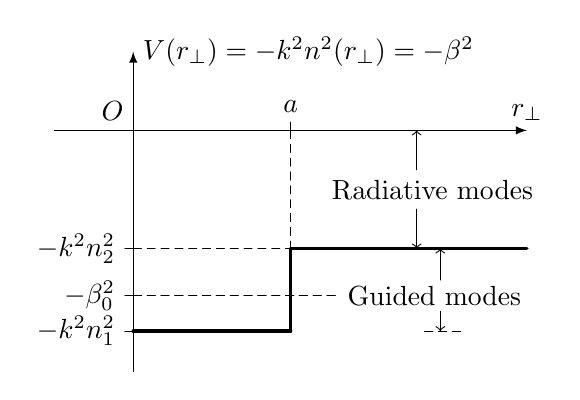
\begin{tikzpicture}[scale=1,cap=round]
% Configurable parameters
\def\k{1.5cm}
\def\eps{1.5*1.7cm}
\def\betasq{1.5*1.4cm}
\def\a{2cm}
\def\maxr{5cm}

% Styles
\tikzstyle{axes}=[arrows={-latex}]
\tikzstyle{auxline}=[densely dashed]
\tikzstyle{important line}=[very thick]

% Coordinates and points.
\coordinate (O) at (0,0);	% Origin.
\coordinate (A) at (\a,0);	% The surface distance to the axis of the fiber.
\coordinate (B) at (0,-\eps);	% -k^2\epsilon at the center of the fiber.
\coordinate (C) at (\a,-\eps);	% -k^2\epsilon on the surface of the fiber.
\coordinate (D) at (0,-\betasq);	% -\beta^2 point at the center of the fiber.
\coordinate (E) at (\a*1.3,-\betasq);	% -\beta^2 point at the end of the maximum r.
\coordinate (F) at (0,-\k);	% -k^2 point at the center of fiber.
\coordinate (G) at (\a,-\k); 	% -k^2 point on the surface of the fiber.
\coordinate (H) at (\maxr,-\k); 	% -k^2 point at the end of r.

% The graphic
 % help grid
% \draw[style=help lines,step=0.5cm] (-2.0,-2.0) grid (2.0,2.0);
  
% Draw axes and marks.
\draw [axes] (-1cm, 0) -- (\maxr,0) node [above] {$r_{\perp}$};
\draw [axes] (0, -1.2*\eps) -- (0, 1.0cm) node [right] {$V(r_{\perp})=-k^2n^2(r_{\perp})=-\beta^2$};
\draw (O) node [above left] {$O$};
\draw[thin] (A) -- (\a,3pt) node[anchor=south] {$a$}; 
\draw (B) -- (-3pt,-\eps) node[anchor=east] {$-k^2n_1^2$};
\draw (D) -- (-3pt,-\betasq) node[anchor=east] {$-\beta_0^2$};
\draw (F) -- (-3pt,-\k) node[anchor=east] {$-k^2n_2^2$};

% Draw potential lines.
\draw[important line] (B) -- (C);
\draw[important line] (C) -- (G);
\draw[important line] (G) -- (H);
\draw[auxline] (D) -- (E) node[right] {Guided modes};
\draw[auxline,very thin] (F) -- (G);
\draw[auxline,very thin] (A) -- (G);

% Other labels and auxlines.
%\draw[<->] (\a*1.25,0) -- (\a*1.25,-\k) node[midway,right] {Scattered modes};
\draw (\a*1.2,-\k/2) node[right] {Radiative modes};
\draw[<-] (\a*1.8,0) -- (\a*1.8,-0.5cm);
\draw[->] (\a*1.8,-1cm) -- (\a*1.8,-\k);
\draw[<-] (\a*1.95,-\k) -- (\a*1.95,-\k-0.4cm);
\draw[->] (\a*1.95,-\k-0.8cm) -- (\a*1.95,-\eps);
\draw[auxline] (\a*1.85,-\eps) -- (\a*2.08,-\eps);
\end{tikzpicture}
}
\caption{Bound and unbound states for the nanofiber eigenvalue 
problem. $ \varepsilon(r\!_\perp)=\varepsilon_{f} =n_1^2$ if $ r_\perp < a $; otherwise, $\varepsilon
(r\!_\perp) =1 $. The parameter $ a $ is the radium of the nanofiber.}
\label{Figs/scatteredmode}
\end{figure}

Using the relationship that
\begin{align}
\nabla^2 \!_\perp = \frac{1}{r_{\!\perp}}\pp{}{r\!_\perp}\! \left(r\!_\perp \pp{}{r\!_\perp} \right) + 
\frac{1}{r_\perp^2} \spp{}{\phi},
\end{align}
and the symmetry of the fiber,  we can  separate the mode function by
\begin{align}
\psi(r\!_\perp,\phi)=\mathcal{E}_{z,\beta m}(r\!_\perp)e^{im\phi},
\end{align} 
and hence
\begin{align}
\mathcal{E}_z(r\!_\perp,\phi,z) = \mathcal{E}_{z,\beta m}(r\!_\perp)e^{i(m\phi+\beta z)},
\end{align}
where $ \mathcal{E}_{z,\beta m}(r\!_\perp) $ satisfies the Bessel's equation
\begin{align}
\left[ \spp{}{r\!_\perp}+ \frac{1}{r_{\!\perp}}\pp{}{r\!_\perp}- 
\frac{m^2}{r^2\!_\perp} + (k^2\varepsilon(r\!_\perp)-\beta^2) \right] 
\mathcal{E}_{z,\beta m}(r\!\!_\perp)=0
\end{align}
with 
\begin{align}
\varepsilon(r\!\!_\perp) = 
\begin{cases}
1, & r\!_\perp>a\\
\varepsilon_f, & r\!_\perp\leq a.
\end{cases}
\end{align}
The general solution for $ \mathcal{E}_{z,\beta m}(r\!\!_\perp) $ can be given in three cases 
corresponding to different 
boundary conditions
\begin{align}
\mathcal{E}_{z,\beta m}(r\!\!_\perp) = \begin{cases}
AJ_m(qr\!\!_\perp) + B Y_m(qr\!_\perp)&\rightarrow J_m(\theta)\sim \cos\theta,\, Y_m(\theta)\sim 
\sin\theta.\\
CI_m(qr\!_\perp) + DK_m(qr\!_\perp) & \rightarrow I_m(\theta) \sim e^\theta,\, K_m(\theta) \sim 
e^{-\theta}.\\
EH_m^{(\!1\!)}(qr\!_\perp) \!+\! FH_m^{(\!2\!)}(qr\!_\perp ) & \rightarrow H_m^{(\!1\!)} (\theta) \! \sim \! 
e^{i\theta},\, 
H_m^{(\!2\!)}(\theta)\!\sim\! e^{\!-i\theta}.
\end{cases}
\end{align}
The positive parameter $ 1/q $ is the characteristic decay length corresponding to $ 1/h_{11} $ and $ 
1/q_{11} $ 
in the $\text{HE}_{11}$ mode expression. Using the symmetric and convergent condition at $ 
r\!_\perp=0\,\text{and}\, \infty $, as for bound modes, for example, if $k< \beta\leq 
k\sqrt{\varepsilon_f}$,
\begin{align}
\left\{
 \begin{array}{lcll}
	r\!_\perp \leq a, & \mathcal{E}_{z,\beta m}(r\!_\perp )\!=\! AJ_m(h r\!_\perp), & h \!=\! 
	\sqrt{k^2\varepsilon_f-\beta^2}\! >\! 0;\\
	r\!_\perp > a, & \mathcal{E}_{z,\beta m}(r\!_\perp )\!=\!DK_m(q r\!_\perp), & q\!=\! 
	\sqrt{\beta^2-k^2}>0.
 \end{array}\right.
\end{align}
Both $ \beta $ and $ h $ are discrete for bound modes. 
For scattered modes, $ 0\leq \beta< k $, similarly, 
\begin{align}
\left\{
 \begin{array}{lcll}
	r\!_\perp \leq a, & \mathcal{E}_{z,\beta m}(r\!_\perp )\!=\! AJ_m(h r\!_\perp), & h \!=\! 
	\sqrt{k^2\varepsilon_f-\beta^2}\! >\! 0;\\
	r\!_\perp > a, & \mathcal{E}_{z,\beta m}(r\!_\perp )\!=\!EH_m^{(\!1\!)}(p r\!_\perp\!), & p\!\!=\!\! 
	\sqrt{k^2-\beta^2}>0.
 \end{array}\right.
\end{align}
Both $ \beta $ and $ p $ are continuous. 
%\textcolor{red}{(Double check the general solutions and the consistence with Equ.~\ref{ET0Rexpand}.)}
%Notice that Ref.\cite{Snyder1983} used $ J_m(hr\!_\perp)\cos m\phi $ and $ 
%(J_m(pr\!_\perp)+CH_m^{(\!1\!)})\cos m\phi $ as the basis for the general solution of $ e $ and $ o $ 
%light 
%of the radiation modes, and summed them up. They are equivalent to the solution here.  

If $ \beta $ is a pure imaginary number, the field will have an exponential decay amplitude on $ z $-direction, and will spread the energy away from the fiber axis. Reference~\cite{Snyder1983} denotes the modes with pure imaginary $ \beta $ as evanescent modes. If $ \beta $ has both real and imaginary parts, the modes are denoted as leaky modes, which are combinations of radiation modes and evanescent modes. Except for the case that the incident light is highly directed at the complementary critical angle $ \theta_c $ of geometric optics, only the radiation modes part can propagate for a long distance along the fiber axis. In our nanofiber system, we only consider the bound and radiation modes. The ranges of some waveguide parameters are given in Table~\ref{tab:fiberparameters}. 
In the table, we have defined the normalized wave number\cite{Snyder1983}, or 
$V$-number\index{$V$-number} 
of a fiber as $V  = 
k_f a \mathrm{NA}$.  Here $k_f=\frac{2\pi}{\lambda}$, is the free space wave number, $a$ is the radius 
of the core of the fiber, and $\mathrm{NA}$ is the numerical aperture\index{numerical aperture} of 
the fiber, $\mathrm{NA} = 
(n_{core}^2 - n_{cladding}^2)^{1/2} = n_{core}(2\Delta)^{1/2}$, with profile height 
parameter\index{profile height parameter} 
$\Delta =\frac{1}{2}(1-n_{cladding}^2/n_{core}^2)\approx (n_{core}-n_{cladding})/n_{core}$.  For 
different modes labeled with $ j $, we always have $V_j^2=a^2(h_j^2+q_j^2)$ and $ \lambda\beta_j/2\pi $ is a mode invariance.  The TE and TM modes have non-vanishing cut-off 
frequencies, as $ a\rightarrow 0 $.  The cutoff frequency is found from $V = a\omega (\Delta)^{1/2}/c =2.405$ for silicon fiber.  
Only the lowest HE mode, $\mathrm{HE}_{11}$, has no cutoff frequency as $ a\rightarrow 0 $.  For $0 < V < 2.405$, which is the case of the nanofiber we are studying, it is the only mode that propagates in the 
fiber. For fixed $ \varepsilon_f $, in the range that $ 0\leq \beta \leq 
k\sqrt{\varepsilon_f} $, we can distinguish the radiative and bound mode as follows:
\begin{align}
\begin{cases}
0\leq \beta < k, &\rightarrow \textit{unbounded radiative modes;}\\
k< \beta \leq k \sqrt{\varepsilon_f}, &\rightarrow \exists a,\, \textit{HE}_{11}\, \textit{is the only 
bound mode.}
\end{cases}
\end{align}


\begin{minipage}{0.97\textwidth}
\centering
\captionof{table}{Ranges of fiber parameters for different modes. } \label{tab:fiberparameters} 
\begin{tabular}{|l|c|c|c|}
\hline  & $\beta$ & $h$ & $p$ \\ 
\hline Bound modes & $k<\beta_j \leq k\sqrt{\varepsilon_f} $ & $ 0\leq h_j<V/a $ & $ p^r_j=0,\, p^i_j>0 $ \\ 
\hline Radiation modes & $0\leq \beta<k$ & $V/a < h\leq k\sqrt{\varepsilon_f}$ & $0<p\leq k $\\ 
\hline Evanescent modes & $ \beta^r=0,\, \beta^i>0 $ & $ k\sqrt{\varepsilon_f} < h $ & $ k<p $ \\ 
\hline 
\end{tabular} 
\par
\bigskip
%The caption:
Superscripts $ r $ and $ i $ denote real and imaginary parts. Subscripts $ j $ denotes the discrete indeces for bound modes. Adapted from Ref.~\cite{Snyder1983} P.P.516 Table 25-1. This can also be understood in geometric optics as shown in Fig.(\ref{fig:Fibermodes}).
\end{minipage}
\bigskip

\begin{figure}
\centering\makebox[\textwidth]{
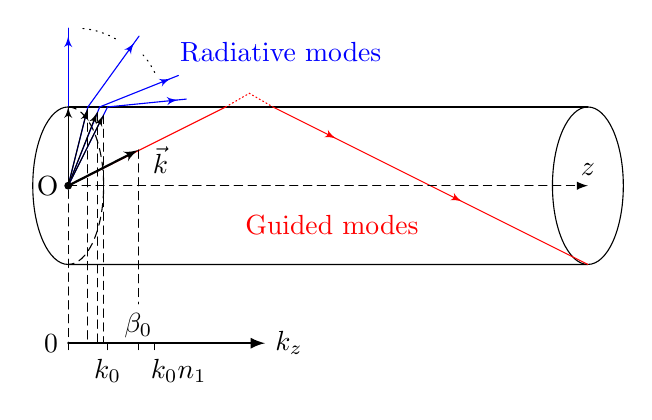
\begin{tikzpicture}[scale=1,cap=round]
% Configurable parameters
\def\fiberrad{1cm}	% Radius of the nanofiber.
\def\comprad{0.45cm}	% Compressed radius of the nanofiber in the view angle.
\def\fiberleftx{0}	% The x-coordiante of the center of the left surface of the fiber.
\def\fiberlefty{0}	% The y-coordiante of the center of the left surface of the fiber.
\def\fiberlength{6.6cm} % The length of the fiber.

% Styles
\tikzstyle{axes}=[arrows={-latex}]
\tikzstyle{auxline}=[densely dashed]
\tikzstyle{important line}=[thick]
\tikzstyle{dot}=[circle,inner sep=1pt,fill,label={#1},name=#1]

% Coordinates and points.
\coordinate (O) at (0,0);	% Origin.
\coordinate (LO) at (\fiberleftx,\fiberlefty); % Center of the left-side surface of the nanofiber.
\coordinate (RO) at (\fiberleftx+\fiberlength,\fiberlefty); % Center of the right-side surface
\coordinate (A) at ({\fiberleftx},{\fiberlefty+\fiberrad});	% Top-left point of the nanofiber.
\coordinate (B) at ({\fiberleftx+\fiberlength},{\fiberlefty+\fiberrad});	% Top-right point of the nanofiber.
\coordinate (C) at ({\fiberleftx+\fiberlength},{\fiberlefty-\fiberrad});	% Bottom-right point of the fiber.
\coordinate (D) at ({\fiberleftx},{\fiberlefty-\fiberrad});	% Bottom-left point of the nanofiber.

% The graph.
% help grid
% \draw[style=help lines,step=0.5cm] (-2.0,-2.0) grid (2.0,2.0);

% Draw the fiber.
\begin{scope} 
    % Outer edge.
    %\fill[left color=purple!50!black,right color=purple!50!black,middle 
%color=purple!50,shading=axis,opacity=0.25] (A) -- (B) arc (90:270:{\comprad} and {\fiberrad}) -- (D) arc 
%(270:90:{\comprad} and {\fiberrad});
    % Right-side surface.
    %\fill[top color=purple!90!,bottom color=purple!2,middle color=purple!30,shading=axis,opacity=0.25] 
%(RO) circle [x radius={\comprad}, y radius = {\fiberrad}];
    % Draw lines of all edges.
    \draw (A) -- (B);
    \draw  (RO) circle [x radius = {\comprad}, y radius =  {\fiberrad}];
    \draw (C) -- (D) arc (270:90:{\comprad} and {\fiberrad}); 
    \draw[densely dashed] (A) arc (90:-90:{\comprad} and {\fiberrad});
\end{scope}

% Draw the guide mode wave vector and propagation lines.
% First part of the ray: up-solid line.
\draw[red] (O)--(2.0*\fiberrad,\fiberrad);
%\draw[red,decoration={ markings,  % This schema allows for fine-tuning the arrows.
%      mark=at position 0.5 with {\arrow{latex'}}, 
%      mark=at position 0.82 with {\arrow{latex'}}},postaction={decorate}] (O) -- (2.0*\fiberrad,\fiberrad)-- (6.0*\fiberrad,-\fiberrad);
% The penetration part of ray: dashed line.
\draw[red,densely dotted] (2.0*\fiberrad,\fiberrad) -- (2.3*\fiberrad,1.1732*\fiberrad) -- (2.6*\fiberrad,\fiberrad);
% The reflected part: solid downarrow.
\draw[red,decoration={ markings,  % This schema allows for fine-tuning the arrows.
      mark=at position 0.2 with {\arrow{latex'}}, 
      mark=at position 0.6 with {\arrow{latex'}}},postaction={decorate}] (2.6*\fiberrad,\fiberrad)-- (6.6*\fiberrad,-\fiberrad);
% The ruler part.
\draw[important line,-latex'] (O) --(27:1) node[below,xshift=8,yshift=5] {$ \vec{k} $};
\draw[auxline] (27:1) -- ({cos(27)},-1.5)  node [below] {$\beta_0$};

% Draw radiation modes.
% Radiation ray 1:
\draw[blue,decoration={ markings,  % This schema allows for fine-tuning the arrows. 
      mark=at position 0.95 with {\arrow{latex'}}},postaction={decorate}] (O) -- (0.5,\fiberrad) -- (1.5,\fiberrad*1.1);
\draw[-latex'] (O)--(63.5:1);
\draw[auxline] (63.5:1) -- ({cos(63.5)},-2);
% Radiation ray 2:
\draw[blue,decoration={ markings,  % This schema allows for fine-tuning the arrows. 
      mark=at position 0.95 with {\arrow{latex'}}},postaction={decorate}] (O) -- (0.4,\fiberrad) -- (1.4,\fiberrad*1.4);
\draw[-latex'] (O)--(68.5:1);
\draw[auxline] (68.5:1) -- ({cos(68.5)},-2);
% Radiation ray 3:
\draw[blue,decoration={ markings,  % This schema allows for fine-tuning the arrows. 
      mark=at position 0.95 with {\arrow{latex'}}},postaction={decorate}] (O) -- (0.25,\fiberrad) -- (0.9,\fiberrad*1.9);
\draw[-latex'] (O)--(76:1);
\draw[auxline] (76:1) -- ({cos(76)},-2);
% Radiation ray 3:
\draw[blue,decoration={ markings,  % This schema allows for fine-tuning the arrows. 
      mark=at position 0.95 with {\arrow{latex'}}},postaction={decorate}] (O)-- (0,2*\fiberrad);
\draw[-latex'] (O) -- (0,\fiberrad);
% Draw dots inbetween.
\draw[dotted] ([shift=(26:1)] 0.2,1.0*\fiberrad) arc (26:45:1);
\draw[dotted] ([shift=(60:1)] 0.1,1.0*\fiberrad) arc (60:89:1);

% Labels and denotes.
\draw (O) node[dot] {};
\draw (O) node[left] {O};
\draw[auxline,-latex] (O) -- (\fiberlength*1.0,0) node [above] {$ z $};	% Z axis line.
\draw[auxline] (0,\fiberrad) -- (0,-2);
\draw[important line,-latex] (0,-2) node[left] {$ 0 $}--(2.5,-2) node[right] {$ k_z $};% kz axis.
\draw (0,-2) -- (0,-2.08);
\draw (0.5,-2) -- (0.5,-2.08) node [anchor=north] {$k_0$};
\draw ({cos(27)},-2) -- ({cos(27)},-2.08);
\draw (1.1,-2) -- (1.1,-2.08) node [below right,xshift=-5] {$k_0n_1$};
\draw (3.35,-0.5) node[red] {Guided modes};	% Guided modes label.
\draw (2.7,1.7*\fiberrad) node[blue] {Radiative modes};	% Radiative modes label.
\end{tikzpicture}
}
\caption{Fiber modes classified through the $ z $-component of the wave vector.}
\label{fig:Fibermodes}
\end{figure}

Due to the symmetry of equations, we also have
\begin{align}
\mathcal{B}_z(r\!_\perp,\phi,z) = \mathcal{B}_{z,\beta m}(r\!_\perp)e^{i(m\phi+\beta z)},
\end{align}
where $  \mathcal{B}_{z,\beta m}(r\!_\perp) $ satisfies the same Bessel's equation as above. 

Next, we consider the case that an atom--which can be treated as an electric dipole in the regime we are interested in--is placed next to the 
nanofiber. Equ.~\eqref{Esrt0} can be rewritten as 
\begin{align}
\boldsymbol{\mathcal{E}}(\br) &= \boldsymbol{\mathcal{E}}_{source}(\br) + 
\boldsymbol{\mathcal{E}}_{ref}(\br)+\boldsymbol{\mathcal{E}}_{tran}(\br)\\
&=
	\begin{cases}
	  \boldsymbol{\mathcal{E}}_{dipole} (\br)+ \boldsymbol{\mathcal{E}}_{ref}(\br) & r\!_\perp \geq a,\\
	  \boldsymbol{\mathcal{E}}_{tran}(\br) & r\!_\perp<a.
	\end{cases} \\
&=
	\begin{cases}
		  \boldsymbol{\mathcal{E}}^{(0)} (\br)+ \boldsymbol{\mathcal{E}}^{(R)}(\br) & r\!_\perp \geq a,\\
		  \boldsymbol{\mathcal{E}}^{(T)}(\br) & r\!_\perp<a.
		\end{cases} \label{Etotalfiber}
\end{align}


For longitudinal components of the electrical and magnetic fields we expand them as follows
\begin{subequations}\label{ET0Rexpand}
\begin{align}
\mathcal{E}^{(T)}_z &= \sum_{m=-\infty}^\infty \int \mathrm{d}\beta e^{im(\phi-\phi') + i\beta (z-z')} \mathcal{E}^{(T)}_{z,m\beta}(r\!_\perp)\\
&= \sum_{m=-\infty}^\infty \int \mathrm{d}\beta e^{im(\phi-\phi') + i\beta (z-z')} c_{m\beta} J_m (hr\!_\perp),\\
% + B_{m\beta} Y_m(hr\!_\perp)\right],\\
\mathcal{E}^{(0)}_{z} &= \sum_{m=-\infty}^\infty \int \mathrm{d}\beta e^{im(\phi-\phi') + i\beta (z-z')} \mathcal{E}^{(0)}_{z,m\beta}(r\!_\perp)\\
\mathcal{E}^{(R)}_z &= \sum_{m=-\infty}^\infty \int \mathrm{d}\beta e^{im(\phi-\phi') + i\beta (z-z')} \mathcal{E}^{(R)}_{z,m\beta}(r\!_\perp)\\
&= \sum_{m=-\infty}^\infty \int \mathrm{d}\beta e^{im(\phi-\phi') + i\beta (z-z')} a_{m\beta} H_m^{(1)} (pr\!_\perp),
\end{align}
\end{subequations}
\begin{subequations}\label{BT0Rexpand}
\begin{align}
\mathcal{B}^{(T)}_z &= \sum_{m=-\infty}^\infty \int \mathrm{d}\beta e^{im(\phi-\phi') + i\beta (z-z')} \mathcal{B}^{(T)}_{z,m\beta}(r\!_\perp)\\
&= \sum_{m=-\infty}^\infty \int \mathrm{d}\beta e^{im(\phi-\phi') + i\beta (z-z')} d_{m\beta} J_m (hr\!_\perp),\\
% + E_{m\beta} Y_m(hr\!_\perp)\right],\\
\mathcal{B}^{(0)}_{z} &= \sum_{m=-\infty}^\infty \int \mathrm{d}\beta e^{im(\phi-\phi') + i\beta (z-z')} \mathcal{B}^{(0)}_{z,m\beta}(r\!_\perp)\\
\mathcal{B}^{(R)}_z &= \sum_{m=-\infty}^\infty \int \mathrm{d}\beta e^{im(\phi-\phi') + i\beta (z-z')} \mathcal{B}^{(R)}_{z,m\beta}(r\!_\perp)\\
&= \sum_{m=-\infty}^\infty \int \mathrm{d}\beta e^{im(\phi-\phi') + i\beta (z-z')} b_{m\beta} H_m^{(1)} (pr\!_\perp),
\end{align}
\end{subequations}
where the subscripts indicate the field components of reflection ($R$), dipole oscillation in free space ($0$) and transmission ($ T $). Notice that we have chosen $ m=\pm 1 $, as the nanofiber can only support HE$_{11}$ modes. 
The $ r\!_\perp $ and $ \phi $ components of the fields can be obtained using Equ.~\eqref{EHzgauss} and $ \mathcal{B}=\mathcal{H} $ in Gauss units for given $ m $. Also notice, in the nanofiber case we are studying, we can define $ z'=0 $ and $ \phi'=0 $, and hence the factor $ e^{im(\phi-\phi') + i\beta (z-z')} $ in the equations above becomes $ e^{im\phi + i\beta z} $. That is what Klimov and others have used in their paper.

The free space dipole emits an electromagnetic field described by
\begin{align}
\mathcal{A} &= -ik \mathbf{d}_0 \frac{e^{ik|\br-\br'|}}{|\br-\br'|},
\end{align}
\begin{align}
\mathcal{B}^{(0)} &= \nabla\times \mathcal{A}\nonumber \\
&=-ik\nabla(\frac{e^{ik|\br-\br'|}}{|\br-\br'|})\times\mathbf{d}_0=-ik\nabla G_0(\br,\br')\times\mathbf{d}_0\nonumber\\
&=\quad\left[\frac{d_z}{r\!_\perp}\pp{G_0(\br,\br')}{\phi}\!-\! d_\phi\pp{G_0(\br,\br')}{z}\right]\mathbf{e}_{r\!_{\perp}}\nonumber\\
&\quad+\left[d_{r\!_\perp}\pp{G_0(\br,\br')}{z}\!-\!d_z\pp{G_0(\br,\br')}{r\!_\perp} \right]\mathbf{e}_\phi \nonumber\\
&\quad+ \left[d_\phi\pp{G_0(\br,\br')}{r\!_\perp}\!-\! \frac{d_{r\!_\perp}}{r\!_\perp}\pp{G_0(\br,\br')}{\phi} \right]\mathbf{e}_z\\
&=\mathcal{B}^{(0)}_{r\!_\perp}\mathbf{e}_{r\!_{\perp}} +\mathcal{B}^{(0)}_\phi\mathbf{e}_\phi + \mathcal{B}^{(0)}_z\mathbf{e}_z,\\
\mathcal{E}^{(0)} &= \frac{i}{k} \nabla\times \mathcal{H}^{(0)}=\frac{i}{k}\nabla\times \mathcal{B}^{(0)}\nonumber\\
&=\frac{i}{k}(\frac{1}{r\!_\perp}\!\pp{\mathcal{B}^{(\!0\!)}_z}{\phi}\!-\! \pp{\mathcal{B}^{(\!0\!)}_\phi}{z})\mathbf{e}_{r\!_{\perp}} \!\!+\! \frac{i}{k}(\!\pp{\mathcal{B}^{(\!0\!)}_{r\!_\perp}}{z} \!-\! \pp{\mathcal{B}^{(\!0\!)}_z}{r\!_\perp})\mathbf{e}_\phi \!\!+\! \frac{i}{r\!_\perp\! k} (\!\pp{(\! r\!_\perp \mathcal{B}^{(\!0\!)}_\phi)}{r\!_\perp} \!\!-\!\! \pp{\mathcal{B}^{(\!0\!)}_{r\!_\perp}}{\phi}\! )\mathbf{e}_z\\
&=\mathcal{E}^{(0)}_{r\!_\perp}\mathbf{e}_{r\!_{\perp}} +\mathcal{E}^{(0)}_\phi\mathbf{e}_\phi + \mathcal{E}^{(0)}_z\mathbf{e}_z,
\end{align}
or, by Equ.~\eqref{EGd}. Here, $ \mathbf{d}_0 $ is the dipole momentum in vacuum. We denote $d_{r\!_\perp},\, d_\phi$ and $d_z$ as the cylindrical components of the dipole momentum at arbitrary observation point ${\rm {\bf r}}=\left( {r\!_\perp ,\phi ,z}\right) $; while we use $d^0_{r\!_\perp}$, $d^0_\phi$ and $d^0_z$ to indicate the cylindrical components of the dipole momentum at the dipole position ${\rm 
{\bf {r}^{\prime }}}=\left( {{r\!_\perp }^{\prime },{\phi }^{\prime },{z}^{\prime }}\right) $. As shown in Fig.(\ref{fig:dipolemomentumtransmission}) on page~\pageref{fig:dipolemomentumtransmission}, we defined the vector from the center of the nanofiber's core pointing to the atom position as $x$-axis, and the rotating symmetric axis of the nanofiber as the $z$-axis. The relationships between the dipole momentum components at $\mathbf{r}$ and $\mathbf{r}'$ can be given by
\begin{align}
d_{r\!_\perp}\! &= \cos(\phi\!-\!\phi')d^0_{r\!_\perp}\!\!+\!\sin(\phi\!-\!\phi')d^0_\phi=\frac{1}{\sqrt{2}}\left(-e^{-i(\phi\!-\!\phi')}d_++e^{i(\phi\!-\!\phi')}d_- \right),\\
d_\phi &=\cos(\phi\!-\!\phi')d^0_\phi\!-\!\sin(\phi\!-\!\phi')d^0_{r\!_\perp}=\frac{i}{\sqrt{2}}\left(e^{-i(\phi\!-\!\phi')}d_++e^{i(\phi\!-\!\phi')}d_- \right),\\
d_z &= d^0_z,
\end{align}
where I have defined the position-independent reduced dipole vector components
\begin{align}
d_\pm \equiv \mp \frac{1}{\sqrt{2}}(d^0_{r\!_\perp}\pm id^0_{\phi}).
\end{align}
The terms associated with $d_\pm$ in the dipole moment formula lower or raise the mode index by $1$. Notice that we have used $\phi\!-\!\phi'$ as the projected angle between $\mathbf{r}$ and $\mathbf{r}'$ to make the relationship work in general. 

\begin{figure}
\centering\makebox[\textwidth]{
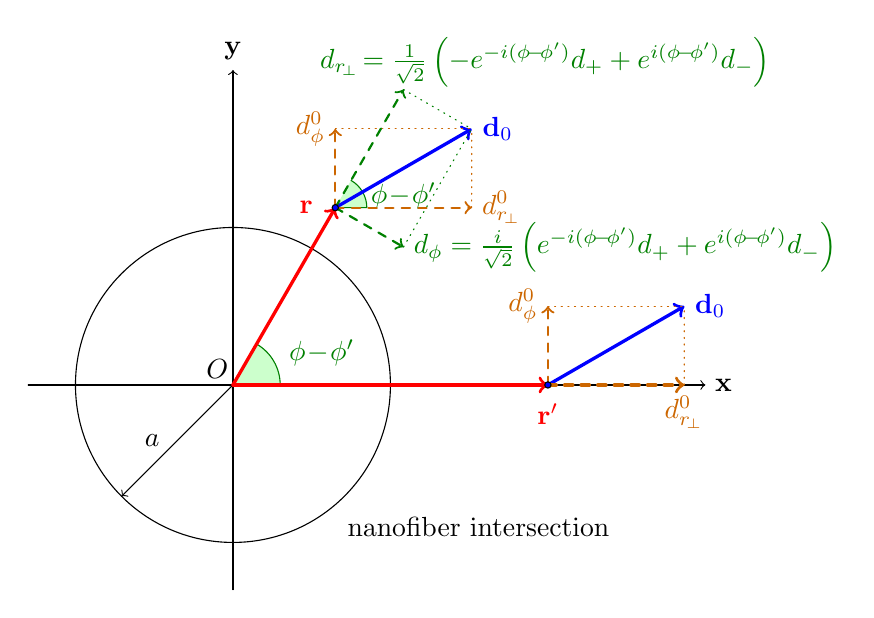
\begin{tikzpicture}[scale=2,cap=round]
% Local definitions
  \def\AngleAtr{60}	% angle of r w.r.t x-axis
  \def\AngleOfd{30}	% angle of d w.r.t. x-axis
  \def\LenOfd{1cm} % length of the dipole momentum vector
  \def\drp{0.8660cm}	% drp at r'
  \def\dphi{0.5cm}	% dphi at r'
  \def\drpr{0.8660}	% drp at r
  \def\dphir{-0.5}	% dphi at r
  \def\Angledrp{\AngleAtr}	% angle of drp w.r.t. x-axis
  \def\Angledphi{150}
  
  \coordinate (O) at (0,0);		% origin
  \coordinate (R) at (2.0cm,0); % position of the dipole at r'
  \coordinate (r) at (\AngleAtr:1.3cm);	% position of observation point

  % Colors
  \colorlet{anglecolor}{green!50!black}
  \colorlet{rvectorcolor}{red}
  \colorlet{assisvectorcolor}{orange!80!black}
  \colorlet{momentumcolor}{blue}

  % Styles
  \tikzstyle{axes}=[]
  \tikzstyle{important line}=[very thick]
  \tikzstyle{information text}=[rounded corners,fill=red!10,inner sep=1ex]

  % The graphic
  % help grid
  %\draw[style=help lines,step=0.5cm] (-2.0,-2.0) grid (2.0,2.0);
  
  % circle for the nanofiber scope
  \draw (0,0) circle (1cm); 
  \draw[<->] (0,0) --node[left=1mm] {$a$} (225:1cm) ;
  \draw (-30:1.8cm) node {\text{nanofiber intersection}};
  % coordinates
  \begin{scope}[style=axes]
    \draw[->] (-1.3cm,0) -- (3.0cm,0) node[right] {$\mathbf{x}$};
    \draw[->] (0,-1.3cm) -- (0,2.0cm) node[above] {$\mathbf{y}$};
    \draw (-1mm,1mm) node {$O$};
  \end{scope}
  
  % angle and position vector for r
  \filldraw[fill=green!20,draw=anglecolor] (0,0) -- (3mm,0pt) arc(0:\AngleAtr:3mm);
    \draw (20:6mm) node[anglecolor] {$\phi\!-\! \phi'$};
  \draw[->,style=important line,rvectorcolor] (O) -- (r) node[left=1.5mm] {$\mathbf{r}$};
  % arc between two decomposition approaches
  \filldraw[fill=green!20,draw=anglecolor] (r.center)--($(r.center)+(2mm,0)$) arc (0:\AngleAtr:2mm);
  \draw ($(r.center)+(10:4.4mm)$) node[anglecolor] {$\phi\!-\! \phi'$};
  % dipole momentum vector at r
  \draw[->,style=important line,momentumcolor] (r) -- +(\AngleOfd:\LenOfd) node[right] {$\mathbf{d}_0$};
  
  % d vector components at r
  \draw[->,dashed,thick,assisvectorcolor] (r) -- +(0:\drp) node[right] {$d^0_{r\!_\perp}$};
  \draw[style=dotted,assisvectorcolor] ($(r.center)+(0:\drp)$) -- ($(r.center)+(\AngleOfd:\LenOfd)$);
  \draw[->,dashed,thick,assisvectorcolor] (r) -- +(90:\dphi) node[left] {$d^0_\phi$};
  \draw[style=dotted,assisvectorcolor] ($(r.center)+(90:\dphi)$) -- ($(r.center)+(\AngleOfd:\LenOfd)$);
  \draw[->,thick,dashed,anglecolor] (r) -- +(\Angledrp:\drpr) node[yshift=8mm,xshift=1.8cm,anchor=north] {$d_{r\!_\perp}\!=\frac{1}{\sqrt{2}}\left(-e^{-i(\phi\!-\!\phi')}d_++e^{i(\phi\!-\!\phi')}d_- \right)$};
  \draw[style=dotted,anglecolor] ($(r.center)+(\Angledrp:\drpr)$) -- ($(r.center)+(\AngleOfd:\LenOfd)$);
  \draw[->,thick,dashed,anglecolor] (r) -- +(\Angledphi:\dphir) node[right] {$d_\phi=\frac{i}{\sqrt{2}}\left(e^{-i(\phi\!-\!\phi')}d_++e^{i(\phi\!-\!\phi')}d_- \right)$};
  \draw[style=dotted,anglecolor] ($(r.center)+(\Angledphi:\dphir)$) -- ($(r.center)+(\AngleOfd:\LenOfd)$);
  \draw [fill=blue] (r) circle (0.2mm) node {}; % starting point at r
   
  % dipole momentum vector for r'
  \draw[->,style=important line,rvectorcolor] (O) -- (R) node[below=1mm] {$\mathbf{r}'$};
  \draw[->,style=important line,momentumcolor] (R) -- +(\AngleOfd:\LenOfd) node[right] {$\mathbf{d}_0$};
  \draw[->,very thick,dashed,assisvectorcolor] (R) -- +(0:\drp) node[below] {$d^0_{r\!_\perp}$};
  \draw[style=dotted,assisvectorcolor] ($(R.center)+(0:\drp)$) -- ($(R.center)+(\AngleOfd:\LenOfd)$);
  \draw[->,thick,dashed,assisvectorcolor] (R) -- +(90:\dphi) node[left] {$d^0_\phi$};
  \draw[style=dotted,assisvectorcolor] ($(R.center)+(90:\dphi)$) -- ($(R.center)+(\AngleOfd:\LenOfd)$);
  \draw [fill=blue] (R) circle (0.2mm) node {}; % starting point at r'
\end{tikzpicture}}
\caption{Dipole momentum decompositions in the $xy$-plane.}
\label{fig:dipolemomentumtransmission}
\end{figure}

Using the expansion of the free-space scalar Green function (Equ.~\eqref{scalarG}) for the space $ \left(r\!_\perp <r_\perp ^{\prime}\right) $ that 
\begin{align}
G_0(\br,\br') &={\frac{{e^{ik{\left| {{\rm {\bf r}}-{\rm {\bf {r}^{\prime }}}}\right| }}}}{{{%
\left| {{\rm {\bf r}}-{\rm {\bf {r}^{\prime }}}}\right| }}}}\nonumber\\
&={\frac{{i}}{{2}}%
}{\sum\limits_{m=-\infty }^{\infty } {{\oint\limits_{C_{1}}{\mathrm{d}\beta \;e^{im\left( {\phi -{\phi }%
^{\prime }}\right) +i\beta \left( {z-{z}^{\prime }}\right) }J_{m}\left( {pr\!_\perp
}\right) H_{m}^{\left( {1}\right) }\left( pr_\perp ^{\prime
}\right) }}}},
\end{align}
and for $ \left(r\!_\perp >r_\perp ^{\prime}\right) $
\begin{align}
G_0(\br,\br') &={\frac{{e^{ik{\left| {{\rm {\bf r}}-{\rm {\bf {r}^{\prime }}}}\right| }}}}{{{%
\left| {{\rm {\bf r}}-{\rm {\bf {r}^{\prime }}}}\right| }}}}\nonumber\\
&={\frac{{i}}{{2}}%
}{\sum\limits_{m=-\infty }^{\infty } {{\oint\limits_{C_{1}}{\mathrm{d}\beta \;e^{im\left( {\phi -{\phi }%
^{\prime }}\right) +i\beta \left( {z-{z}^{\prime }}\right) }J_{m}\left( {pr\!_\perp^{\prime} }\right) H_{m}^{\left( {1}\right) }\left( pr_\perp \right) }}}},
\end{align}
one can obtain the free space dipole radiation field components in Equ.~\eqref{ET0Rexpand} and~\eqref{BT0Rexpand}. The contour $ C_1 $ and field components can be found in Ref.~\cite{Klimov2004}. ~\footnote{Similarly, the decomposition of a plane wave function can be found in Appendix~\ref{Ch:PlanewaveDecomposition}}.

The free radiation field components associated with the $ e^{im\phi+i\beta z} $ term (the $m$-th mode components) for the $r\!_\perp<r'\!_\perp$ region can be given by
\begin{align}
\mathcal{B}_{z,m\beta}^{(0)} &= \frac{ikp}{2\sqrt{2}}J_m(pr\!_\perp)\left[ d_{+} H_{m+1}^{(1)}(pr'\!\!_\perp) \!-\! d_- H_{m-1}^{(1)}(pr'\!_\perp) \right],\\
\mathcal{B}_{\phi,m\beta}^{(0)} &= \frac{ik}{2}\left[ \frac{\beta d_{-}}{\sqrt{2}} J_{m-1}\left( pr\!_\perp \right)H_{m-1}^{(1)}\left( {pr\!_\perp^{\prime} }\right) -\frac{\beta d_+}{\sqrt{2}} J_{m+1}\left( pr\!_\perp \right)H_{m+1}^{(1)}\left( {pr\!_\perp^{\prime} }\right)\right. \nonumber\\ 
&\qquad\quad \left. + \frac{ipd^0_z}{2}\left(J_{m-1}(pr\!_\perp)-J_{m+1}(pr\!_\perp) \right)H_m^{(1)}(pr\!_\perp^{\prime}) \right],\\
\mathcal{B}_{r\!_\perp, m\beta}^{(0)} &= \frac{k}{2}\left[\frac{i m d^0_z}{r\!_\perp} J_m\left( pr\!_\perp \right) H_m^{(1)}\left( {pr\!_\perp^{\prime} }\right) \right. \nonumber\\
&\qquad \left. +\frac{\beta d_+}{\sqrt{2}} J_{m\!+\!1}(pr\!_\perp) H_{m\!+\! 1}^{(1)}(pr\!_\perp^{\prime}) \!+\! \frac{\beta d_-}{\sqrt{2}} J_{m\!-\! 1}(pr\!_\perp)H_{m\!-\!1}^{(1)}(pr\!_\perp^{\prime})   \right],\\
\mathcal{E}_{z,m\beta}^{(0)} 
&= \frac{p}{2}J_{m}\left( pr\!_\perp \right)\left[  id^0_z p H_m^{(1)}\left( {pr\!_\perp^{\prime} }\right) \phantom{\frac{d^0_z}{\sqrt{2}}} \right. \nonumber\\
&\qquad\qquad\qquad \left. + \frac{\beta d_{+}}{\sqrt{2}} H_{m+1}^{(1)}\left( {pr\!_\perp^{\prime} }\right) +\frac{\beta d_-}{\sqrt{2}} H_{m-1}^{(1)}\left( {pr\!_\perp^{\prime} }\right) \right], \\
\mathcal{E}_{\phi,m\beta}^{(0)} 
&= -\frac{im\beta d^0_z}{2r\!_\perp} J_{m}\left( pr\!_\perp \right) H_m^{(1)}\left( {pr\!_\perp^{\prime} }\right) \nonumber\\
&\quad+\frac{d_+}{2\sqrt{2}} \left[ \frac{mp}{r\!_\perp}J_{m}\left( pr\!_\perp \right)-k^2 J_{m+1}\left( pr\!_\perp \right)\right] H_{m+1}^{(1)}\left( {pr\!_\perp^{\prime} }\right) \nonumber\\
&\quad+ \frac{d_-}{2\sqrt{2}}\left[\frac{mp}{r\!_\perp}J_m\!\left( pr_\perp \right)-k^2J_{m-1}\!\left( pr_\perp \right) \right] H_{m-1}^{(1)}\!\left( {pr\!_\perp^{\prime} }\right),\\
\mathcal{E}_{r\!_\perp,m\beta}^{(0)} 
&= \frac{\beta pd^0_z}{4}\left[ J_{m+1}\!\left( pr\!_\perp \right)-J_{m-1}\!\left( pr_\perp \right)\right] H_m^{(1)}\left( {pr\!_\perp^{\prime} }\right)\nonumber\\ 
&\quad -\frac{d_+}{2\sqrt{2}}\left[ i\beta^2J_{m+1}\!\left( pr_\perp \right) +\frac{imp}{r\!_\perp}J_m\!\left( pr_\perp \right)\right] H_{m+1}^{(1)}\!\left( {pr\!_\perp^{\prime} }\right)\nonumber\\
&\quad + \frac{d_-}{2\sqrt{2}}\left[ i\beta^2J_{m-1}\!\left( pr_\perp \right) +\frac{imp}{r\!_\perp}J_m\!\left( pr_\perp \right)\right] H_{m-1}^{(1)}\!\left( {pr\!_\perp^{\prime} }\right).
\end{align}
More details on deriving the E-field components can be found in \textit{Derivation of free-space E-field components.pdf}. Some properties of Bessel functions are used in deriving these expressions (see appendix). 

By exchanging $J_m$ and $H_m^{(1)}$ functions, one can also obtain the field components that the reference~\cite{Klimov2004} did not include for the case of $ r\!_\perp>r'\!_\perp $. The magnetic and electrical fields components for $ \br\!_\perp>\br'\!_\perp $ are 
\begin{align}
\mathcal{B}_{z,m\beta}^{(0)} &= \frac{ikp}{2\sqrt{2}}H^{(1)}_m(pr\!_\perp)\left[ d_{+} J_{m+1}(pr'\!\!_\perp) \!-\! d_- J_{m-1}(pr'\!_\perp) \right],\\
\mathcal{B}_{\phi,m\beta}^{(0)} &= \frac{ik}{2}\left[ \frac{\beta d_{-}}{\sqrt{2}} H^{(1)}_{m-1}\left( pr\!_\perp \right)J_{m-1}\left( {pr\!_\perp^{\prime} }\right) -\frac{\beta d_+}{\sqrt{2}} H^{(1)}_{m+1}\left( pr\!_\perp \right)J_{m+1}\left( {pr\!_\perp^{\prime} }\right)\right. \nonumber\\ 
&\qquad\quad \left. + \frac{ipd^0_z}{2}\left(H^{(1)}_{m-1}(pr\!_\perp)-H^{(1)}_{m+1}(pr\!_\perp) \right)J_m(pr\!_\perp^{\prime}) \right],\\
\mathcal{B}_{r\!_\perp, m\beta}^{(0)} &= \frac{k}{2}\left[\frac{i m d^0_z}{r\!_\perp} H^{(1)}_m\left( pr\!_\perp \right) J_m\left( {pr\!_\perp^{\prime} }\right) \right. \nonumber\\
&\qquad \left. +\frac{\beta d_+}{\sqrt{2}} H^{(1)}_{m\!+\!1}(pr\!_\perp) J_{m\!+\! 1}(pr\!_\perp^{\prime}) \!+\! \frac{\beta d_-}{\sqrt{2}} H^{(1)}_{m\!-\! 1}(pr\!_\perp) J_{m\!-\!1}(pr\!_\perp^{\prime})   \right],\\
\mathcal{E}_{z,m\beta}^{(0)} 
&= \frac{p}{2}H^{(1)}_{m}\left( pr\!_\perp \right)\left[  id^0_z p J_m\left( {pr\!_\perp^{\prime} }\right) \phantom{\frac{d^0_z}{\sqrt{2}}} \right. \nonumber\\
&\qquad\qquad\qquad \left. + \frac{\beta d_{+}}{\sqrt{2}} J_{m+1}\left( {pr\!_\perp^{\prime} }\right) +\frac{\beta d_-}{\sqrt{2}} J_{m-1}\left( {pr\!_\perp^{\prime} }\right) \right], \\
\mathcal{E}_{\phi,m\beta}^{(0)} 
&= -\frac{im\beta d^0_z}{2r\!_\perp} H^{(1)}_{m}\left( pr\!_\perp \right) J_m\left( {pr\!_\perp^{\prime} }\right) \nonumber\\
&\quad+\frac{d_+}{2\sqrt{2}} \left[ \frac{mp}{r\!_\perp}H^{(1)}_{m}\left( pr\!_\perp \right)-k^2 H^{(1)}_{m+1}\left( pr\!_\perp \right)\right] J_{m+1}\left( {pr\!_\perp^{\prime} }\right) \nonumber\\
&\quad+ \frac{d_-}{2\sqrt{2}}\left[\frac{mp}{r\!_\perp}H^{(1)}_m\!\left( pr_\perp \right)-k^2 H^{(1)}_{m-1}\!\left( pr_\perp \right) \right] J_{m-1}\!\left( {pr\!_\perp^{\prime} }\right),\\
\mathcal{E}_{r\!_\perp,m\beta}^{(0)} 
&= \frac{\beta pd^0_z}{4}\left[ H^{(1)}_{m+1}\!\left( pr\!_\perp \right)-H^{(1)}_{m-1}\!\left( pr_\perp \right)\right] J_m\left( {pr\!_\perp^{\prime} }\right)\nonumber\\ 
&\quad -\frac{d_+}{2\sqrt{2}}\left[ i\beta^2H^{(1)}_{m+1}\!\left( pr_\perp \right) +\frac{imp}{r\!_\perp}H^{(1)}_m\!\left( pr_\perp \right)\right] J_{m+1}\!\left( {pr\!_\perp^{\prime} }\right)\nonumber\\
&\quad + \frac{d_-}{2\sqrt{2}}\left[ i\beta^2H^{(1)}_{m-1}\!\left( pr_\perp \right) +\frac{imp}{r\!_\perp}H^{(1)}_m\!\left( pr_\perp \right)\right] J_{m-1}\!\left( {pr\!_\perp^{\prime} }\right).
\end{align}


The expressions above are formally different from Klimov's paper, but are consistent with Nha's paper~\cite{Nha1997}. By using some identities of Bessel functions, one should be able to reproduce Klimov's expressions, which we have checked numerically equivalent to our results.

By using the boundary conditions at $ r\!_\perp=a $ and Equ.~\ref{Etotalfiber} that
\begin{align}
%\varepsilon_f \mathcal{E}_{r\!_\perp}(r\!_\perp =a^> ) = \mathcal{E}_{r\!_\perp}(r\!_\perp =a^< ),\\
\mathcal{E}_{z}(r\!_\perp =a^> ) = \mathcal{E}_{z}(r\!_\perp =a^< ),\\
%\mathcal{B}_{r\!_\perp}(r\!_\perp =a^> ) = \mathcal{B}_{r\!_\perp}(r\!_\perp =a^< ),\\
\mathcal{B}_{z}(r\!_\perp =a^> ) = \mathcal{B}_{z}(r\!_\perp =a^< ),\\
\mathcal{E}_{\phi}(r\!_\perp =a^> ) = \mathcal{E}_{\phi}(r\!_\perp =a^< ),\\
\mathcal{B}_{\phi}(r\!_\perp =a^> ) = \mathcal{B}_{\phi}(r\!_\perp =a^< ),
\end{align}
where $ a^< $ and $ a^> $ denote the boundaries at the sides less and larger than $ a $, and the connections between field components (Equ.(\ref{EHzgauss})), we can obtain all unknown coefficients. In details, the boundary conditions yield
\begin{align}
a_{m\beta}H_m^{(1)}(pa)+\mathcal{E}_{z,m\beta}^{(0)}(r\!_\perp =a ) &= c_{m\beta}J_m(ha),\\
b_{m\beta}H_m^{(1)}(pa)+\mathcal{B}_{z,m\beta}^{(0)}(r\!_\perp =a ) &= d_{m\beta}J_m(ha),\\
\frac{m\! \beta}{p^2\! a}a_{m\!\beta} H\!_m^{(1)}\!(pa)\! &+\! \frac{i\!k}{p^2}\! b\!_{m\!\beta}\! \left. \pp{H\!_m^{( 1 )}(p r\!_\perp)}{r\!_\perp}\! \right|_{r\!_\perp\! =\! a}\!\! -\! \mathcal{E}\! _{\phi,m\! \beta}^{(0)}(r\!_\perp\! =\! a ) \nonumber \\
&= \frac{m\! \beta}{h^2\! a}\! c_{m\! \beta} J\!_m(ha)\! +\! \frac{i\!k}{h^2}\!d\!_{m\!\beta} \! \left. \pp{J\!_m(h r\!_\perp \!)}{r\!_\perp}\! \right|_{r\!_\perp\! =\! a},\\
\frac{m\! \beta}{p^2\! a}b_{m\!\beta} H\!_m^{(1)}\!(pa)\! &+\! \frac{i\!k}{p^2}\! a\!_{m\!\beta}\! \left. \pp{H\!_m^{( 1 )}(p r\!_\perp)}{r\!_\perp}\! \right|_{r\!_\perp\! =\! a}\!\! +\! \mathcal{B}\! _{\phi,m\! \beta}^{(0)}(r\!_\perp\! =\! a ) \nonumber \\
&= \frac{m\! \beta}{h^2\! a}\! d_{m\! \beta} J\!_m(ha)\! +\! \frac{i\!k\varepsilon}{h^2}\!c\!_{m\!\beta} \! \left. \pp{J\!_m(h r\!_\perp \!)}{r\!_\perp}\! \right|_{r\!_\perp\! =\! a}.
\end{align}
One can substitute the first two equations into the last two equations, and obtain a equation set of $a_{m\beta}$ and $b_{m\beta}$ as below:
\begin{align}
&\quad \left[\frac{m\! \beta}{p^2\! a} H\!_m^{(1)}\!(pa) \!-\! \frac{m\! \beta}{h^2\! a}\!H_m^{(1)}(pa) \right] a_{m\!\beta}\nonumber\\
&\quad +\left[\! \frac{i\!k}{p^2}\! \left. \pp{H\!_m^{( 1 )}(p r\!_\perp)}{r\!_\perp}\! \right|_{r\!_\perp\! =\! a}\!\!-\! \frac{i\!k}{h^2J_m(ha)}\! \left. \pp{J\!_m(h r\!_\perp \!)}{r\!_\perp}\! \right|_{r\!_\perp\! =\! a} H_m^{(1)}(pa) \right]b\!_{m\!\beta} \nonumber\\
&= \frac{m\! \beta}{h^2\! a}\! \mathcal{E}_{z,m\beta}^{(0)}(r\!_\perp =a ) \!+\! \! \frac{i\!k}{h^2J_m(ha)}\! \left. \pp{J\!_m(h r\!_\perp \!)}{r\!_\perp}\! \right|_{r\!_\perp\! =\! a}\mathcal{B}_{z,m\beta}^{(0)}(r\!_\perp =a )  \!+\!\mathcal{E}\! _{\phi,m\! \beta}^{(0)}(r\!_\perp\! =\! a )\\
&\quad \left[\frac{m\! \beta}{p^2\! a} H\!_m^{(1)}\!(pa) \!-\! \frac{m\! \beta}{h^2\! a}\!H_m^{(1)}(pa) \right] b_{m\!\beta}\nonumber\\
&\quad +\left[\! \frac{i\!k}{p^2}\! \left. \pp{H\!_m^{( 1 )}(p r\!_\perp)}{r\!_\perp}\! \right|_{r\!_\perp\! =\! a}\!\!-\! \frac{i\!k\varepsilon}{h^2J_m(ha)}\! \left. \pp{J\!_m(h r\!_\perp \!)}{r\!_\perp}\! \right|_{r\!_\perp\! =\! a} H_m^{(1)}(pa) \right]a\!_{m\!\beta} \nonumber\\
&= \frac{m\! \beta}{h^2\! a}\! \mathcal{B}_{z,m\beta}^{(0)}(r\!_\perp =a ) \!+\! \! \frac{i\!k\varepsilon}{h^2J_m(ha)}\! \left. \pp{J\!_m(h r\!_\perp \!)}{r\!_\perp}\! \right|_{r\!_\perp\! =\! a}\mathcal{E}_{z,m\beta}^{(0)}(r\!_\perp =a )  \!-\!\mathcal{B}\! _{\phi,m\! \beta}^{(0)}(r\!_\perp\! =\! a ).
\end{align}

The solutions of $a_{m\beta}$ and $b_{m\beta}$ are given by Equs.(47-50) in Ref.~\cite{Klimov2004}. To summarize, we also have
\begin{align}
a_{m\beta} &= \frac{na}{P^2+QR},\\
b_{m\beta} &= \frac{nb}{P^2+QR},\\
c_{m\beta} &= \frac{\mathcal{E}_{z,m\beta}^{(0)}(r\!_\perp\!=\!a)+ H_m^{(1)}(pa)a_{m\beta}}{J_m(ha)},\\
d_{m\beta} &= \frac{\mathcal{H}_{z,m\beta}^{(0)}(r\!_\perp\!=\!a)+ H_m^{(1)}(pa)b_{m\beta}}{J_m(ha)},
\end{align}
where
\begin{align}
na &= h^2p^2aJ_m(ha)PE_{\phi,m\beta}^{(0)}(r\!_\perp\!=\!a) \nonumber\\
&\quad + p^2\left[J_m(ha)\beta mP+kan_1^2h \dd{}{(ha)}J_m(ha)Q \right] E_{z,m\beta}^{(0)} \nonumber\\
&\quad + ih^2p^2 aJ_m(ha)QB_{\phi,m\beta}^{(0)}(r\!_\perp\!\!=\!a) \!-\! im\beta hpJ_m(ha)SB_{z,m\beta}^{(0)}(r\!_\perp\!\!=\!a),\\
nb &= h^2p^2aJ_m(ha)PB_{\phi,m\beta}^{(0)}(r\!_\perp\!=\!a) \nonumber\\
&\quad + p^2\left[J_m(ha)\beta mP-kah \dd{}{(ha)}J_m(ha)R \right] B_{z,m\beta}^{(0)} \nonumber\\
&\quad + ih^2p^2 aJ_m(ha)RE_{\phi,m\beta}^{(0)}(r\!_\perp\!\!=\!a) \!+\! im\beta hpJ_m(ha)TE_{z,m\beta}^{(0)}(r\!_\perp\!\!=\!a),
\end{align} 
and
\begin{align}
P &=m\beta k^2J_m(ha)H_m^{(1)}(pa)(n_1^2-1),\\
Q &=-hpak\left[ hJ_m(ha)\dd{}{(pa)}H_m^{(1)}(pa)-pH_m^{(1)}(pa)\dd{}{(ha)}J_m(ha) \right],\\
R &=hpak\left[ hJ_m(ha)\dd{}{(pa)}H_m^{(1)}(pa)-pn_1^2H_m^{(1)}(pa)\dd{}{(ha)}J_m(ha) \right],\\
S &=hpak\left[ pJ_m(ha)\dd{}{(pa)}H_m^{(1)}(pa)-hH_m^{(1)}(pa)\dd{}{(ha)}J_m(ha) \right],\\
T &=hpak\left[ pJ_m(ha)\dd{}{(pa)}H_m^{(1)}(pa)-hn_1^2H_m^{(1)}(pa)\dd{}{(ha)}J_m(ha) \right].
\end{align}

\begin{figure}
\begin{minipage}{.91\linewidth}
\centering
\subfloat[]{\label{contourplot_upper}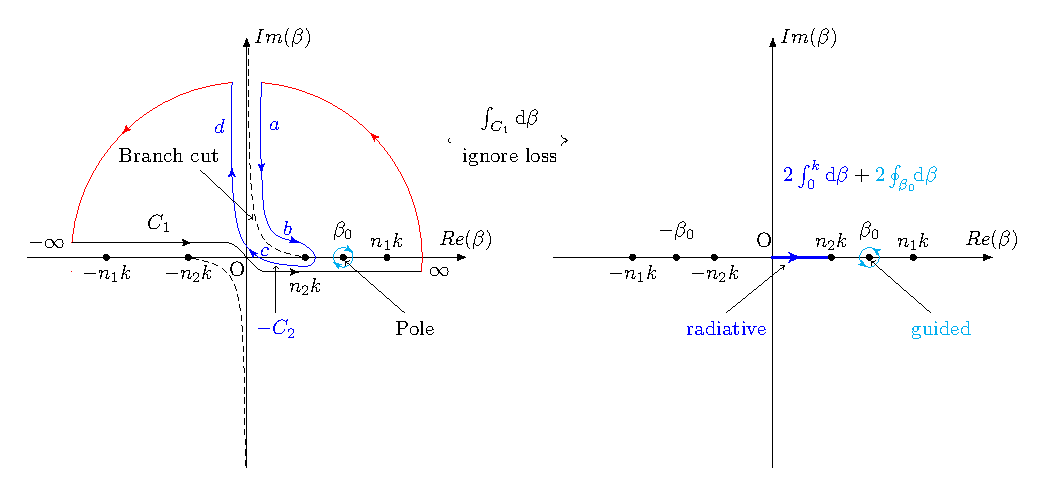
\includegraphics[scale=0.75]{./Figs/contourplot_upper}}
\end{minipage}
\par\medskip
\begin{minipage}{.91\linewidth}
\centering
\subfloat[]{\label{contourplot_lower}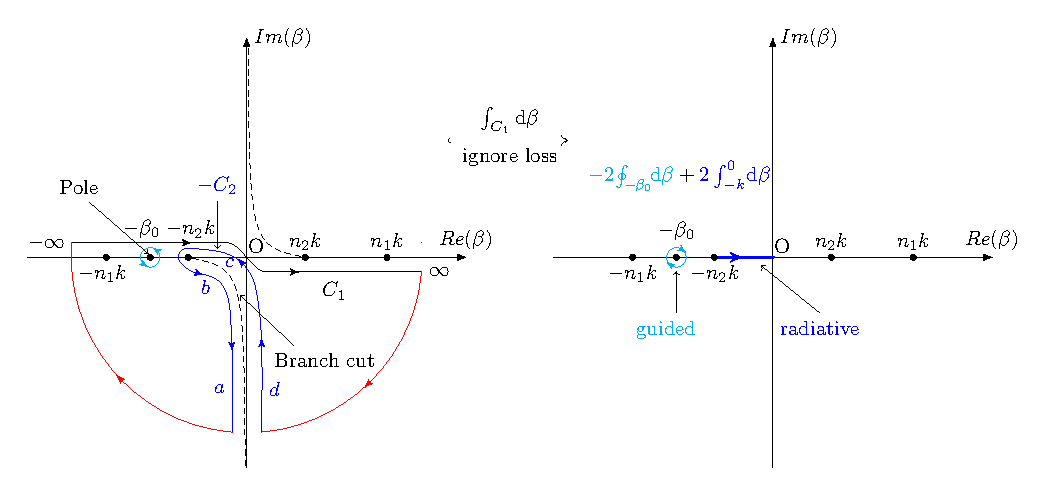
\includegraphics[scale=0.75]{./Figs/contourplot_lower}}
\end{minipage}
\caption{Integration paths. For the case that $ z>0 $, we can use the zero-valued contour integral path drawn in subfig.~\ref{contourplot_upper} to calculate the integration along path $ C_1 $. The simplified integration path by ignoring waveguide losses is given on the right-hand-side. It only contains the forward propagating mode contributions with radiation and guided mode components as divided through the real-axis integral and the loop-hole integral. For the $ z<0 $ case, the contour integral analysis is given in subfig.~\ref{contourplot_lower}, which only includes the backward propagating mode contributions.}
\label{fig:integralpath}
\end{figure}

Now, we only consider the $ m=\pm 1 $ modes, and hence Equs.~\ref{ET0Rexpand}, ~\ref{BT0Rexpand} and the corresponding $ \phi $ and $ r\!_\perp $ components can be explicitly expressed as contour integrals as below
\begin{subequations}\label{ET0RC1}
\begin{align}
\mathcal{E}^{(T)}_z &= \sum_{m=\pm 1} \int_{C_1} \mathrm{d}\beta e^{im(\phi-\phi') + i\beta (z-z')} c_{m\beta} J_m (hr\!_\perp),\\
% + B_{m\beta} Y_m(hr\!_\perp)\right],\\
\mathcal{E}^{(0)}_{z} &= \sum_{m=\pm 1} \int_{C_1} \mathrm{d}\beta e^{im(\phi-\phi') + i\beta (z-z')} \mathcal{E}^{(0)}_{z,m\beta}(r\!_\perp)\\
\mathcal{E}^{(R)}_z &= \sum_{m=\pm 1} \int_{C_1} \mathrm{d}\beta e^{im(\phi-\phi') + i\beta (z-z')} a_{m\beta} H_m^{(1)} (pr\!_\perp),
\end{align}
\end{subequations}
\begin{subequations}\label{BT0RC1}
\begin{align}
\mathcal{B}^{(T)}_z &= \sum_{m=\pm 1} \int_{C_1} \mathrm{d}\beta e^{im(\phi-\phi') + i\beta (z-z')} d_{m\beta} J_m (hr\!_\perp),\\
% + E_{m\beta} Y_m(hr\!_\perp)\right],\\
\mathcal{B}^{(0)}_{z} &= \sum_{m=\pm 1} \int_{C_1} \mathrm{d}\beta e^{im(\phi-\phi') + i\beta (z-z')} \mathcal{B}^{(0)}_{z,m\beta}(r\!_\perp)\\
\mathcal{B}^{(R)}_z &= \sum_{m=\pm 1} \int_{C_1} \mathrm{d}\beta e^{im(\phi-\phi') + i\beta (z-z')} b_{m\beta} H_m^{(1)} (pr\!_\perp).
\end{align}
\end{subequations}
To distinguish the bound and radiation modes contributions, one can use the integral path along $ C_1 $ (see Fig.(\ref{fig:integralpath})) and find the equivalent integral path detouring the branch cuts and isolated poles which will be discussed next. 

For the free-dipole radiation components, the $ C_1 $ integral path is almost the real integral path from $ -\infty $ to the $ +\infty $ except for the branch point at $ \pm k $. The sign of $ \beta $ indicates the propagation direction of the field. The free-dipole components only yield the radiation mode contributions to the total Green's dyadic. This is because the dipole radiation only occurs outside of the fiber, and always in the radiation potential zone using the equivalent scattering potential model. 

For the reflection and transmission components of the field, there are poles in the $ a_{m\beta} $, $ b_{m\beta} $, $ c_{m\beta} $ and $ d_{m\beta} $ coefficients. There are also branch cuts hidden in the Bessel and Hankel function components of their expressions. Depending on the sign of $ (z-z') $, the integral paths and their simplification are shown in Fig.(\ref{fig:integralpath}). The bound modes are associated with poles, and hence can be represented as residues if asymptotic approximation can be made. Therefore, the guided mode contribution part of the reflection and transmission components can be given by
\begin{subequations}\label{ET0RRes}
\begin{align}
\mathcal{E}^{(T)}_z &= \sum_{m=\pm 1} \oint_{\beta_{1,m}}  e^{im(\phi\!-\!\phi') + i\beta (z\!-\!z')} c_{m\beta} J_m (hr\!_\perp),\\
%\mathcal{E}^{(0)}_{z} &= 2\pi i \sum_{m=\pm 1} \sum_{\beta_{1,m=\pm 1}}\mathrm{Res}\left[  e^{im(\phi-\phi') + i\beta (z-z')} \mathcal{E}^{(0)}_{z,m\beta}(r\!_\perp)\right]_{\beta=\beta_{1,m}},\\
\mathcal{E}^{(R)}_z &= \sum_{m=\pm 1} \oint_{\beta_{1,m}} e^{im(\phi\!-\!\phi') + i\beta (z\!-\!z')} a_{m\beta} H_m^{(1)} (pr\!_\perp),
\end{align}
\end{subequations}
\begin{subequations}\label{BT0RRes}
\begin{align}
\mathcal{B}^{(T)}_z &= \sum_{m=\pm 1} \oint_{\beta_{1,m}} e^{im(\phi\!-\!\phi') + i\beta (z\!-\!z')} d_{m\beta} J_m (hr\!_\perp),\\
%\mathcal{B}^{(0)}_{z} &= 2\pi i \sum_{m=\pm 1} \sum_{\beta_{1,m=\pm 1}}\mathrm{Res}\left[  e^{im(\phi-\phi') + i\beta (z-z')} \mathcal{B}^{(0)}_{z,m\beta}(r\!_\perp)\right]_{\beta=\beta_{1,m}}, \\
\mathcal{B}^{(R)}_z &= \sum_{m=\pm 1} \oint_{\beta_{1,m}} e^{im(\phi\!-\!\phi') + i\beta (z\!-\!z')} b_{m\beta} H_m^{(1)} (pr\!_\perp).
\end{align}
\end{subequations}
%\begin{subequations}\label{ET0RRes}
%\begin{align}
%\mathcal{E}^{(T)}_z &= 2\pi i \sum_{m=\pm 1} \sum_{\beta_{1,m=\pm 1}}\mathrm{Res}\left[  e^{im(\phi\!-\!\phi') + i\beta (z\!-\!z')} c_{m\beta} J_m (hr\!_\perp)\right]_{\beta=\beta_{1,m}},\\
%% + B_{m\beta} Y_m(hr\!_\perp)\right],\\
%\mathcal{E}^{(0)}_{z} &= 2\pi i \sum_{m=\pm 1} \sum_{\beta_{1,m=\pm 1}}\mathrm{Res}\left[  e^{im(\phi-\phi') + i\beta (z-z')} \mathcal{E}^{(0)}_{z,m\beta}(r\!_\perp)\right]_{\beta=\beta_{1,m}},\\
%\mathcal{E}^{(R)}_z &= 2\pi i \sum_{m=\pm 1} \sum_{\beta_{1,m=\pm 1}}\mathrm{Res}\left[ e^{im(\phi\!-\!\phi') + i\beta (z\!-\!z')} a_{m\beta} H_m^{(1)} (pr\!_\perp)\right]_{\beta=\beta_{1,m}},
%\end{align}
%\end{subequations}
%\begin{subequations}\label{BT0RRes}
%\begin{align}
%\mathcal{B}^{(T)}_z &= 2\pi i \sum_{m=\pm 1} \sum_{\beta_{1,m=\pm 1}}\mathrm{Res}\left[ e^{im(\phi\!-\!\phi') + i\beta (z\!-\!z')} d_{m\beta} J_m (hr\!_\perp)\right]_{\beta=\beta_{1,m}},\\
%% + E_{m\beta} Y_m(hr\!_\perp)\right],\\
%\mathcal{B}^{(0)}_{z} &= 2\pi i \sum_{m=\pm 1} \sum_{\beta_{1,m=\pm 1}}\mathrm{Res}\left[  e^{im(\phi-\phi') + i\beta (z-z')} \mathcal{B}^{(0)}_{z,m\beta}(r\!_\perp)\right]_{\beta=\beta_{1,m}}, \\
%\mathcal{B}^{(R)}_z &= 2\pi i \sum_{m=\pm 1} \sum_{\beta_{1,m=\pm 1}}\mathrm{Res}\left[ e^{im(\phi\!-\!\phi') + i\beta (z\!-\!z')} b_{m\beta} H_m^{(1)} (pr\!_\perp)\right]_{\beta=\beta_{1,m}}.
%\end{align}
%\end{subequations}

The radiation mode contributions of the reflection and transmission components are associated with the branch cuts $ C_2 $~\cite{Klimov2004} in Fig.(\ref{fig:integralpath}).
\begin{subequations}\label{ET0RC2}
\begin{align}
\mathcal{E}^{(T)}_z &= \sum_{m=\pm 1} \int_{C_2} \mathrm{d}\beta e^{im(\phi-\phi') + i\beta (z-z')} c_{m\beta} J_m (hr\!_\perp)\\
&\approx \sum_{m=\pm 1} 2\int_{-n_2k}^{n_2k} \mathrm{d}\beta e^{im(\phi-\phi') + i\beta (z-z')} c_{m\beta} J_m (hr\!_\perp),\\
%\mathcal{E}^{(0)}_{z} &= \sum_{m=\pm 1} \oint_{C_2} \mathrm{d}\beta e^{im(\phi-\phi') + i\beta (z-z')} \mathcal{E}^{(0)}_{z,m\beta}(r\!_\perp),\\
\mathcal{E}^{(R)}_z &= \sum_{m=\pm 1} \oint_{C_2} \mathrm{d}\beta e^{im(\phi-\phi') + i\beta (z-z')} a_{m\beta} H_m^{(1)} (pr\!_\perp)\\
&\approx \sum_{m=\pm 1} 2\int_{-n_2k}^{n_2k} \mathrm{d}\beta e^{im(\phi-\phi') + i\beta (z-z')} a_{m\beta} H_m^{(1)} (pr\!_\perp),
\end{align}
\end{subequations}
\begin{subequations}\label{BT0RC2}
\begin{align}
\mathcal{B}^{(T)}_z &= \sum_{m=\pm 1} \oint_{C_2} \mathrm{d}\beta e^{im(\phi-\phi') + i\beta (z-z')} d_{m\beta} J_m (hr\!_\perp)\\
&\approx \sum_{m=\pm 1} 2\int_{-n_2k}^{n_2k} \mathrm{d}\beta e^{im(\phi-\phi') + i\beta (z-z')} d_{m\beta} J_m (hr\!_\perp),\\
%\mathcal{B}^{(0)}_{z} &= \sum_{m=\pm 1} \oint_{C_2} \mathrm{d}\beta e^{im(\phi-\phi') + i\beta (z-z')} \mathcal{B}^{(0)}_{z,m\beta}(r\!_\perp),\\
\mathcal{B}^{(R)}_z &= \sum_{m=\pm 1} \oint_{C_2} \mathrm{d}\beta e^{im(\phi-\phi') + i\beta (z-z')} b_{m\beta} H_m^{(1)} (pr\!_\perp)\\
&\approx \sum_{m=\pm 1} 2\int_{-n_2k}^{n_2k} \mathrm{d}\beta e^{im(\phi-\phi') + i\beta (z-z')} b_{m\beta} H_m^{(1)} (pr\!_\perp).
\end{align}
\end{subequations}
Above, the approximation works when the waveguide is lossless and hence the branch lines along the imaginary axis of the $ \beta $-plane can be ignored. The factor of $ 2 $ comes from the sign flip of the two branch lines parallel to the real axis in the $ \beta $ plane ($ 2=1-\mathrm{e}^{\pi i} $), and physically corresponds to the degeneracy of $ 2 $ degrees of freedom of the polarization of the radiation modes in the transverse plane. Although we use the integral limit from $ -n_2k $ to $ n_2k $, the integral limit, in practice, should be either $ 0 \rightarrow n_2k$ or $ -n_2k\rightarrow 0 $ depending on the propagation directions we are interested in. 

One can obtain the bound and radiation field components with the dipole oriented in $ z $, $ \phi $ and $ r\!_\perp $ directions by substituting the $ \bmc{E}^{(0)}_{m\beta}(r\!_\perp) $ expressions for corresponding cases into Equs.~\ref{ET0RRes},~\ref{BT0RRes},~\ref{ET0RC2} and~\ref{BT0RC2}. 

To calculate the bound modes, we need to calculate the residues at isolated poles with $ \beta_{1,m} $ and $ m=\pm 1 $. The poles can be found by using the condition that
\begin{align}
D=P^2+QR=0,
\end{align}
or
\begin{align}\label{pole4beta}
&\beta^2m^2k^4\left(J_m(ha) H_m^{(1)}(pa) \right)^2 (\varepsilon_f-1)^2\nonumber\\
-& h^2p^2a^2k^2 \left(hJ_m(ha) \dd{}{(pa)}H_m^{(1)}(pa)-pH_m^{(1)}(pa)\dd{}{(ha)}J_m(ha) \right)\nonumber\\ &\left(hJ_m(ha) \dd{}{(pa)}H_m^{(1)}(pa)-\varepsilon_f pH_m^{(1)}(pa)\dd{}{(ha)}J_m(ha) \right)=0.
\end{align}
Here are some useful relationships to solve the equation above:
\begin{align}
J_{-m}(z)=(-1)^nJ_n(z),\, &\quad H_{-m}^{(1)}(z)=e^{m\pi i}H_m^{(1)}(z),\\
\dd{}{z}J_m(z) &= \frac{1}{2} \left( J_{m-1}(z)-J_{m+1}(z) \right),\\ 
\dd{}{z}H^{(1)}_m(z) &= \frac{1}{2} \left( H^{(1)}_{m-1}(z)-H^{(1)}_{m+1}(z) \right).
\end{align}
We can rewrite Equ.~\ref{pole4beta} as
\begin{align}\label{pole4beta2}
&\beta^2m^2k^2\left(J_m\!(ha) H_m^{(\!1\!)}\!(pa) \right)^2 (\varepsilon_f-1)^2\nonumber\\
=& \frac{h^2p^2a^2}{4} \left[hJ_m\!(ha)\! \left( H^{(\!1\!)}_{m-1}\!(pa)\!-\! H^{(\!1\!)}_{m+1}\!(pa) \right)\!-\! pH_m^{(\!1\!)}\!(pa)\left( J_{m-1}\!(ha)\!-\! J_{m+1}\!(ha) \right) \right]\nonumber\\ 
&\left[hJ_m\!(ha) \left( H^{(\!1\!)}_{m-1}\!(pa)\!-\! H^{(\!1\!)}_{m+1}\!(pa) \right)\!-\! \varepsilon_f pH_m^{(\!1\!)}\!(pa)\left( J_{m-1}\!(ha)\!-\! J_{m+1}\!(ha) \right) \right].
\end{align}
Since both $ h $ and $ p $ are functions of $ \beta $, the equation above is complicated for solving $ \beta $. If $ ka<0.8 $, asymptotic approximation is good enough to solve Equ.~\ref{pole4beta2} and give an analytical solution for $ \beta $~\cite{Klimov2004}. However, in our nanofiber case, the $ ka<0.8 $ condition is not satisfied. We should be able to numerically solve Equ.~\ref{pole4beta2} for $ \beta $ as the characteristic constant for the guided mode with $ m=\pm 1 $. \textcolor{red}{Q: we should prove Equ.~\eqref{pole4beta2} is equivalent to the eigen equation of $ \beta $ for the bare fiber case. Useful relationship: $ K_n(x)=\frac{\pi}{2}i^{n+1}H_n^{(1)}(ix) $.}

Numerically, the eigenwavevector $ \beta_0 $ is indistinguishable with the intrinsic nanofiber eigen mode wavevector, in the regime we are interested in.

Next, we can solve the bound modes by differentiating the functions inside of $ Res $ signs and inserting the values of $ \beta_{1,m=\pm 1} $. %\textcolor{red}{(Q: are those poles all of order 1?)} 
The transverse components of the fields can be obtained from the longitudinal components using the relations of Equ.~\ref{EHzgauss}. 
%Sample numerical calculations has been performed, and results are documented in the NanofiberProjectPlots.pdf (Dropbox folder, \url{Nanofiber/Code/Matlab/Plots}). The primary plots show that there are phase shifts for the transmitted and reflected lights so that the mode profile is not symmetric to the $ x $-axis where the atom lies on; the reflected light field has a backaction on the atom tending to move it off the trapping point; the $ m=\pm 1 $ modes are not balanced... 
Our derivation results had be checked by reproducing the decay rates following Klimov's paper~\cite{Klimov2004}. 

To calculate the total decay rate of the atom with the enhancement due to the radiation, we need to find out the functions describing the branch cuts and the integration path for the radiation modes. The equation defining the branch cut is given by
\begin{align}\label{branchcutequ}
\mathrm{Im}\left[p \right] &=0\\
\mathrm{Im}\left[h\right] &=0.
\end{align}
By setting $ \beta=x+iy $, we can rewrite the first equation above as
\begin{align}
p&=\sqrt{k^2-\beta^2}\\
&=\left[(k^2-x^2+y^2)^2 + 4x^2y^2 \right]^{1/4}e^{\frac{i}{2}\arctan\frac{-2xy}{k^2-x^2+y^2}}.
\end{align}
Hence Equ.~\ref{branchcutequ} yields
\begin{align}
0&= \left[(k^2-x^2+y^2)^2 + 4x^2y^2 \right]^{1/4} \sin \left[\frac{1}{2}\arctan\frac{-2xy}{k^2-x^2+y^2} \right]\\
&= \frac{1}{\sqrt{2}} \left[(k^2\!-\! x^2\!+\! y^2)^2 \!+\! 4x^2y^2 \right]^{1/4} \sqrt{1\!-\!\cos \left(\arctan\frac{-2xy}{k^2\!-\! x^2\!+\! y^2} \right)}\\
&= \frac{1}{\sqrt{2}} \left[(k^2\!-\!x^2\!+\! y^2)^2 \!+\! 4x^2y^2 \right]^{1/4} \sqrt{1\!-\! \frac{k^2\!-\! x^2\!+\! y^2}{\left[(k^2\!-\! x^2\!+\! y^2)^2 \!+\! 4x^2y^2 \right]^{1/2}} }\\
&=\sqrt{\left[(k^2-x^2+y^2)^2 + 4x^2y^2 \right]^{1/2}-(k^2-x^2+y^2)},
\end{align}
which gives
\begin{align}
\left[(k^2-x^2+y^2)^2 + 4x^2y^2 \right]^{1/2}&=(k^2-x^2+y^2),\\
\Leftrightarrow \qquad \qquad \qquad \qquad \qquad x^2y^2&=0.\label{branchcut2}
\end{align}
Obviously, the $ x $-axis between $ [-k,k] $ and the entire $ y $-axis are the branch cuts. To separate the branches into upper and lower parts, we can define an arbitrary small positive number $ \delta\epsilon\rightarrow 0 $ so that Equ.~\ref{branchcut2} gives
\begin{align}
xy&=\delta\epsilon.
\end{align}
Similarly, the condition for $ \mathrm{Im}[h]=0 $ gives the same result. To make the field components homomorphic at any point in the complex $ \beta $ plane, we choose the branch cuts that satisfy 
\begin{align}
xy&>\delta\epsilon>0.
\end{align}
Calling the physics meaning of radiation mode, we also have 
\begin{align}
-n_2k<x<n_2k.
\end{align}
In this way, the branch cuts as a hyperbola-type lines are symmetrically separated into top-right and lower-left parts, and are very close to the $ x- $ and $ y- $axes. For the top-right branch, one can choose the integration path as shown in Fig.~\ref{fig:integralpath} to apply the contour integral detouring the branch cut. 

%\scalefig{Figs/contourpath2}{0.8}{Integration path of the contour integral for radiation modes.}

In the case that the nanofiber can be treated as a lossless medium, the contour integral can be treated as an integral over real axis from $ -kn_2 $ to $ kn_2 $. 

%\textcolor{red}{Current issue: there is a divergence problem of calculating the guided mode contribution in the limit of $ r \rightarrow \infty $. To reduce the error, we need to carefully choose a proper integral path when we integrate around the pole to obtain the guided mode contributions (contour radius matters). However, in the regime we are interested in, the error is negligible. If we can prove that the guided mode contribution from the free-space radiation is always zero, then the numerical result of the free-space bounded mode contribution can be used to estimate numerical errors in our bounded mode contribution calculations.  }



%One technical difficulty is the contour integral around the branch cut. We have used a numerical calculus package called Chebfun~\footnote{See \url{http://www2.maths.ox.ac.uk/chebfun/} for details.} to integrate over the contour path detouring the branch cut. Chebfun can find the polynomial approximations to an arbitrary function in a piecewise way by adaptively sampling a few points of the original function. The main issue of doing the contour integral is divergence using limited sampling points. Fig. shows two examples of the contour integral along the branch cut. 





\textcolor{red}{Pointing vectors and energy distribution...}

\textcolor{red}{Define transmitting and reflecting rates...}





\section{Green function formalism for the atom-nanofiber system}
So far, we have studied two basic aspects for the nanofiber boundary value problem: one is the eigenmode problem, in which we studied the permitted guided nanofiber modes propagating along the nanofiber in absence of atoms; the other one is the single-dipole radiation problem, in which we studied the propagating modes when there is a dipole radiating electromagnetic wave around a nanofiber. Now, we can combine the conclusions of the two cases studied, and to study the full radiation reaction problem of the dipole-nanofiber system, in which we assume there is a guided mode incident to the nanofiber, and then excites one atom outside of the nanofiber which radiates light into the nanofiber and interferes with the nanofiber modes. 


\begin{figure}
\centering\makebox[\textwidth]{
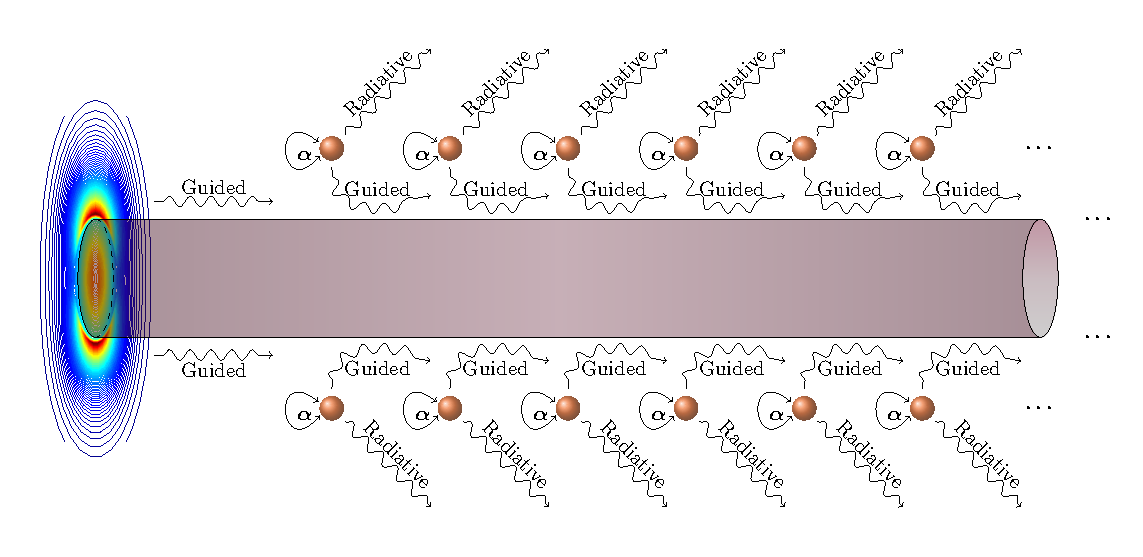
\includegraphics[width=0.85\textwidth]{./Figs/NanofiberTrappedAtoms}}
\caption{Diagram of nanofiber trapped atoms. }
\end{figure}

For our nanofiber case, only $ m=\pm 1 $ $ \text{HE}_{11} $ modes are permitted and guided. We assume the input mode is $ m=+1 $ $ \text{HE}_{11} $ guided mode, which can be written as 
\begin{align}
\mathbf{E}_0(\br,\omega_0)&=E_0 \mathbf{u}^+(r\!_\perp ) e^{i(\beta_0 z+\phi)}, 
\end{align}
where $ \mathbf{u}^{+}(r\!_\perp ) $ denotes the normalized bare nanofiber HE11 transverse mode with forward propagation counterclockwise rotation and circularly polarized light input. Similarly, $ \mathbf{u}^{-}(r\!_\perp ) $ is the forward propagating but clockwise rotating quasi-circular HE11 mode. In general, we denote  $ \mathbf{u}^{\mu}(r\!_\perp ) $ as the normalized $\mu=(\omega,f,p)$ mode radial components, with $ f=\pm $ denoting forward or backward propagating direction, $ p=\pm $ denoting counter-clockwise or clockwise rotation of polarization. For short, we denote $\mathbf{u}^+(r\!_\perp )$ as the forward-propagating and counter-clockwise-rotating $m=1$ guided mode. We also denote $ \beta_0 $ as the eigen wavenumber determined by the fiber eigenvalue  equation. Similarly, we denote $ \mathbf{u}^{\nu}(r\!_\perp ) $ as the radiation mode with mode index $ \nu=(\omega,\beta,m,p) $, where $ m=0,\,\pm 1,\,\pm 2,\cdots $ is the mode index, and $p=\pm$ denotes the polarization pattern. The guided and radiation modes satisfy the orthogonality conditions that 
\begin{align}
\int_0^{2\pi}\mathrm{d}\phi \int_0^\infty n_{r}^2|\mathbf{u}^{(\mu)}(r\!_\perp )|^2r\!_\perp \mathrm{d}r\!_\perp &=1,\\
\int_0^{2\pi}\mathrm{d}\phi \int_0^\infty n_{r}^2\left[\mathbf{u}^{(\nu)}(r\!_\perp )\cdot\mathbf{u}^{(\nu')*}(r\!_\perp )\right]_{\beta=\beta',m=m'}r\!_\perp \mathrm{d}r\!_\perp &=\delta(\omega-\omega')\delta_{pp'}.
\end{align}
The completeness relationships of the modes can be given by
\begin{align}
\sum_{f,p}\int \mathrm{d}\mathbf{k} \,n_r^2\mathbf{u}^{(\mu)}(r\!_\perp )\mathbf{u}^{(\mu)*}(r'\!_\perp ) &= \mathbf{I}\delta^T(r\!_\perp-r'\!_\perp),\\
\sum_{m,p}\int \mathrm{d}\mathbf{k} \, n_r^2\mathbf{u}^{(\nu)}(r\!_\perp )\mathbf{u}^{(\nu)*}(r'\!_\perp ) &=\mathbf{I}\delta^T(r\!_\perp-r'\!_\perp).
\end{align}

As shown in the earlier sections, in general, the output field in presence of a single atom can be written as
\begin{align}
\mathbf{E}(\br) 
&=\mathbf{E}_0(\br)-4\pi k^2\alpha \mathbf{G}(\br,\br')\cdot \mathbf{E}_0(\br')
\end{align}
where we only treat the polarizability as a scalar. The only barrier for solving the output E-field is to solve the dyadic Green function.

In general, there are two strategies to solve the dyadic Green function: one is to solve the dipole emission problem numerically; the other one involves transverse mode decomposition and only needs bare fiber modes. We call the first approach as the \textit{normal} approach, and call the other one as the \textit{approximate} approach. We will describe the two approaches in the successive paragraphs. 

The \textit{normal} approach:

We recall that the equation governs the dyadic Green function can be written as below:
\begin{align}
\left[ -\nabla\times\nabla\times + n^2\frac{\omega^2_0}{c^2} \right] \mathbf{G}(\br,\br') &= \mathbf{I}\delta(\br-\br'),
\end{align}
each column of which can be expressed as
\begin{align}
\left[ -\nabla\times\nabla\times + n^2\frac{\omega^2_0}{c^2} \right] \mathbf{G}_i(\br,\br') &= \mathbf{e}_i\delta(\br-\br'), \label{eq:Gi}
\end{align}
where the subscription $ i=r\!_\perp,\phi,z $ denotes the coordinate components. The $ \mathbf{G}_i(\br,\br') $ in the equation above is the $ i^{th} $ column of the dyadic Green function of $ \mathbf{G}(\br,\br') $. Here, we used $\omega_0$ to indicate the angular frequency of the radiation from the source.  

Comparing Equ.~\eqref{eq:Gi} with Equ.~\eqref{eq:Maxwellwithsource2}, we find that Equ.~\eqref{eq:Gi} is exactly the chromatic wave equation of $ \mathbf{E}(\br) $ when there is a dipole source orientated along $ \mathbf{e}_i $ direction and placed at $ \br' $ with an amplitude of $ -4\pi k^2 $. That is to say that once we solve the electric field components with a unit dipole source orientated along all $ \mathbf{e}_i $ directions, the columns of the dyadic function is just the corresponding field components divided by the factor of $ -4\pi k^2 $. Concretely, in the cylindrical coordinate system, the dyadic Green function elements correspond to the following electric field components emitted by a unit dipole source orientated in the three orthogonal basis:
\begin{equation}
\mathbf{G}(\mathbf{r},\mathbf{r}')=\!\!\!\!\!\!\!\!\!\!\!\!\!\!\!\!\!\!\!\!\!\!\!\! \!\!\!\!\!\!\!\! \!\!\!\!\!\!\!\! \!\!\!\!\!\!\!\!
  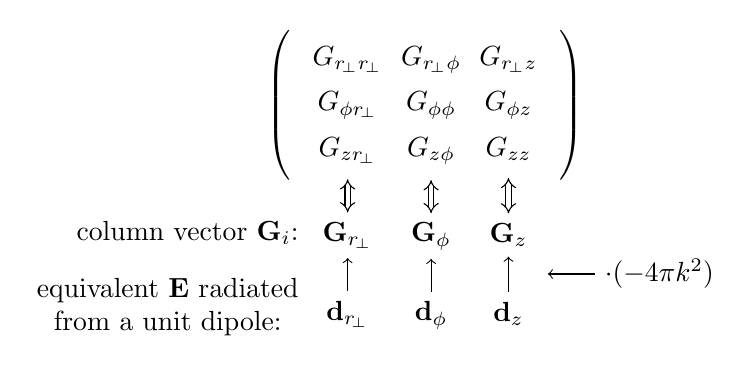
\begin{tikzpicture}[baseline=-\the\dimexpr\fontdimen22\textfont2\relax ]
   \matrix (m)[matrix of math nodes,left delimiter=(,right delimiter=)]
  {
  G_{r\!_\perp r\!_\perp} & G_{r\!_\perp\phi} & G_{r\!_\perp z}\\
  G_{\phi r\!_\perp} & G_{\phi\phi} & G_{\phi z} \\
  G_{zr\!_\perp} & G_{z\phi} & G_{zz} \\
  };
  % Hightlight columns.
  \begin{pgfonlayer}{myback}
    \fhighlight[red!30]{m-1-1}{m-3-1}
    \fhighlight[blue!30]{m-1-2}{m-3-2}
    \fhighlight[green!30]{m-1-3}{m-3-3}
  \end{pgfonlayer}
  % Make links to other equivalent expressions.
  \begin{pgfonlayer}{myback}
    \draw (m-3-1.south)+(-0.5,-0.76) node [left] {column vector $\mathbf{G}_i$:};
    \draw[implies-implies,double equal sign distance] (m-3-1.south)+(0,-0.08) -- +(0,-0.5) node[below]{$ \mathbf{G}_{r\!_\perp} $};
    \draw[implies-implies,double equal sign distance] (m-3-2.south)+(0,-0.08) -- +(0,-0.5) node[below]{$ \mathbf{G}_{\phi} $};
    \draw[implies-implies,double equal sign distance] (m-3-3.south)+(0,-0.1) -- +(0,-0.55) node[below]{$ \mathbf{G}_z $};
    \draw (m-3-1.south)+(-0.5,-1.7) node [left,align=center] {equivalent $ \mathbf{E} $ radiated\\ from a unit dipole:};
    \draw[<-] (m-3-1.south)+(0,-1.08) -- +(0,-1.5) node[below]{$ \mathbf{d}_{r\!_\perp} $};
    \draw[<-] (m-3-2.south)+(0,-1.08) -- +(0,-1.5) node[below]{$ \mathbf{d}_{\phi} $};
    \draw[<-] (m-3-3.south)+(0,-1.1) -- +(0,-1.55) node[below]{$ \mathbf{d}_z $};
    \draw[<-] (m-3-3.south)+(0.5,-1.32) -- +(1.1,-1.32) node[right]{$\cdot (-4\pi k^2)$};
  \end{pgfonlayer}
  \end{tikzpicture}
\end{equation}
%\textcolor{red}{Need to make it look nicely, and continue on...}
The equivalent $ \mathbf{E} $ field has been solved in section~\ref{sec:boundrad} for the radiation problem with one atom.


The \textit{eigenmode decomposition} approach:

In the case that the source is extremely small, the total dyadic Green function should be effectively equal to the transverse dyadic Green function. To illustrate this idea, we can expand the current source of the dipole into transverse and longitudinal parts by
\begin{align}
\mathbf{J}(\br) &= \mathbf{J}_T(\br) + \mathbf{J}_L(\br),
\end{align}
where the transverse and longitudinal current components, $ \mathbf{J}_T(\br) $ and $\mathbf{J}_L(\br)$, satisfy
\begin{align}
\nabla\cdot\mathbf{J}_T (\br) &=0\\
\nabla\times \mathbf{J}_L (\br) &=0.
\end{align}
In SI units, the continuity condition reads
\begin{align}
\nabla\cdot\mathbf{J}=-\pp{}{t}\rho.
\end{align}
Under Coulomb gauge, the transverse and longitudinal currents can then be written as 
\begin{align}
\mathbf{J}_T &= -\frac{1}{\mu_0}(\nabla^2 -\frac{1}{c^2}\spp{}{t})\mathbf{A}\label{eq:Jt_cg}\\
\mathbf{J}_L &= \varepsilon_0 \pp{}{t}\nabla\phi .\label{eq:Jl_cg}
\end{align}
Notice that, the longitudinal current equation (Equ.~\eqref{eq:Jl_cg}) will become purely local for an ideal dipole source, and can be ignored. The longitudinal components may become important for the case with a charged source. Below, we only consider the transverse modes for our analysis.

The Green function for our nanofiber problem satisfies (Equ.~\eqref{eq:dyadicGF})
\begin{align}
\left[ -\nabla\times\nabla\times + n^2k_0^2 \right] \mathbf{G}(\br,\br') &= \mathbf{I}\delta^{(3)}(\br-\br'),
\end{align}
where $n=n(\br\!_\perp)=\sqrt{\varepsilon(\br\!_\perp)}$ and $k_0=\omega_0/c$. Correspondingly, the bare-fiber modes (eigenmodes), $ \mathbf{u}^{(\mu)}(\br) $, satisfy the Maxwell-Helmholtz equation (Equ.~\eqref{MaxwellHelmholtz0}), that is
\begin{align}
[-\nabla\times\nabla\times + n^2(\br)k^2]  \mathbf{u}^{(\mu)}(\br) &=0,
\end{align}
where $ k^2=\frac{\omega_{\mathbf{k}}^2}{c^2} $ and $ \mathbf{k} $ is an arbitrary wave vector.

To use the eigenfunction expansion method to calculate the dyadic Green function, we can define a vector function
\begin{align}
{\mathbf{u}}_\epsilon^{(\mu)}(\br) &= n(\br) \mathbf{u}^{(\mu)}(\br),
\end{align}
which satisfies
\begin{align}
\left[-\frac{1}{n(\br)}\nabla\times\nabla\times \frac{1}{n(\br)} + k^2\right]  {\mathbf{u}}_\epsilon^{(\mu)}(\br) &=0.
\end{align}
Introduced by Glauber and Lewenstein~\cite{Glauber1991}, the operator on the left-hand-side of the equation above, $\mathcal{H}_k = -\frac{1}{n(\br)}\nabla\times\nabla\times \frac{1}{n(\br)} + k^2$, is always Hermitian. Similarly, we can define a Hermitian operator $\mathcal{H}_{k_0} = -\frac{1}{n(\br)}\nabla\times\nabla\times \frac{1}{n(\br)} + k_0^2$, and obtain the eigenequation with $\mathcal{H}_{k_0}$ given by
\begin{align}
\mathcal{H}_{k_0} \mathbf{u}_\epsilon^{(\mu)} &= \lambda_\mu \mathbf{u}_\epsilon^{(\mu)},
\end{align}
which has a set of eigensolutions $ (\mathbf{u}_\epsilon^{(\mu)},\lambda_\mu=k_0^2-k^2) $. There exists a set of adjoint eigensolutions $ (\tilde{\mathbf{u}}_\epsilon^{(\mu)},\lambda_\mu^*) $ to $\mathcal{H}_{k_0}^\dagger \tilde{\mathbf{u}}_\epsilon^{(\mu)} = \lambda_\mu^* \tilde{\mathbf{u}}_\epsilon^{(\mu)}$, such that the biorthogonality relation
\begin{align}
\int \mathbf{u}_\epsilon^{(\mu)} (\br)\cdot \left[\tilde{\mathbf{u}}_\epsilon^{(\mu')}(\br) \right]^* \mathrm{d}\br &= \int n^2(\br) \mathbf{u}^{(\mu)} (\br)\cdot {\mathbf{u}^{(\mu')}}^*(\br) \mathrm{d}\br=\delta_{\mu\mu'},\label{eq:orthutrans}
\end{align}
and the completeness relation
\begin{align}
\sum_\mu \mathbf{u}_\epsilon^{(\mu)} (\br) \left[\tilde{\mathbf{u}}_\epsilon^{(\mu)}(\br') \right]^* &= \sum_\mu n(\br)n(\br') \mathbf{u}^{(\mu)} (\br) {\mathbf{u}^{(\mu)}}^*(\br) =\eye \delta^{(3)}(\br-\br'). 
\end{align}
In our nanofiber case, we can define such a set of mode functions, and in fact we choose them to have the following properties for their adjoint functions:
\begin{align}
\tilde{\mathbf{u}}_\epsilon^{(\mu)}(\br) &= n^*(\br) \tilde{\mathbf{u}}^{(\mu)}(\br)\\
\tilde{\mathbf{u}}^{(\mu)}(\br) &= {\mathbf{u}^{(\tilde{\mu})}}^*(\br)\\
{\mathbf{u}^{(\tilde{\mu})}}(\br) &= {\mathbf{u}^{(\mu)}}^*(\br)
\end{align}
with $ \tilde{\mu}=(\omega_0,-m,-f) $. For a single-mode nanofiber, we let $ n(\br)=n(\br\!_\perp) $ be real and define $ \mathbf{u}^{(\mu)}(\br)=\mathbf{u}_{mf}(r\!_\perp )e^{if\beta z+im\phi} $ for the guided $\mathrm{HE}_{11}$ modes with a propagation constant $ \beta  $. The completeness relation for the normalized modes will yield a transverse $ \delta $-function, $ \delta^T(\br-\br') $, having the property that
\begin{align}
\mathbf{f}^T(\br')&=\int \mathrm{d}\br\,\, \delta^T(\br-\br')\mathbf{f}(\br).
\end{align} 
Similar to the integration in the general biorthogonality relationship, if we only integrate over the transverse plane of a mode, we will obtain
\begin{align}
\int_0^{2\pi}\!\!\!\!\! \mathrm{d}\phi\!\! \int_0^\infty\!\!\!\! r\!_\perp \mathrm{d}r\!_\perp  n^2(r\!_\perp) \mathbf{u}_{mf}(r\!_\perp )\!\cdot\!\mathbf{u}_{m'f'}^*(r\!_\perp )& e^{i(f\!-\!f')\beta z+i(m\! -\! m')\phi}  =\delta_{mm'}e^{i(f\!-\!f')\beta z} \label{eq:orthutrans2D}.
\end{align}


From those eigensolutions, we can define a dyad, $ \mathbf{G}_\epsilon(\br,\br') $, satisfying
\begin{align}
\mathbf{G}_\epsilon(\br,\br') &= n(\br) \mathbf{G}(\br,\br') n(\br'),\\
\mathcal{H}_{k_0} \mathbf{G}_\epsilon(\br,\br') &= \mathbf{I}\delta^{(3)}(\br-\br').\label{eq:HGtilde}
\end{align}

One can expand the dyadic function $ \mathbf{G}_\epsilon(\br,\br') $ in terms of the transverse eigenmodes by
\begin{align}
\mathbf{G}_\epsilon(\br,\br')\approx\mathbf{G}_\epsilon^T(\br,\br')= \sum_{\mu} \mathbf{u}_\epsilon^{(\mu)}(\br) \mathbf{A}_\epsilon^{(\mu)}(\br'), \label{eq:transGappr}
\end{align}
where the coefficient vector $\mathbf{A}_\epsilon^{(\mu)}(\br')  $ does not depend on $ \br $.
Substituting Equ.~\eqref{eq:transGappr} into Equ.~\eqref{eq:HGtilde}, we obtain
\begin{align}
\sum_{\mathbf{k}} \left[ \mathcal{H}_{k_0}  \mathbf{u}_\epsilon^{(\mu)}(\br)\right] \mathbf{A}_\epsilon^{(\mu)}(\br') &= \mathbf{I}\delta^{(3)}(\br-\br')\\
\Leftrightarrow \sum_\mu (k_0^2-k^2) \mathbf{u}_\epsilon^{(\mu)}(\br) \mathbf{A}_\epsilon^{(\mu)}(\br') &= \mathbf{I}\delta^{(3)}(\br-\br') = \sum_{\mu} \mathbf{u}_\epsilon^{(\mu)}(\mathbf{r} )\left[\tilde{\mathbf{u}}_\epsilon^{(\mu)}(\mathbf{r}^\prime )\right]^*.
\end{align}
Therefore, we can solve the coefficient vector for an arbitrary eigenmode to give
\begin{align}
\mathbf{A}_\epsilon^{(\mu)}(\br') &= \frac{c^2 \left[ \tilde{\mathbf{u}}_\epsilon^{(\mu)}(\br')\right]^*}{\omega_0^2-\omega_{\mathbf{k}}^2}.
\end{align}
Hence, 
\begin{align}
\mathbf{G}_\epsilon(\br,\br')= \sum_{\mu} \frac{c^2\mathbf{u}_\epsilon^{(\mu)}(\br)\left[\tilde{\mathbf{u}}_\epsilon^{(\mu)}(\br')\right]^*}{\omega_0^2-\omega_{\mathbf{k}}^2} = n(\br) \left[\sum_{\mu} \frac{c^2 {\mathbf{u}}^{(\mu)}(\br) {\mathbf{u}^{(\mu)}}^*(\br')}{\omega_0^2-\omega_{\mathbf{k}}^2} \right]n(\br').
\end{align}
By the definition of $\mathbf{G}_\epsilon(\br,\br')  $, the dyadic Green function can be written by 
\begin{align}
\mathbf{G}(\br,\br')\approx \sum_{\mu} \frac{c^2\mathbf{u}^{(\mu)}(\br) {\mathbf{u}^{(\mu)}}^*(\br')}{\omega_0^2-\omega_{\mathbf{k}}^2}.
\end{align}
For the guided $\mathrm{HE}_{11}$ modes, we have 
\begin{align}
\mathbf{G}^g(\br,\br') &= \sum_{\beta,m,f=\pm 1} \frac{c^2\mathbf{u}_{\mu}(r\!_\perp)\mathbf{u}^*_{\mu}(r_{\!\perp}^\prime)}{\omega_0^2-\omega_\beta^2}e^{if\beta(z-z')+im(\phi-\phi')},\label{eq:Gganaly}
\end{align}
where $ \omega_\beta $ is the angular frequency of the guided HE11 modes with the amplitude $ z $-component of the wave vector being $ \beta $. \textcolor{red}{The mode index should be $ \mu=(\beta_0,m=\pm 1,f=\pm 1) $. This notation should be unified starting here.} Now, we can use the dispersion expansion of $ \omega_\beta $ around $ \omega_0 $ with a group velocity $ v_g $ that 
\begin{align}
\omega_\beta &=\omega_0 + \dd{\omega_\beta}{\beta}(\beta-f\beta_0) +\cdots = \omega_0 + fv_g(\beta-f\beta_0) +\cdots\\
\Rightarrow \omega_\beta - \omega_0 &= fv_g(\beta-f\beta_0) +\cdots
\end{align}
Meanwhile, the sum over the mode index can be written as an integral over $ \beta $:
\begin{align}
\sum_{\beta} \Leftrightarrow & \frac{L}{2\pi} \int_{-\infty}^{\infty} \mathrm{d}\beta, \quad \text{if $\beta$ includes the propagation direction},\\
\quad \mathrm{or}\quad &\frac{L}{2\pi}\sum_{f=\pm 1} \int_0^{\infty} \mathrm{d}\beta,\quad\text{if the propagation direction is separated out}.
\end{align}
This  transformation comes from the consideration that, in the continuous limit, the propagating guided wave is periodic within the quantization length period $ L $ and the periodicity condition is that $ \beta_n L=2\pi n $, where $ n=1,\,2,\,\ldots $. Hence, the dyadic Green function for the guided modes (Equ.~\eqref{eq:Gganaly}) can be written as
\begin{align}
\!\!\!\!\!\!\!\!\! \mathbf{G}^g(\br,\br') &= \frac{L}{2\pi}\sum_{m,f=\pm 1}\int_0^\infty \mathrm{d}\beta \frac{c^2\mathbf{u}_{m}(r\!_\perp)\mathbf{u}^*_{m}(r_{\!\perp}^\prime)}{\omega_0^2-\omega_\beta^2}e^{if\beta(z-z')+im(\phi-\phi')}\\
&= -\frac{c^2 L}{2\pi}\!\!\sum_{m,f=\pm 1}\int_0^\infty\!\! \mathrm{d}\omega_\beta \frac{\mathrm{d}\beta}{\mathrm{d}\omega_\beta} \frac{\mathbf{u}_{m}(r\!_\perp)\mathbf{u}^*_{m}(r_{\!\perp}^\prime)}{(\omega_0\! +\!\omega_\beta) (\omega_0\!-\!\omega_\beta)} e^{i\!f\!\beta(z\!-\!z')+im(\phi\!-\!\phi')}\label{eq:eigGFintegral}\\
&\approx -\frac{c^2L}{2\pi} \!\!\! \sum_{m,f=\pm 1}\!\!\!\!\! \pi i\,\!  \frac{f}{fv_g} \mathrm{Res}\!\! \left[\! \frac{\mathbf{u}_{m}\!(r\!_\perp\! ) \mathbf{u}^*_{m}\! (r_{\!\perp}^\prime\! ) e^{i\! f\! \beta(z \!-\! z')+im(\phi\!-\! \phi')} }{(\omega_0+\omega_\beta)(\omega_0-\omega_\beta)} \!\right]\!\!\!\!_{\begin{array}{l} \omega_\beta\! =\!\omega_0 \\ \beta\! =\!\beta_0\end{array} }\\
&= -\frac{ic^2L}{4\omega_0v_g} \sum_{m,f=\pm 1} \mathbf{u}_{m}(r\!_\perp)\mathbf{u}^*_{m}(r_{\!\perp}^\prime)e^{if\beta_0(z-z')+im(\phi-\phi')},
\end{align}
where $ \beta_0 $ is the propagation constant with a given $ \omega_0 $ for the input/emission field. The integral path and the equivalence to the residue at $ \beta_0 $ is illustrated in part (c) of Fig.(\ref{fig:integralpaths}). We have used the fact that $ \int_{0-if\epsilon}^{\infty-if\epsilon} \mathrm{\omega_\beta}g(\omega_\beta) = P\left[ g(\omega_\beta)\right] +f\pi i \mathrm{Res}\left[g(\omega_\beta) \right] $, and ignored the principal value integral part, $ P\left[ g(\omega_\beta)\right] $. The principal value part yields the level shift of the atom due to the fiber modes, which should be negligible in the dispersive regime we are considering about. \todo[inline]{Note: the figure of integral path needs to be changed to have integrals always from $0$ to $\infty$ for $\omega_\beta$ and choose the shift of the integral path based on the sign of $f(z-z')$.} 

By using the relation that 
\begin{align}
k_0 &=\frac{\omega_0}{c}\\
n_g&=\sqrt{\varepsilon_g}= \frac{c}{v_g}
\end{align}
the dyadic Green function for the guided modes can also be written as
\begin{align}
\mathbf{G}^g(\br,\br') &\approx -\frac{in_gL}{4k_0} \sum_{m,f=\pm 1} \mathbf{u}_{m}(r\!_\perp)\mathbf{u}^*_{m}(r_{\!\perp}^\prime)e^{if\beta_0(z-z')+im(\phi-\phi')}.
\end{align}
We make $ L=1 $ for now, which should be canceled through multiplying with the quantization factor. 
 


The numerical comparison of the two approaches has been done and confirmed that these two approaches match up really well as long as we treat the integration paths under the same physics scenario.  

\begin{figure}
\centering\makebox[\textwidth]{
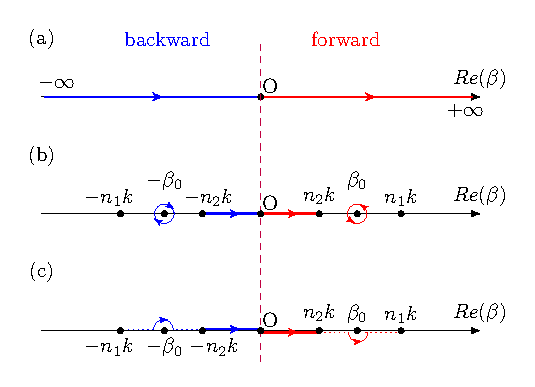
\includegraphics[width=0.85\textwidth]{./Figs/integratepath_GF}}
\caption{Integral paths for the dyadic Green function calculations. Part (a) is the integral path for the dipole's free-space field contribution calculation (see, for example, Equ.~\eqref{ET0RC1}). Part (b) is the integral path for the reflected and transmitted field contributions calculation (see, for example, Equ.~\eqref{ET0RC1}). Part (c) is the integral path for the dyadic Green function calculation using the eigenmode decomposition method (see Equ.~\eqref{eq:eigGFintegral}). The integral paths on the left-hand-side (in blue) indicate the backward propagating contributions, while the right-hand-side (in red) parts corresponding to the forward propagating contributions. For the eigenmode decomposition method in part (c), if one choose to use $ f=\pm 1 $ to indicate the propagation direction, then only the $ \beta>0 $ portion of integral path will be applied. }
\label{fig:integralpaths}
\end{figure}

As shown in an earlier section, the guided and radiation modes contribution to the dyadic Green function can be identified through the specific choice of integral paths. In Fig.~\ref{fig:integralpaths}, part (a) shows the integral path to calculate the dipole free-space contribution which does not yield guided mode contribution to the total dyadic Green function. Part (b) of the figure shows the loop and real-valued integral paths of the guided and radiation mode divisions to the reflected and transmitted field components. The $ \mathrm{Re}(\beta)<0 $ and $ \mathrm{Re}(\beta)>0 $ parts correspond to the backward and forward propagating contributions, respectively. Part (c) of the figure indicates the integral path using the eigenmode decomposition method in the case that the sign of $ \mathrm{Re}(\beta) $ indicates the propagation directions. Depending on the propagation directions, we should choose the right integral paths for the corresponding methods adopted, and different methods should yield the same result. 

For the decay rate calculation, both forward and backward propagation contributions should be averaged, or just include one direction.  


\subsection{Calculation of group velocity and group index of refraction ($ v_g $ and $ n_g $)}
For a guided mode in a waveguide, the phase index of refraction is defined as
\begin{align}
n_p &= \frac{\beta}{k}.
\end{align}
Correspondingly, the group velocity and group index of refraction for a guided mode in a waveguide can be given by
\begin{align}
v_g &= \dd{\omega}{\beta},\\
n_g &= \frac{c}{v_g}=\dd{\beta}{k}.
\end{align}
Therefore, the group velocity and group index of refraction of the $ HE_{11} $ mode can calculated from the eigen function of $ \beta $ (see Appendix A of Ref.~\cite{LeKien2005}). 

In general, the eigen function of $ \beta $ can be expressed as
\begin{align}
f(h,q,k,\beta) &=0
\end{align}
with $ h $ and $ q $ are both functions of $ k $ and $ \beta $. 
We differentiate the equation above with respect to $ \beta $ on both sides, and obtain
\begin{align}
\dd{f}{\beta} &= \pp{f}{h} \left(\pp{h}{k}\dd{k}{\beta}+\pp{h}{\beta} \right) + \pp{f}{q}\left(\pp{q}{k}\dd{k}{\beta}+\pp{q}{\beta} \right) +\pp{f}{k}\dd{k}{\beta}+\pp{f}{\beta}=0\\
\Rightarrow & \left( \pp{f}{h}\pp{h}{k}+\pp{f}{q}\pp{q}{k}+\pp{f}{k} \right)\dd{k}{\beta} = -\left(\pp{f}{h}\pp{h}{\beta}+\pp{f}{q}\pp{q}{\beta}+\pp{f}{\beta} \right)
\end{align}
\begin{align}
\Rightarrow &\quad\quad n_g = \dd{\beta}{k} = -\frac{\pp{f}{h}\pp{h}{k}+\pp{f}{q}\pp{q}{k}+\pp{f}{k}}
{\pp{f}{h}\pp{h}{\beta}+\pp{f}{q}\pp{q}{\beta}+\pp{f}{\beta}}.
\end{align}

Physically, the group index of refraction indicates the waveguide dispersion for a given propagating mode. Here, we can ignore the material dispersion due to the small response delay of the silica molecules of the waveguide substrate. Since the waveguide dispersion is merely a property of the waveguide, the presence of the radiating atom does not affect the group index of refraction at all (have checked numerically through solving the eigen function of $ \beta $ in presence of an atom). 

From the perspective of energy flowing, the group velocity can also be given by
\begin{align}
v_g&=\frac{P}{W}.
\end{align}
The physics interpretation of group and phase velocity of a waveguide mode can be found in the notes on \textit{Group velocity of the nanofiber}. The effective zig-zag ray model is also described in the notes for understanding the mechanism of group and phase index of refractions. For our nanofiber case, the $ D_2 $ transition line of Cs atoms does not have a strong enhancement of group index of refraction for the guided mode, compared to the phase index of refraction. The $ D_1 $ line has a relatively strong enhancement of group index since the wave can penetrate into the clad much deeper compared to the $ D_2 $ line case. 

\section{Phase shift and polarizability transformation}
Using the results for the dyadic Green function of the guided modes, one can write the output electric field due to the guided modes (from Equ.~\eqref{eq:EoutG}) as 
\begin{align}
\mathbf{E}(\br) & = \mathbf{E}_0(\br) -4\pi k_0^2 \alpha \mathbf{G}^g(\br,\br')\cdot\mathbf{E}_0(\br'),
\end{align}
where the polarizability has been treated as a scalar. The field at the position of the atom is then
\begin{align}
\mathbf{E}(\br') &= \left[\eye-4\pi k_0^2 \alpha \mathbf{G}^g(\br',\br')\right]\cdot\mathbf{E}_0(\br').
%&\approx \exp\left[-4\pi k^2 \alpha \mathbf{G}^g(\br',\br')\right]\cdot\mathbf{E}_0(\br').
\end{align}

As a concrete example, we can consider the case that $ z'=0 $ and $ \phi'=0 $ for the atom, and the input field is the $ m=+1,\,f=+1 $ HE11 forward propagating mode that
\begin{align}
\mathbf{E}_0(\br) &= E_0n_{e\!f\!f} \mathbf{u}_{m=1}^{f=1} (\br) = E_0n_{e\!f\!f} \mathbf{u}_1^1 (\mathbf{r}\!_\perp)e^{i\phi+i\beta_0 z}. 
\end{align}
The output field in the forward direction at $ z\ge 0 $ \textcolor{red}{can then be expressed by}
\begin{align}
\mathbf{E}(\br) &= E_0n_{e\!f\!f}\mathbf{u}_{1}^{1} (\br) + \sum_{m,f=\pm 1} C_{mf} E_0n_{e\!f\!f} \mathbf{u}_m^f(\br),  
\end{align}
where the projection coefficients are 
\begin{align}
C_{mf} &= -4\pi k_0^2 \alpha \!\int\! \mathrm{d}^2r\!_\perp n^2_{e\!f\!f} {\mathbf{u}^f_m}^*(\mathbf{r},z)\cdot \mathbf{G}^g(\br,\br') \!\cdot\! \mathbf{u}_1^1(\mathbf{r}^\prime,z')\\
&= -4\pi k_0^2 \alpha \!\int\! \mathrm{d}^2r\!_\perp n^2_{e\!f\!f} {\mathbf{u}^f_m}^*(\mathbf{r}\!_\perp)\cdot \mathbf{G}^g(\br,\br') \!\cdot\! \mathbf{u}_1^1(\mathbf{r}^\prime\!_\perp)\\
&= -4\pi k_0^2 \alpha \!\int\! \mathrm{d}^2r\!_\perp n^2_{e\!f\!f} {\mathbf{u}^f_m}^{\!\!*}(r\!_\perp)\!\cdot\! \mathbf{G}^g(\br,\br') \!\cdot\! \mathbf{u}_1^1(r^\prime\!\!_\perp)e^{i\beta_0(z'-fz)+i(\phi'-m\phi)}.
\end{align}
Using the transverse mode approximation of the dyadic Green function, these coefficients become
\begin{align}
C_{mf} &= i\pi k_0 n_g\alpha \!\int\! \mathrm{d}^2r\!_\perp n^2_{e\!f\!f} {\mathbf{u}^f_m}^*(\mathbf{r}\!_\perp)\cdot\!\!\!\!\!\! \sum_{f',m'=\pm 1}\!\!\!\! \left[\mathbf{u}_{m'}^{f'}(\mathbf{r}\!_\perp){\mathbf{u}^{f'}_{m'}}^*(\mathbf{r}^\prime\!_\perp) \right]\!\cdot\! \mathbf{u}_1^1(\mathbf{r}^\prime\!_\perp)\nonumber\\
&\quad\quad\quad e^{if'\beta_0(z-z')} e^{i\beta_0(z'-fz)}\\
&= i\pi k_0 n_g\alpha  {\mathbf{u}^f_m}^*(r'_{\!\perp})\cdot \mathbf{u}_1^1(r'_{\!\perp})e^{i\beta_0 (1-f)z'+i(1-m)\phi'}.
\end{align}
Notice that, the phase factor in the exponential part depends on the position of the atom as well as the mode index $ (m,f) $. If $ m,f\neq 1 $, there will be a fast beating term in the projection coefficient, and may be averaged out in some cases. If the atom is positioned at $ \phi'=0 $ and $ z'=0 $ line, and then the phase factor part will vanish. 
%The projection coefficients can be written as 
%\begin{align}
%C_{mf} &\approx C_m\equiv  i\pi k_0 n_g\alpha  \mathbf{u}^*_m(\br'_{\!\perp})\cdot \mathbf{u}_1(\br'_{\!\perp})\\
%&= i\pi k_0 n_g\alpha  \mathbf{u}^*_m(r'_{\!\perp})\cdot \mathbf{u}_1(r'_{\!\perp})e^{i(1-m)\phi'}.
%\end{align}

Therefore, the emerged forwarding $ m=-1 $ mode has an amplitude 
\begin{align}
C_{-+}=i\pi k_0 n_g\alpha  {\mathbf{u}^1_{-1}}^*(r'_{\!\perp})\cdot \mathbf{u}_1^1(r'_{\!\perp})e^{i2\phi'}.
\end{align}
Similarly, the backwarding $ m=1 $ and $ m=-1 $ modes have amplitudes 
\begin{align}
C_{+-} &=i\pi k_0 n_g\alpha  {\mathbf{u}^{-1}_1}^*(r'_{\!\perp})\cdot \mathbf{u}_1^1(r'_{\!\perp})e^{i2\beta_0 z'}\\
C_{--} &=i\pi k_0 n_g\alpha  {\mathbf{u}^{-1}_{-1}}^*(r'_{\!\perp})\cdot \mathbf{u}_1^1(r'_{\!\perp})e^{i2\beta_0 z'+i2\phi'}.
\end{align}

The output $ m=1 $ HE11 mode component in presence of the atom in the forward direction is then given by
\begin{align}
\mathbf{E}_+(\br) &= (1+C_{11})E_0n_{e\!f\!f}\mathbf{u}_{1}^{1} (\br)\\
&=\left[1 +i\pi k_0 n_g\alpha  | \mathbf{u}_1^1(r'_{\!\perp})|^2 \right] E_0n_{e\!f\!f}\mathbf{u}_{1}^{1} (\br)\\
&\approx \exp\left[i\pi k_0 n_g\alpha  | \mathbf{u}_1^1(r'_{\!\perp})|^2 \right] E_0n_{e\!f\!f}\mathbf{u}_{1}^{1} (\br)\\
&= te^{i\delta\phi}E_0n_{e\!f\!f}\mathbf{u}_{1}^{1} (\br), 
\end{align}
where the factor change of the mode's amplitude is 
\begin{align}
t=\exp\left[\Im[C_{11}]\right]=\exp\left[ -\pi k_0 n_g \Im[\alpha]  | \mathbf{u}_1^1(r'_{\!\perp})|^2 \right]
\end{align}
and the phase shift is
\begin{align}
\delta\phi &= \Re[C_{11}]\\
&=\pi k_0 n_g\Re[\alpha]  | \mathbf{u}_1^1(r'_{\!\perp})|^2\\
&= \pi \Re[\alpha] \frac{\omega_0}{v_g}  | \mathbf{u}_1^1(r'_{\!\perp})|^2\\
&= \pi \Re[\alpha] \frac{\omega_0}{v_gA'_{e\!f\!f}},
\end{align}
where the symbols $ \Im[\cdot] $ and $ \Re[\cdot] $ indicate the imaginary and real parts of the variable inside; the effective area at the atom position defined as $ A'_{e\!f\!f}=1/| \mathbf{u}_1^1(r'_{\!\perp})|^2 $. 

We can see that the attenuation of the mode comes from the state decay of the dipole source. If we use the definition of the polarizability and scattering rate of the dipole that 
\begin{align}
\alpha &=-\frac{|d_{eg}|^2}{\hbar \Delta}, \,\, (\Delta=\omega_{\mathbf{k}}-\omega_{eg}=\omega-\omega_0)\\
\Gamma^{1D}_{p,f} &= \gamma^g=2\pi \frac{|d_{eg}|^2}{\hbar A'_{e\!f\!f}}\left(\frac{\omega_0}{v_g} \right)
\end{align}
we find that 
\begin{align}\label{phaseshiftGamma1D}
\delta\phi &= -\pi \frac{|d_{eg}|^2}{\hbar \Delta} \frac{\omega_0}{v_gA'_{e\!f\!f}}=-\frac{\Gamma^{1\!D}_{p,f}}{2\Delta}.
\end{align}
The subscript $ p $ indicates polarization, and $ f $ indicates propagation direction. \textcolor{red}{Check the factor of 2 below.}

%\textcolor{red}{This result has the same form as Ivan's result derived from Heisenberg picture, except that I used $ \omega_0=\omega_{eg} $ to define the scattering rate rather than explicitly using $ \omega_{eg} $ to define the decay rate in Ivan's result. }

Using the relationships that 
\begin{align}
\Gamma_{vac} &= \frac{4}{3} \left( \frac{\omega_0}{c}\right)^3 \frac{|d_{eg}|^2}{\hbar}\\
\Rightarrow \frac{\Gamma^{1\!D}_{p,f}}{\Gamma_{vac}} &= \frac{3\pi}{2k_0^2A'_{e\!f\!f}} \frac{c}{v_g} = \frac{1}{4} \frac{c}{v_g} \frac{\sigma_0}{A'_{e\!f\!f}},\\
\sigma_0 &= \frac{3\lambda^2}{2\pi} \equiv \text{resonant cross section}
\end{align}
the 1-dimensional scattering rate can be written as 
\begin{align}\label{Gamma1DGammavac}
\Gamma^{1\!D}_{p,f} &= \frac{1}{4} \frac{c}{v_g} \frac{\sigma_0}{A'_{e\!f\!f}}\Gamma_{vac}.
\end{align}
The phase shift is then
\begin{align}
\delta\phi &= -\frac{\Gamma^{1\!D}_{p,f}}{2\Delta} = -\frac{c}{v_g} \frac{\sigma_0 }{A'_{e\!f\!f}} \frac{\Gamma_{vac}}{8\Delta} = -\frac{c}{v_g} \sigma_0 |\mathbf{u}_1^1 (r'_{\!\perp})|^2 \frac{\Gamma_{vac}}{8\Delta}.
\end{align}

\bigskip
\textbf{Field goes into the opposite rotating mode:}

Similarly, the field goes into the forward propagating $ m=-1 $ HE11 mode has the form of 
\begin{align}
\mathbf{E}_{-}(\br) &=  i\pi k_0 n_{e\!f\!f}\alpha  \mathbf{u}^*_{-1}(r'_{\!\perp})\cdot \mathbf{u}_1(r'_{\!\perp})e^{i2\phi'}E_0n_{e\!f\!f}\mathbf{u}_{-1}^1(\br).
\end{align}
$ \mathbf{E}_{+}(\br) $ and $\mathbf{E}_{-}(\br)$ defines the transformation of polarization of the light. 

\bigskip
\textbf{The rotation angle on the Poincare sphere:}

If we launch two equal-power yet orthogonal quasi-linear modes, H and V, and let the atom sit along the major axis of the H mode, the atom will feel both modes in different strengths. Equivalently, we can also launch a linearly polarized light bisect the angle between the $ x $- and $ y $-axes, and let the atom sit along the $ x $-axis. The rotation angle on the Poincare sphere can be given by
\begin{align}
\varphi &= \delta\phi_H-\delta\phi_V= \pi \frac{\omega_0}{v_g} \Re[\alpha] \left[| \mathbf{u}_H(r'_{\!\perp})|^2- | \mathbf{u}_V(r'_{\!\perp})|^2 \right]\\
&= \sigma_0\frac{c}{v_g}\frac{\Gamma_{vac}}{8\Delta}\left[| \mathbf{u}_H(r'_{\!\perp})|^2- | \mathbf{u}_V(r'_{\!\perp})|^2 \right].\label{eq:Faradayrotang}
\end{align}

%\textcolor{red}{Diagrams for the configuration of setups...}
\begin{figure}
\centering\makebox[\textwidth]{
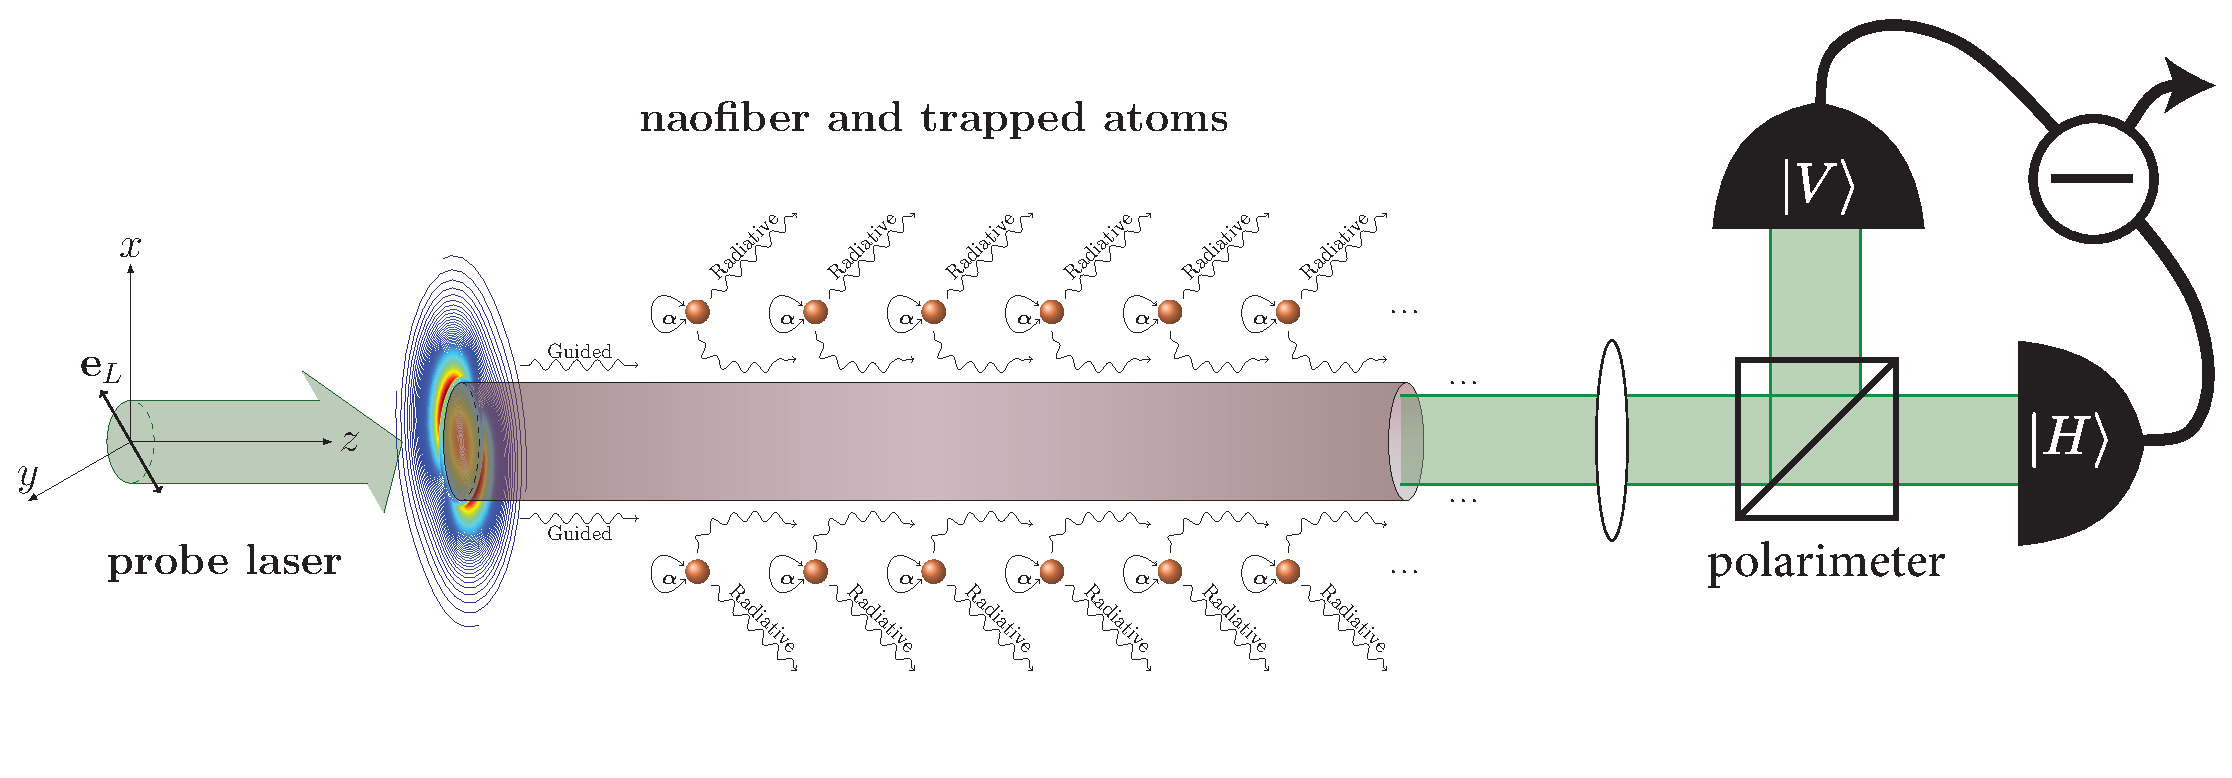
\includegraphics[width=12cm]{./Figs/BirefringenceMeasurement}}
\caption{Setup diagram for birefringence measurement.}
\end{figure}

\begin{figure}
\centering\makebox[\textwidth]{
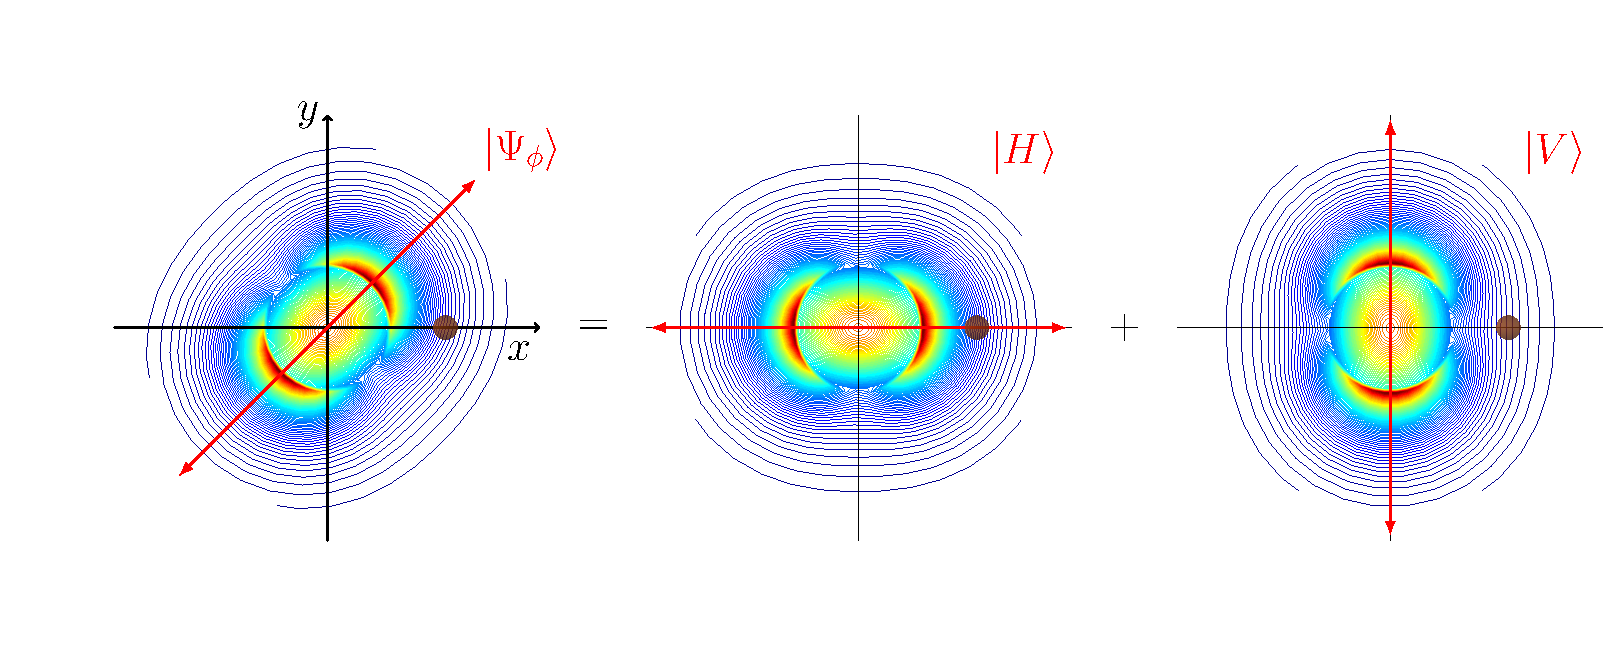
\includegraphics[width=12cm]{./Figs/Modes_Rot45HV}}
\caption{Mode decomposition of an input quasilinear polarized laser beam. The input beam is polarized along the bisection between $ x $- and $ y $-axes. It is equivalent to have one $ |H\rangle $ mode and one $ |V\rangle $ mode with input polarized along the $ x $-axis and $ y $-axis, respectively.}
\end{figure}

\begin{figure}
\centering\makebox[\textwidth]{
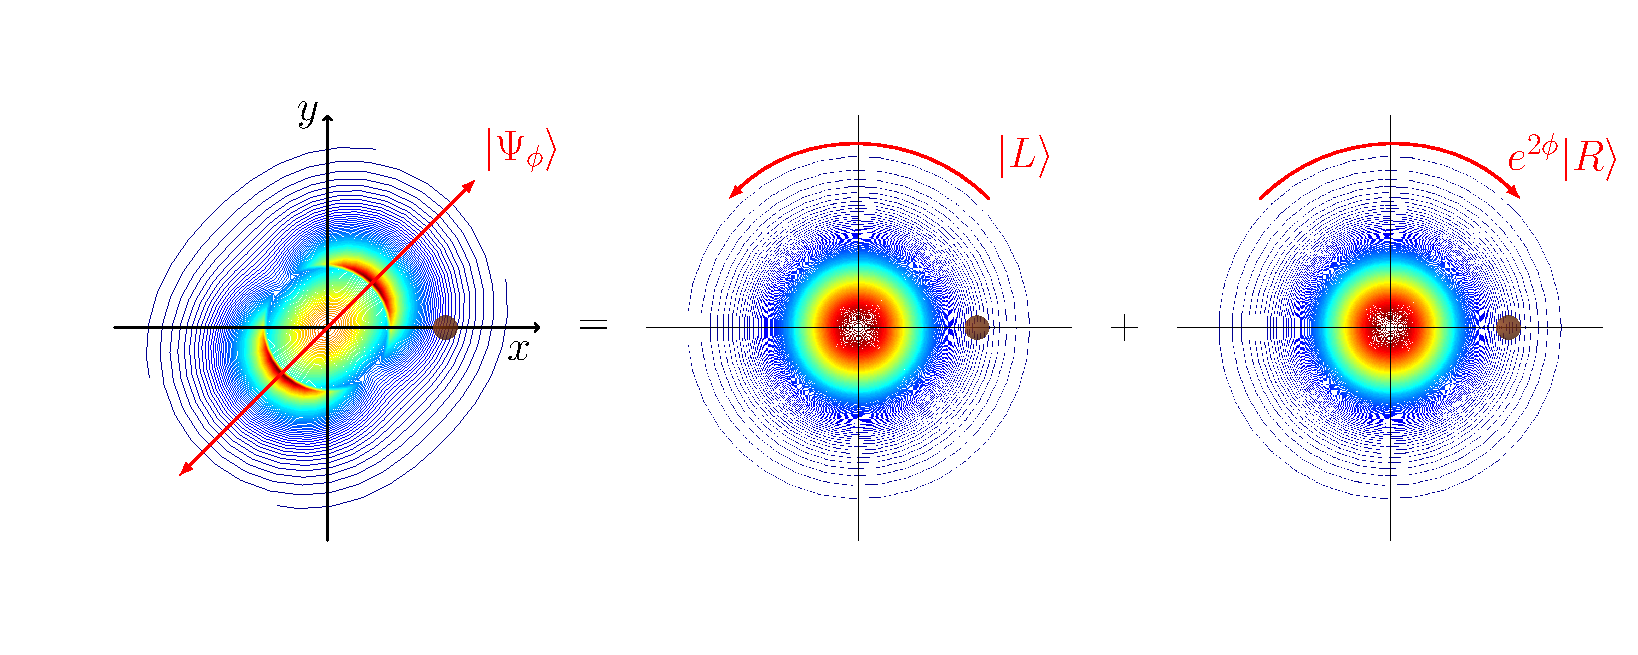
\includegraphics[width=12cm]{./Figs/Modes_Rot45LR}}
\caption{Mode decomposition of an input quasilinear polarized laser beam. The input beam is polarized along the bisection between $ x $- and $ y $-axes. It is equivalent to have one $ |L\rangle $ mode and one $ |R\rangle $ mode with input circularly polarized light rotating counter-clockwise and clockwise, respectively.}
\end{figure}

\bigskip
\textbf{Comparison to the vacuum case:}

Notice that, the phase shift for an atom in vacuum can be given in a similar form by
\begin{align}
\delta\phi^{vac} &= 2\pi \frac{\omega_0}{cA} \Re[\alpha] |\mathbf{u}_{00}(\br')|^2 =  2\pi \frac{\omega_0}{c A^{vac'}_{e\!f\!f}} \Re[\alpha]=-\frac{1}{A} \sigma_0 |\mathbf{u}_{00} (r'_{\!\perp})|^2 \frac{\Gamma_{vac}}{4\Delta},
\end{align}
where $\mathbf{u}_{00}(\br')  $ is the TEM00 mode of a Gaussian laser field at the atom position, $ A=\frac{\pi W_0^2}{2} $ is the mode area of the Gaussian beam with wist $ W_0 $. Hence, the relative strength of phase shift due to the presence of a nanofiber versus vacuum can be given by
\begin{align}
\frac{\delta\phi^{nano}}{\delta\phi^{vac}} &=\frac{A_{e\!f\!f}^{vac'}}{A_{e\!f\!f}^{11}}= \frac{A}{2} \!n_g\! \frac{|\mathbf{u}_1(r_\perp^{nano'})|^2}{|\mathbf{u}_{00}(r_\perp^{vac'})|^2}.
\end{align}
In the vacuum case, the strongest mode is given by $ |\mathbf{u}_{00}(r_\perp^{vac'})|=1 $ when the atom is placed at the center of the beam waist. 

\section{Resolution of birefringence spectroscopy measurement for the nanofiber trapped atom system}\label{sec:birefringenceresolution}
The Faraday spectroscopy theory for optical lattice has been published in Ref.~\cite{Smith2003a}. Following this thread, we present the birefringence spectroscopy analysis for our nanofiber case.

To measure the Stocks vector rotation angle on the Poincare sphere, that is the transformation of the polarization of the light, we launch a probe light along the bisection line between $ x $- and $ y $-axes, and trap the atom on the $ x $-axis, and then measure the output powers of the counterclockwise-rotating ($ \sigma_+ $) and the clockwise-rotating ($ \sigma_- $) components of the output. From Equ.~\eqref{eq:Faradayrotang}, the total differential phase shift between the $ \sigma_+ $ and $ \sigma_- $ components of the probed traveling light interacted with $ N $ atoms can be given by
\begin{align}
\varphi_{_N} &= N\sigma_0\frac{c}{v_g}\frac{\Gamma_{vac}}{4\Delta}\left[| \mathbf{u}_H(r'_{\!\perp})|^2- | \mathbf{u}_V(r'_{\!\perp})|^2 \right].
\end{align}
\textcolor{red}{(Note: there may be a factor of 2 in the equation above and below. Needs to check.)}
The transformation of polarization is measured in terms of the total power difference between the $ x $- and $ y $-components of the field. The measured signal power is given by
\begin{align}
\Delta P_S &= P_0 \sin(\varphi_{_N}) \approx P_0 \varphi_{_N}. \label{eq:polsignal}
\end{align}

\textcolor{red}{Diagram of the experimental setup...}

Our resolution of detection is limited by the shot noise characterized by the fluctuations in the power difference with a root mean square amplitude of 
\begin{align}
\Delta P_{SN} &= \sqrt{\frac{P_0 \hbar \omega_0 }{2\kappa \tau_{pd}}}. \label{eq:shotnoise}
\end{align}
In the extreme case that the signal is equal to the noise, that is to make $ \Delta P_S=\Delta P_{SN} $, we can obtain the minimum number of atoms that we can detect (the resolution) as
\begin{align}
N_{min} &= \sqrt{\frac{8  \hbar \omega_0  }{P_0\kappa \tau_{pd}}}\frac{\Delta}{\sigma_0 n_g\Gamma_{vac}}\frac{1}{\left[| \mathbf{u}_H(r'_{\!\perp})|^2- | \mathbf{u}_V(r'_{\!\perp})|^2 \right]}\\
&=\sqrt{\frac{8  \hbar \omega_0  }{P_0\kappa \tau_{pd}}}\frac{2\pi\Delta}{3\lambda^2 \frac{4}{3} \left( \frac{\omega_0}{c}\right)^3 \frac{|d_{eg}|^2}{\hbar}}\frac{A_{e\!f\!f}^V}{\zeta -1 }\\
&= \sqrt{\frac{\hbar^3 \pi c  }{P_0\kappa \tau_{pd}\lambda}}\frac{\lambda\Delta }{  \left( 2\pi\right)^2 |d_{eg}|^2}\frac{A_{e\!f\!f}^V}{\zeta -1 }\\
&= \frac{1}{4\pi}\sqrt{\frac{\hbar^3 c \lambda }{\pi P_0\kappa \tau_{pd}}}\frac{\Delta }{   |d_{eg}|^2}\frac{A_{e\!f\!f}^V}{\zeta -1 },
\end{align}
with
\begin{align}
A_{e\!f\!f}^V &= \frac{1}{n_g| \mathbf{u}_V(r'_{\!\perp})|^2}\\
\zeta &= \frac{| \mathbf{u}_H(r'_{\!\perp})|^2}{| \mathbf{u}_V(r'_{\!\perp})|^2}.
\end{align}

\textbf{Estimating $ N_{min} $}:

We consider the critical time scale that 
\begin{align}
\tau_{pd} &= \frac{1}{\gamma_s},
\end{align}
where $ \gamma_{s} $ is the photon scattering rate. The minimum detectable atom number can be estimated using the relationship between the scattering rate and the scattering cross section $ \sigma(\Delta) $ or the saturation cross section $ \sigma_0 $ under the critical time scale. Now that
\begin{align}
\gamma_s &= \sigma(\Delta) \frac{I(\br')}{\hbar \omega_0} \\
\sigma(\Delta) &=\frac{\sigma_0}{1+\frac{4\Delta^2}{\Gamma^2_{vac}}}\approx \sigma_0 \frac{\Gamma_{vac}^2}{4\Delta^2} \quad \text{(far detuning.)}
\end{align}
Hence,
\begin{align}
\gamma_s &\approx \sigma_0\frac{\Gamma_{vac}^2}{4\Delta^2} \frac{I(\br')}{\hbar \omega_0}=\frac{\sigma_0}{A_{in}}\frac{P_0}{\hbar\omega_0}\frac{\Gamma_{vac}^2}{4\Delta^2},
\end{align}
where the effective incident mode area at the atom position, $A_{in}  $, is defined as
\begin{align}
A_{in }&= \frac{P_0}{I(\br')}.
\end{align}

We also treat the quantum efficiency $ \kappa=1 $. The critical shot noise defined in Equ.~\eqref{eq:shotnoise} then becomes
\begin{align}
\Delta P_{SN} &\approx \sqrt{\frac{P_0 \hbar \omega_0 \gamma_s}{2\kappa }} =P_0\sqrt{\frac{ \sigma_0 }{2A_{in}}}\frac{\Gamma_{vac}}{2\Delta}.
\end{align}
The signal defined in Equ.~\eqref{eq:polsignal} can be rewritten as
\begin{align}
\Delta P_S &= NP_0 \frac{\sigma_0}{A_{e\!f\!f}}\frac{\Gamma_{vac}}{4\Delta},
\end{align}
where the effective mode area at the atom position for our configuration is defined by
\begin{align}
A_{e\!f\!f} &= \frac{1}{n_g}\frac{1}{| \mathbf{u}_H(r'_{\!\perp})|^2- | \mathbf{u}_V(r'_{\!\perp})|^2}.
\end{align}
If we make the shot noise power equal to the minimum detectable signal power, we can obtain the minimum detectable atom number as
\begin{align}
N_{min} &= \sqrt{\frac{2A_{e\!f\!f}^2}{A_{in}\sigma_0}}.
\end{align}

\textcolor{red}{Compare to vacuum case?}


\section{Work in the Heisenberg and Schrodinger pictures}
See Ivan and Ben's notes titled \textit{Phase Shift in Heisenberg-Langevin picture}.

\section{Polarization spectroscopy for Cs atoms}
\subsection{Atomic polarizability}
Above, the theory we derived has not considered the real atom multilevel structure. Below, we will quantize the field and consider the inner structure of the Cs atoms.

In the interaction picture, the dipole operator associated with an atomic level $ g $ can be given by
\begin{align}\label{eq:dtop}
\hat{\mathbf{d}}(t) &= \sum_e \left[ \hat{\mathbf{d}}_{eg}e^{i(\omega_{eg}+i\gamma_{eg}/2)t} + \hat{\mathbf{d}}_{ge}e^{-i(\omega_{eg}-i\gamma_{eg}/2)t}\right]
\end{align}
where the upward and downward transitions are described by
\begin{align}
\hat{\mathbf{d}}_{eg} &= \mathbbmss{P}_e\mathbf{d}_{eg}\mathbbmss{P}_g\\
&= \ketbra{e} \mathbf{d}\ketbra{g}\\
&= \bra{e} \mathbf{d}\ket{g} \ket{e}\!\!\bra{g}\\
&= \mathbf{d}_{eg} \sigma_{eg}\\
\hat{\mathbf{d}}_{ge} &=\hat{\mathbf{d}}_{eg}^\dagger \\
&= \bra{g} \mathbf{d}^*\ket{e} \ket{g}\!\!\bra{e}\\
&= \mathbf{d}_{ge}\sigma_{ge}.
\end{align}
We denote the dipole vector $ \mathbf{d}=d\mathbf{e}_d=\sum_{q=0,\pm 1} (-1)^qd^{(q)}\mathbf{e}^*_{-q}=\sum_{q=0,\pm 1} d^{(q)}\mathbf{e}^*_{q} $ in terms of the spherical tensor components $ d^1=(d_{r\!_\perp}-id_{\phi})/\sqrt{2} $, $ d^0=d_z $ and $ d^{(-1)} =-(d_{r\!_\perp}+id_{\phi})/\sqrt{2} $, and the spherical vector basis $ \mathbf{e}_1=-((\mathbf{e}_{r\!_\perp}-i\mathbf{e}_{\phi})/\sqrt{2}) $, $ \mathbf{e}_0=\mathbf{e}_z $ and $ \mathbf{e}_{-1}=((\mathbf{e}_{r\!_\perp}+i\mathbf{e}_{\phi})/\sqrt{2}) $. The $ q $ spherical component of the dipole moment for the transition between $ e_{m'} $ and $ g_m $, for example, can be given by
\begin{align}
d^{(q)}_{e_{m'}g_{m}}&= \sum_m \langle e||d||g\rangle \bra{e,m'}g,m,1,q\rangle .
\end{align}
In the frequency domain, we define 
\begin{align}
\hat{\mathbf{d}}(\omega) &= \int_0^\infty \hat{\mathbf{d}}(t)e^{-i\omega t}\mathrm{d}t\\
&= \sum_e \left[ \frac{i\hat{\mathbf{d}}_{eg}}{ \omega -\omega_{eg}-i\gamma_{eg}/2 } + \frac{i\hat{\mathbf{d}}_{ge}}{ - \omega-\omega_{eg}-i\gamma_{eg}/2}\right].
\end{align}

Now, consider a radiation reaction that an atom is polarized in response to a traveling guided mode electric field operator $ \hat{\mathbf{E}}_0(t)=\frac{1}{2}\left[\hat{\mathbf{E}}^{(+)}_0e^{-i\omega t} +  \hat{\mathbf{E}}^{(-)}_0e^{i\omega t}\right] $, with the guided mode labeled by an index $ \mu = (\omega,f,p)$
\begin{align}
\hat{\mathbf{E}}^{(+)}_0 &= \sqrt{\frac{\hbar \omega}{v_g}} \hat{a}_\mu \mathbf{u}_{\mu} (r\!_\perp) e^{if\beta z+ip\phi},
\end{align} 
where $ \mathbf{u}_{\mu} (r\!_\perp)=\mathbf{u}_\mu(r\!_\perp,\omega) $  is one of the normalized guided modes of the nanofiber. 

The induced dipole moment can be given by
\begin{align}
\hat{\mathbf{d}}(t) 
%&= \frac{1}{2} \left[\boldsymbol{\alpha}^*(\omega)e^{i\omega t} +\boldsymbol{\alpha}(\omega)e^{-i\omega t} \right] \hat{\mathbf{E}}_0\\
&= \Re\left[ \boldsymbol{\alpha}(\omega)\hat{\mathbf{E}}_0^{(+)} e^{-i\omega t}\right]
\end{align}
with the polarizability 
\begin{align}\label{Eq::PTensorGen}
\boldsymbol{\alpha}(\omega) &=\sum_e \frac{\hat{\mathbf{d}}_{ge}\hat{\mathbf{d}}_{eg}}{\hbar(\omega_{eg} -\omega -i\gamma_{eg}/2)} =-\sum_e \frac{\hat{\mathbf{d}}_{ge}\hat{\mathbf{d}}_{eg}}{\hbar(\Delta_{eg} +i\gamma_{eg}/2)}
%\left[ \frac{1}{\omega_{eg} -\omega -i\gamma_{eg}/2 } + \frac{1}{\omega_{eg} +\omega +i\gamma_{eg}/2 } \right].
\end{align}
where we have ignored the counter-rotating terms for our near-resonance case and defined $ \Delta_{eg}=\omega-\omega_{eg} $. In the case that $ |\Delta_{eg} |\gg \gamma_{eg} $, we can ignore the $ i\gamma_{eg} $ component and simplify the polarizability of the atom as
\begin{align}
\boldsymbol{\alpha} &= -\sum_e \frac{\hat{\mathbf{d}}_{ge}\hat{\mathbf{d}}_{eg}}{\hbar\Delta_{eg}} 
\end{align} 

For a real Cesium atom case, we focus on the transition from $ F=3 $ and $ F=4 $ manifolds of the ground state $ 6S_{1/2} $ to the $ F'=3 $ manifold of the exited state $ 6P_{1/2} $. We define the dipole operator of transition from the hyperfine ground state $ f $ to the excited state $ f' $ as~\cite{Baragiola2014a}
\begin{align}
\hat{\mathbf{d}}_{f'f} &=  \sum_q \sum_{m, m'}  \bra{f' m'} d_{f'\!,f}^q \ket{f m} \op{f' m'}{f m} \mathbf{e}_q^* \\
& = \bra{ f' }| d | \ket{ f } \sum_q \sum_{m, m'}  \bravket{f m; 1 q}{f' m'} \op{f' m'}{f m} \mathbf{e}_q^*
\end{align}
where we used the Wigner-Eckart theorem to pull out the reduced matrix element $\bra{ f' }| d | \ket{ f } $.  It can be further simplified with another application of the Wigner-Eckart theorem,
	\begin{align}
		\bra{ f' }| d | \ket{ f } = \bra{ j' }| d | \ket{ j } o^{j' f'}_{j f},
	\end{align}
in terms of a reduced matrix element involving the $j \rightarrow j'$ transitions with the total nuclear angular moment quantum number $ i $ and a relative oscillator strength,
	\begin{align} \label{Eq::OscStrength}
		o^{j' f'}_{j f} \equiv (-1)^{f'+i + j' + 1} \sqrt{ (2 j'+1) (2f + 1) } 
			\left\{ 
				\begin{array}{ccc}
					f' & i & j' \\
					j & 1 & f
				\end{array}
			\right\} .
	\end{align}
that determines the spontaneous decay branching ratios on allowed dipole transitions; $\Gamma_{j' f' \rightarrow j f} / \Gamma_{j'\rightarrow j} = |o^{j' f'}_{j f}|^2$ \cite{Deutsch2010a}.	
	
This allows us to factor out characteristic units from the dipole operator and define dimensionless dipole operators,
	\begin{align}
		\hat{ \mathbf{D}}_{f' f} & = \frac{ \hat{ \mathbf{d} }_{f' f} }{\bra{ j' }| d | \ket{ j } } \\
		& = \sum_q \sum_{m, m'} \mathbf{e}_q^* o^{j' f'}_{j f} \bravket{f' m'}{f m; 1 q} \op{f' m'}{f m}. 
	\end{align}
Finally, we write the detuning from a particular hyperfine transition as
	\begin{align}
		\Delta_{f,f'} = \Delta + \delta_{f'},
	\end{align}
where we have factored out the detuning relative to the largest hyperfine excited state under $ j' $ splittings,
	\begin{align} \label{Eq::DetuningChoice}
		\Delta \equiv \Delta_{f,f'_{\rm max}} = \omega - ( \omega_{f'_{\rm max}} - \omega_f),
	\end{align} 
and $\delta_{f f'} \equiv \Delta_{f,f'} - \Delta$ is the residual detuning for the other hyperfine excited states.  All the units are collected in a characteristic polarizability,
	\begin{align} \label{Eq::alpha0}
		\alpha_0(\Delta) & =  -\frac{|  \bra{ j' }| d | \ket{ j } |^2}{\hbar \Delta } = - \frac{3 \lambda_{j' j}^3}{32 \pi^3} \frac{ \Gamma }{ \Delta }.
	\end{align}
The wavelength of the transition $\lambda_{j' j}$ and spontaneous emission rate $\Gamma$ are defined with respect to the fine-structure splitting $j' \rightarrow j$; that is,
	\begin{align}
		\Gamma = \frac{1}{\hbar} \frac{4}{3} \frac{\omega_{j j'}^3}{c^3} | \bra{ j' }| d | \ket{ j } |^2.
	\end{align}
One could define a slightly different characteristic polarizability using a different detuning in \erf{Eq::DetuningChoice}, such as the fine structure splitting on the $j \rightarrow j'$ transition.

The atomic polarizability tensor in \erf{Eq::PTensorGen} can then be written in terms of the dimensionless dipole operators and the characteristic polarizability,
\begin{align} \label{Eq::AtomicPolarizabilityF}
\tensor{\alpha}(f) &=  \alpha_0(\Delta) \sum_{f'} \frac{ \hat{\mathbf{D}}_{f f'} \hat{\mathbf{D}}_{f' f}}{ 1 + \delta_{f'} / \Delta + i \Gamma/(2\Delta)}\\
& = \alpha_0(\Delta) \sum_{q,q'}  \sum_{f,f'} \sum_{m_1, m_2, m'}  \frac{\mathbf{e}_q \mathbf{e}^*_{q'} | o^{j'f'}_{jf} |^2 C^{fm_2;1q}_{f'm'} C^{fm_1;1q'}_{f'm'} \op{f m_2}{f m_1}}{1 + \delta_{f'} / \Delta + i \Gamma/(2\Delta)},
\end{align}
where $ C^{fm;1q}_{f'm'}=  \bravket{f' m'}{f m; 1 q}= \bravket{f m; 1 q}{f' m'}$ is the Clebsch-Gordan coefficient. Also nothing that $m' = m_1 + q'$ and $m' = m_2 + q$ and thus
\begin{align}
	m_2 - m_1 = q-q'.
\end{align}

For ${}^{133}$Cs with ground hyperfine manifolds $f = \{3,4\}$, this gives
\begin{align}
\tensor{\alpha}(3) 
		& = \alpha_0(\Delta_{3}) \sum_{f'} \frac{ \hat{\mathbf{D}}_{3 f'} \hat{\mathbf{D}}_{f' 3}}{ 1 + \delta_{3, f'} / \Delta_{3} + i \Gamma/(2\Delta_3) } \\
		&= \alpha_0(\Delta_{3}) \sum_{f'} \sum_{q,q'} \sum_{m_1, m_2, m'}\frac{ \mathbf{e}_q \mathbf{e}^*_{q'} | o^{j'f'}_{j3} |^2 C^{3m_2;1q}_{f'm'} C^{3m_1;1q'}_{f'm'} \op{3 m_2}{3 m_1}}{ 1 + \delta_{3, f'} / \Delta_{3} + i \Gamma/(2\Delta_3) }\\
\tensor{\alpha}(4) &=\alpha_0(\Delta_{4}) \sum_{f'} \frac{ \hat{\mathbf{D}}_{4 f'} \hat{\mathbf{D}}_{f' 4}}{ 1 + \delta_{4, f'} / \Delta_{4} + i \Gamma/(2\Delta_4) }\\
	 &= \alpha_0(\Delta_{4}) \sum_{f'} \sum_{q,q'} \sum_{m_1, m_2, m'}\frac{ \mathbf{e}_q \mathbf{e}^*_{q'} | o^{j'f'}_{j4} |^2 C^{4m_2;1q}_{f'm'} C^{4m_1;1q'}_{f'm'} \op{4 m_2}{4 m_1}}{ 1 + \delta_{4, f'} / \Delta_{4} + i \Gamma/(2\Delta_4)} .
\end{align}
We have explicitly labeled the detunings by the ground state hyperfine level $f$ in order to emphasize that the detunings are different on each of the two terms.  Unless the laser detuning is chosen such that $\Delta_3$ and $\Delta_4$ are of the same order, one of the two terms will dominant the dynamics and the other can be ignored.


% Irreducible tensors.
\subsection{Irreducible tensor representation of atomic polarizability}
\textcolor{red}{Content around this part is mainly copied from Ben's dissertation with some modifications.}
The atomic polarizability tensor, being a dyad of two vector operators, can be decomposed into rank-0, rank-1, and rank-2 irreducible tensor components \cite{Stockton2007, Hammerer2006, Geremia2006, Deutsch2010a, LeKien2013}.  The terms in the Hamiltonian can be written in a Cylindrical basis, $ (r\!_\perp,\phi,z) $, which is useful for describing atomic interaction with nanofiber field. The dimensionless Cylindrical $ij$-component of the atomic polarizability tensor in the ground hyperfine state $f$ is defined,
\begin{align} \label{Eq::alphaij}
\hat{\alpha}_{ij}(f) &\equiv \mathbf{e}_i \cdot \hat{\mathbf{D}}_{f f'} \hat{\mathbf{D}}_{f' f} \cdot \mathbf{e}_j\\
&= \sum_{q,q'} \sum_{m_1, m_2, m'} \mathbf{e}_i \cdot\mathbf{e}_q \mathbf{e}^*_{q'}\cdot \mathbf{e}_j | o^{j'f'}_{jf} |^2 C^{fm_2;1q}_{f'm'} C^{fm_1;1q'}_{f'm'} \op{f m_2}{f m_1}.
\end{align}	
It can be shown that the block-diagonal terms have a basis-independent form whose Cartesian $ij$-components are \cite{Deutsch2010a},
	\begin{align} \label{Eq::IrreducibleDecomp}
		\hat{\alpha}_{ij} (f) = C_{j' f f'}^{(0)} \delta_{ij} \hat{ I } + i C_{j' f f'}^{(1)} \varepsilon_{ijk} \hat{f}_k + C_{j' f f'}^{(2)} \left(\frac{1}{2} \big(\hat{f}_i \hat{f}_j + \hat{f}_j \hat{f}_i \big) - \frac{1}{3} \delta_{ij} \hat{ \mathbf{f} } \cdot \hat{ \mathbf{f} }  \right).  
	\end{align}
The $\hat{f}_i$ are dimensionless hyperfine spin operators satisfying
	\begin{align}
		[\hat{f}_i, \hat{f}_j] = i \varepsilon_{ijk} \hat{f}_k,
	\end{align}
with total angular momentum $f$ for each ground hyperfine manifold.  The tensor coefficients are~\cite{Deutsch2010a}
		\begin{align}
			C_{j' f f'}^{(0)} &= (-1)^{3f - f' + 1} \frac{1}{ \sqrt{3} } \frac{2f'+1}{\sqrt{2f+1}}  \left\{ \begin{array}{ccc} f& 1 & f' \\ 1 & f & 0 \end{array} \right\} |o^{j' f'}_{j f}|^2, \\
			C_{j' f f'}^{(1)} &= (-1)^{3f - f' } \frac{3}{ \sqrt{2} } \frac{2f'+1}{ \sqrt{f(f+1)(2f+1)} }  \left\{ \begin{array}{ccc} f & 1 & f' \\ 1 & f & 1 \end{array} \right\} |o^{j' f'}_{j f}|^2, \\
			C_{j' f f'}^{(2)} &= (-1)^{3f - f' } \frac{\sqrt{30} (2f'+1)}{\sqrt{ f(f+1)(2f+1)(2f-1)(2f+3))} }  \left\{ \begin{array}{ccc} f & 1 & f' \\ 1 & f & 2 \end{array} \right\} |o^{j' f'}_{j f}|^2 .
		\end{align}	
These coefficients depend on the fine-structure quantum numbers $\{j, j'\}$ through the relative oscillator strengths, $o^{j' f'}_{j f}$, given in \erf{Eq::OscStrength}.  Note that the notation in \erf{Eq::alphaij} is different from that for the full polarizability tensor, \erf{Eq::AtomicPolarizabilityF}, (and different from that in Ref. \cite{Deutsch2010a}) in that it contains no units, detunings, or sums over excited states.  Instead its intention is to isolate the irreducible tensor components.   

When the detuning is very large compared to the excited hyperfine splitting the detuning becomes independent of $f'$ (essentially $\delta_{f'}/\Delta \rightarrow 0$).  Then, the sums over the tensor coefficients in Eqs. (\ref{Eq::GenPolarizability}) can be done explicitly to yield,
	\begin{align}
		C_{j' f}^{(0)} &\equiv \sum_{f'} C_{j' f f'}^{(0)} =   \frac{2^{j'-1/2}}{3} \label{Eq::ScalarCoefSum} \\ 
		C_{j' f}^{(1)} &\equiv  \sum_{f'} C_{j' f f'}^{(1)} = (-1)^{j'-1/2} \frac{g_f}{3} \\
		C_{j' f}^{(2)} &\equiv  \sum_{f'} C_{j' f f'}^{(2)} = 0. \label{Eq::Rank2Sum}
	\end{align}
The Land\'{e} g-factor depends on the ground state manifold:  $g_f = 1/f_{\uparrow}$ for $f_{\uparrow} = i + 1/2$ and $g_f = -1/f_{\uparrow}$ for $f_{\downarrow} = i - 1/2$.  In this far-detuned limit, we see that the $C_{j' f f'}^{(2)}$ coefficients sum to zero and the rank-2 terms in \erf{Eq::GenPolarizability} vanish,
	\begin{equation} \label{Eq::GenPolarizability}
		\hat{\alpha}_{ij} (f) \rightarrow  C_{j' f}^{(0)} \delta_{ij} \hat{ I } + i C_{j' f }^{(1)} \varepsilon_{ijk} \hat{f}_k  .
	\end{equation}
This reflects the fact that in the absence of hyperfine resolution, the nuclear spin is decoupled and the ground state angular momentum is given by the total electronic angular moment, $j=1/2$. 

\subsection{Clock states as the pseudo-spin states for polarimetry}~\footnote{See the NanofiberInterface note and the AFOSRProposal (2010) for related discussions.}
Now, we use the $ f=3,\,m=0 $ and $ f=4,\,m=0 $ two sublevels of $ 6S_{1/2} $ ground state as the psuedo-spin to represent qubit. That is to say, $ \ket{\uparrow}=\ket{f=4,\,m=m_x=0} $ and $ \ket{\downarrow}=\ket{f=3,\,m=m_x=0} $, where we choose the $ x $-axis as the quantization axis. We also launch two orthogonal probe beams notated as mode $ H $ and mode $ V $, whose polarization axes are parallel or perpendicular to the $ x $-axis where the atom is lying in. We can quantize the propagating guided fields with duration $ \tau $ and photon number $ N_L $ as
\begin{align} \label{Eq::FiberModeFunctions}
		\hat{\mathbf{E}}^{(+)}(r\!_\perp,\phi,z) = \sqrt{ \frac{2 \pi \hbar \omega_0}{ v_g \tau} } \big( \mathbf{u}_H(r\!_\perp,\phi) \hat{a}_H + \mathbf{u}_V(r\!_\perp,\phi) \hat{a}_V \big) e^{i \beta z}.
\end{align}
\textcolor{red}{Note: We only consider the forward-propagating fields. Otherwise, it will mess up our results below.}

We are interested in developing a dispersive, state-dependent interface between the collective spin of these atoms and the guided field modes of the fiber.  We first consider the light-shift interaction for a single alkali atom interacting with detuned light in the guided modes of the tapered nanofiber.  Such an interaction is described by the effective Hamiltonian,
\begin{align}  \label{Eq::LightShiftHam}
	H_{\rm eff}   &= -\hat{\mathbf{E}}^{(-)}(r^\prime\!\!_\perp,\phi',z')\cdot \tensor{\alpha}\cdot \hat{\mathbf{E}}^{(+)}(r^\prime\!\!_\perp,\phi',z')\\
	&= -\frac{2\pi \hbar \omega_0}{ v_g\tau} \Big( \mathbf{u}^*_H(r^\prime\!\!_\perp, \phi')\! \cdot\! \tensor{\alpha}\! \cdot\! \mathbf{u}_{H}(r^\prime\!\!_\perp, \phi') \hat{a}\dg_H \hat{a}_H \nonumber\\
	&\quad\quad\quad\quad\quad +  \mathbf{u}^*_V(r^\prime\!\!_\perp, \phi') \!\cdot\! \tensor{\alpha}\! \cdot\! \mathbf{u}_{V}(r^\prime\!\!_\perp, \phi') \hat{a}\dg_V \hat{a}_V \\
	&\quad\quad\quad\quad\quad + \mathbf{u}^*_H(r^\prime\!\!_\perp, \phi') \!\cdot\! \tensor{\alpha}\! \cdot\! \mathbf{u}_{V}(r^\prime\!\!_\perp, \phi') \hat{a}\dg_H \hat{a}_V \nonumber\\
	&\quad\quad\quad\quad\quad + \mathbf{u}^*_V(r^\prime\!\!_\perp, \phi') \!\cdot\! \tensor{\alpha}\! \cdot\! \mathbf{u}_{H}(r^\prime\!\!_\perp, \phi') \hat{a}\dg_V \hat{a}_H \Big), \nonumber 
\end{align}
where the atom is positioned at $ (r^\prime\!\!_\perp,\phi',z') $. 
In the expansion above, the first two terms lead to the \textit{birefringent}\index{birefringence!birefringence} coupling due to the different phase shifts between $ H $ and $ V $ modes. The second two terms lead to the \textit{Faraday}\index{Faraday effect!Faraday coupling} coupling due to a coherent redistribution of photons between $ H $ and $ V $ modes. The polarization dependence of the atom-probe coupling arises from two sources: the tensor nature of $ \tensor{\alpha} $ and the spatial dependence of $ \mathbf{u}_{H}(r\!_\perp, \phi) $ versus $ \mathbf{u}_{V}(r\!_\perp, \phi) $. The amplitude of the $ H $ mode is roughly $ 3 $ times larger than the $ V $ mode on the $ x $-axis. However, in the expression of the Hamiltonian there is always the atomic polarizability multiplied with the modes, which makes it a state-dependent problem. 

Note: alternatively, the effective Hamiltonian can also be rewritten using the irreducible tensor components as
\begin{align}  
H_{\rm eff} &= - \sum_{f,f'}\alpha_0(\Delta_{f,f'}) \left\{ C_{j'ff}^{(0)} \hat{\mathbf{E}}^{(-)} \cdot \hat{\mathbf{E}}^{(+)} \hat{\mathbbm{1}}_f \phantom{\frac{\hat{1}}{1}}\right. \nonumber\\
&\quad\quad\quad + i C_{j'ff'}^{(1)} \left(\hat{\mathbf{E}}^{(-)} \times \hat{\mathbf{E}}^{(+)} \right) \cdot \hat{ \mathbf{f}} \nonumber\\
&\quad\quad\quad  \left. + C_{j'ff}^{(2)} \hat{E}_i^{(-)} \hat{E}_j^{(+)} \left( \frac{ \hat{f}_i \hat{f}_j  + \hat{f}_j \hat{f}_i  }{2} - \frac{1}{3}\delta_{ij} \hat{ \mathbf{f}} \cdot \hat{\mathbf{f}}  \right) \right\}. \label{Eq::LightShiftHam}
\end{align} 

In the weak excitation regime, we limit our attention to the clock state subspace, and hence the polarizability is restricted to the reduced tensor $ \bra{f,m=0}\tensor{\alpha}\ket{f,m=0}$, $f=3,4 $. We can denote such reduced atomic polarizability tensors as 
\begin{align}
\tensor{\alpha}_{\uparrow} &=\bra{f=4,m=0}\tensor{\alpha}\ket{f=4,m=0}\\
\tensor{\alpha}_{\downarrow} &=\bra{f=3,m=0}\tensor{\alpha}\ket{f=3,m=0}.
\end{align}


In the clock state subspace, the vector component of the atomic polarizability is always zeros due to the symmetry of quantum jumps. In the light-shift Hamiltonian expression (Equ.~\eqref{Eq::LightShiftHam}), the crossing terms involving products between both $ H $ and $ V $ modes vanish. 

Now that, the light shift Hamiltonian can be written as 
\begin{align}
H_{\rm eff} & = \frac{ \hbar }{ \tau}\Big( \chi_{H,\uparrow}\op{\uparrow}{\uparrow} +  \chi_{H,\downarrow} \op{\downarrow}{\downarrow} \Big) \hat{a}_H\dg \hat{a}_H \nonumber\\
&\quad +  \frac{ \hbar }{ \tau} \Big( \chi_{V,\uparrow}\op{\uparrow}{\uparrow} +  \chi_{V,\downarrow} \op{\downarrow}{\downarrow} \Big) \hat{a}_V\dg \hat{a}_V  \label{HeffLS}
\end{align}
where the single atom light shifts per photon or the coupling strengths for the different combination of clock states and polarizations are defined as
\begin{align}
\chi_{H,\uparrow} &=  -\frac{2\pi\omega_0}{v_g} \mathbf{u}^*_{H}(r^\prime\!\!_\perp,\phi') \cdot\tensor{\alpha}_{\uparrow}\cdot \mathbf{u}_{H}(r^\prime\!\!_\perp,\phi') \\
\chi_{H,\downarrow} &=  -\frac{2\pi\omega_0}{v_g} \mathbf{u}^*_{H}(r^\prime\!\!_\perp,\phi') \cdot\tensor{\alpha}_{\downarrow}\cdot \mathbf{u}_{H}(r^\prime\!\!_\perp,\phi') \\
\chi_{V,\uparrow} &=  -\frac{2\pi\omega_0}{v_g}  \mathbf{u}^*_{V}(r^\prime\!\!_\perp,\phi') \cdot\tensor{\alpha}_{\uparrow}\cdot \mathbf{u}_{V}(r^\prime\!\!_\perp,\phi')  \\
\chi_{V,\downarrow} &=  -\frac{2\pi\omega_0}{v_g}  \mathbf{u}^*_{V}(r^\prime\!\!_\perp,\phi') \cdot\tensor{\alpha}_{\downarrow}\cdot \mathbf{u}_{V}(r^\prime\!\!_\perp,\phi'). 
\end{align}

Suppose the probe laser is in a near resonance regime of the lower frequency side of the $ D_1 $ line so that the detuning from the ground $ 6S_{1/2} $ $ \ket{f=4} $ hyperfine level to the excited $ 6P_{1/2} $ $ \ket{f=3} $ hyperfine level is far greater than the hyperfine structure splitting of the excited states. We can then ignore the tensor component and the imaginary part of the atomic polarizability, as well as the higher level of excited states above the $ 6P_{1/2} $ energy levels. Baring that the vector component of the polarizability for the clock state vanishes, we only have the scalar coefficient $C_{j' f}^{(0)} =1/3  $ (from Equ.~\eqref{Eq::ScalarCoefSum}) non-zero.~\footnote{Similar case for the $ D_2 $ line will lead to $ C_{j' f}^{(0)} =2/3 $.} Therefore, the atomic polarizability can be given by
\begin{align}
\tensor{\alpha}_{\uparrow} &\approx\sum_{f'=3,4}\frac{\alpha_0(\Delta_{4,f'})}{3}\mathbf{I} \\
\tensor{\alpha}_{\downarrow} &\approx\sum_{f'=3,4}\frac{\alpha_0(\Delta_{3,f'})}{3}\mathbf{I},
\end{align}
with $ \alpha_0(\Delta_{f,f'})=-\frac{3\lambda_{j'j}^3}{32\pi^3} \frac{\Gamma}{\Delta_{f,f'}} $. In our case, we can make $ \lambda_{j'j}\approx\lambda= \frac{2\pi c}{\omega_0}$. Therefore, we have
\begin{align}
\frac{2\pi\omega_0}{v_g}\alpha_0(\Delta_{f,f'})=-\frac{n_g\sigma_0}{4}
\end{align}
with the 3D atomic scattering cross section $ \sigma_0= \frac{3\lambda^2}{2\pi}  $. 

The coupling strength for the $ D_1 $ line probing can then be written as
\begin{align}
\chi_{H,\uparrow} &=   \frac{1}{2} \sum_{f'} \chi_{H0}(f',4) C_{j',f',4}^{(0)}  =  \frac{1}{2} \sum_{f'} \frac{\chi_{H0}(f',4)}{3} \label{chiHUp}  \\
\chi_{H,\downarrow} &=   \frac{1}{2} \sum_{f'} \chi_{H0}(f',3)  C_{j',f',3}^{(0)} = \frac{1}{2} \sum_{f'} \frac{\chi_{H0}(f',3) }{3} \label{chiHDown}\\
\chi_{V,\uparrow} &=   \frac{1}{2} \sum_{f'} \chi_{V0}(f',4)  C_{j',f',4}^{(0)}  =   \frac{1}{2} \sum_{f'} \frac{\chi_{V0}(f',4)}{3}\label{chiVUp}  \\
\chi_{V,\downarrow} &=   \frac{1}{2} \sum_{f'} \chi_{V0}(f',3)  C_{j',f',3}^{(0)}=   \frac{1}{2} \sum_{f'} \frac{\chi_{V0}(f',3) }{3} \label{chiVDown}
\end{align}
and 
\begin{align}
\chi_{H0}(f',f) &= \left( \frac{ \sigma_0}{A_{ef\!f}^H} \right) \left( \frac{\Gamma}{2 \Delta_{f,f'}} \right)\\
\chi_{V0}(f',f) &= \left( \frac{ \sigma_0}{A_{ef\!f}^V} \right) \left( \frac{\Gamma}{2 \Delta_{f,f'}} \right)\\
A_{ef\!f}^H &= \frac{1}{n_g|\mathbf{u}_{H}(r^\prime\!\!_\perp,\phi')|^2}\\
A_{ef\!f}^V &= \frac{1}{n_g | \mathbf{u}_{V}(r^\prime\!\!_\perp,\phi')|^2}.\label{eq:AeffV}
\end{align}
Considering the relationship between $ \Gamma_{1D} $ and $ \Gamma_{vac} $ (the same as the $ \Gamma $ above) from Equ.~\eqref{Gamma1DGammavac}, Equs.~\eqref{chiHUp} and~\eqref{chiHDown} are equivalent to Equ.~\eqref{phaseshiftGamma1D} derived from the Green function method with scalar polarizability. The scalar polarizability factor of $ C_{j',f',f}^{(0)}=\frac{1}{3} $ in Equ.~\eqref{chiHUp} through Equ.~\eqref{chiVDown} indicates the possibility of transitions back to the clock state. This factor can be absorbed into the atomic scattering cross section by treating the scattering cross section as an average over all possible quantum transitions. 

\subsection{Full Hamiltonian using Clebsch-Gordan coefficients}
We can also work in the time-domain to include the wave-propagation process much carefully. \textcolor{red}{Note: part of the content below is directly from Ben's notes.}

For the nanofiber interface, we specify to the single-mode condition that only the HE$_{11}$ spatial mode propagates in the fiber with propagation constant $\beta_0$.  We can further make the first Markov approximation that the coupling is dominated by frequencies near an atomic transition frequency $\omega_0$ and then extend the limit of integration to $-\infty$ as a mathematical convenience.  We then define Fourier-transformed \emph{input-output field operators} that describe propagating modes in the nanofiber,
	\begin{align}
		\hat{a}_{\mu}(z,t) \equiv \frac{1}{\sqrt{2\pi}} \int_{-\infty}^{\infty} \mathrm{d}\omega \hat{a}_{\mu}(\omega) e^{i f \beta_0 z -i\omega_0 t}.
	\end{align}	
They satisfy the white-noise commutation relations
	\begin{align}
		[\hat{a}_{\mu}(z,t), \hat{a}\dg_{\mu'}(z',t')] = \delta_{p,p'} \delta_{f,f'} \delta(t-t' - |z-z'|/v_p).
	\end{align}	
Note that the commutation relation is related to the \emph{phase retarded time} which is related to the phase velocity, $v_p = \omega_0/\beta_0$, rather than the group velocity.  More details on this can be found in several of Le Kien's papers, including \emph{Correlations between photons emitted by multi-atom fluorescence into a nanofiber} (http://journals.aps.org/pra/pdf/10.1103/PhysRevA.77.033826).

The guided-mode electric field operator can then be written in terms of the input-output field operators
	\begin{align}
		\hat{\mathbf{E}}_g^{(+)}(\mathbf{r}) = \sum_{f ,p} \sqrt{\frac{2 \pi \hbar \omega_0}{v_g}} \hat{a}_{\mu}(z,t) \mathbf{u}_{\mu}(\mathbf{r}_\perp) 
	\end{align}
We have dropped the $\omega(\beta)$ label on the mode functions as it is only for the fundamental propagation constant $\beta_0$.

Atoms can be trapped around the surface of the nanofiber using a handful of techniques.  In the interaction Hamiltonian $z=z' =z_A$ for the two field operators that appear, so we drop the $z$ label on the field operators $\hat{a}(z,t) \rightarrow \hat{a}(t)$.  This will not in general be valid when calculating the output propagating field operators, as their interaction will depend on the positions of the multiple atoms throughout the ensemble.  However, we make the assumption that the transit time through the nanofiber region is short compared to the collective atomic dynamics, and thus we can ignore the retarded group time.  

From Equ.~\eqref{Eq::LightShiftHam}, the effective Hamiltonian of the light-atom interaction at time $ t $ can then be given by
\begin{align}  
	H_{\rm eff}   = -\frac{2\pi \hbar \omega_0}{ v_g } &\Big( \mathbf{u}^*_H(r^\prime\!_\perp, \phi') 
	\!\cdot\! 
	\tensor{\alpha} \!\cdot\! \mathbf{u}_{H}(r^\prime\!_\perp, \phi') \hat{a}\dg_H(t) \hat{a}_H(t) \nonumber\\
	&\!\! +  
	\mathbf{u}^*_V(r^\prime\!_\perp, \phi')\! \cdot\! 
	\tensor{\alpha} \!\cdot\! \mathbf{u}_{V}(r^\prime\!_\perp, \phi') \hat{a}\dg_V(t) \hat{a}_V(t) \nonumber\\
	&\!\! + \mathbf{u}^*_H(r^\prime\!_\perp, \phi')\! \cdot\! \tensor{\alpha}\! \cdot\! 
	\mathbf{u}_{V}(r^\prime\!_\perp, \phi') \hat{a}\dg_H(t) \hat{a}_V(t) \nonumber\\
	&\!\! + \mathbf{u}^*_V(r^\prime\!_\perp, \phi') \!\cdot\! \tensor{\alpha}\! \cdot\! 
	\mathbf{u}_{H}(r^\prime\!_\perp, 
	\phi') \hat{a}\dg_V(t) \hat{a}_H(t) 
	\Big).  \label{eq:LightShiftHam_CG}
\end{align}
The atomic polarizability tensor $\tensor{\alpha}$ is composed of a dyad of vector dipole operators,    
\begin{align}
	\tensor{\alpha} & =  - \frac{1}{\hbar}  \sum_{F,F'} \frac{ \mathbf{d}_{FF'} \mathbf{d}^\dagger_{F'F} 
	}{\Delta_{FF'}+i\frac{\Gamma}{2} } \\
		& = \sum_{q,q'}  \sum_{F,F'} \sum_{m_1, m_2, m'} \!\!\!\!\!\! \alpha_0(F,F') \mathbf{e}_q \otimes 
		\mathbf{e}^*_{q'} | o^{J'F'}_{JF} |^2 C^{Fm_2;1q}_{F'm'} C^{Fm_1;1q'}_{F'm'} \op{F m_2}{F m_1},
\end{align}
with the vector raising  dipole operator,
\begin{align}
	\mathbf{d}^\dagger_{F'F} =  \bra{P_{J'}}| d |\ket{S_{1/2}} \sum_q \sum_{m,m'} \mathbf{e}_q^* 
	o^{J'F'}_{JF} C^{Fm;1q}_{F'm'} \op{F'm'}{Fm}
\end{align}
where $o^{J'F'}_{JF}$ is the oscillator strength from Ref. \cite{Deutsch2010a} and $C^{Fm;1q}_{F'm'} 
\equiv 
\ip{F'm'}{Fm;1q}$ is a Clebsch-Gordan coefficient. 
Notice that $m' = m_1 + q'$ and $m' = m_2 + q$ and thus
\begin{align}
	m_2 - m_1 = q-q'.
\end{align}
The characteristic polarizability is
\begin{align} \label{eq:CharacteristicPolarizability}
	\alpha_0(F,F') = - \frac{ |\bra{P_{J'}}| d |\ket{S_{1/2}}|^2 }{\hbar (\Delta_{F,F'}+i\frac{\Gamma}{2})} = - 
	\frac{3 
	\lambda_{J'}^3}{32 \pi^3} \frac{\Gamma}{\Delta_{F,F'}+i\frac{\Gamma}{2}}.
\end{align}
and the detuning is defined as
\begin{align}
	\Delta_{FF'} \equiv \omega - (\omega_{F'} - \omega_{F}).
\end{align}
Due to the hyperfine ground splitting in Cs$^{133}$ of approximately 9.2 GHz, the characteristic 
polarizabilities for the two ground hyperfine manifolds, \erf{eq:CharacteristicPolarizability}, can in 
general have different magnitudes and signs.  Implied in the expression above is that we have chosen a 
$J'$ transition - generally $S_{1/2} \rightarrow P_{1/2}$ ($D_1$) or $S_{1/2} \rightarrow P_{3/2}$ ($D_2$), 
which are 
separated by tens of THz and thus quite resolvable.   

Now suppose that rather than using the magnetic sublevels within a single ground hyperfine state $F$ as 
in Ref.~\cite{Deutsch2010a}, we begin with a dispersive interface defined on the $m=0$ ``\textit{clock}" states 
between the $F=3$ and $F=4$ hyperfine states.  To first order such states are insensitive to ambient 
magnetic field fluctuations.  In the clock-state subspace, we designate the qubit states
\begin{align} 
	\ket{\uparrow} &\equiv \ket{F = 4,m_F = 0} \\
 	\ket{\downarrow} &\equiv \ket{F = 3,m_F=0}.
\end{align}
The light shift Hamiltonian, \erf{eq:LightShiftHam_CG}, can then be expressed in this basis by finding 
the 
matrix elements between our relevant states.  Since the atomic polarizability tensor is block-diagonal in 
the ground hyperfine states, we need only consider coupling between the states within the same 
manifold.  
For instance, we may have a $H-V$ mode crossing term like
\begin{align} \label{eq:ClockMatrixElement}
	&\bra{F,0} \mathbf{u}^*_H(r^\prime\!_\perp, \phi') \cdot \tensor{\alpha} \cdot 
	\mathbf{u}_{V}(r^\prime\!_\perp, \phi') \ket{F,0}\nonumber\\
  =& 
	\sum_{F'} \sum_{m'} \sum_{q, q'} \alpha_0(F,F') \big( \mathbf{e}_q \cdot 
	\mathbf{u}^*_H(r^\prime\!_\perp, \phi') \big) 
	\big( \mathbf{e}^*_{q'} \cdot \mathbf{u}_V(r^\prime\!_\perp, \phi') \big) |o^{J'F'}_{JF} |^2 C^{F 0;1 
	q}_{F' m'} C^{F 
	0;1q'}_{F' m'} \\
 = & \sum_{F'} \sum_{q} \alpha_0(F,F') \big( \mathbf{e}_q \cdot \mathbf{u}^*_H(r^\prime\!_\perp, \phi') 
	\big) \big( 
	\mathbf{e}^*_{q} \cdot \mathbf{u}_V(r^\prime\!_\perp, \phi') \big) |o^{J'F'}_{JF} |^2 C^{F 0;1q}_{F' q} 
	C^{F 0;1q}_{F' q}.
\end{align}
since $q+q' = 0$ and for the clock states $m' = q'$. By the nature of the nanofiber modes, if we choose 
$V$-mode polarization axis or the $y$-axis to be the quantization axis, then with the atoms positioned 
along the $x$-axis, the crossing term above always cancels. The same conclusion casts to other mode crossing 
terms. In fact, the conclusion above does not depend on the choice of basis. We can show that by 
rewriting the equations above as
\begin{align}
&\bra{F,0} \mathbf{u}^*_H(r^\prime\!_\perp, \phi') \cdot \tensor{\alpha} \cdot 
	\mathbf{u}_{V}(r^\prime\!_\perp, \phi') \ket{F,0}\nonumber\\
=& \mathbf{u}^*_H(r^\prime\!_\perp, 
 \phi')\cdot \left[  \sum_{q} \sum_{F'}\alpha_0(F,F') 
   |o^{J'F'}_{JF} |^2 C^{F 	0;1q}_{F' q} C^{F 0;1q}_{F' q}
     	  \mathbf{e}_q \mathbf{e}^*_{q}  \right]\cdot \mathbf{u}_V(r^\prime\!_\perp, \phi') \\
=& \mathbf{u}^*_H(r^\prime\!_\perp,  \phi')\cdot \boldsymbol{\alpha}^{F0;F0}]\cdot 
\mathbf{u}_V(r^\prime\!_\perp, \phi') \\
=& \tr\left[ \left(  \mathbf{u}_V(r^\prime\!_\perp, \phi')  \mathbf{u}^*_H(r^\prime\!_\perp,  \phi')\right)
\cdot  \boldsymbol{\alpha}^{F0;F0} \right],
\end{align}
where $  \boldsymbol{\alpha}^{F0;F0} = \bra{F,0}\boldsymbol{\alpha}\ket{F,0} = \sum_{q} 
\sum_{F'}\alpha_0(F,F') 
   |o^{J'F'}_{JF} |^2 C^{F 	0;1q}_{F' q} C^{F 0;1q}_{F' q}
     	  \mathbf{e}_q \mathbf{e}^*_{q} $ is the atomic 
polarizability tensor restricted to the $ (F,m_F=0) $ atomic space. The first block inside of the big bracket 
is a dyad. Obviously, the result as a trace does not depend on how we rotate the basis inside. 
% by 
%$\tr\left[ \mathbf{P} \left(  \mathbf{u}_V(r^\prime\!_\perp, \phi')  \mathbf{u}^*_H(r^\prime\!_\perp,  
%\phi')\right) \mathbf{P}^{-1}
%\cdot \mathbf{P}  \boldsymbol{\alpha}^{F0;F0}\mathbf{P}^{-1} \right]  $, where $ \mathbf{P} $ is the 
%rotation matrix. 
 
We stick to the choice of quantization axis used above, and have
\begin{align}
H_{\rm eff} & =  \hbar \Big( \chi_{H,\uparrow}\op{\uparrow}{\uparrow} +  
\chi_{H,\downarrow} \op{\downarrow}{\downarrow} \Big) \hat{a}_H\dg(t) \hat{a}_H(t) \nonumber\\
&\quad +  \hbar  \Big( \chi_{V,\uparrow}\op{\uparrow}{\uparrow} +  \chi_{V,\downarrow} 
\op{\downarrow}{\downarrow} \Big) \hat{a}_V\dg(t) \hat{a}_V(t)  ,\label{eq:Heffupdown}
\end{align}
where the coupling strengths are defined as
\begin{align}
\chi_{H,\uparrow} &=  -\frac{2\pi\omega_0}{v_g} \bra{F=4,m=0} 
\mathbf{u}^*_{H}(r^\prime\!\!_\perp,\phi') \!\cdot\!\tensor{\alpha}\!\cdot\! 
\mathbf{u}_{H}(r^\prime\!\!_\perp,\phi') \ket{F=4,m=0}\\
\chi_{H,\downarrow} &=  -\frac{2\pi\omega_0}{v_g}  \bra{F=3,m=0} 
\mathbf{u}^*_{H}(r^\prime\!\!_\perp,\phi') \!\cdot\!\tensor{\alpha}\!\cdot\! 
\mathbf{u}_{H}(r^\prime\!\!_\perp,\phi') \ket{F=3,m=0} \\
\chi_{V,\uparrow} &=  -\frac{2\pi\omega_0}{v_g}   \bra{F=4,m=0} 
\mathbf{u}^*_{V}(r^\prime\!\!_\perp,\phi') \!\cdot\!\tensor{\alpha}\!\cdot\! 
\mathbf{u}_{V}(r^\prime\!\!_\perp,\phi') \ket{F=4,m=0}  \\
\chi_{V,\downarrow} &=  -\frac{2\pi\omega_0}{v_g}  \bra{F=3,m=0} 
\mathbf{u}^*_{V}(r^\prime\!\!_\perp,\phi') \!\cdot\!\tensor{\alpha}\!\cdot\! 
\mathbf{u}_{V}(r^\prime\!\!_\perp,\phi') \ket{F=3,m=0}. 
\end{align}

To write down the Hamiltonian in the clock space,
\begin{align}
\chi_{H,\uparrow/\downarrow} & \equiv \chi_{H,F} =- \frac{2\pi \omega_0}{v_g} \bra{F,0} 
	\mathbf{u}^*_H(r^\prime\!_\perp, \phi') \cdot \tensor{\alpha} \cdot 
	\mathbf{u}_{H}(r^\prime\!_\perp, 
	\phi') \ket{F,0} \\
	& =- \frac{2\pi \omega_0}{v_g} \sum_{F'} \sum_q \alpha_0\left( F,F'  \right) |\mathbf{e}_q \cdot 
	\mathbf{u}_H^*(r^\prime\!_\perp,\phi')|^2 |o^{J'F'}_{JF} |^2 
	|C^{F 0;1q}_{F' q}|^2\\
	& \approx  \left( \sigma_0 n_g  \right)  \sum_q \sum_{F'} \left( 
		\frac{\Gamma}{4 
		\left(\Delta_{F,F'}+i\Gamma/2\right) }  \right) |\mathbf{e}_q \cdot 
		\mathbf{u}_H^*(r^\prime\!_\perp,\phi')|^2 |o^{J'F'}_{JF} |^2 
		|C^{F 0;1q}_{F' q}|^2,\label{eq:chiHeu}\\
\chi_{V,\uparrow/\downarrow} & \equiv \chi_{V,F} =- \frac{2\pi \omega_0}{v_g} \bra{F,0} 
	\mathbf{u}^*_V(r^\prime\!_\perp, \phi') \cdot \tensor{\alpha} \cdot 
	\mathbf{u}_{V}(r^\prime\!_\perp, 
	\phi') \ket{F,0} \\
	& =- \frac{2\pi \omega_0}{v_g} \sum_{F'} \sum_q \alpha_0\left( F,F'  \right) |\mathbf{e}_q \cdot 
	\mathbf{u}_V^*(r^\prime\!_\perp,\phi')|^2 |o^{J'F'}_{JF} |^2 
	|C^{F 0;1q}_{F' q}|^2\\
	& \approx   \left( \sigma_0 n_g  \right)  \sum_q\sum_{F'} \left( 
		\frac{\Gamma}{4 
		\left(\Delta_{F,F'}+i\Gamma/2\right) }  \right) |\mathbf{e}_q \cdot 
		\mathbf{u}_V^*(r^\prime\!_\perp,\phi')|^2 |o^{J'F'}_{JF} |^2 
		|C^{F 0;1q}_{F' q}|^2,\label{eq:chiVeu}
\end{align}
where we have approximated $ \lambda_{J'}\approx \lambda = \frac{2\pi c}{\omega_0} $.  We can also 
rewrite the result above in terms of dyadic Green functions and tensor polarizabilities as
\begin{align}
\chi_{H,\uparrow/\downarrow} & \equiv \chi_{H,F} = 4\pi k_0^2 \tr \left\{ \mathrm{Im}\left[ 
\mathbf{G}^*_{HH}(\br^\prime\!_\perp,\br^\prime\!_\perp) \right] \cdot \boldsymbol{\alpha}^{F0;F0} 
\right\}\label{eq:chiHGalpha}\\
\chi_{V,\uparrow/\downarrow} & \equiv \chi_{V,F} = 4\pi k_0^2 \tr \left\{ \mathrm{Im}\left[ 
\mathbf{G}^*_{VV}(\br^\prime\!_\perp,\br^\prime\!_\perp) \right] \cdot \boldsymbol{\alpha}^{F0;F0} 
\right\},\label{eq:chiGalpha}
\end{align}
where 
\begin{align} 
\!\!\!\! \mathbf{G}_{HH/VV}(\br',\br') &= -\frac{in_g}{2k_0} 
\mathbf{u}_{H/V}(r^\prime\!_\perp,\phi')\mathbf{u}_{H/V}^*(r^\prime\!_\perp,\phi')\\
\boldsymbol{\alpha}^{F0;F0} &\approx \frac{\sigma_0\lambda_{J'}}{4\pi^2}  \sum_q \sum_{F'} \left( 
		\frac{\Gamma}{4 
		\left(\Delta_{F,F'}+i\Gamma/2\right) }  \right)   |o^{J'F'}_{JF} |^2 
		|C^{F 0;1q}_{F' q}|^2  \mathbf{e}_q \mathbf{e}_q^*.
\end{align}
 
% Rewrite the Hamiltonian in the Stokes and collective spin representation. 
\subsubsection{Polarization measurement and spin squeezing}

Now, we consider to rewrite the Hamiltonian in terms of the Stokes vector operators and the collective spin operators with the total atom number of $ N_A $. We assume the photon number, $ N_L $, is large and all atoms interact with the photon package at the same time, and hence interactions among atoms and the interference effect due to photon propagation are ignored during every measurement time step. 

The polarization state of the light can be represented on the Poincare sphere via Stokes vector $ \mathbf{S} $. The quantized operators in the Schwinger representation with respect to the three Poincare sphere axes are defined as  
\begin{align}
\hat{S}_1(z,t)&= \frac{1}{2} \Big( \hat{a}_H\dg(z,t) \hat{a}_H(z,t) -  \hat{a}_V\dg(z,t) \hat{a}_V(z,t) \Big) \\
\hat{S}_2(z,t)&= \frac{1}{2} \Big( \hat{a}_H\dg(z,t) \hat{a}_V(z,t) +  \hat{a}_V\dg(z,t) \hat{a}_H(z,t) \Big)\\
\hat{S}_3(z,t)&= \frac{1}{2i} \Big( \hat{a}_H\dg(z,t) \hat{a}_V(z,t) -  \hat{a}_V\dg(z,t) \hat{a}_H(z,t) \Big)
\end{align}
satisfying the $ SU(2) $ algebra $ [S_i(z,t),S_j(z',t')]=i\varepsilon_{ijk}S_k(z,t)\delta (t-t' - (z-z')/c ) $. The total number operator is defined as
\begin{align}
\hat{S}_0(z,t)&= \frac{1}{2} \Big( \hat{a}_H\dg(z,t) \hat{a}_H(z,t) +  \hat{a}_V\dg(z,t) \hat{a}_V(z,t) \Big).
\end{align}

We define the pseudo-spin operator in the corresponding subspace for one atom is defined as $ \mathbf{j}=\frac{\boldsymbol{\sigma}}{2} $. We will use  the following spin components, which can be expressed as
\begin{align}
\hat{j}_z &= \frac{1}{2} \Big( \op{\uparrow}{\uparrow} - \op{\downarrow}{\downarrow}  \Big), \\
\hat{j}_0 &= \frac{1}{2} \Big( \op{\uparrow}{\uparrow} + \op{\downarrow}{\downarrow}  \Big).
\end{align}
The quantization axis is chosen to be the $ x $-axis. For a collective spin system with $ N_A $ atoms, the pseudo-spin angular momentum operator can be defined as
\begin{align}
\mathbf{J} &=\sum_i^{N_A}\mathbf{j}^{(i)}=\frac{1}{2}\sum_i^{N_A} \boldsymbol{\sigma}^{(i)}\\
\mathbf{J}_+ &=\sum_i^{N_A} \boldsymbol{\sigma}^{(i)}_+.
\end{align}
The maximum possible angular momentum is $ J=\frac{N_A}{2} $. Each $ J_z $ measurement will yield an eigenvalue ranging from $ -\frac{N_A}{2} $ to $ \frac{N_A}{2} $.  This subspace is unique with dimension $ D=2J+1=N_A+1 $, and is symmetric with respect to exchange of any two individual spins. The different total $ J $'s of the collective spin-$ \frac{1}{2} $ system support "irreducible" matrix representation of the $ SU(2) $ group. The spin operator components satisfy the commutator relationship that $ [J_i,J_j]=i\varepsilon_{ijk}J_k $. Therefore, any pair of the spin operators obey the Heisenberg uncertainty relationship which--for $ \Delta J_x^2 $ and $ \Delta J_y^2 $--is given by 
\begin{align}
\Delta J_x^2\Delta J_y^2 &\ge \frac{1}{4}\langle J_z^2\rangle \\
\expect{\Delta J_x} &=\expect{\Delta J_y}=\expect{\Delta J_{\perp}}=\sqrt{\frac{J(J+1)-M^2}{2}}.
\end{align}
The minimum uncertainty for $ \ket{J,M=\pm J} $ gives $ \Delta J_\perp=\Delta J_x=\Delta J_y = \sqrt{\frac{J}{2}} $ while $ \expect{J_\parallel}=\expect{J_z^2}=M^2=J^2 $. 

For now, we consider the birefringence measurement with an initial input laser polarization state of $ \vec{D}=\left( \vec{H}+\vec{V}\right)/\sqrt{2} $ which is pointing along $ S_2 $ direction on the Poincare sphere. For a large number of photon incidence, we can set 
\begin{subequations}\label{eqs:cohaHV}
\begin{align}
\hat{a}_H &\rightarrow i\sqrt{\frac{\dot{N}_L}{2}} + \hat{a}_H\\
\hat{a}_V &\rightarrow i\sqrt{\frac{\dot{N}_L}{2}} + \hat{a}_V,
\end{align}
\end{subequations}
where each operator has a classical photon flux number and a quantum operator to indicate the quantum fluctuation of the photon flux. In the case of $ \dot{N}_L\gg \sqrt{\dot{N}_L}\gg 1 $, the Stokes operators can be given by
\begin{align}
\hat{S}_1 &= \frac{1}{2}\left[ \Big( -i\sqrt{\frac{\dot{N}_L}{2}} + \hat{a}_H\dg \Big) \Big( i\sqrt{\frac{\dot{N}_L}{2}} + \hat{a}_H\Big) -  \Big( -i\sqrt{\frac{\dot{N}_L}{2}} + \hat{a}_V\dg\Big)  \Big(i\sqrt{\frac{\dot{N}_L}{2}} + \hat{a}_V \Big) \right]\\
&= \sqrt{\frac{\dot{N}_L}{2}} \frac{i}{\sqrt{2}} \left[\frac{\hat{a}_H\dg-\hat{a}_V\dg}{\sqrt{2}} - \frac{\hat{a}_H-\hat{a}_V}{\sqrt{2}} \right] + \frac{1}{2} \Big( \hat{a}_H\dg \hat{a}_H -  \hat{a}_V\dg \hat{a}_V \Big)\\
&\approx \sqrt{\frac{\dot{N}_L}{2}} \frac{i}{\sqrt{2}} \left( \hat{a}_{\bar{D}}\dg-\hat{a}_{\bar{D}}\right)\\
&= \sqrt{\frac{\dot{N}_L}{2}} \hat{P}_{\bar{D}},\\
\hat{S}_3 &= \frac{1}{2i} \left[ \Big( -i\sqrt{\frac{\dot{N}_L}{2}} + \hat{a}_H\dg \Big) \Big(i\sqrt{\frac{\dot{N}_L}{2}} + \hat{a}_V \Big) -  \Big( -i\sqrt{\frac{\dot{N}_L}{2}} + \hat{a}_V\dg\Big) \Big( i\sqrt{\frac{\dot{N}_L}{2}} + \hat{a}_H\Big) \right]\\
&= \sqrt{\frac{\dot{N}_L}{2}}  \frac{1}{\sqrt{2}}\left[ \frac{\hat{a}_H\dg-\hat{a}_V\dg}{\sqrt{2}} + \frac{\hat{a}_H-\hat{a}_V}{\sqrt{2}} \right] +\frac{1}{2i} \Big( \hat{a}_H\dg \hat{a}_V -  \hat{a}_V\dg \hat{a}_H \Big)\\
&\approx \sqrt{\frac{\dot{N}_L}{2}} \hat{X}_{\bar{D}},\\
\hat{S}_2 &\approx \frac{\dot{N}_L}{2},\\
\hat{S}_0 &\approx \frac{\dot{N}_L}{2},
\end{align}
where we have defined $ \hat{a}_{\bar{D}} = \frac{\hat{a}_H -\hat{a}_V}{\sqrt{2}} $ as the photon annihilation operator of the anti-diagonal linearly polarized light modes, and $ \hat{P}_{\bar{D}}=\frac{\hat{a}_{\bar{D}}-\hat{a}_{\bar{D}\dg}}{\sqrt{i2}} $ and $ \hat{X}_{\bar{D}}=\frac{\hat{a}_{\bar{D}}+\hat{a}_{\bar{D}\dg}}{\sqrt{2}} $ as the two quadratures in the phase space of the complex amplitude represented by $ \hat{a}_{\bar{D}} $. The approximation we made above is known as \textit{Holstein-Primakoff approximation}\index{approximation!Holstein-Primakoff approximation}. Using this approximation, the uncertainty area on the Poincare sphere can be mapped to a flat phase plane. 


Notice that, the $ \hat{S}_1 $ and $ \hat{S}_3 $ still satisfy the usual $ SU(2) $ Lie algebra relationship that 
\begin{align}
[\hat{S}_3,\hat{S}_1] = i \hat{S}_2 \approx i\frac{\dot{N}_L}{2}
\end{align}
which is important for us to choose $ \hat{S}_1 $ as the rotation axis and $ \hat{S}_3 $ as the observation axis on the Poincare sphere for our QND measurement as will be discussed later. 



Similarly, when the atom number is large, one can also map the angular momentum/spin operators to the quadrature operators. However, we will try to avoid applying this approximation to the spin operators, since the total number of the atoms are not too large in the context of the nanofiber platform. 



\subsubsection{Spin coherent states and spin squeezing through weak measurements}
Spin coherent states are the most classical-like quantum state of a collective spin system, which has maximum projection along some axis $ \hat{\mathbf{n}} $. For example, we consider a $ N $-spin-$ \frac{1}{2} $ system in a spin coherent state (SCS) with all spins in $ \ket{\uparrow} $ along $ x $-axis:
\begin{subequations}\label{eq:SCSJx}
\begin{align}
\ket{J,M_x=J} &=\ket{\uparrow_x}^{\otimes N} = \left(\frac{\ket{\uparrow}+\ket{\downarrow}}{\sqrt{2}}\right)^{\otimes N}\\
&= \sum_{M=-J}^J \left( \begin{matrix}N\\ M \end{matrix} \right) \left( \frac{1}{\sqrt{2}}\right)^{N-M} \left( \frac{1}{\sqrt{2}}\right)^{M} \ket{J,M}
\end{align}
\end{subequations}
which is a Binomial distribution of all eigenstates $ \ket{J,M} $. Notice that, the $ \ket{J,M} $ with $ |M|<J $ are known as the "Dicke states". 
When $ N $ is large, this Binomial distribution becomes a Gaussian based on the central limit theorem. As a concrete example, we can consider $ N=2 $ case of SCS:
\begin{align}
\ket{\uparrow_x}^{\otimes 2} &= \left(\frac{\ket{\uparrow}+\ket{\downarrow}}{\sqrt{2}}\right)^{\otimes 2}\\
&= \frac{1}{2}\ket{\uparrow\uparrow} +\frac{1}{\sqrt{2}}\left(\frac{\ket{\uparrow\downarrow}+\ket{\downarrow\uparrow}}{\sqrt{2}} \right) + \frac{1}{2}\ket{\downarrow\downarrow}\\
&= \frac{1}{2}\ket{1,1}+\frac{1}{\sqrt{2}}\ket{1,0}+\frac{1}{2}\ket{1,-1}.
\end{align}
Therefore, if we apply a $ J_z $ measurement, we will have a possibility distribution of obtaining $ \pm 1 $ and $ 0 $ with $ P(\pm 1)=\frac{1}{4} $ and $ P(0)=\frac{1}{2} $. As $ N $ increases, the possibility distribution eventually becomes a Gaussian shape, the width of which characterizes the uncertainty of the $ J_z $ measurement. 

\textcolor{red}{Better to have a measurement distribution plot here.}

In general, a SCS can be treated as a rotated state from the stretched state $ \ket{J,-J} $ (\textcolor{red}{need a plot of the Bloch sphere here}):
\begin{align}
\ket{\theta,\phi} \equiv \hat{D}_{\theta,\phi} \ket{J,-J},
\end{align} 
where the rotation operator with rotation angle $ (\theta,\phi) $ is defined as
\begin{align}
\hat{D}_{\theta,\phi} =e^{-i\theta\hat{n}\cdot \mathbf{J}}=e^{-i\theta (\hat{J}_x\sin \phi - \hat{J}_y\cos \phi) }. 
\end{align}
Note: for the stretched state along $ \hat{n}_{\theta,\phi} $, $ \hat{n}_{\theta,\phi}\cdot \mathbf{J}\ket{\theta,\phi}=-J\ket{\theta,\phi} $. 

In terms of the standard basis, $ \left\{ \ket{J,M} \right\} $,
\begin{align}
\ket{\theta,\phi} =\sum_{M=-J}^J \frac{\tau^{M+J}}{(1+|\tau|^2)^J} \left( \begin{matrix} 2J\\ M+J\end{matrix}\right)^{1/2} \ket{J,M},
\end{align} 
where $ \tau = \tan \frac{\theta}{2}e^{-i\phi} $. 

When $ \theta=\frac{\pi}{2} $, $ \tau=\frac{1}{\sqrt{2}}e^{-i\phi} $, $ J_z =0$ and the probability distribution of magnetic sublevels obeys the binomial distribution of a fair coin as shown in the example earlier. (\textcolor{red}{Need a plot of $ P_M $ here.}) 
\begin{align}
P_M &= |\bravket{J,M}{\theta=\frac{\pi}{2}}|^2\\
&=\left( \begin{matrix} 2J\\ M+J\end{matrix}\right) \left(\frac{1}{2} \right)^{2J}\left(\frac{1}{2} \right)^{M+J} \Rightarrow \frac{1}{\sqrt{\pi J}} e^{-\frac{M^2}{J}} \quad \text{for} J\rightarrow\infty.
\end{align}
The central limit theorem was applied in the last step to retrieve the Gaussian distribution function with mean zero and variance $ J/2 $. As can be seen, the SCS gives the minimum uncertainty for the $ J_\perp $:
\begin{align}
\expect{\Delta J_\perp} &= \frac{J}{2}=\frac{N}{4}.
\end{align} 
This is known as the \textit{shot noise limit}\index{noise!short noise limit}. 

Since one can present the density operator of the collective spin state onto the spin coherent basis, 
\begin{align}
\hat{\rho} &= \int P(\theta,\phi) \ketbra{\theta,\phi} \mathrm{d}\Omega ,
\end{align}
where $ \mathrm{d}\Omega=\sin\theta \mathrm{d}\theta \mathrm{d}\phi $ is the solid angle differential element, and $ P(\theta,\phi) $ is the probability distribution function. In our case, we only consider SCS and spin squeezed states, both of which are Gaussian. The typical representations like P-representation, Q-representation and Wigner-representation of those states are always positive and Gaussian. One can pick anyone of the representations to visualize the probability distribution as a function of $ (\theta,\phi) $ on a generalized Block sphere for the $ 2J+1 $ dimensional collective spin state space. In contrast to the usual Bloch sphere mapping the spin-$ \frac{1}{2} $ or qubit states, the position of the collective spin state on the the generalized Bloch sphere only indicates the mean spin direction and its fluctuation.  In the SCS case, the isotropic angular uncertainty on the generalized Bloch sphere $ \Delta \phi=\Delta \theta $, and can be defined by the ratio of the uncertainty of the perpendicular spin direction $ \Delta J_\perp $ to the mean spin length $ J $:
\begin{align}
\Delta \phi = \frac{\Delta J_\perp }{\expect{J}} = \frac{1}{\sqrt{2J}}=\frac{1}{\sqrt{N}}.
\end{align} 
This limit arises as the classical statistical limit in a system consisting of $ N $ independent particles, and is known as the \textit{standard quantum limit}\index{noise!standard quantum limit}. 

For the SCS, the uncertainties of any two orthogonal angular momentum components that is perpendicular to the spin direction are equal and reaches the minimum value of $ \sqrt{J/2} $. 
 
The collective spin state becomes a spin squeezed state (SSS) when the uncertainties of two orthogonal angular momentum components differ from each other and satisfy
\begin{align}
\Delta J_{\perp_1} \Delta J_{\perp_2} &= \frac{J}{2}\\
\Delta J_{\perp_1} = \Delta J_{\perp,min} &< \sqrt{J/2},
\end{align}
where $ \Delta J_{\perp_1} = \Delta J_{\perp,min} $ and $ \Delta J_{\perp_2} = \Delta J_{\perp,max} $ are the two principle axis of the uncertainty shadow on the generalized Bloch sphere. 

A SSS can be created by the nonlinear effect of measurement backaction. We can model this by a weak measurement of one spin component, defined by the Kraus operators
\begin{align}\label{KrausOpSq}
\hat{A}_m &= \frac{1}{(2\pi \sigma^2)^{1/4}} e^{-\frac{(m-\hat{J}_z)^2}{4\sigma^2}}
\end{align}
where $ \sigma  $ is the variance of the measurement and defines the resolution of measurement. Given an input state $ \ket{\Psi}_{in} $, the post measurement state becomes
\begin{align}
\left. \ket{\Psi}_{out} \right|_m &= \frac{\hat{A}_m\ket{\Psi}_{in}}{||\hat{A}_m\ket{\Psi}_{in}|| }. 
\end{align}
Ignoring normalization for the moment, expanding $ \ket{\Psi}_{in} = \sum_M C_{M} \ket{J,M} $ in the standard basis
\begin{align}
\ket{\Psi}_{out} &\propto \sum_M e^{-\frac{(m-M)^2}{4\sigma^2}} C_{M} \ket{J,M}.
\end{align}
Therefore, the probability of the output state being conditioned on the measurement $ m $ is 
\begin{align}
P_{M|m} &\propto  e^{-\frac{(m-M)^2}{2\sigma^2}} |C_{M}|^2 = e^{-\frac{(m-M)^2}{2\sigma^2}} P_{M|in}.
\end{align}
If the input state is a SCS with $ J\gg 1 $, the initial $ P_{M|in} $ is well approximated as Gaussian, $ P_{M|in}=e^{-\frac{M^2}{2\Delta J_{in}^2}} $ with $ \Delta J_{in}^2=J/2 $. Thus,
\begin{align}
P_{M|m} \propto e^{-\frac{(M-\bar{M}(m))^2}{2\Delta J_{out}^2}},
\end{align}
where $ \Delta J_{out}^2 =\frac{\Delta J_{in}^2}{1+\xi} $, $ \bar{M}(m)=\frac{m}{1+\xi} $, and $ \xi\equiv \frac{\Delta J_{in}^2}{\sigma^2}=\frac{J}{2\sigma^2} $ is the measurement strength which characterizes the measurement backaction and the squeezing effect. The ability to resolve the initial quantum variance of $ J_z $ within the resolution of the meter is the key to QND squeezing. 

\textcolor{red}{Need a plot of probability distribution change after squeezing.}

Now, we go back to the effective Hamiltonian of the spin-photon system described in Equ.~\ref{HeffLS}, and rewrite it in terms of the Stokes and spin operators that 
\begin{align}
\op{\uparrow}{\uparrow} &= \hat{j}_z + \hat{j}_0 \\ \op{\downarrow}{\downarrow} &= \hat{j}_0 - \hat{j}_z\\
\hat{a}_H\dg \hat{a}_H &= \hat{S}_0 + \hat{S}_1\\
\hat{a}_V\dg \hat{a}_V &= \hat{S}_0 - \hat{S}_1
\end{align}
and sum over all spins. We can obtain
\begin{align}
H_{\rm eff} = \hbar \Big\{ & \big( \chi_{H,\uparrow} + \chi_{H,\downarrow} + \chi_{V,\uparrow} + \chi_{V,\downarrow}\big) \hat{J}_0 \hat{S}_0 \nonumber \\
+ & \big( \chi_{H, \uparrow} + \chi_{H,\downarrow} - \chi_{V,\uparrow} - \chi_{V,\downarrow} \big)  \hat{J}_0 \hat{S}_1 \nonumber \\
+ & \big( \chi_{H,\uparrow} - \chi_{H,\downarrow} + \chi_{V,\uparrow} - \chi_{V,\downarrow} \big)  \hat{J}_z \hat{S}_0 \nonumber \\
+ & \big( \chi_{H,\uparrow} - \chi_{H,\downarrow} - \chi_{V,\uparrow} + \chi_{V,\downarrow} \big)  \hat{J}_z \hat{S}_1\Big\}\\
=\hbar \Big\{ & \left[ \big( \chi_{H,\uparrow} + \chi_{H,\downarrow}\big) + \big(\chi_{V,\uparrow} + \chi_{V,\downarrow}\big) \right] \hat{J}_0 \hat{S}_0 \nonumber \\
+ & \left[ \big( \chi_{H, \uparrow} + \chi_{H,\downarrow}\big) - \big( \chi_{V,\uparrow} + \chi_{V,\downarrow} \big)\right]  \hat{J}_0 \hat{S}_1 \nonumber \\
+ & \left[ \big( \chi_{H,\uparrow} - \chi_{H,\downarrow}\big) + \big(\chi_{V,\uparrow} - \chi_{V,\downarrow} \big) \right] \hat{J}_z \hat{S}_0 \nonumber \\
+ & \left[ \big( \chi_{H,\uparrow} - \chi_{H,\downarrow}\big) - \big(\chi_{V,\uparrow} - \chi_{V,\downarrow} \big) \right]  \hat{J}_z \hat{S}_1\Big\}
\end{align}
As discussed in Ivan's proposal, the first term is an overall scalar shift and thus does not contribute to the relative dynamics.  The second term is a constant birefringence and can be canceled with a compensating waveplate as long as the atom number remains constant which is usually the case when the trapping time is fairly large compared to the measurement time. Typically, if we choose to have the atoms on the bisection line of the $ x $- and $ y $-axes, we would have the coupling strengthen canceled. It will also remove the forth term in the equation above. The first two terms can be also be canceled when we have the detuning approximately equally biased for the $ f=3 $ and $ f=4 $ ground states. 
For example, we  can choose $ \Delta_3=-4.6 $ GHz and $ \Delta_4=4.6 $ GHz to the $ 6P_{1/2} $ excited state sublevels to satisfy this condition, where the hyperfine splitting of the excited state can be ignored ($ ~500 $ MHz) compared to the detuning. However, we would like to leave the choice of detuning to control the third and fourth terms as will be discussed consequently. 

The final term describes the QND Faraday interaction we wish to isolate (similar to the Faraday interaction since we choose to use the $ x $-axis as the quantization axis), but this requires dealing with the third term that describes the effect of the scalar light shift on the rotation of the pseudo-spin.  Canceling the third term amounts to enforcing the condition that
\begin{align}\label{eq:magiccondition}
	\chi_{H,\uparrow} - \chi_{H,\downarrow} = \chi_{V,\downarrow} - \chi_{V,\uparrow} ,
\end{align}
which can be satisfied if we carefully choose the detuning of the probe light. The wavelength to choose to cancel the third term is atom position related, since the condition is determined by the effective mode areas which may have different ratios for the $ H $ and $ V $ modes at different locals. We can the exact wavelength to satisfy this condition as the \textit{magic wavelength}\index{magic wavelength}. If this condition can be met, then we can achieve an interaction of the form,
\begin{align}
	H_{\rm eff} = \hbar \chi_{\rm eff} \hat{J}_z \hat{S}_1
\end{align}
where $\chi_{\rm eff} = 2(\chi_{H,\uparrow} - \chi_{H,\downarrow})$.  

Using this, we can prepare the spins in $ D $ state on the Bloch sphere and characterize the collective spin state along the $ z $-axis after the rotation along $ S_1 $ axis due to the photon-atom interaction. To achieve this, we use the $ \hat{S}_3 $ Stokes vector component measurement. As a result of the backaction of the polarization measurement, there is a squeezing to the collective spin state which results in a reduced uncertainty of measurement output. To see this, we assume the photon number is large and apply the Holstein-Primakoff approximation to set $ \hat{S}_1=\sqrt{\frac{\dot{N}_L}{2}}\hat{P}_{\bar{D}} $ and $ \hat{S}_3=\sqrt{\frac{\dot{N}_L}{2}}\hat{X}_{\bar{D}} $. Now the effective Hamiltonian can be written as
\begin{align}
H_{\rm eff} = \hbar \chi_{\rm eff} \sqrt{\frac{\dot{N}_L}{2}}\hat{J}_z \hat{P}_{\bar{D}}. 
\end{align}
The $ \hat{S}_3 $ measurement is achieved through sending the signal light to one input port of a beam splitter along as a vacuum input on the other input port and then performing a balanced Homodyne measurement of the $ X_{\bar{D}} $ quadrature. The equivalent Kraus operator conditional on this measurement is 
\begin{align}
\hat{A}_{X_{\bar{D}}} &= \bra{X_{\bar{D}}} e^{-i\chi_{\rm eff} \sqrt{\frac{\dot{N}_L}{2}}\hat{J}_z \hat{P}_{\bar{D}}} \ket{0}\propto \exp\left\{ -\frac{\kappa }{4}(m-\hat{J}_z)^2 \right\},
\end{align} 
where $ m=\frac{X_{\bar{D}}}{\chi_{\rm eff} \sqrt{\dot{N}_L/2}} $ is the measurement outcome in angular momentum units, and $ \kappa =\chi_{\rm eff}^2\dot{N}_L $ is the integrated measurement strength per spin. The shot noise resolution of the QND measurement is $ \sigma^2=\frac{1}{\kappa } $. The Kraus operator is exactly the same as Equ.~\eqref{KrausOpSq} to generate a spin squeezing
 state. For a SCS input state, the output state probability distribution is given by 
 %(from Ben's dissertation)
%\begin{align}
%P(\hat{X}_L=x) = \exp\left[\frac{-(x\tau)^2}{2(\frac{\tau}{2}+\chi_{\rm eff}\Delta J_z^2)} \right].
%\end{align}
%The measurement probabilities have been expressed in terms of $ x\tau $, since the measurements involve integrating the output quadrature over the duration $ \tau $. The variance of measurement outcomes increases through the addition of atomic projection noise. 
\begin{align}
P_{M|m} \propto e^{-\frac{(M-\bar{M}(m))^2}{2\Delta J_{out}^2}},
\end{align}
where $ \Delta J_{out}^2 =\frac{\Delta J_{in}^2}{1+\xi}=\frac{J}{2(1+\xi)} $, $ \bar{M}(m)=\frac{m}{1+\xi} $, and $ \xi\equiv \frac{\Delta J_{in}^2}{\sigma^2}=\frac{J}{2\sigma^2}=\frac{\chi_{e\!f\!f}^2}{4}N_A\dot{N}_L $ is the measurement strength which characterizes the measurement backaction and the squeezing effect. The ability to resolve the initial quantum variance of $ J_z $ within the resolution of the meter is the key to QND squeezing. 


\subsection{Optical pumping and spin squeezing with continuous measurement}
\subsubsection{Quantum theory of optical pumping for atom number estimation}
The joint dynamics of one atom interacting with the guided field can be expressed using a master equation formalism in the interaction picture~\cite{Gardiner2004},
%\begin{align}
%	\frac{d}{dt} \hat{\rho} = - \frac{i}{\hbar} \big[ \hat{H}_{\rm eff} \hat{\rho} - \hat{\rho} \hat{H}_{\rm eff}^\dagger \big] +  \sum_{F_b,F_a,q} \hat{W}_q^{F_bF_a} \hat{\rho} \hat{W}_q^{F_bF_a \dagger}.
%\end{align}
\begin{align}
	\frac{d}{dt} \hat{\rho} = - \frac{i}{\hbar} \big[ \hat{H}_{\rm eff} \hat{\rho} - \hat{\rho} \hat{H}_{\rm eff}^\dagger \big] +  \sum_{F,q} \hat{W}_q^{F} \hat{\rho} \hat{W}_q^{F \dagger}.
\end{align}
By summing over all atoms, one can obtain the joint dynamics of an ensemble of atoms and the guided field. 
In this section, we consider the case that the guided field input is generated by a coherent light source with a large photon flux. 
A dispersive interaction between the light and atoms is assumed throughout of this section. 
We also restrict to the \textit{clock-state}\index{clock state} subspace for the ground sublevels of the cesium atoms, which models the atoms as spin-$ \frac{1}{2} $ systems yet allowing non-unitary evolutions. 
We will show, in this case, the dynamics of the system can be reduced to the atomic system, and hence the squeezing parameter can be calculated solely based on the atomic dynamics. 
In the end, we can estimate the squeezing parameter using Gaussian approximation for the collective spin state. 
To show so, let us look into each component of the master equation above part by part to begin with.
We will just look at one atom case and the ensemble of atoms case can be developed sequentially. 

Firstly, we consider the effective Hamiltonian with a coherent light. Using the coherent light approximation (Equ.~\eqref{eqs:cohaHV}), the effective Hamiltonian from Equ.~\eqref{eq:Heffupdown} can be given by
\begin{align}
\!\!\!\!\!\!\hat{H}_{\rm eff} & \doteq  \hbar\frac{\dot{N}_L}{2}\! \Big( \chi_{H,\uparrow}\op{\uparrow}{\uparrow} \!+\!  
\chi_{H,\downarrow} \op{\downarrow}{\downarrow} \Big)  \!+\!  \hbar\frac{\dot{N}_L}{2}\!  \Big( \chi_{V,\uparrow}\op{\uparrow}{\uparrow} \!+\!  \chi_{V,\downarrow} 
\op{\downarrow}{\downarrow} \Big)\\
&= \hbar \left[ \frac{\dot{N}_L}{2} \left( \chi_{H,\uparrow}+\chi_{V,\uparrow}\right) \op{\uparrow}{\uparrow} +  
\frac{\dot{N}_L}{2} \left(\chi_{H,\downarrow}+\chi_{V,\downarrow}\right) \op{\downarrow}{\downarrow}\right]\\
&= \hbar \left( \gamma_{\uparrow\uparrow}\op{\uparrow}{\uparrow}+ \gamma_{\downarrow\downarrow} \op{\downarrow}{\downarrow} \right),
\end{align}
where the coupling strength
\begin{align}
\!\!\!\!\!\!\!\chi_{H/V,\uparrow/\downarrow} & \equiv \chi_{H/V,F} \\
	& =- \frac{2\pi \omega_0}{v_g} \!\!\sum_{F'}\! \sum_q \alpha_0\left( F\!,\!F'  \right) |\mathbf{e}_q \cdot 
	\mathbf{u}_{H/V}^*(r^\prime\!\!_\perp,\phi')|^2 |o^{J'F'}_{JF} |^2 
	|C^{F 0;1q}_{F' q}|^2
\end{align}
with the characteristic polarizability $ \alpha_0(F,F') $ given in Equ.~\eqref{eq:CharacteristicPolarizability}. We have also defined the decay rates 
\begin{align}
\gamma_{\uparrow\uparrow} &= \frac{\dot{N}_L}{2} \left( \chi_{H,\uparrow}+\chi_{V,\uparrow}\right) \\
\gamma_{\downarrow\downarrow} &= \frac{\dot{N}_L}{2} \left(\chi_{H,\downarrow}+\chi_{V,\downarrow}\right).
\end{align}

Notice that, if magic frequencies are used, the condition in Equ.~\eqref{eq:magiccondition} implies that 
\begin{align}
\Re \left[ \gamma_{\uparrow\uparrow}\right]  = \Re \left[ \gamma_{\downarrow\downarrow}\right] =\frac{\dot{N}_L}{2} \Re \left[ \left( \chi_{H,\uparrow}+\chi_{V,\uparrow}\right)\right]_{\omega=\omega_{\rm magic}} \equiv -\gamma_m, 
\end{align}
and hence
\begin{align}
\hat{H}_{\rm coh} &= -\hbar \gamma_m \left( \op{\uparrow}{\uparrow}+\op{\downarrow}{\downarrow} \right).
\end{align}
We have decomposed the effective Hamiltonian into a real part that drives coherent dynamics and an imaginary part describing loss,
\begin{align}
	\hat{H}_{\rm eff} = \hat{H}_{\rm coh} + \hat{H}_{\rm loss}.
\end{align}
The loss part of the effective Hamiltonian at a magic frequency can be given by
\begin{align}
\hat{H}_{\rm loss} &= i\hbar  \left( \Im\left[ \gamma_{\uparrow\uparrow}\right] \op{\uparrow}{\uparrow} + \Im\left[ \gamma_{\downarrow\downarrow}\right] \op{\downarrow}{\downarrow} \right)\\
&=  i\hbar  \left[ \frac{\Im\left[ \gamma_{\uparrow\uparrow}\right]}{2} \left(\hat{I}+\hat{\sigma}_z \right) + \frac{\Im\left[ \gamma_{\downarrow\downarrow}\right]}{2} \left(\hat{I}-\hat{\sigma}_z \right) \right]\\
&= \frac{i\hbar}{2} \left( \Im \left[\gamma_{\uparrow\uparrow}+\gamma_{\downarrow\downarrow}\right] \hat{I} + \Im\left[\gamma_{\uparrow\uparrow}-\gamma_{\downarrow\downarrow} \right]\hat{\sigma}_z  \right)\\
&= -\frac{i\hbar}{2}\left(\gamma_s^+\hat{I} + \gamma_s^-\hat{\sigma}_z \right)
\end{align}
where 
\begin{align}
\gamma_s^+ &= -\Im\left[\gamma_{\uparrow\uparrow}+\gamma_{\downarrow\downarrow} \right]\\
\gamma_s^- &= -\Im\left[\gamma_{\uparrow\uparrow}-\gamma_{\downarrow\downarrow} \right]\\
\Im\left[\gamma_{\uparrow\uparrow}\right] &= -\dot{N}_L\frac{\pi \omega_0}{\hbar v_g} \!\!\sum_{F'\! , q}\! \frac{\Gamma |\bra{J'}|d|\ket{J}|^2}{\Delta_{4,F'}^2+\Gamma^2/4} |o^{J'F'}_{J4} |^2 
|C^{4 0;1q}_{F' q}|^2  \nonumber\\
&\quad\quad\quad\quad\quad\quad\quad\quad\quad  \left[ |\mathbf{e}_q \!\cdot\! 
\mathbf{u}_{H}^*(\br^\prime\!\!_\perp)|^2 + |\mathbf{e}_q \!\cdot\! 
\mathbf{u}_{V}^*(\br^\prime\!\!_\perp)|^2\right]\\
\Im\left[\gamma_{\downarrow\downarrow}\right] &= -\dot{N}_L\frac{\pi \omega_0}{\hbar v_g} \!\!\sum_{F'\! , q}\! \frac{\Gamma |\bra{J'}|d|\ket{J}|^2}{\Delta_{3,F'}^2+\Gamma^2/4} |o^{J'F'}_{J3} |^2 |C^{3 0;1q}_{F' q}|^2  \nonumber\\
&\quad\quad\quad\quad\quad\quad\quad\quad\quad  \left[ |\mathbf{e}_q \!\cdot\! 
\mathbf{u}_{H}^*(\br^\prime\!\!_\perp)|^2 + |\mathbf{e}_q \!\cdot\! 
\mathbf{u}_{V}^*(\br^\prime\!\!_\perp)|^2\right].
\end{align}


Next, let us look into the jump operators.
For a probe laser with polarization $\mathbf{e}_L=[\mathbf{u}_H(\br'\!\!_\perp)+\mathbf{u}_V(\br'\!\!_\perp)]/\sqrt{|\mathbf{u}_H(\br'\!\!_\perp)|^2+|\mathbf{u}_V(\br'\!\!_\perp)|^2}$, the jump operators for optical pumps between magnetic sublevels are \cite{Deutsch2010a}
%\begin{align} \label{Eq::JumpOperators}
%\hat{W}_q^{F_bF_a} &= \sum_{F'} \sqrt{\Gamma}\frac{\Omega(\mathbf{r}')/2}{ \Delta_{F'F_a} + i\Gamma/2} \mathbf{e^*_q} \cdot \hat{\mathbf{D}}_{F_bF'} \hat{\mathbf{D}}_{F'F_a}^{\dagger} \cdot \mathbf{e}_L \\
%&= \sum_{F'} \sqrt{\Gamma}\frac{\Omega(\mathbf{r}')/2}{ \Delta_{F'F_a} + i\Gamma/2} o^{J'F'}_{JF_b} o^{J'F'}_{JF_a}\nonumber\\
%& \sum_{m_b=0,m_a=0,m'=q}\!\!\!\!\!\!\!\!\!\! C^{F_b m_b;1q}_{F' m'} \sum_{q'=q}C^{F_a m_a;1q'}_{F' m'} \left(\mathbf{e}^*_{q'} \cdot\mathbf{e}_L \right) \op{F_b,m_b}{F_a,m_a}\\
%&= \sum_{F'} \!\!\frac{\sqrt{\Gamma}\Omega(\mathbf{r}')/2}{ \Delta_{F'F_a} \!\!+\! i\Gamma/2} o^{J'F'}_{JF_b}\! o^{J'F'}_{JF_a}\!  C^{F_b 0;1q}_{F' q}\! C^{F_a 0;1q}_{F' q}\! \left(\mathbf{e}^*_{q}\! \cdot\! \mathbf{e}_L \right)\! \op{F_b,0}{F_a,0}
%\end{align}
\begin{align} \label{Eq::JumpOperators}
\hat{W}_q^F &= \sum_{F'} \sqrt{\Gamma}\frac{\Omega(\mathbf{r}')/2}{ \Delta_{F'F} + i\Gamma/2} \mathbf{e^*_q} \cdot \hat{\mathbf{D}}_{FF'} \hat{\mathbf{D}}_{F'F}^{\dagger} \cdot \mathbf{e}_L \\
&= \sum_{F'} \sqrt{\Gamma}\frac{\Omega(\mathbf{r}')/2}{ \Delta_{F'F} + i\Gamma/2} o^{J'F'}_{JF} o^{J'F'}_{JF}\nonumber\\
& \quad \sum_{m=0,m'=q}\!\!\!\!\!\!\!\!\! C^{F m;1q}_{F' m'} \sum_{q'=q}C^{F m;1q'}_{F' m'} \left(\mathbf{e}^*_{q'} \cdot\mathbf{e}_L \right) \op{F,m}{F,m}\\
&= \sum_{F'} \!\!\frac{\sqrt{\Gamma}\Omega(\mathbf{r}')/2}{ \Delta_{F'F} \!\!+\! i\Gamma/2} \! \left|o^{J'F'}_{JF}\right|^2\!  \left| C^{F 0;1q}_{F' q}\right|^2\! \left(\mathbf{e}^*_{q}\! \cdot\! \mathbf{e}_L \right)\! \op{F,0}{F,0}
\end{align}
with local Rabi frequency and the dipole momentum operator defined as
\begin{align}
\Omega(\mathbf{r}') &= \frac{2\bra{J'}| d | \ket{J} \mathcal{E}^{(+)}_L(\mathbf{r}')}{\hbar}\\
\hat{\mathbf{D}}_{F'F}^{\dagger} &= \sum_{q}\sum_{m,m'} o^{J'F'}_{JF} C^{F m;1q}_{F' m'} \mathbf{e}_q^* \op{F',m'}{F,m}
\end{align} 
and the positive-frequency amplitude treated as c-numbers via
\begin{align}
\mathbf{E}^{(+)}_L(\mathbf{r}') &= \sqrt{\frac{2\pi\hbar\omega_0}{v_g}}e^{if\beta_0z} \left( \mathbf{u}_H(\br'\!_\perp)\hat{a}_{H}(t) + \mathbf{u}_{V}(\br'\!_\perp)\hat{a}_{V}(t) \right)\\
\rightarrow \quad  \mathcal{E}_L^{(+)} (\br') &= \sqrt{\frac{\mathbin{\color{red}{\pi}}\hbar\omega_0}{v_g}\dot{N}_L \left[ |u_{r\!_\perp}(\br'\!_\perp)|^2 + |u_\phi(\br'\!_\perp)|^2 +|u_z(\br'\!_\perp)|^2 \right]}
\end{align}
for atoms placed along $ \phi'=0 $ or $ \pi $ two-side chains. 

%Therefore, the optical transition rates from $ \ket{F_a,m_F=0} $ to $ \ket{F_b,m_F=0} $ by a $ q $-transition can be given by
%\begin{align}
%\gamma_{F_bF_a}^q &=\gamma_{F_a\rightarrow F_b}^q = \sum_{F_{a'},F_{b'}} \left| \bra{F_b} \hat{W}_q^{F_{b'}F_{a'}}\ket{F_a}\right|^2\\
%&= \frac{\Gamma\Omega^2(\mathbf{r}')}{4}\sum_{F'} \left|  \frac{o^{J'F'}_{JF_b}\! o^{J'F'}_{JF_a}\!  C^{F_b 0;1q}_{F' q}\! C^{F_a 0;1q}_{F' q}\! \left(\mathbf{e}^*_{q}\! \cdot\! \mathbf{e}_L \right)}{ \Delta_{F'F_a} \!\!+\! i\Gamma/2} \right|^2.
%\end{align} 
Therefore, the optical pumping rates for $ \ket{F,m_F=0} $ by a $ q $-transition can be given by
\begin{align}
\gamma_{F,q} &=\gamma_{F\rightarrow F}^q = \sum_{F_{a'}} \left| \bra{F} \hat{W}_q^{F_{a'}}\ket{F}\right|^2\\
&= \frac{\Gamma\Omega^2(\mathbf{r}')}{4}\sum_{F'} \left|  \frac{\left| o^{J'F'}_{JF}\right|^2\!   \left| C^{F 0;1q}_{F' q}\right|^2\! \left(\mathbf{e}^*_{q}\! \cdot\! \mathbf{e}_L \right)}{ \Delta_{F'F} \!\!+\! i\Gamma/2} \right|^2\\
&= \dot{N}_L\frac{\pi \omega_0}{\hbar v_g} \!\!\sum_{F'\! , q}\! \frac{\Gamma |\bra{J'}|d|\ket{J}|^2}{\Delta_{F,F'}^2+\Gamma^2/4} |o^{J'F'}_{JF} |^4 |C^{F 0;1q}_{F' q}|^4  \nonumber\\
&\quad\quad\quad\quad\quad\quad\quad\quad\quad  \left[ |\mathbf{e}_q^* \!\cdot\! \left(
\mathbf{u}_{H}(\br^\prime\!\!_\perp) +  
\mathbf{u}_{V}(\br^\prime\!\!_\perp)\right)|^2\right].
\end{align}
Notice that, the cross-feeding transitions between ground state sublevels are not considered in this model.

Now we generalize one-atom system to an $ N_A $-atom system by replacing $\hat{W}_q^{F}\rightarrow \hat{W}_q^{F}(\br_i)  $ and sum over all the other local atomic operators for the ensemble.
%$\hat{W}_q^{F_bF_a}\rightarrow \hat{W}_q^{F_bF_a}(\br_i)  $. 
We also narrow our interest to the interaction using a magic frequency case which has an effective Hamiltonian proportional to a unitary operator. 
The master equation describing expectation values of an arbitrary Hermitian operator $ \hat{O} $ evolve as
%\begin{align}
%\dt{\expect{\hat{O}}} &= \expect{\!\sum_{F_b,F_a,q,i}\! \hat{W}_q^{F_bF_a}(\br_i) \hat{O} \hat{W}_q^{F_bF_a \dagger}(\br_i) }\\
%&= \expect{\!\!\sum_{F_b,F_a,q,i}\!\!\!\!\! \gamma_{F_b F_a}^q \op{F_b,0}{F_a,0}^{(i)} \hat{O} \op{F_a,0}{F_b,0}^{(i)} },
%\end{align}
\begin{align}
\!\!\!\!\!\!\!\!\!\! \dt{\expect{\hat{O}}} &= -\frac{i}{\hbar}\expect{\left[\hat{H}_{\rm loss}\hat{O} -\hat{O}\hat{H}_{\rm loss}^\dagger\right]}+ \expect{\!\sum_{F,q,i}\! \hat{W}_q^{F}(\br_i) \hat{O} \hat{W}_q^{F \dagger}(\br_i) }\\
&= -\gamma_s^+\expect{\hat{O}} \!-\! \frac{\gamma_s^-}{2}\sum_i^{N_A}\expect{\!\left\{ \hat{\sigma}_z^{(i)},\hat{O} \right\}\!} \!+\! \expect{\!\!\sum_{F,q,i}\!\! \gamma_{F,q} \op{F,0}{F,0}^{(i)} \hat{O} \op{F,0}{F,0}^{(i)} },
\end{align}
with $ \ket{\uparrow} = \ket{F=4,m_F=0} $, $ \ket{\downarrow}=\ket{F_3,m_F=0} $ and the index $ i $ indicating the $ i $-th atom. 

We can calculate the fluctuation of the collective spin operators, $ \hat{\mathbf{J}}=\sum_i^{N_A}\hat{\boldsymbol{\sigma}}^{(i)}/2 $, using the master equation above. 
For instance, 
\begin{align}
\dt{\expect{\hat{J}_z}} &= -\gamma_s^+\expect{\hat{J}_z} \!-\! \frac{\gamma_s^-}{2}\sum_{i,j}^{N_A}\expect{\!\left\{ \hat{\sigma}_z^{(i)},\frac{\hat{\sigma}_z^{(j)}}{2} \right\}\!} \!+\! \expect{\! \sum_{F,q,i} \!\! \gamma_{F,q} \op{F,0}{F,0}^{(i)} \hat{J}_z \op{F,0}{F,0}^{(i)} }\nonumber \\
&= -\gamma_s^+\expect{\hat{J}_z}-\frac{\gamma_s^-}{2}N_A  + \sum_i^{N_A} \frac{1}{2}\sum_q \expect{ \gamma_{4,q} \op{\uparrow}{\uparrow}^{(i)} -  \gamma_{3,q}\op{\downarrow}{\downarrow}^{(i)}  }\\
&= -\gamma_s^+\expect{\hat{J}_z} -\gamma_s^-\frac{N_A}{2}+ \left[\sum_q(\gamma_{4,q}-\gamma_{3,q})  \right]\frac{N_A}{2}\\
&= -\gamma_s^+\expect{\hat{J}_z} +(\gamma_- - \gamma_s^-)\frac{N_A}{2},\label{eq:expJzeq}
\end{align}
where $ \gamma_- =  \sum_q(\gamma_{4,q}-\gamma_{3,q})$, and we have used the fact that all atoms interact with the light in the same manner. 
In the last term, the ratio of the two coefficients
\begin{align}
\frac{\gamma_-}{\gamma_s^-} &= \frac{\sum_{F,F',q} (-1)^F\frac{|o^{J'F'}_{JF} |^4 |C^{F 0;1q}_{F' q}|^4}{\Delta_{F,F'}^2+\Gamma^2/4} \left[ |\mathbf{e}_q^* \!\cdot\! \left(
\mathbf{u}_{H}(\br^\prime\!\!_\perp) +  
\mathbf{u}_{V}(\br^\prime\!\!_\perp)\right)|^2\right] }
{\sum_{F,F',q} (-1)^F\frac{|o^{J'F'}_{JF} |^2 |C^{F 0;1q}_{F' q}|^2}{\Delta_{F,F'}^2+\Gamma^2/4} \left[ |\mathbf{e}_q \!\cdot\! 
\mathbf{u}_{H}^*(\br^\prime\!\!_\perp)|^2 + |\mathbf{e}_q \!\cdot\! 
\mathbf{u}_{V}^*(\br^\prime\!\!_\perp)|^2\right]}
\end{align}
may not equal to $ 1 $ and hence the expectation value of $ \hat{J}_z $ may become non-zero in the steady state. 
Physically, the non-evenly branched polarization components in the given choice of quantization axis may cause this phenomenon. 

\textcolor{red}{Note: for simplicity, I have approximate $ (\gamma_- - \gamma_s^-)\rightarrow 0 $ and so that $ \expect{\hat{J}_z(t)}=\expect{\hat{J}_z(0)}e^{-\gamma_s^+t}=0 $ for the analysis follows. However, this is not true as have been numerically checked. This needs to be fixed.}

In the meantime, 
\begin{align}
\dt{\expect{\hat{J}_z^2}} &=  -\gamma_s^+\expect{\hat{J}_z^2} \!-\! \frac{\gamma_s^-}{2}\expect{\sum_{i}^{N_A}\left\{\hat{\sigma}_z^{(i)},\left(\sum_{i'}^{N_A}\frac{\hat{\sigma}_z^{(i')}}{2} \right)^2 \right\} } \nonumber\\
&\quad \!+\! \expect{\! \sum_{F,q,i} \!\! \gamma_{F,q} \op{F,0}{F,0}^{(i)} \hat{J}_z^2 \op{F,0}{F,0}^{(i)} }\\
&= -\gamma_s^+\expect{\hat{J}_z^2} \!-\! \frac{\gamma_s^-}{8}\expect{\sum_{i}^{N_A}\left\{\hat{\sigma}_z^{(i)}, \sum_{i'}^{N_A}\left(\hat{\sigma}_z^{(i')} \right)^2 + \sum_{i'\neq j'}^{N_A} \hat{\sigma}_z^{(i')} \hat{\sigma}_z^{(j')}  \right\} } \nonumber\\
&\quad \!+\! \left[\sum_q(\gamma_{4,q}+\gamma_{3,q})  \right]\frac{N_A}{4}\\
&= -\gamma_s^+\expect{\hat{J}_z^2} \nonumber\\
&\quad \!-\! \frac{\gamma_s^-}{8}\expect{ \sum_{i,i'}^{N_A}\left\{\hat{\sigma}_z^{(i)}, \left(\hat{\sigma}_z^{(i')} \right)^2\right\} \!+\! \sum_i^{N_A}\sum_{i'\neq j'}^{N_A} \left\{ \hat{\sigma}_z^{(i)}, \hat{\sigma}_z^{(i')} \hat{\sigma}_z^{(j')}  \right\} } \nonumber\\
&\quad \!+\! \gamma_+\frac{N_A}{4}\\
&= -\gamma_s^+\expect{\hat{J}_z^2} \!-\! \frac{\gamma_s^-}{8}\expect{ 2\!\sum_{i}^{N_A}\! \hat{\sigma}_z^{(i)} \!+\! \sum_i^{N_A}\!\sum_{i'\neq j'}^{N_A}\! \left( \delta_{i,j'} \hat{\sigma}_z^{(i')} +\delta_{i,i'}\hat{\sigma}_z^{(j')}  \right) } \nonumber\\
&\quad \!+\! \gamma_+\frac{N_A}{4}\\
&= -\gamma_s^+\expect{\hat{J}_z^2} \!-\! \frac{\gamma_s^-}{2}\expect{\hat{J}_z}\!-\! \frac{\gamma_s^-}{2}(N_A-1)\expect{\hat{J}_z} \!+\! \gamma_+\frac{N_A}{4}\\
&= -\gamma_s^+\expect{\hat{J}_z^2} \!-\! \frac{\gamma_s^-}{2}N_A\expect{\hat{J}_z} \!+\! \gamma_+\frac{N_A}{4},\label{eq:expJz2eq}
\end{align}
with $ \gamma_+ = \sum_q(\gamma_{4,q}+\gamma_{3,q}) $.

Similarly, 
\begin{align}
\dt{\expect{\hat{J}_x}} &= -\gamma_s^+\expect{\hat{J}_x} \!+\! \expect{\! \sum_{F,q,i} \!\! \gamma_{F,q} \op{F,0}{F,0}^{(i)} \hat{J}_x \op{F,0}{F,0}^{(i)} }\\
&= -\gamma_s^+\expect{\hat{J}_x} .
%\dt{\expect{\hat{J}_x^2}} &= -\gamma_s^+\expect{\hat{J}_x^2} \!-\!\frac{\gamma_s^-}{2}\expect{\hat{J}_z}\!+\! \expect{\! \sum_{F,q,i} \!\! \gamma_{F,q} \op{F,0}{F,0}^{(i)} \hat{J}_x^2 \op{F,0}{F,0}^{(i)} }\\
%&= -\gamma_s^+\expect{\hat{J}_x^2} \!-\!\frac{\gamma_s^-}{2}\expect{\hat{J}_z} \!+\! \gamma_+\frac{N_A}{4}.
\end{align}

The evolution of the atom population operator on the clock-state subspace, $ \hat{N}_A=\sum_i^{N_A}\hat{I}^{(i)} $, evolves as
\begin{align}
\dt{\expect{\hat{N}_A}} &= -\gamma_s^+\expect{\hat{N}_A}\!-\!2\gamma_s^-\expect{\hat{J}_z} \!+\! \expect{\!\!\sum_{F,q,i}\!\! \gamma_{F,q} \op{F,0}{F,0}^{(i)} \hat{N}_A \op{F,0}{F,0}^{(i)} }\\
&=-\gamma_s^+\expect{\hat{N}_A} \!-\!2\gamma_s^-\expect{\hat{J}_z} + \gamma_+N_A.
\end{align}

We know the solution for the differential equation 
\begin{align}
\dt{x} &= -A x+B
\end{align}
is 
\begin{align}
x(t) &= x(0)e^{-At} + \frac{B}{A} (1-e^{-At}). 
\end{align}
%Therefore, one can solve the equations for $ \expect{\hat{J}_z} $ and $ \expect{\hat{J}_z^2} $ to give
%\begin{align}
%\expect{\hat{J}_z(t)} &= \expect{\hat{J}_z(0)}e^{-2\Im\left[\gamma_m\right]t} + \frac{\gamma_-}{\Im\left[\gamma_m\right]}\frac{N_A}{4} (1-e^{-2\Im\left[\gamma_m\right]t})\\
%&= \frac{\gamma_-}{\gamma_s}\frac{N_A}{4} (1-e^{-2\gamma_st}), \label{eq:expJzsolscs}\\
%\expect{\hat{J}_z^2(t)} &= \expect{\hat{J}_z^2(0)}e^{-2\Im\left[\gamma_m\right]t} + \frac{\gamma_+}{\Im\left[\gamma_m\right]}\frac{N_A}{8} (1-e^{-2\Im\left[\gamma_m\right]t})\\
%&=\frac{N_A}{4}e^{-2\gamma_st} + \frac{\gamma_+}{\gamma_s}\frac{N_A}{8} (1-e^{-2\gamma_st})\\
%&= \frac{\gamma_+}{\gamma_s}\frac{N_A}{8} + \left(2-\frac{\gamma_+}{\gamma_s} \right)\frac{N_A}{8} e^{-2\gamma_st} \label{eq:expJz2solscs}
%\end{align}
%with scattering rate $ \gamma_s\equiv \Im\left[ \gamma_m\right] $. 
%We have defined the initial state of the ensemble of atoms as a SCS of $ \ket{\uparrow_x}^{N_A} $ with $ N_A $ spin-$ \frac{1}{2} $ particles so that $ \expect{\hat{J}_z(0)}=0 $ and $ \expect{\hat{J}_z^2(0)}=N_A/4 $. \textcolor{red}{Since $ \gamma_-\ll \gamma_s $, we can treat the $ \expect{\hat{J}_z}=0 $ as a constant over time (this is based on numerical evidence but may not be true since I am not sure about the definition of $ \gamma_s $). }

%Hence the spin squeezing parameter after the birefringence spectroscopy measure at time $ t $ can be given by
%\begin{align}
%\!\!\!\!\!\! \Delta J_z^2(t) &= \expect{\hat{J}_z^2(t)} -\expect{\hat{J}_z}^2\\
%&= \frac{\gamma_+}{\gamma_s}\!\frac{N_A}{8} \!-\! \frac{\gamma_-^2}{\gamma_s^2}\!\frac{N_A^2}{16} + \left( \!2\!-\!\frac{\gamma_+}{\gamma_s} \!+\! \frac{\gamma_-^2}{\gamma_s^2}\!\frac{N_A}{2}\! \right)\! \frac{N_A}{8} e^{-2\gamma_st} \!-\! \frac{\gamma_-^2}{\gamma_s^2}\!\frac{N_A^2}{16}e^{-4\gamma_st}.
%\end{align}


Similarly, one can solve the equations for $ \expect{\hat{J}_x} $ and $ \expect{\hat{N}_A} $ with $ \expect{\hat{J}_z(t)}\approx 0 $ to give
\begin{align}
\expect{\hat{J}_x(t)} &= \expect{\hat{J}_x(0)}e^{-\gamma_s^+ t} = \frac{N_A}{2} e^{-\gamma_s^+ t}\\
\expect{\hat{N}_A(t)} &= N_A \left[ \frac{\gamma_+}{\gamma_s^+} + \left( 1- \frac{\gamma_+}{\gamma_s^+}\right)e^{-\gamma_s^+ t}\right].
\end{align}

%For a weak measurement, $ \hat{J}_\perp\approx \hat{J}_z $ and $ \hat{J}_\parallel\approx\hat{J}_x $, and the Wineland spin squeezing parameter~\cite{Wineland1992} then becomes
%\begin{align}
%\xi &= 2j\expect{\hat{N}_A}\frac{\Delta J_z^2}{\expect{\hat{J}_x}^2}\\
%&= \left[ \frac{\gamma_+}{\gamma_s}\left(e^{2\gamma_st}-1\right) + 2\right]\nonumber\\
%&\quad \cdot \left[ \left(\frac{\gamma_+}{4\gamma_s} \!-\! \frac{\gamma_-^2}{\gamma_s^2}\!\frac{N_A}{8}\right)e^{2\gamma_st} + \left( \!\frac{1}{2}\!-\!\frac{\gamma_+}{4\gamma_s} \!+\! \frac{\gamma_-^2}{\gamma_s^2}\!\frac{N_A}{8}\! \right)\! -\! \frac{\gamma_-^2}{\gamma_s^2}\!\frac{N_A}{8}e^{-2\gamma_st} \right] .
%\end{align}


\textcolor{red}{To be included: the measurement effect in generating spin squeezing or the $ \Delta J_z^2 $ term. A quick fix is given below:}
Equs.~\eqref{eq:expJz2eq} and~\eqref{eq:expJzeq} only describe the optical pumping dynamics of the spin system. The measurement effect will yield a $ -\kappa \left(\Delta J_z^2 \right)^2 $ term in the differential equation of $ \Delta J_z^2 $. So, we can use the relationship that
\begin{align}
\mathrm{d} \Delta J_z^2 &= \mathrm{d} \expect{\hat{J}_z^2} - 2\expect{\hat{J}_z}\mathrm{d}\expect{\hat{J}_z},
\end{align}
and hence, considering only the optical pumping effect, Equs.~\eqref{eq:expJz2eq} and~\eqref{eq:expJzeq} yield
\begin{align}
\!\!\!\! \dt{\Delta J_z^2} &= \dt{\expect{\hat{J}_z^2}} - 2\expect{\hat{J}_z}\dt{\expect{\hat{J}_z}}\\
&= -\gamma_s^+\expect{\hat{J}_z^2} \!-\!\frac{\gamma_s^-}{2}N_A\expect{\hat{J}_z}\!+\! \gamma_+\frac{N_A}{4} 
 - 2\expect{\hat{J}_z} \left[ -\gamma_s^+\expect{\hat{J}_z} +(\gamma_--\gamma_s^-)\frac{N_A}{2}\right]\nonumber \\
&= -\gamma_s^+ \Delta J_z^2 + \gamma_+\frac{N_A}{4}+\gamma_s^+\expect{\hat{J}_z}^2 - N_A \left[ (\gamma_--\gamma_s^-)+\frac{\gamma_s^-}{2}\right] \expect{\hat{J}_z}\\
&=  -\gamma_s^+ \Delta J_z^2 + \gamma_+\frac{N_A}{4},
\end{align}
where we have used the fact/assumption that $ \expect{\hat{J}_z(t)}\approx 0 $.

Now with the measurement effect correction, we will have 
\begin{align}
\dt{\Delta J_z^2} &= -\kappa \left(\Delta J_z^2 \right)^2 -\gamma_s^+ \Delta J_z^2 + \gamma_+\frac{N_A}{4}.
\end{align}
The general form of the equation above can be given by
\begin{align}
	\frac{d x}{d t} = -A x^2 - B x + C.
\end{align}
which can be solved as~\cite{Baragiola2014a}
\begin{align}
x(t)&  = \frac{ \sqrt{B^2 + 4 AC}x_0 - (Bx_0-2C) \tanh \left( \sqrt{B^2 + 4 AC}  \frac{t}{2} \right) }{\sqrt{B^2 + 4 AC} + (2Ax_0 + B) \tanh \left( \sqrt{B^2 + 4 AC}  \frac{t}{2} \right) } .
\end{align}
Therefore, we can substitute 
\begin{align}
A = \kappa, &\quad  B = \gamma_s^+, &\quad C=\gamma_+\frac{N_A}{4} \quad\text{and}\quad &\Delta J_z^2(0)=N_A/4
\end{align}
to obtain the solution for $ \Delta J_z^2(t) $ as
\begin{align}
\Delta J_z^2(t) &= \frac{ \sqrt{{\gamma_s^+}^2 + \kappa \gamma_+N_A}\frac{N_A}{4} - (\gamma_s^+ -2\gamma_+)\frac{N_A}{4} \tanh \left( \sqrt{{\gamma_s^+}^2 +  \kappa \gamma_+N_A}  \frac{t}{2} \right) }{\sqrt{{\gamma_s^+}^2 + \kappa \gamma_+N_A} + (\kappa N_A/2 + \gamma_s^+) \tanh \left( \sqrt{{\gamma_s^+}^2 + \kappa \gamma_+N_A}  \frac{t}{2} \right) }.
\end{align}

In the end, For a weak measurement, $ \hat{J}_\perp\approx \hat{J}_z $ and $ \hat{J}_\parallel\approx\hat{J}_x $, we should expect the Wineland squeezing parameter~\cite{Wineland1992} to be
\begin{align}
\xi &= 2j\expect{\hat{N}_A}\frac{\Delta J_z^2}{\expect{\hat{J}_x}^2}.
\end{align}
The squeezing parameter is shown in Fig.~\ref{fig:xi_magic}. 

\begin{figure}
\begin{minipage}{.45\linewidth}
\centering
\subfloat[]{\label{fig:xi_magic33_yq}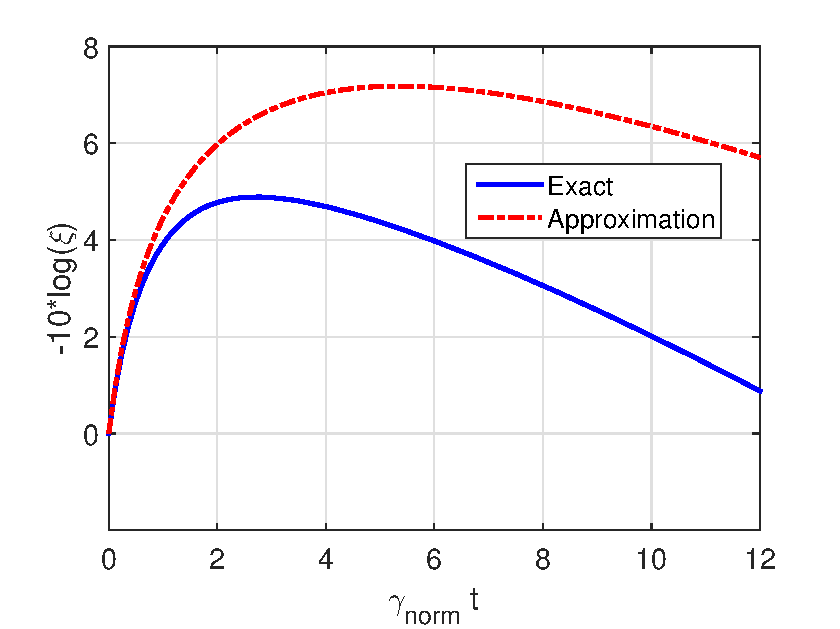
\includegraphics[scale=0.55]{./Figs/xi_magic33_yq}}
\end{minipage}
\begin{minipage}{.45\linewidth}
\centering
\subfloat[]{\label{fig:xi_magic44_yq}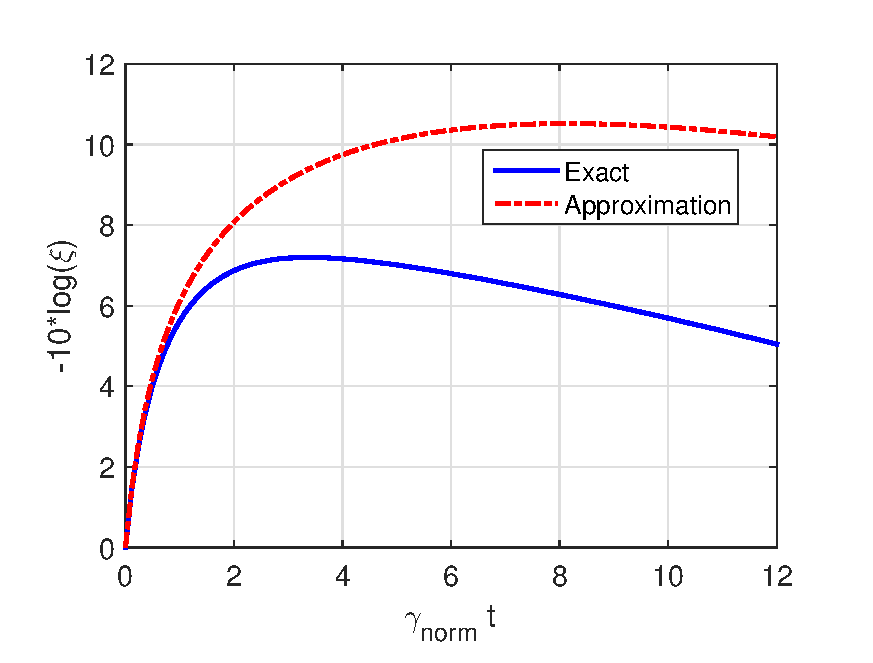
\includegraphics[scale=0.55]{./Figs/xi_magic44_yq}}
\end{minipage}
\par\medskip
\begin{minipage}{.45\linewidth}
\centering
\subfloat[]{\label{fig:xi_magic33_zq}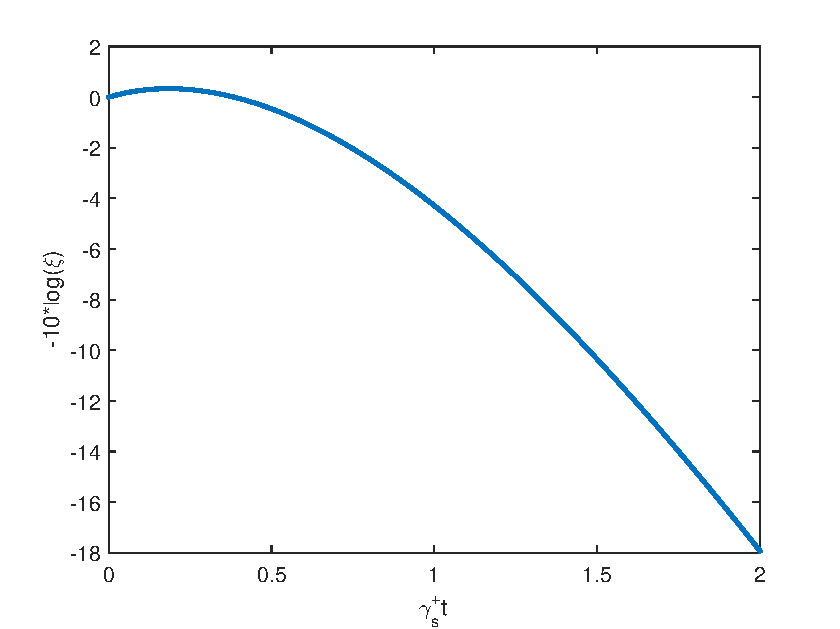
\includegraphics[scale=0.55]{./Figs/xi_magic33_zq}}
\end{minipage}
\begin{minipage}{.45\linewidth}
\centering
\subfloat[]{\label{fig:xi_magic44_zq}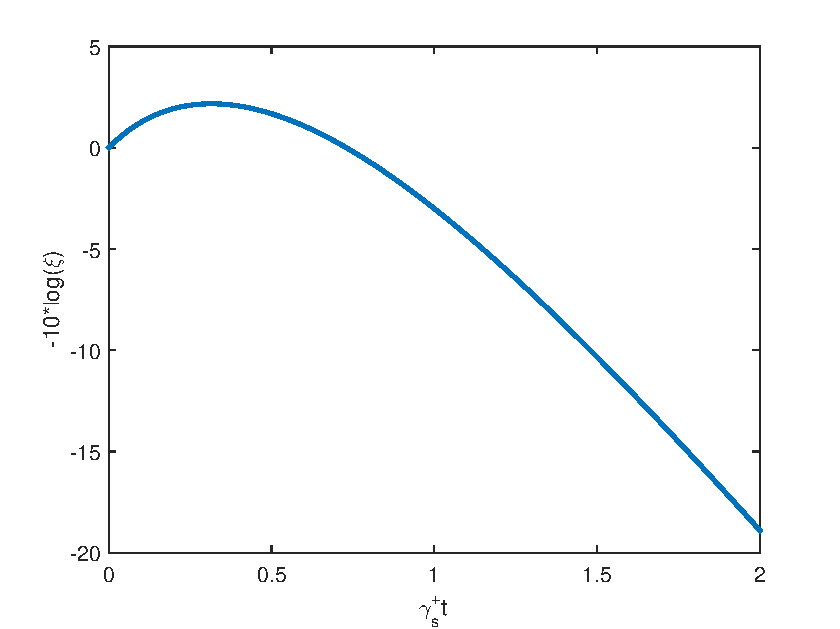
\includegraphics[scale=0.55]{./Figs/xi_magic44_zq}}
\end{minipage}
%\centering\makebox[\textwidth]{
%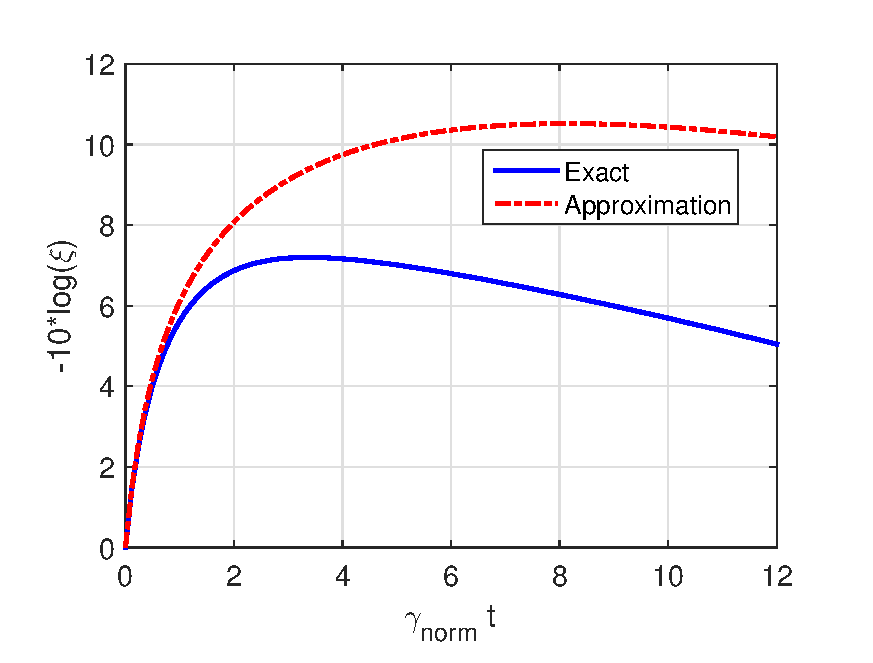
\includegraphics[width=0.65\textwidth]{./Figs/xi_magic44_yq}}
\caption{Spin squeezing evolution as a function of time with $ N_A=1000 $ atoms trapped at $ r'\!_\perp =1.5a $ along the $ H/x $-axis of the nanofiber. Subfigs.~\protect\subref{fig:xi_magic33_yq} and~\protect\subref{fig:xi_magic33_zq} use the magic frequencies close to the $ F=3\leftrightarrow F'=3 $ transition frequency $ \omega_{33'} $. Subfigs.~\protect\subref{fig:xi_magic44_yq} and~\protect\subref{fig:xi_magic44_zq} used the magic frequencies close to $ \omega_{44'} $. The magic frequencies and spin squeezing parameters are different for different choices of quantization axis. Subfigs.~\protect\subref{fig:xi_magic33_yq} and~\protect\subref{fig:xi_magic44_yq} define $ \phi $-axis as the quantization axis. In contrast, subfigs.~\protect\subref{fig:xi_magic33_zq} and~\protect\subref{fig:xi_magic44_zq} use $ z $-axis as the quantization axis. As can be seen, when the quantization axis close to the local field direction, the spin squeezing parameter can reach to a higher value. Other parameters used: $ \Omega/2\pi=52 $ MHz (does not matter). }\label{fig:xi_magic}
\end{figure}

...

\newpage

\subsubsection{The microscopic perspective analysis of continuous measurement and spin squeezing}

The measurement operator after the probe light interacting with the ensemble of atoms can be given by
\begin{align}
\hat{\mathcal{M}} &= \sum_i^{N_A} \int_0^T \mathrm{d}t' \hat{X}_{\bar{D}}^{\rm out} (z_D,t'-(z_{D}-z_i')/v_p),\label{eq:Mxout}
\end{align}
where $ T $ and $ Z_D $ are the integration time and position of the detector, $ z_i' $ is the $ z $-coordinate of the $ i $-th atom. 
 

For each atom, using the effective Hamiltonian that causes the birefringence effect, 
\begin{align}
\hat{H}_{\rm eff} &= \hbar \chi_{\rm eff} \sqrt{\frac{\dot{N}_L}{2}} \hat{F}_z \hat{P}_{\bar{D}}
\end{align}
one can find the equation of motion for the quadrature operator $ \hat{X}_{\bar{D}} $ to be
\begin{align}
\dt{\hat{X}_{\bar{D}}(z,t)} &= -\frac{i}{\hbar} \left[ \hat{H}_{\rm eff},\hat{X}_{\bar{D}} \right] \\
\Leftrightarrow \pp{\hat{X}_{\bar{D}}(z,t)}{t}+v_g\pp{\hat{X}_{\bar{D}}(z,t)}{z} &=  \chi_{\rm eff} \sqrt{\frac{\dot{N}_L}{2}} \hat{F}_z.
\end{align}
A formal solution can be given by
\begin{align}
\hat{X}_{\bar{D}} (z,t) &= \hat{X}_{\bar{D}}(0,t-z/v_p) + \sqrt{\frac{\kappa}{2}}\hat{F}_z(t-(z-z'_i)/v_p)\Theta(z-z'_i),
\end{align} 
where the measurement strength per atom is defined as $ \kappa = \chi_{\rm eff}^2 \dot{N}_L $. 

Using the result above, Equ.~\ref{eq:Mxout} gives
\begin{align}
\hat{\mathcal{M}} &= N_A\int_0^T\mathrm{d}t \hat{X}_{\bar{D}}(0,t-z_D/v_p) + N_AT\sqrt{\frac{\kappa}{2}}\hat{F}_z.
\end{align}
We have used the fact that all atoms around a nanofiber are interacting with the probe light in the same manner, and we have assumed the transition time of the light passing through the ensemble of atoms is much shorter than the atomic dynamics and the sampling time of the detector. 

...

Using the results above, one can write the stochastic master equation for the continuous measurement with the probe light discussed in this section...


\subsection{Sensitivity of the birefringence measurement using the clock states}
\textcolor{red}{To answer the question in this section: How to relate this to the critical shot noise limit--Equ.~\eqref{eq:shotnoise}?}  

For the birefringence measurement of the clock states discussed above, the fluctuation of the $ S_3 $ measurement is a combination effect of the shot noise fluctuation of the photon detector and the projection noise as the signal to determine the collective spin state:
\begin{align}
\Delta M^2 &= \Delta P^2_{SN} + \Delta P^2_S .
\end{align}
As have been discussed in Section~\ref{sec:birefringenceresolution}, the smallest detectable spin polarization is determined by the shot noise limit condition that 
\begin{align}
\Delta P_S = \Delta P_{SN},
\end{align}
where the standard variance of the signal can be estimated by
\begin{align}
\Delta P_S=P_0 \sin(\varphi_{_N}) \approx P_0 \varphi_{_N}
\end{align}
and the shot noise variance is determined by
\begin{align}
\Delta P_{SN} = \sqrt{\frac{P_0 \hbar \omega_0 }{2\eta \tau_{pd}}}.
\end{align}
We estimate the phase difference as
\begin{align}
\varphi_{_N} &= N_A \chi_{e\!f\!f}=N_A [(\chi_{H,\uparrow}-\chi_{H,\downarrow})-(\chi_{V,\uparrow}-\chi_{V,\downarrow})]\\
&= 2N_AC_{j'}^{(0)}(\Gamma_{H}^{1D}-\Gamma_V^{1D})\frac{1}{\Delta}=\frac{C_{j'}^{(0)}\sigma_0\Gamma_{vac}}{2}(\frac{1}{A^H_{e\!f\!f}}-\frac{1}{A^V_{e\!f\!f}})\frac{1}{\Delta}\\
&=N_AC_{j'}^{(0)}n_g\sigma_0\frac{\Gamma_{vac}}{2\Delta}\left[| \mathbf{u}_H(r'_{\!\perp})|^2- | \mathbf{u}_V(r'_{\!\perp})|^2 \right],
\end{align}
where $\frac{1}{\Delta}=\frac{1}{2}\sum_{f'}(\frac{1}{\Delta_{f',4}}-\frac{1}{\Delta_{f',3}})\approx \frac{1}{\Delta_{f',4}}$.

Now, we consider the critical case: $\eta =100\%$ and $\tau_{pd} = \frac{1}{\gamma_s}$, where the photon scattering rate
\begin{align*}
\gamma_s &= \sigma(\Delta) \frac{I(\br')}{\hbar \omega_0} \\
\sigma(\Delta) &=\frac{\sigma_0}{1+\frac{4\Delta^2}{\Gamma^2_{vac}}}\approx \sigma_0 \frac{\Gamma_{vac}^2}{4\Delta^2} \quad \text{(far detuning.)}
\end{align*}
We can rewrite 
\begin{align}
\Delta P_{SN} &=P_0\sqrt{\frac{ \sigma_0 }{2A_{in}}}\frac{\Gamma_{vac}}{2\Delta},\\
\Delta P_S &= N_A C_{j'}^{(0)}P_0 \frac{\sigma_0}{A_{e\!f\!f}}\frac{\Gamma_{vac}}{2\Delta}, 
\end{align}
with the effective mode areas
\begin{align}
A_{in } &= \frac{P_0}{I(\br')}=\frac{2}{| \mathbf{u}_H(r'_{\!\perp})|^2+ | \mathbf{u}_V(r'_{\!\perp})|^2},\\
A_{e\!f\!f} &= \frac{1}{n_g\left[ | \mathbf{u}_H(r'_{\!\perp})|^2- | \mathbf{u}_V(r'_{\!\perp})|^2\right]}.
\end{align}
Therefore, the $ \Delta P_S = \Delta P_{SN}$ condition gives the resolution of the birefringence measurement in terms of the minimum atom number as
\begin{align}
N^{min}_A &= \frac{1}{C_{j'}^{(0)}}\sqrt{\frac{A_{e\!f\!f}^2}{A_{in}\sigma_0}}.
\end{align}



\textcolor{red}{Work in progress...} 



\appendix
\chapter{Maxwell's Equations of an waveguide}
This chapter will dedicate to some fundamental theory of Maxwell's equations. More detailed 
discussions can be found in Ref.\cite{Snyder1983}. Some detailed solution of Maxwell's equation 
applied to  cylindrical structures can be found in Ref.\cite{Wait}. 

For nonmagnetic materials which normally constitute an optical waveguide with $ \mu=\mu_0 $, the 
spatial dependence of the electrical field $ \boldsymbol{\mathcal{E}}(\br) $ and the magnetic field $ 
\boldsymbol{\mathcal{H}}(\br) $ of an optical waveguide is determined by Maxwell's equations:
\begin{align}
\nabla\times \boldsymbol{\mathcal{E}} &= i(\mu_0/\varepsilon_0)^{1/2} k \boldsymbol{\mathcal{H}}, & 
\nabla\times \boldsymbol{\mathcal{H}} &= \boldsymbol{\mathcal{J}}-i(\varepsilon_0/\mu_0)^{1/2}kn^2 
\boldsymbol{\mathcal{E}}, \label{EHtimesMKS}\\
\nabla\cdot (n^2 \boldsymbol{\mathcal{E}}) &= \rho/\varepsilon_0, & \nabla\cdot 
\boldsymbol{\mathcal{H}} &=0, \label{EHdotsMKS}
\end{align}
where $ \boldsymbol{\mathcal{J}} $ and $ \rho $ are the current density and charge density, $ 
\varepsilon=n^2 \varepsilon_0 $ is the dielectric constant of the waveguide as a function of space, and $ 
k=2\pi/\lambda=\omega/c $.  We usually assume an implicit time dependence $ \exp(-i\omega t) $ in the 
full field vectors. These equations are written in MKS units, which are used by default. 

Sometimes, to avoid the dielectric constant $ \varepsilon_0 $ and magnetic permeability $ \mu_0 $ of 
free space, we can rewrite the Maxwell's equations in Gaussian units, which yield
\begin{align}
\nabla \times \boldsymbol{\mathcal{E}} &= -\frac{1}{c} \pt{\boldsymbol{\mathcal{B}}}=i 
k\boldsymbol{\mathcal{B}}, & \nabla \times 
\boldsymbol{\mathcal{H}} &= \frac{4\pi}{c} \boldsymbol{\mathcal{J}} + 
\frac{1}{c}\pt{\boldsymbol{\mathcal{D}}}= \frac{4\pi}{c}\boldsymbol{\mathcal{J}} 
-ik\boldsymbol{\mathcal{D}},\\
\nabla \cdot \boldsymbol{\mathcal{D}} &= 4\pi \rho, & \nabla \cdot \boldsymbol{\mathcal{B}} &=0,
\end{align}
where $ \boldsymbol{\mathcal{D}} = \varepsilon \boldsymbol{\mathcal{E}} $ and $ 
\boldsymbol{\mathcal{H}}= \boldsymbol{\mathcal{B}} $. 

\section{Fields of translationally invariant waveguides}
We define the axis of the waveguide is along $ z $-direction, and the refractive index profile of the 
waveguide is independent of $ z $, i.e. $ n=n(\br\!_\perp) $, which means the waveguide is 
translationally invariant. The fields of the waveguide can then be rewritten in a separable form
\begin{align}
\bmc{E}(\br) &= \bmc{E}(\br\!_\perp)\exp(i\beta z), & \bmc{H}(\br) &= \bmc{H}(\br\!_\perp)\exp(i\beta 
z),
\end{align}
where $ \beta $ is the propagation constant, and $ \br\!_\perp $ is the position vector in the transverse 
plane perpendicular to the $ z $-axis. We can further decompose these fields into longitudinal and 
transverse components, parallel and orthogonal to the waveguide axis, respectively, and denoted by 
subscripts $ z $ and $ \perp $. That is
\begin{align}\label{EHtranslong}
\bmc{E}(\br) &= \left( \bmc{E}\!_\perp + \mathcal{E}_z \hat{e}_z \right)\exp(i\beta z), & \bmc{H}(\br) &= 
\left( \bmc{H}\!_\perp + \mathcal{H}_z \hat{e}_z\right) \exp(i\beta z)
\end{align}

Notice that, the sign of $ \beta $ indicates the propagating direction of the fields. By definition, positive 
and negative $ \beta $'s correspond to forward- and backward-propagating fields. 

\section{Relationships between field components}\label{MWE:components}
By substituting Equ.~\ref{EHtranslong} into the source-free Maxwell equations 
(Equs.~\ref{EHtimesMKS} and~\ref{EHdotsMKS} with $ \bmc{J}=0,\, \rho=0 $), and comparing 
longitudinal and transverse components, we obtain the relationships between fields components as 
below
\begin{subequations}
\label{EHtz0}
\begin{align}
\bmc{E}\!_\perp &= -\left(\frac{\mu_0}{\varepsilon_0} \right)^{1/2} \frac{1}{kn^2} \hat{e}_z \times 
\left(\beta \bmc{H}\!_\perp + i\nabla\!_\perp \mathcal{H}_z \right),\\
\bmc{H}\!_\perp &= \left(\frac{\varepsilon_0}{\mu_0} \right)^{1/2} \frac{1}{k} \hat{e}_z \times \left(\beta 
\bmc{E}\!_\perp +i\nabla\!_\perp \mathcal{E}_z \right),\\
\mathcal{E}_z &= i\left(\frac{\mu_0}{\varepsilon_0} \right)^{1/2} \frac{1}{kn^2} \hat{e}_z \cdot 
\nabla\!_\perp \times \bmc{H}\!_\perp = \frac{i}{\beta} \left( \nabla\!_\perp \cdot \bmc{E}\!_\perp + 
(\bmc{E}\!_\perp \cdot \nabla\!_\perp) \ln n^2 \right),\\
\mathcal{H}_z &= -i \left(\frac{\varepsilon_0}{\mu_0} \right)^{1/2} \frac{1}{k}\hat{e}_z \cdot 
\nabla\!_\perp \times \bmc{E}\!_\perp = \frac{i}{\beta} \nabla\!_\perp \cdot \bmc{H}\!_\perp. 
\end{align}
\end{subequations}

Now we consider the waveguide of cylindrical fiber case. Due to symmetry, we tend to use the 
cylindrical coordinate system, which gives 
\begin{align}
\nabla\!_\perp = \hat{r}\!_\perp \pp{}{r\!_\perp} + \hat{\phi} \frac{1}{r\!_\perp} \pp{}{\phi}.
\end{align}
Therefore, Equ.~\ref{EHtz0} implies that the transverse components can be expressed in terms of the 
longitudinal components by
\begin{subequations}
\begin{align}
\mathcal{E}_{r\!_\perp} &= \frac{i}{h^2} \left[ \beta \pp{\mathcal{E}_z }{r\!_\perp} + 
\left(\frac{\mu_0}{\varepsilon_0} \right)^{1/2}  \frac{k}{r\!_\perp} 
\pp{\mathcal{H}_z}{\phi} \right], \\
\mathcal{E}_\phi &= \frac{i}{h^2} \left[\frac{\beta}{r\!_\perp} 
\pp{\mathcal{E}_z}{\phi} -\left(\frac{\mu_0}{\varepsilon_0} \right) ^{1/2} k 
\pp{\mathcal{H}_z}{r\!_\perp} 
\right],\\
\mathcal{H}_{r\!_\perp} &= \frac{i}{h^2} \left[ \beta \pp{\mathcal{H}_z}{r\!_\perp} 
-\left(\frac{\varepsilon_0}{\mu_0} \right)^{1/2} \frac{kn^2}{r\!_\perp}\pp{\mathcal{E}_z}{\phi} \right],\\
\mathcal{H}_\phi &= \frac{i}{h^2} \left[ \frac{\beta}{r\!_\perp} \pp{\mathcal{H}_z}{\phi} + 
\left(\frac{\varepsilon_0}{\mu_0} \right)^{1/2} kn^2 \pp{\mathcal{E}_z}{r\!_\perp} \right],
\end{align}
\end{subequations}
with $ h^2= k^2n^2-\beta^2=k^2 \varepsilon_f -\beta^2  $ and $ n=n(\br\!_\perp) $. 

Correspondingly, the component relationships in Gauss units are
\begin{subequations}\label{EHzgauss}
\begin{align}
\mathcal{E}_{r\!_\perp} &= \frac{i}{h^2} \left[ \beta \pp{\mathcal{E}_z }{r\!_\perp} + 
  \frac{k}{r\!_\perp} 
\pp{\mathcal{H}_z}{\phi} \right]= \frac{i\beta}{h^2} \pp{\mathcal{E}_z }{r\!_\perp} - 
  \frac{km}{r\!_\perp h^2} {\mathcal{H}_z}, \\
\mathcal{E}_\phi &= \frac{i}{h^2} \left[\frac{\beta}{r\!_\perp} 
\pp{\mathcal{E}_z}{\phi} - k 
\pp{\mathcal{H}_z}{r\!_\perp} 
\right] = -\frac{\beta m}{r\!_\perp h^2} 
{\mathcal{E}_z} - \frac{ik}{h^2} 
\pp{\mathcal{H}_z}{r\!_\perp},\\
\mathcal{H}_{r\!_\perp} &= \frac{i}{h^2} \left[ \beta \pp{\mathcal{H}_z}{r\!_\perp} 
- \frac{kn^2}{r\!_\perp}\pp{\mathcal{E}_z}{\phi} \right]= \frac{i\beta}{h^2} \pp{\mathcal{H}_z}{r\!_\perp} 
+ \frac{kn^2m}{r\!_\perp h^2} {\mathcal{E}_z},\\
\mathcal{H}_\phi &= \frac{i}{h^2} \left[ \frac{\beta}{r\!_\perp} \pp{\mathcal{H}_z}{\phi} + 
 kn^2 \pp{\mathcal{E}_z}{r\!_\perp} \right] = -\frac{\beta m}{r\!_\perp h^2} {\mathcal{H}_z} + 
  \frac{ikn^2}{h^2} \pp{\mathcal{E}_z}{r\!_\perp}.
\end{align}
\end{subequations}


\textcolor{red}{Vector and Scalar operators...}

\textcolor{red}{Vector wave equations...}

In Gauss units, we have 
\begin{align}
-\nabla\times (\nabla\times \mathbf{E})-\frac{\varepsilon}{c^2} \spt{\mathbf{E}} = 
-\frac{4\pi}{c}\mathbf{J}.
\end{align}
We can further simplify the equation above by using 
\begin{align}
\nabla\times (\nabla\times \bmc{E}) &= -\nabla(\nabla\cdot \bmc{E})+ \nabla^2\bmc{E}\\
-\frac{\varepsilon}{c^2} \spt{\mathbf{E}} &= \frac{\varepsilon\omega^2}{c^2}\spt{\bmc{E}}.
\end{align}

\chapter{Some Basic Properties of Bessel Functions}
Below, we collect some basic properties of Bessel functions without proving. Detailed properties of Bessel functions can be found in some books (see, for example, Ref.~\cite{Watson1995}).

Bessel's differential equation Bessel functions:
\begin{align}
x^2\sdd{R(x)}{x}+x\dd{R(x)}{x}+(x^2-m^2)R(x)=0,
\end{align}
where $R(x)$ is a Bessel function with index $m$. 

Recurrence relations for the first kind of Bessel functions:
\begin{align}
J_m(x)=\frac{m+1}{x}J_{m+1}(x)+\dd{J_{m+1}(x)}{x}=\frac{m-1}{x}J_{m-1}-\dd{J_{m-1}(x)}{x}.
\end{align}

Derivatives of Bessel functions:
\begin{align}
J_m^\prime(x)&=\frac{1}{2}(J_{m-1}(x)-J_{m+1}(x))\\
{H^{(1)}_m}^\prime (x) &=\frac{1}{2}({H^{(1)}_{m-1}}^\prime (x)-{H^{(1)}_{m+1}}^\prime(x))
\end{align}

\chapter{Cylindrical function decomposition of a tilted incident plane wave}\label{Ch:PlanewaveDecomposition}
As an example of applying the mode decomposition technique we used above to find the projected bounded and unbounded modes under cylindrical boundary conditions, below, we demonstrate a simple case on decomposing a tilted incident plane wave into corresponding cylindrical modes. The solution might be useful to give us some insights on solving the corresponding nanofiber problem when an external field presents, which is the case for some cooling and state preparation protocols demonstrated in experiments~\cite{Meng2017ground,Ostfeldt2017Dipole}. 

The key to solve this kind of problems is to decompose all field functions into cylindrical functions. The bare nanofiber modes have already been decomposed into cylindrical functions in the last section; therefore, here, we only need to decompose the incident field as cylindrical functions. 

We assume the incident plane wave is given by
\begin{equation}
\mathbf{E}(\br,t)=\re\left[\mathbf{U}(\br,t) \right]=\mathbf{E}_0 \cos (\mathbf{k}\cdot\mathbf{r}-\omega t + \phi_0),
\end{equation}
where the forward propagating wave can be given by
\begin{align}
\mathbf{U}(\br,t) &= \mathbf{U}_0e^{i(\mathbf{k}\cdot\mathbf{r}-\omega t + \phi_0)}\\
&= \mathbf{U}_0e^{i\mathbf{k}\cdot\mathbf{r}}e^{i(\phi_0-\omega t )}.
\end{align}
with the initial phase, $\phi_0$, and the vector amplitude of $\mathbf{U}_0$. We can ignore the phase offset, and separate the spatial and temporal parts for the forward-propagating field. We want to expand the plane wave function into cylindrical functions, and thus we can apply the technique we used in the last appendix to solve the boundary condition problem and decompose the bound and radiation modes. The only term that needs to be expanded is the $ e^{i\mathbf{k}\cdot\mathbf{r}} $ factor. 

We define $ \mathbf{k}\cdot\mathbf{r}=(k\!_{\perp}\mathbf{e}\!_{k\!_\perp}+k_z\mathbf{e}_{z}) \cdot(r\!_{\perp}\mathbf{e}\!_{r\!_\perp}+z\mathbf{e}_{z}) = k\!_{\perp}r\!_{\perp}\cos(\phi_{k}-\phi_{r})+k_{z}{z}= k\!_\perp r\!_\perp \cos \Delta\phi +k_{z}{z}$, where $ \Delta\phi=\phi_{k}-\phi_{r} \in [0,2\pi)$ is the angle between $ \mathbf{e}_{k\!_\perp} $ and $ \mathbf{e}_{r\!_\perp} $. Thus
\begin{align}
e^{i\mathbf{k}\cdot \mathbf{r}}=e^{ik\!_\perp r\!_\perp\cos\Delta\phi}e^{ik_{z}{z}}
\end{align}
is a periodic function of $ \Delta\phi $ and hence can be expanded into a Fourier series given below. 
\begin{align}
e^{i\mathbf{k}\cdot \mathbf{r}} &= \sum_{m=-\infty}^{\infty}c_{m}(k\!_\perp r\!_\perp)e^{im\Delta\phi}e^{ik_{z}{z}},
\end{align}
where the coefficients $ c_{m}(k\!_\perp r\!_\perp) $ is associated with Bessel's first integral\index{Bessel function!Bessel's first integral}~\footnote{see Jackson's E\&M of Ref.~\cite{Jackson1975}, on page 140.}
\begin{align}
c_{m}(k\!_\perp r\!_\perp)&= \frac{1}{2\pi} \int_0^{2\pi} e^{ik\!_\perp r\!_\perp\cos \Delta\phi}e^{-im\Delta\phi}\mathrm{d}\Delta\phi\\
&=i^mJ_m(k\!_\perp r\!_\perp).
\end{align}
Therefore, we have
\begin{align}
e^{i\mathbf{k}\cdot \mathbf{r}} &=\sum_{m=-\infty}^{\infty}i^me^{im\Delta\phi}e^{ik_{z}{z}}J_m(k\!_\perp r\!_\perp).
\end{align}

Notice that the first kind of Bessel's function\index{Bessel function!Bessel function of the first kind} usually represent standing radial waves, while Hankel functions\index{Hankel function} usually describe traveling waves. Using the relationships that $ J_{m}(k\!_\perp r\!_\perp)=H_{m}^{(1)}(k\!_\perp r\!_\perp)+H_{m}^{(2)}(k\!_\perp r\!_\perp) $, we can re-express the plane wave in terms of incoming (at negative r) and outgoing (at positive r) as below.
\begin{align}
e^{i\mathbf{k}\cdot \mathbf{r}} &=\sum_{m=-\infty}^{\infty}i^me^{im\Delta\phi}e^{ik_{z}{z}} H_{m}^{(1)}(k\!_\perp r\!_\perp)+\sum_{m=-\infty}^{\infty}i^me^{im\Delta\phi}e^{ik_{z}{z}} H_{m}^{(2)}(k\!_\perp r\!_\perp).
\end{align}

This result shows that only when $ k_z=\beta $ can the tilted plane wave contributes to nanofiber modes be with wavenumber $ \beta $, since both $ k_z $ and $ \beta $ have consistent physics meaning. Therefore, when a plane wave comes perpendicular to the fiber axis, the wave can rarely couple to the fiber's guided modes, which is good for minimizing the influence of the incident external field directly mixed into the detected signal at the end of the fiber. 

%\chapter{Project dipole radiation onto nanofiber modes: far field approximation (a rough model)}\label{ch:FreeDipoleProjection}
As a trial, we only add one atom in the nanofiber-trapped-atoms system. 
Considering the detector is far away from the atom compared to the distance between the atom and the nanofiber, the paraxial approximation\index{paraxial approximation} holds for our case where our measurement on the optical field is applied after a distant transmission through the fiber. \textcolor{red}{We also assume that the emission from the atom propagates in free space by vanishing the boundary condition defined by the nanofiber, so that we can use the conclusion of the Green function for free space. }
The scattered optical field can be written as 
\begin{align}
\boldsymbol{\mathcal{E}}^s(\br) &=-k_0^2\left(\boldsymbol{\alpha}\cdot \boldsymbol{\mathcal{E}}^g(\br')\right)_\perp \frac{e^{ik_0 \left| \br-\br' \right| }}{\left| \br-\br'\right| }\\
&=-k_0^2\left[ \boldsymbol{\alpha}\!\cdot\! \boldsymbol{\mathcal{E}}^g(\br') - \left(\hat{\mathrm{r}}\! \cdot\! \boldsymbol{\alpha}\!\cdot\! \boldsymbol{\mathcal{E}}^g(\br') \right) \hat{\mathrm{r}}\right] \frac{e^{ik_0 \left| \br-\br' \right| }}{\left| \br-\br'\right| }\\
&\approx -k_0^2\left[ \boldsymbol{\alpha}\!\cdot\! \boldsymbol{\mathcal{E}}^g(\br') - \left(\hat{\mathrm{e}}_z\! \cdot\! \boldsymbol{\alpha}\!\cdot\! \boldsymbol{\mathcal{E}}^g(\br') \right) \hat{\mathrm{e}}_z\right] \frac{e^{ik_0 \left| \br-\br' \right| }}{\left| \br-\br'\right| }\\
&=-k_0^2 \left[\left(\hat{\mathrm{e}}_{r_\perp} \! \cdot \! \boldsymbol{\alpha} \! \cdot\! \boldsymbol{\mathcal{E}}^g(\br')\right)\hat{\mathrm{e}}_{r_\perp} + \left(\hat{\mathrm{e}}_\phi \! \cdot \! \boldsymbol{\alpha} \! \cdot \! \boldsymbol{\mathcal{E}}^g(\br') \right)\hat{\mathrm{e}}_\phi \right] 
\frac{e^{ik_0 \left| \br-\br' \right| }}{\left| \br-\br'\right| }\\
&\approx \frac{-k_0^2 e^{ik_0(z\!-\!z'\!)}}{z\!-\!z'}\left[\left(\hat{\mathrm{e}}_{r_\perp} \!\!\cdot\! \boldsymbol{\alpha}\!\cdot\! \boldsymbol{\mathcal{E}}^g(\br')\right)\hat{\mathrm{e}}_{r_\perp} \!\! +\! \left(\hat{\mathrm{e}}_\phi\!\cdot\! \boldsymbol{\alpha}\!\cdot\! \boldsymbol{\mathcal{E}}^g(\br') \right)\hat{\mathrm{e}}_\phi \right] \exp\!\! \left[ \frac{ik_0 \left| \mathrm{r}_\perp\! - \mathrm{r}_\perp'\right|}{2(z-z')}  \right],\label{Erscatt}
\end{align}
where $ \boldsymbol{\alpha} $ is the polarizability tensor only depending on the internal state of the atom; $ \left| \mathrm{r}_\perp - \mathrm{r}_\perp'\right|=\sqrt{r_\perp^2+{r_\perp'}^2 - 2 r_\perp r_\perp'\cos(\phi-\phi')} $ where $ (r_\perp',\phi',z') $ is the coordinate of the atom. 

As shown in Equ.~\ref{Erscatt}, the scattered field does not have a $ z $-component in the far field by using a free space Green function. 

We can decompose the guided mode into left- and right-handed circular fundamental modes using Equ.~\ref{Eilincyc}. For instance, if the incident light is $ x $-polarized (horizontally polarized) with the normalized field $ \boldsymbol{\mathcal{E}}^g (\br)=\boldsymbol{\mathcal{E}}_H (\br) $, and $ \mathbf{E}^g (\br,t) = \boldsymbol{\mathcal{E}}_H(\br)e^{-i\omega t} $ is a forward propagating light, we can use the relationship that
\begin{subequations}
\label{ErPMHV}
\begin{align}
\boldsymbol{\mathcal{E}}^+ &= \frac{1}{\sqrt{2}} \left(\boldsymbol{\mathcal{E}}_H+i\boldsymbol{\mathcal{E}}_V \right),\\
\boldsymbol{\mathcal{E}}^- &= \frac{1}{\sqrt{2}} \left( \boldsymbol{\mathcal{E}}_H-i\boldsymbol{\mathcal{E}}_V \right),
\end{align}
\end{subequations}
where $ \boldsymbol{\mathcal{E}}_V $ is the normalized mode with a $ y $-polarized (vertically polarized) incident light which is orthogonal to $ \boldsymbol{\mathcal{E}}_H $. Based on Equ.~\ref{ErPMHV}, we can solve for $ \boldsymbol{\mathcal{E}}_H $ to give
\begin{align}
\boldsymbol{\mathcal{E}}_H &= \frac{1}{\sqrt{2}} \left(\boldsymbol{\mathcal{E}}^+ + \boldsymbol{\mathcal{E}}^- \right),\\
\boldsymbol{\mathcal{E}}_V &= \frac{i}{\sqrt{2}} \left( \boldsymbol{\mathcal{E}}^- -\boldsymbol{\mathcal{E}}^+ \right). 
\end{align}
Therefore, the spatial dependent scattered electrical field can be given by
\begin{align}
\boldsymbol{\mathcal{E}}^s(\br) &\approx  \frac{-\!k_0^2 e^{ik_0(z\!-\!z'\!)}}{z\!-\!z'}\! \left[\left(\hat{\mathrm{e}}_{r_\perp} \!\!\cdot\! \boldsymbol{\alpha}\!\cdot\! \boldsymbol{\mathcal{E}}_H(\br')\right)\hat{\mathrm{e}}_{r_\perp} \!\!  +\! \left(\hat{\mathrm{e}}_\phi\!\cdot\! \boldsymbol{\alpha}\!\cdot\! \boldsymbol{\mathcal{E}}_H(\br') \right)\hat{\mathrm{e}}_\phi \right] \exp\!\! \left[ \frac{ik_0 \left| \mathrm{r}_\perp\!\! -\! \mathrm{r}_\perp'\right|}{2(z-z')}  \right]\\
&= - \frac{k_0^2 e^{ik_0(z\!-\!z'\!)}}{\sqrt{2}(z\!-\!z')} \left(\hat{\mathrm{e}}_{r_\perp} \!\!\cdot\! \boldsymbol{\alpha}\!\cdot\! \left(\boldsymbol{\mathcal{E}}^+ (\br') \!\! +\! \boldsymbol{\mathcal{E}}^- (\br') \right)\right)\hat{\mathrm{e}}_{r_\perp}  \exp\!\! \left[ \frac{ik_0 \left| \mathrm{r}_\perp\!\! -\! \mathrm{r}_\perp'\right|}{2(z-z')}  \right] \nonumber\\
&\qquad - \frac{k_0^2 e^{ik_0(z\!-\!z'\!)}}{\sqrt{2}(z\!-\!z')} \left(\hat{\mathrm{e}}_{\phi} \!\!\cdot\! \boldsymbol{\alpha}\!\cdot\! \left(\boldsymbol{\mathcal{E}}^+ (\br') \!\! +\! \boldsymbol{\mathcal{E}}^- (\br') \right)\right)\hat{\mathrm{e}}_{\phi}  \exp\!\! \left[ \frac{ik_0 \left| \mathrm{r}_\perp\!\! -\! \mathrm{r}_\perp'\right|}{2(z-z')}  \right]. \label{Ers0}
\end{align}
Using Equs.~\ref{Ertcrla} and~\ref{Ertcrga}, the $ \boldsymbol{\mathcal{E}}_H (\br')= \boldsymbol{\mathcal{E}}^+ (\br') \!\! +\! \boldsymbol{\mathcal{E}}^- (\br') $ is given by
\begin{subequations}
\label{EHrcrla}
\begin{align}
{\mathcal{E}_H}_{r_\perp} (\br') &= A\frac{\beta_{11}}{h_{11}}\nonumber\\
&\qquad \left[ (1\!-\!s_{11})J_0(h_{11}r'_\perp)\!-\! (1\!+\!s_{11})J_2(h_{11}r_\perp') \right]e^{if\beta_{11} z'}\cos{\phi'}\\
{\mathcal{E}_H}_\phi(\br') &=  iA \frac{\beta_{11}}{2h_{11}} \nonumber\\
&\qquad \left[ (1\!-\!s_{11})J_0(h_{11}r'_\perp)\! +\! (1\!+\!s_{11})J_2(h_{11}r'_\perp) \right] e^{if\beta_{11} z' }\sin(\phi')\\
{\mathcal{E}_H}_z(\br') &= i2A J_1(h_{11}r'_\perp) e^{if\beta_{11} z'}\cos(\phi')
\end{align}
\end{subequations}
for $ r'_\perp<a $, and by
\begin{subequations}
\label{EHrpcrga}
\begin{align}
{\mathcal{E}_H}_{r_\perp}(\br') &=A\frac{\beta_{11}}{h_{11}}\frac{J_1(h_{11}a)}{K_1(q_{11}a)}\nonumber\\ 
&\qquad \left[ (1\!-\!s_{11})K_0(q_{11}r'_\perp)\!+\!(1 \!+\! s_{11})K_2(q_{11}r'_\perp) \right]e^{if\beta_{11} z' }\cos(\phi')\\
{\mathcal{E}_H}_\phi(\br') &=  iA \frac{\beta_{11}}{h_{11}} \frac{J_1(h_{11}a)}{K_1(q_{11}a)}\nonumber\\ 
&\qquad \left[ (1\!-\!s_{11})K_0(q_{11}r'_\perp) \! -\! (1\!+\!s_{11})K_2(q_{11}r'_\perp) \right] e^{if\beta_{11} z'}\sin(\phi')\\
{\mathcal{E}_H}_z(\br') &= i2A \frac{J_1(h_{11}a)}{K_1(q_{11}a)} K_1(q_{11}r'_\perp) e^{if\beta_{11} z'}\cos(\phi')
\end{align}
\end{subequations}
for $ r'_\perp>a $. We define $ \mathbf{T}^{f}(\br')= \boldsymbol{\alpha}\!\cdot \boldsymbol{\mathcal{E}}_H (\br') = \boldsymbol{\alpha}\!\cdot\! \left(\boldsymbol{\mathcal{E}}^+ (\br') \!\! +\! \boldsymbol{\mathcal{E}}^- (\br') \right) $, which is a constant vector, and only the $ r_\perp $ and $ \phi $ components contribute to the scattered field in the far field. Now, Equ.~\ref{Ers0} can be rewritten as
\begin{align}
\boldsymbol{\mathcal{E}}^s(\br) &=- \frac{k_0^2 e^{ik_0(z\!-\!z'\!)}}{\sqrt{2}(z\!-\!z')} \exp\!\! \left[ \frac{ik_0 \left| \mathrm{r}_\perp\!\! -\! \mathrm{r}_\perp'\right|}{2(z-z')}  \right]\! \left[ T_{r_\perp}^f(\br') \hat{\mathrm{e}}_{r_\perp} \! + T^f_\phi (\br') \hat{\mathrm{e}}_{\phi} \right],
\end{align}
where $ T^f_{r_\perp}(\br') $ and $ T^f_\phi (\br') $ are the $ r_\perp $ and $ \phi $ components of $ \mathbf{T}^f(\br')$. 

The total electrical field can be written as 
\begin{align}
\boldsymbol{\mathcal{E}}(\br) &= \boldsymbol{\mathcal{E}}^g(\br) + \boldsymbol{\mathcal{E}}^s(\br)\\
&\approx  \frac{1}{\sqrt{2}} \left(\boldsymbol{\mathcal{E}}^+(\br)\!\! +\! \boldsymbol{\mathcal{E}}^-(\br) \right) \nonumber\\
&\qquad - \frac{k_0^2 e^{ik_0(z\!-\!z'\!)}}{\sqrt{2}(z\!-\!z')} \left(\hat{\mathrm{e}}_{r_\perp} \!\!\cdot\! \boldsymbol{\alpha}\!\cdot\! \left(\boldsymbol{\mathcal{E}}^+ (\br') \!\! +\! \boldsymbol{\mathcal{E}}^- (\br') \right)\right)\hat{\mathrm{e}}_{r_\perp}  \exp\!\! \left[ \frac{ik_0 \left| \mathrm{r}_\perp\!\! -\! \mathrm{r}_\perp'\right|}{2(z-z')}  \right] \nonumber\\
&\qquad - \frac{k_0^2 e^{ik_0(z\!-\!z'\!)}}{\sqrt{2}(z\!-\!z')} \left(\hat{\mathrm{e}}_{\phi} \!\!\cdot\! \boldsymbol{\alpha}\!\cdot\! \left(\boldsymbol{\mathcal{E}}^+ (\br') \! +\! \boldsymbol{\mathcal{E}}^- (\br') \right)\right)\hat{\mathrm{e}}_{\phi}  \exp\!\! \left[ \frac{ik_0 \left| \mathrm{r}_\perp\!\! -\! \mathrm{r}_\perp'\right|}{2(z-z')}  \right]\\
&= \frac{1}{\sqrt{2}} \boldsymbol{\mathcal{E}}_H(\br)  \!-\! \frac{k_0^2 e^{ik_0(z\!-\!z'\!)}}{\sqrt{2}(z\!-\!z')} \exp\!\! \left[ \frac{ik_0\! \left| \mathrm{r}_\perp\!\! -\! \mathrm{r}_\perp'\right|}{2(z-z')}  \right]\!\! \left[ T^f_{r_\perp}(\br') \hat{\mathrm{e}}_{r_\perp} \!\! +\! T^f_\phi (\br') \hat{\mathrm{e}}_{\phi} \right].
\end{align}
%where $ \eye $ is the unitary diagonal tensor. Now, we can see that the total optical field strongly depends on the bound field and the polarization of the atom.

To further discuss how backward and forward scattering contribute to the bound mode, we consider both the space- and time-dependent electrical field of the scattered contribution $ \mathbf{E}^s(\br,t) $, and project it to the normalized forwarded and backwarded bound modes.  In principle, we can decompose the scattered electrical field as 
\begin{align}
\mathbf{E}^s(\br,t) =\sum_\mu C^{(\mu)}(z) \mathbf{E}^{(\mu)} (\br,t),
\end{align}
with
\begin{align}
C^{(\mu)} (z) = \int_0^{2\pi}\mathrm{d}\phi \int_0^\infty {\mathbf{E}^{(\mu)}}^* (\br,t) \cdot \mathbf{E}^s(\br,t)r_\perp \mathrm{d}r_\perp.
\end{align}

For the Green function we used above, the coefficients in the far field can be calculated as
\begin{align}
C^{(\mu)} (z) &= - \frac{k_0^2 T^{f'}_{r_\perp}(\br') e^{ik_0(z\!-\!z'\!)}}{\sqrt{2}(z\!-\!z')}\int_0^{2\pi}\mathrm{d}\phi \int_0^\infty {\mathcal{E}^{(\mu)}_{r_\perp}}^* (\br) \exp\!\! \left[ \frac{ik_0 \left| \mathrm{r}_\perp\!\! -\! \mathrm{r}_\perp'\right|}{2(z-z')}  \right]\!  r_\perp \mathrm{d}r_\perp \nonumber\\
&\quad - \frac{k_0^2 T^{f'}_\phi(\br') e^{ik_0(z\!-\!z'\!)} }{\sqrt{2}(z\!-\!z')}\int_0^{2\pi}\mathrm{d}\phi \int_0^\infty {\mathcal{E}^{(\mu)}_\phi}^* (\br) \exp\!\! \left[ \frac{ik_0 \left| \mathrm{r}_\perp\!\! -\! \mathrm{r}_\perp'\right|}{2(z-z')}  \right]\!  r_\perp \mathrm{d}r_\perp \\
&=  - \frac{k_0^2 T^{f'}_{r_\perp}(\br') e^{ik_0(z\!-\!z'\!)}}{\sqrt{2}(z\!-\!z')}\int_0^{2\pi}\mathrm{d}\phi \int_0^a {\mathcal{E}^{(\mu)}_{r_\perp}}^* (\br) \exp\!\! \left[ \frac{ik_0 \left| \mathrm{r}_\perp\!\! -\! \mathrm{r}_\perp'\right|}{2(z-z')}  \right]\!  r_\perp \mathrm{d}r_\perp \nonumber\\
&\quad - \frac{k_0^2 T^{f'}_{r_\perp}(\br') e^{ik_0(z\!-\!z'\!)}}{\sqrt{2}(z\!-\!z')}\int_0^{2\pi}\mathrm{d}\phi \int_a^\infty {\mathcal{E}^{(\mu)}_{r_\perp}}^* (\br) \exp\!\! \left[ \frac{ik_0 \left| \mathrm{r}_\perp\!\! -\! \mathrm{r}_\perp'\right|}{2(z-z')}  \right]\!  r_\perp \mathrm{d}r_\perp \nonumber\\
&\quad - \frac{k_0^2 T^{f'}_\phi(\br') e^{ik_0(z\!-\!z'\!)}}{\sqrt{2}(z\!-\!z')}\int_0^{2\pi}\mathrm{d}\phi \int_0^a {\mathcal{E}^{(\mu)}_\phi}^* (\br) \exp\!\! \left[ \frac{ik_0 \left| \mathrm{r}_\perp\!\! -\! \mathrm{r}_\perp'\right|}{2(z-z')}  \right]\!  r_\perp \mathrm{d}r_\perp \nonumber\\
&\quad - \frac{k_0^2 T^{f'}_\phi(\br') e^{ik_0(z\!-\!z'\!)}}{\sqrt{2}(z\!-\!z')}\int_0^{2\pi}\mathrm{d}\phi \int_a^\infty {\mathcal{E}^{(\mu)}_\phi}^* (\br) \exp\!\! \left[ \frac{ik_0 \left| \mathrm{r}_\perp\!\! -\! \mathrm{r}_\perp'\right|}{2(z-z')}  \right]\!  r_\perp \mathrm{d}r_\perp \\
&= - \frac{k_0^2 T^{f'}_{r_\perp}(\br') e^{ik_0(z\!-\!z'\!)\!-\!if\beta_{11} z}}{\sqrt{2}(z\!-\!z')}  \!\!\! \int_0^{2\pi}\!\!\! \mathrm{d}\phi \!\!\! \int_0^a   \mathcal{E}^{(\mu)}_{r_\perp}(r_\perp) e^{-i p\phi} 
\exp\!\! \left[ \frac{ik_0 \left| \mathrm{r}_\perp\!\! -\! \mathrm{r}_\perp'\right|}{2(z-z')}  \right]\!  r_\perp \mathrm{d}r_\perp \nonumber\\
&\quad - \frac{k_0^2 T^{f'}_{r_\perp}(\br') e^{ik_0(z\!-\!z'\!)\!-\!if\beta_{11} z}}{\sqrt{2}(z\!-\!z')}  \!\!\! \int_0^{2\pi}\!\!\! \mathrm{d}\phi \!\!\! \int_a^\infty \!\!\! {\mathcal{E}^{(\mu)}_{r_\perp}} (r_\perp) e^{-i p\phi} \exp\!\! \left[ \frac{ik_0 \left| \mathrm{r}_\perp\!\! -\! \mathrm{r}_\perp'\right|}{2(z-z')}  \right]\!  r_\perp \mathrm{d}r_\perp \nonumber\\
&\quad - \frac{k_0^2 T^{f'}_\phi(\br') e^{ik_0(z\!-\!z'\!)\!-\!if\beta_{11} z}}{\sqrt{2}(z\!-\!z')} \!\!\! \int_0^{2\pi}\!\!\! \mathrm{d}\phi \!\!\! \int_0^a \!\!\! {\mathcal{E}^{(\mu)}_\phi} (r_\perp) e^{-i p\phi} \exp\!\! \left[ \frac{ik_0 \left| \mathrm{r}_\perp\!\! -\! \mathrm{r}_\perp'\right|}{2(z-z')}  \right]\!  r_\perp \mathrm{d}r_\perp \nonumber\\
&\quad - \frac{k_0^2 T^{f'}_\phi(\br') e^{ik_0(z\!-\!z'\!)\!-\!if\beta_{11} z}}{\sqrt{2}(z\!-\!z')}  \!\!\! \int_0^{2\pi}\!\!\!\mathrm{d}\phi\!\!\!  \int_a^\infty \!\!\! {\mathcal{E}^{(\mu)}_\phi} (r_\perp) e^{-i p\phi} \exp\!\! \left[ \frac{ik_0 \left| \mathrm{r}_\perp\!\! -\! \mathrm{r}_\perp'\right|}{2(z-z')}  \right]\!  r_\perp \mathrm{d}r_\perp \\
&=  - \frac{k_0^2 T^{f'}_{r_\perp}(\br') e^{ik_0(z\!-\!z'\!)\!-\!if\beta_{11} z}}{\sqrt{2}(z\!-\!z')} \!\! \int_0^{2\pi}\!\!\! \mathrm{d}\phi \!\! \int_0^a  \!\! \mathcal{E}^{(\mu)}_{r_\perp}(r_\perp)  
\exp\!\! \left[ \frac{ik_0 \left| \mathrm{r}_\perp\!\! -\! \mathrm{r}_\perp'\right|}{2(z-z')} \!-\! i p\phi  \right]\!  r_\perp \mathrm{d}r_\perp \nonumber\\
&\quad - \frac{k_0^2 T^{f'}_{r_\perp}(\br') e^{ik_0(z\!-\!z'\!)\!-\!if\beta_{11} z}}{\sqrt{2}(z\!-\!z')}  \!\!\! \int_0^{2\pi}\!\!\!\mathrm{d}\phi \!\!\! \int_a^\infty \!\!\! {\mathcal{E}^{(\mu)}_{r_\perp}} (r_\perp)  \exp\!\! \left[ \frac{ik_0 \left| \mathrm{r}_\perp\!\! -\! \mathrm{r}_\perp'\right|}{2(z-z')} \!-\! i p\phi \right]\!  r_\perp \mathrm{d}r_\perp \nonumber\\
&\quad - \frac{k_0^2 T^{f'}_\phi(\br') e^{ik_0(z\!-\!z'\!)\!-\!if\beta_{11} z}}{\sqrt{2}(z\!-\!z')} \!\!\! \int_0^{2\pi} \!\!\! \mathrm{d}\phi \!\!\! \int_0^a\!\!\! {\mathcal{E}^{(\mu)}_\phi} (r_\perp) \exp\!\! \left[ \frac{ik_0 \left| \mathrm{r}_\perp\!\! -\! \mathrm{r}_\perp'\right|}{2(z-z')} \!-\! i p\phi \right]\!  r_\perp \mathrm{d}r_\perp \nonumber\\
&\quad - \frac{k_0^2 T^{f'}_\phi(\br') e^{ik_0(z\!-\!z'\!)\!-\!if\beta_{11} z}}{\sqrt{2}(z\!-\!z')}  \!\!\! \int_0^{2\pi}\!\!\! \mathrm{d}\phi \!\!\! \int_a^\infty \!\!\! {\mathcal{E}^{(\mu)}_\phi} (r_\perp) \exp\!\! \left[ \frac{ik_0 \left| \mathrm{r}_\perp\!\! -\! \mathrm{r}_\perp'\right|}{2(z-z')} \!-\! i p\phi \right]\!  r_\perp \mathrm{d}r_\perp. \label{Cmu1}
\end{align}
Using the relationship that $ \left| \mathrm{r}_\perp - \mathrm{r}_\perp'\right|=\sqrt{r_\perp^2+{r_\perp'}\!\!^2 - 2 r_\perp r_\perp'\cos(\phi-\phi')} $, the integral over $ \phi $ can be separated as 
\begin{align}
C^{(\mu)}_0(r_\perp,z) &= \int_0^{2\pi} \!\!\! \mathrm{d}\phi  \exp\!\! \left[ \frac{ik_0 \left| \mathrm{r}_\perp\!\! -\! \mathrm{r}_\perp'\right|}{2(z-z')} \!-\! i p\phi \right]\\
&= \int_0^{2\pi} \!\!\! \mathrm{d}\phi  \exp\!\! \left[ \frac{ik_0 \sqrt{r_\perp^2+{r_\perp'}\!\!^2 - 2 r_\perp r_\perp'\cos(\phi-\phi')} }{2(z-z')} \!-\! i p\phi \right]\\
&= \int_0^{2\pi} \!\!\! \mathrm{d}\phi  \exp\!\! \left[ \frac{ik_0 \sqrt{r_\perp^2 \!+ {r_\perp'}\!\!^2}\sqrt{1 \!-\! \frac{2 r_\perp r_\perp'}{r_\perp^2 \!+ {r_\perp'}\!\!^2}\cos(\phi \!-\! \phi')} }{2(z-z')} \!-\! i p\phi \right].
\end{align}
Calculating this integration analytically is not trivial unless $ r_\perp=r_\perp' $ or $ \br_\perp $ parallel to $ \br_\perp' $. We can calculate the projection coefficients numerically instead. Equ.~\ref{Cmu1} can be rewritten as
\begin{align}
C^{(\mu)} (z) &= - \frac{k_0^2 e^{ik_0(z\!-\!z'\!)\!-\!if\beta_{11} z} }{\sqrt{2}(z\!-\!z')}\left[  T^{f'}_{r_\perp}(\br') \mathcal{C}_{r_\perp}^p (z) +  T^{f'}_\phi(\br') \mathcal{C}_{\phi}^p(z) \right]\\
&= T^{f'}_{r_\perp}(\br') \mathcal{S}_{r_\perp}^p (z) +  T^{f'}_\phi(\br') \mathcal{S}_{\phi}^p(z),
\end{align}
where $ \mathcal{C}_{r_\perp}^p(z) $ and $ \mathcal{C}_\phi^p(z) $ correspond to the integrals with $ \mathcal{E}^{(\mu)}_{r_\perp} $ and $ \mathcal{E}^{(\mu)}_{\phi} $, repectively; Correspondingly, $ \mathcal{S}_{r_\perp}^p(z)=\mathcal{A}(z)\mathcal{C}_{r_\perp}^p(z) $ and $ \mathcal{S}_{\phi}^p(z)=\mathcal{A}(z)\mathcal{C}_\phi^p(z) $, where the interference factor
\begin{align}
\mathcal{A}(z) &= - \frac{k_0^2  e^{ik_0(z\!-\!z'\!)\!-\!if\beta_{11} z}}{\sqrt{2}(z\!-\!z')}.
\end{align} 

We made $ \br'=(r'_\perp,\phi',z')=(2a,0,0) $ and $ \lambda_0=937.1 $ nm, and numerically calculated the projection coefficients for the forward propagating and counterclockwise polarized fundamental mode. The results are shown in Figs~\ref{Cz} and~\ref{ACSz}. Notice that, due to numerical inaccuracy, there are some divergent integration noises for $ z<5 $ cm. As we can see from the figures, $ \mathcal{A}(z) $ is a result of the interference of the point-scattered light and the bound mode, which decays as a function of $ \frac{1}{z-z'} $ with a periodical phase change. The phase change should have a period of $ 2\pi/(k_0-\beta_{11})\sim \lambda_0 $, where $ \beta_{11} $ is about one tenth of $ k_0 $. Due to limited computing resolution, the plots in Fig.~\ref{ACSz} does not reflect the correct phase changing period. $ \mathcal{C}^{(\mu)}(z) $ reflects how the scattered light synchronizes and better coupled with the bound mode as $ z $ increases. Combining these factors, the total projection factor $ \mathcal{S}^{(\mu)}(z) $ decays dramatically when $ z $ is small as the $ \frac{1}{z-z'} $ propagating decay dominates, and then increases with a periodical-like oscillation as the scattered light is close to a plane wave and can be well coupled and interfered with the bound mode. The beating frequency increases as the light propagates until it can be well coupled with the bound mode. Both $ r_\perp $ and $ \phi $ components of the projection coefficients have some difference as $ z $ is large. 

\textcolor{red}{Here are some phenomena needed to further explain}: the different periods of changes for $ r_\perp< a $ and $ r_\perp>a $ cases; interference periods and beating periods are not as simple as normal interference model predicted (see Fig.~\ref{../media/Figs/InterferencePeriods})--this is because we used a rough resolution in $ z $-direction to save computing time; the different behaviors of the two transverse components of the projection coefficients...

\textcolor{red}{Technical problem: numerical integration does not work well for high oscillating functions. We need to artificially set up a very fine integrating $ x $-axis to make it work properly. To fully solve this problem, we may need to consider better integration method, such as chebfun developed by Oxford (\url{http://www2.maths.ox.ac.uk/chebfun/}) which, I believe, is powerful to solve problems including definite integration, ordinary differential equations, contour integrals and roots finding. }

%\scalefig{Figs/Cr1}{0.5}{$ \mathcal{C}_{r_\perp} $ for $ r_\perp < a $ as a function of $ z $.}
\begin{figure}[H] 
\begin{minipage}{.5\linewidth}
\centering
\subfloat[$ \mathcal{C}_{r_\perp}(z) $ for $ r_\perp < a $]{\label{Cza}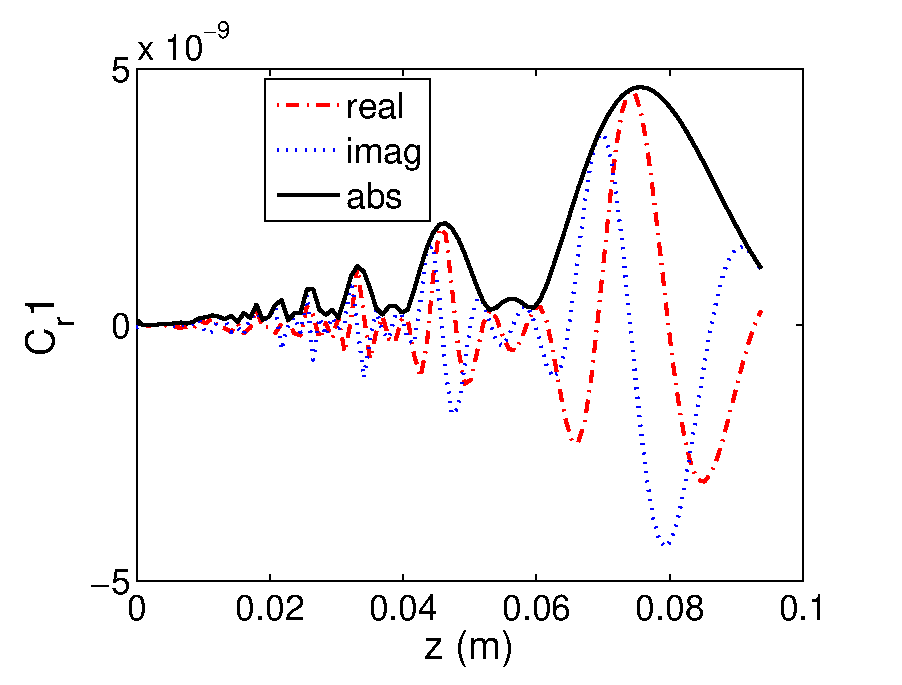
\includegraphics[scale=.44]{../media/Figs/Cr1}}
\end{minipage}%
\begin{minipage}{.5\linewidth}
\centering
\subfloat[$ \mathcal{C}_{r_\perp}(z) $ for $ r_\perp > a $]{\label{Czb}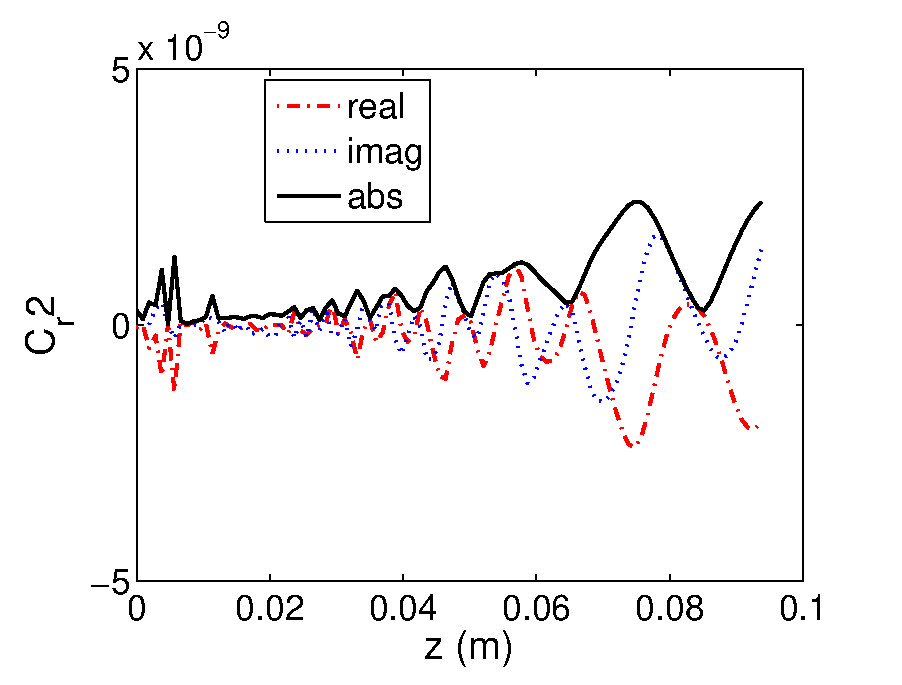
\includegraphics[scale=.44]{../media/Figs/Cr2}}
\end{minipage}
\par\medskip
\begin{minipage}{.5\linewidth}
\centering
\subfloat[$ \mathcal{C}_\phi(z) $ for $ r_\perp < a $]{\label{Czc}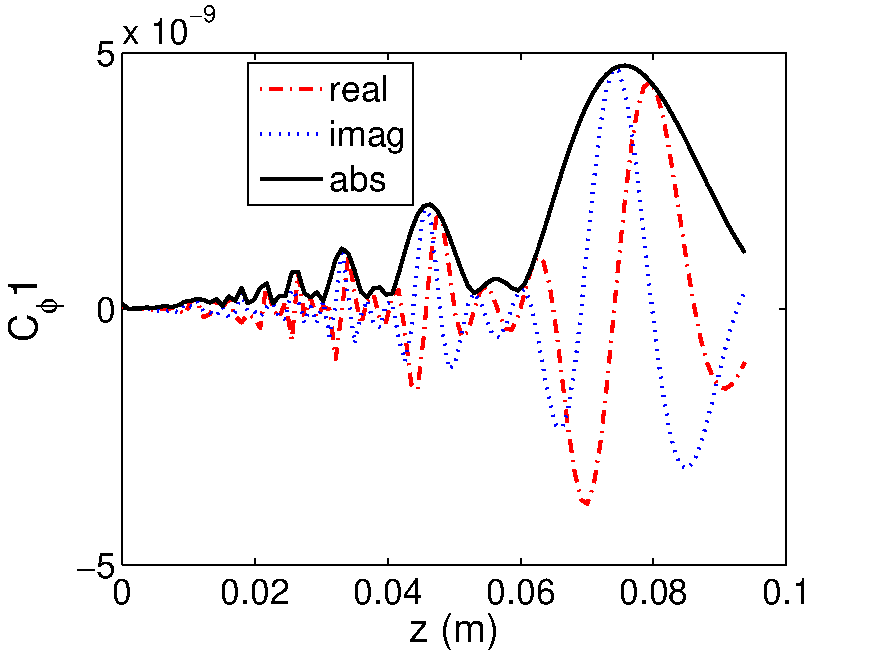
\includegraphics[scale=.44]{../media/Figs/Cphi1}}
\end{minipage}%
\begin{minipage}{.5\linewidth}
\centering
\subfloat[$ \mathcal{C}_\phi(z) $ for $ r_\perp > a $]{\label{Czd}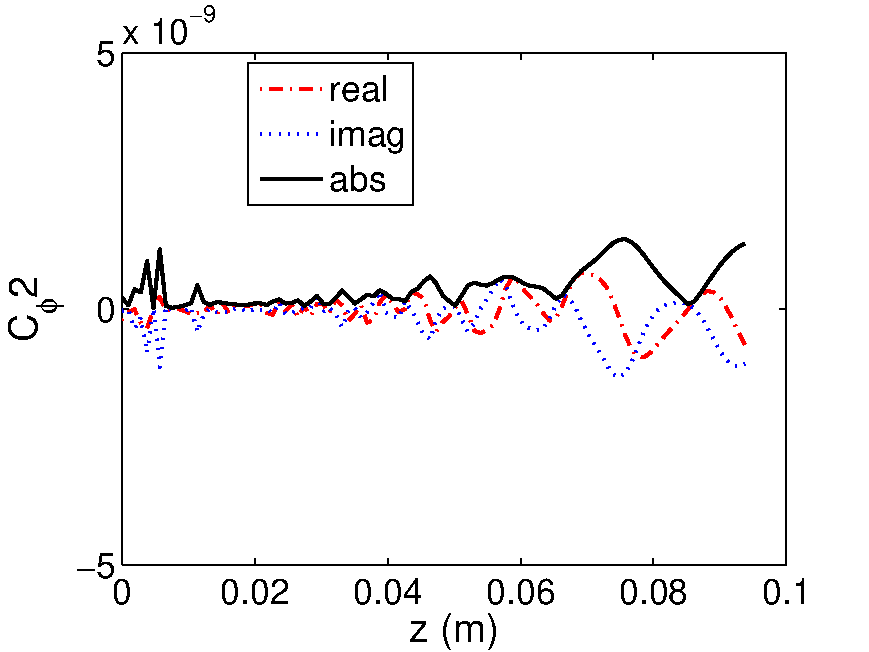
\includegraphics[scale=.44]{../media/Figs/Cphi2}}
\end{minipage}
\caption{$ \mathcal{C}^{(\omega,p=+,f=+)}(z) $. The values of these coefficients are in an arbitrary unit. }
\label{Cz}
\end{figure}




\begin{figure}[H] 
\centering
\subfloat[$ \mathcal{A}(z) $]{\label{Az}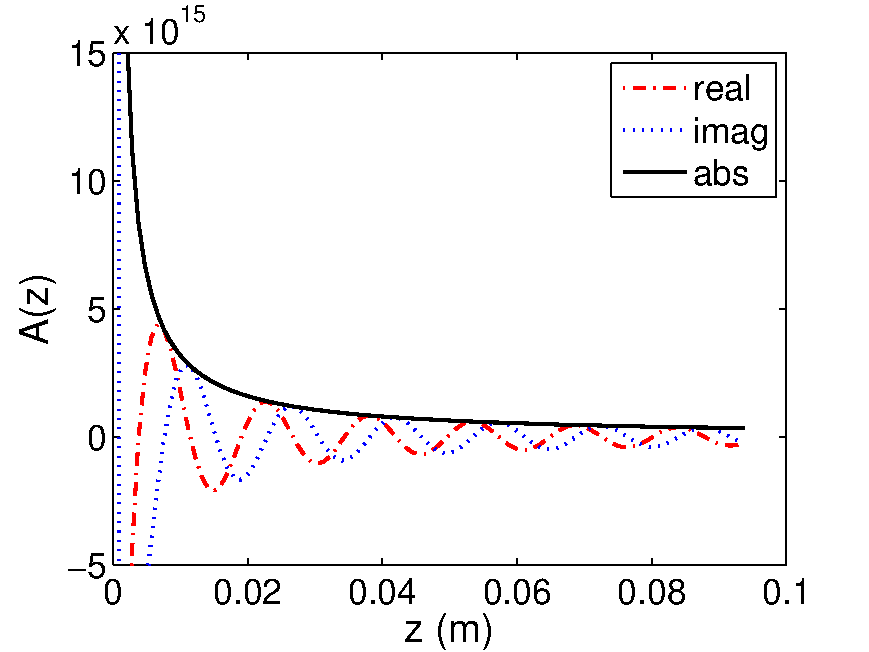
\includegraphics[scale=.5]{../media/Figs/Az}}
\par\medskip
\begin{minipage}{.5\linewidth}
\centering
\subfloat[$ \mathcal{C}_{r_\perp}(z) $]{\label{Crz}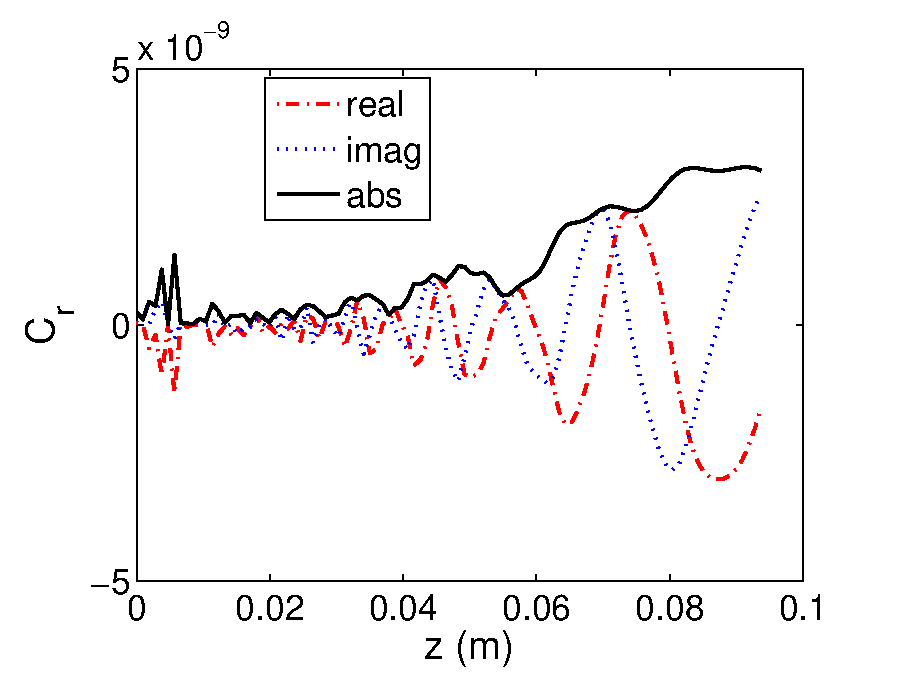
\includegraphics[scale=.44]{../media/Figs/Cr}}
\end{minipage}%
\begin{minipage}{.5\linewidth}
\centering
\subfloat[$ \mathcal{C}_\phi(z) $ ]{\label{Cphiz}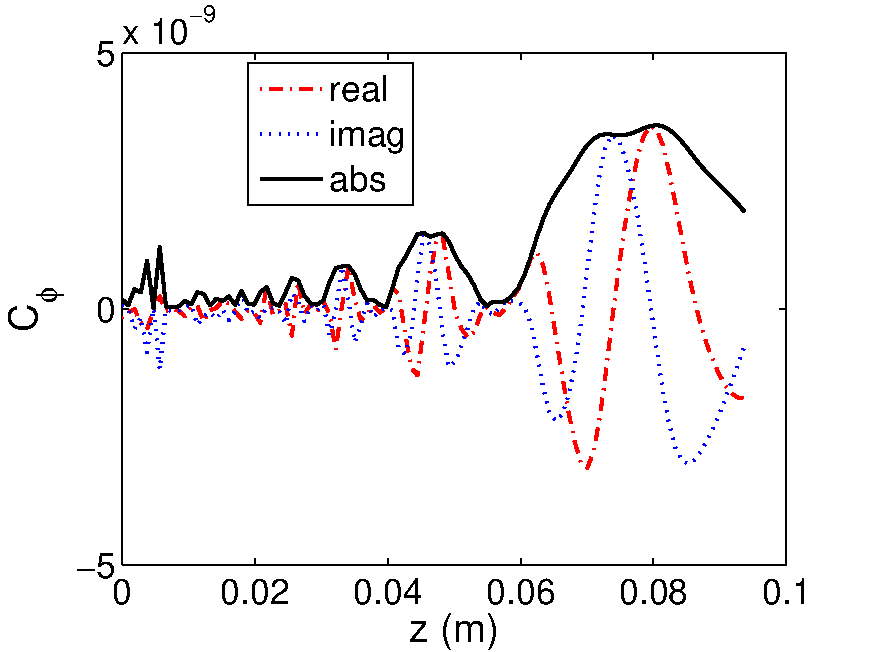
\includegraphics[scale=.44]{../media/Figs/Cphi}}
\end{minipage}
\par\medskip
\begin{minipage}{.5\linewidth}
\centering
\subfloat[$ \mathcal{S}_{r_\perp}(z) $ ]{\label{Srz}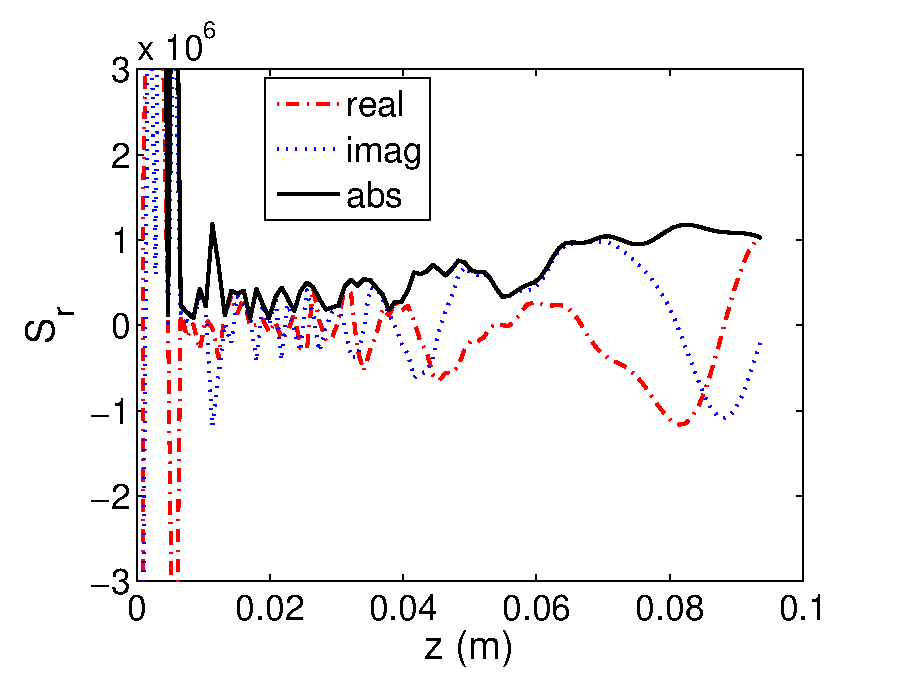
\includegraphics[scale=.44]{../media/Figs/Sr}}
\end{minipage}%
\begin{minipage}{.5\linewidth}
\centering
\subfloat[$ \mathcal{S}_\phi(z) $]{\label{Sphiz}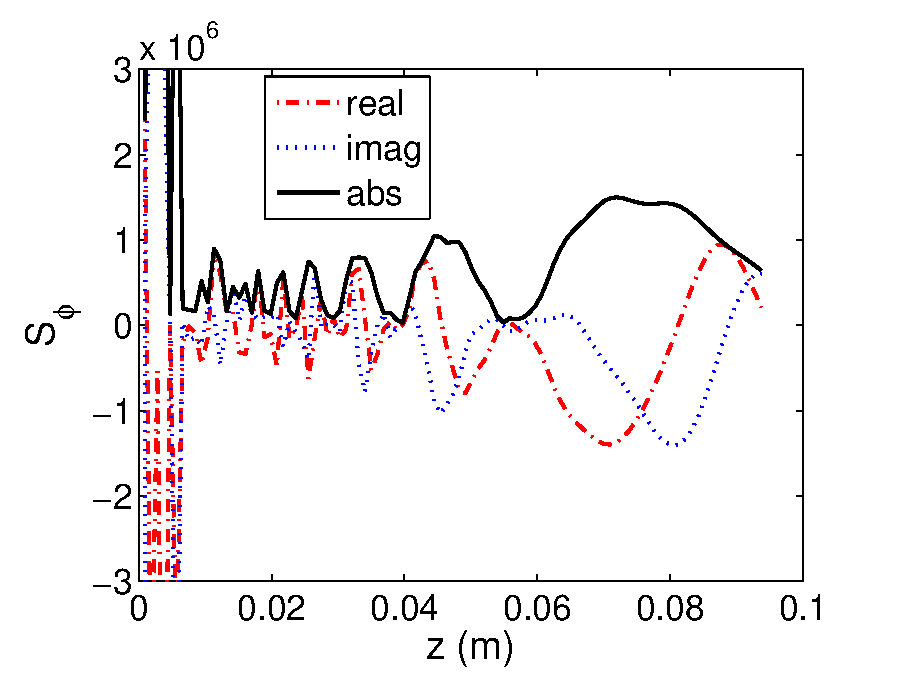
\includegraphics[scale=.44]{../media/Figs/Sphi}}
\end{minipage}
\caption{$ \mathcal{A}(z) $, $ \mathcal{C}^{(\omega,p=+,f=+)}(z) $ and $ \mathcal{S}^{(\omega,p=+,f=+)}(z) $. The values of these coefficients are in an arbitrary unit. There should be some fast chopping in $ \mathcal{A}(z) $ and $ \mathcal{S}^{(\mu)}(z) $. However, due to the cost of computing time, we did not give a fine enough calculation in our plots. See following plots for the calculation results with an improved resolution.  }
\label{ACSz}
\end{figure}


\scalefig{../media/Figs/InterferencePeriods}{0.6}{Wave path-difference of the interference between a monochromatic light emitted from a point atom located at $ \br'=(r'_\perp,\phi',z')=(2a,0,0) $ and a laser beam propagating along the $ z $-axis at the same wavelength $ \lambda_0=937.1 $ nm. The  horizontal axis of the plot is scaled in terms of the radium $ a $ of the nanofiber. The vertical axis is the wave path-difference measured along the laser's propagation direction of $ z $-axis, which is scaled by the wavelength $ \lambda=\lambda_0 $. As we can see, the interference period is uniform, and is on the order of $ 4.2a $.  This rough calculation implies that the chopping frequency in $ z $-direction should on the order of the wavelength, which should be reflected in Fig.~\ref{ACSz} and related plots. }


\newpage
Notice that, calculation resolution matters to the results. For comparison, we run the exact simulation as above but with a better $ z $-resolution.  The results are shown in Figs.~\ref{Cz_1} and~\ref{ACSz_1}. In $ z\in (0,1)\,\mathrm{mm} $ region, we calculate the coefficients in every $ 20 $ wavelengths; in $ z\in[2,100]\,\mathrm{mm} $ region, we calculate the coefficients in every $ \lesssim 1000 $ wavelengths. While in Figs.~\ref{Cz} and~\ref{ACSz} before, we calculate the coefficients evenly in every $ 1000 $ wavelengths. Also, when we calculated the integrals in the figures below, we used a $ 3 $ times better resolution in $ r_\perp\in(a,5a) $ region, which gives more detailed features of the $ \mathcal{C}^{(\mu)} (z)$ and $ \mathcal{S}^{(\mu)}(z) $ plots. With this improved resolution, it takes more than one hour to run the full calculation on a Thinkpad X200 laptop. 

\begin{figure}[H] 
\begin{minipage}{.5\linewidth}
\centering
\subfloat[$ \mathcal{C}_{r_\perp}(z) $ for $ r_\perp < a $]{\label{Cza_1}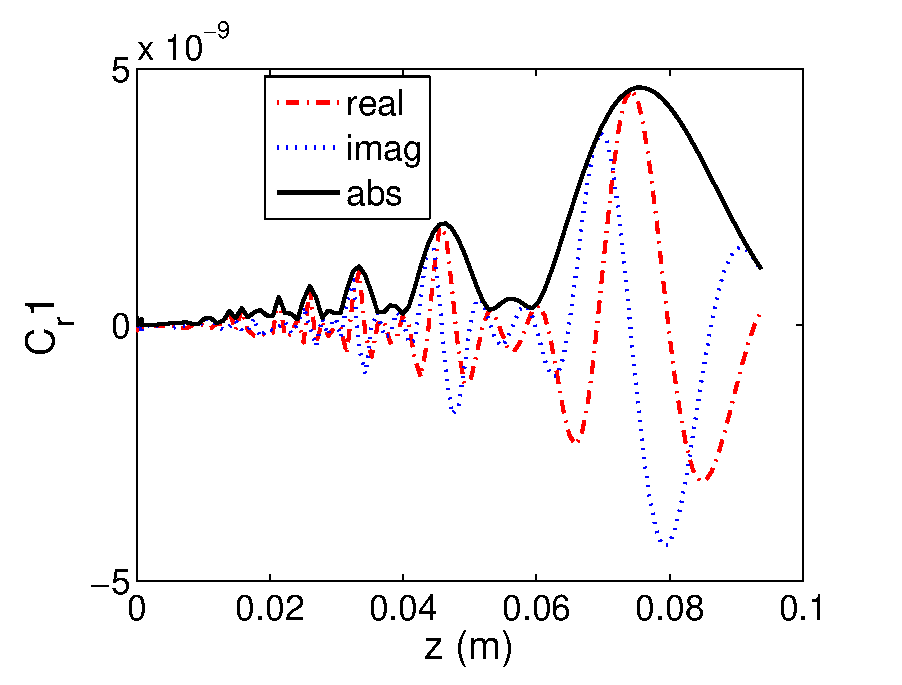
\includegraphics[scale=.44]{../media/Figs/Cr1_1}}
\end{minipage}%
\begin{minipage}{.5\linewidth}
\centering
\subfloat[$ \mathcal{C}_{r_\perp}(z) $ for $ r_\perp > a $]{\label{Czb_1}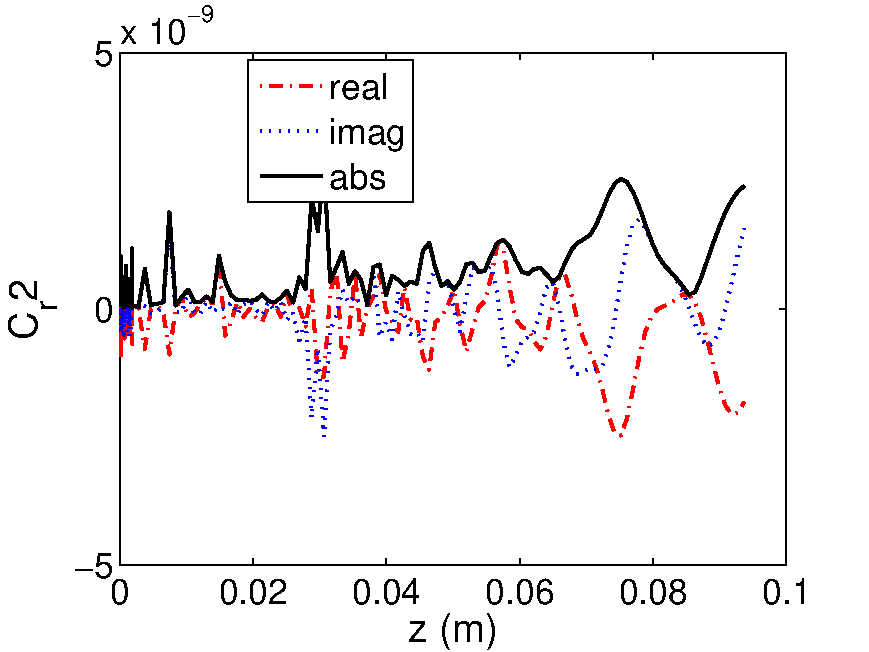
\includegraphics[scale=.44]{../media/Figs/Cr2_1}}
\end{minipage}
\par\medskip
\begin{minipage}{.5\linewidth}
\centering
\subfloat[$ \mathcal{C}_\phi(z) $ for $ r_\perp < a $]{\label{Czc_1}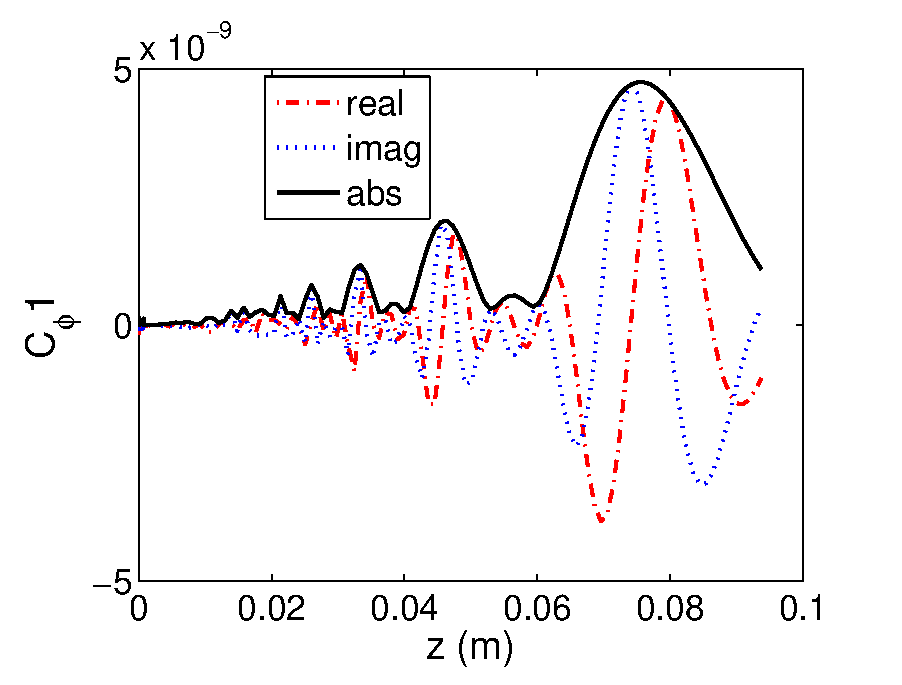
\includegraphics[scale=.44]{../media/Figs/Cphi1_1}}
\end{minipage}%
\begin{minipage}{.5\linewidth}
\centering
\subfloat[$ \mathcal{C}_\phi(z) $ for $ r_\perp > a $]{\label{Czd_1}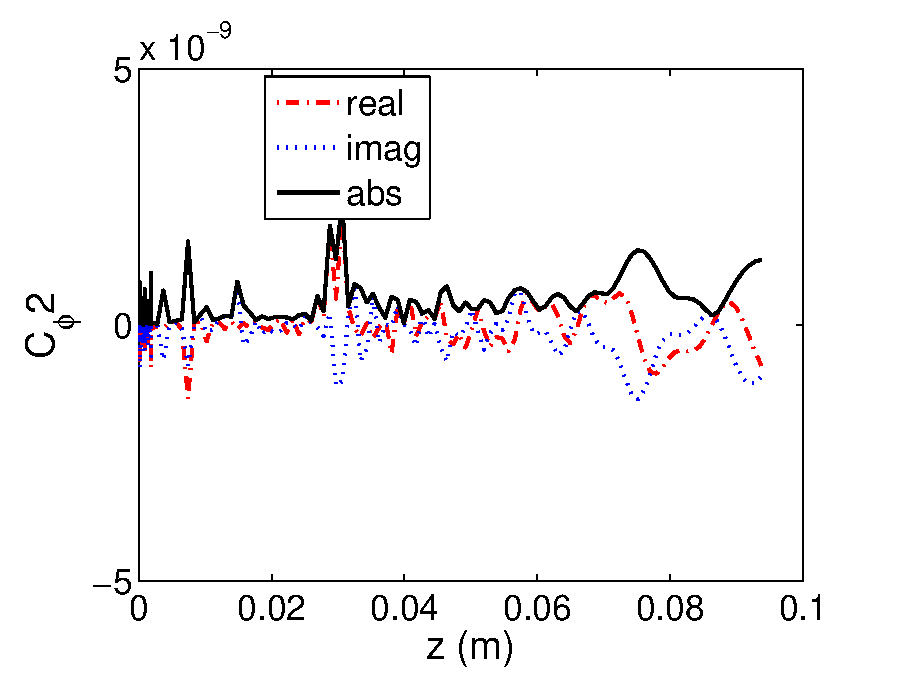
\includegraphics[scale=.44]{../media/Figs/Cphi2_1}}
\end{minipage}
\caption{$ \mathcal{C}^{(\omega,p=+,f=+)}(z) $. The values of these coefficients are in an arbitrary unit. Resolution is improved (see text).}
\label{Cz_1}
\end{figure}




\begin{figure}[H] 
\centering
\subfloat[$ \mathcal{A}(z) $]{\label{Az_1}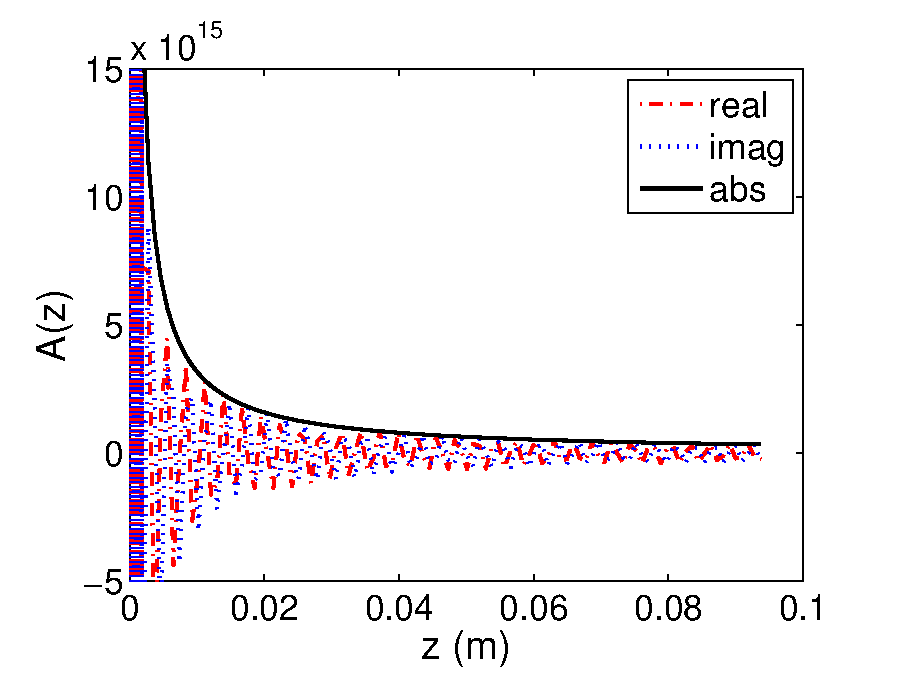
\includegraphics[scale=.5]{../media/Figs/Az_1}}
\par\medskip
\begin{minipage}{.48\linewidth}
\centering
\subfloat[$ \mathcal{C}_{r_\perp}(z) $]{\label{Crz_1}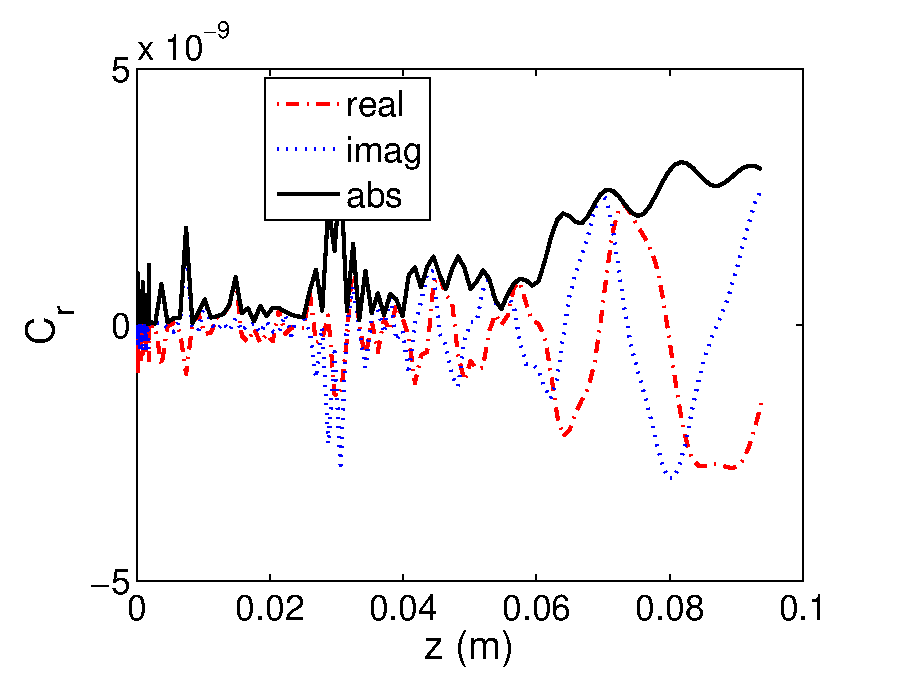
\includegraphics[scale=.42]{../media/Figs/Cr_1}}
\end{minipage}%
\begin{minipage}{.48\linewidth}
\centering
\subfloat[$ \mathcal{C}_\phi(z) $ ]{\label{Cphiz_1}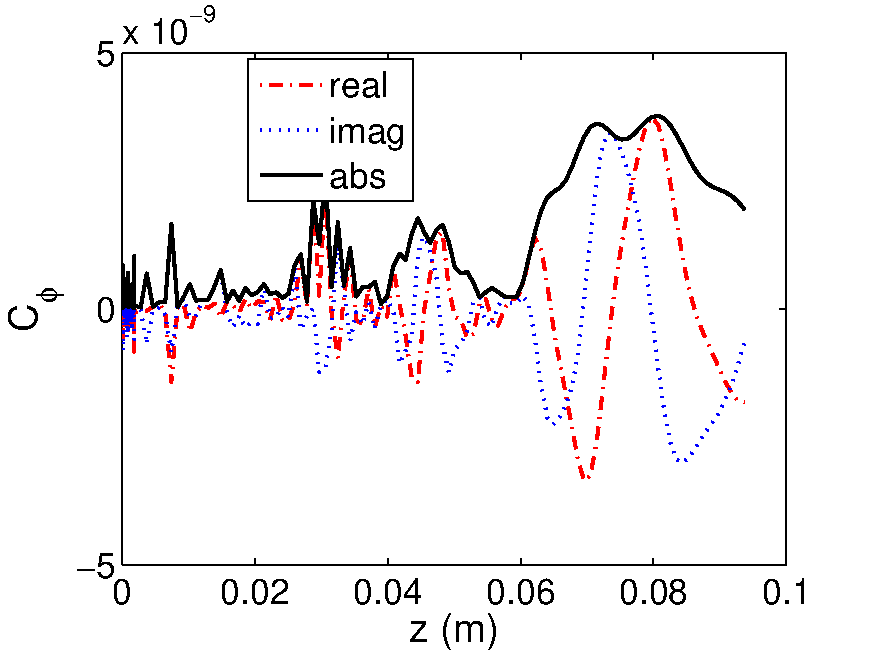
\includegraphics[scale=.42]{../media/Figs/Cphi_1}}
\end{minipage}
\par\medskip
\begin{minipage}{.48\linewidth}
\centering
\subfloat[$ \mathcal{S}_{r_\perp}(z) $ ]{\label{Srz_1}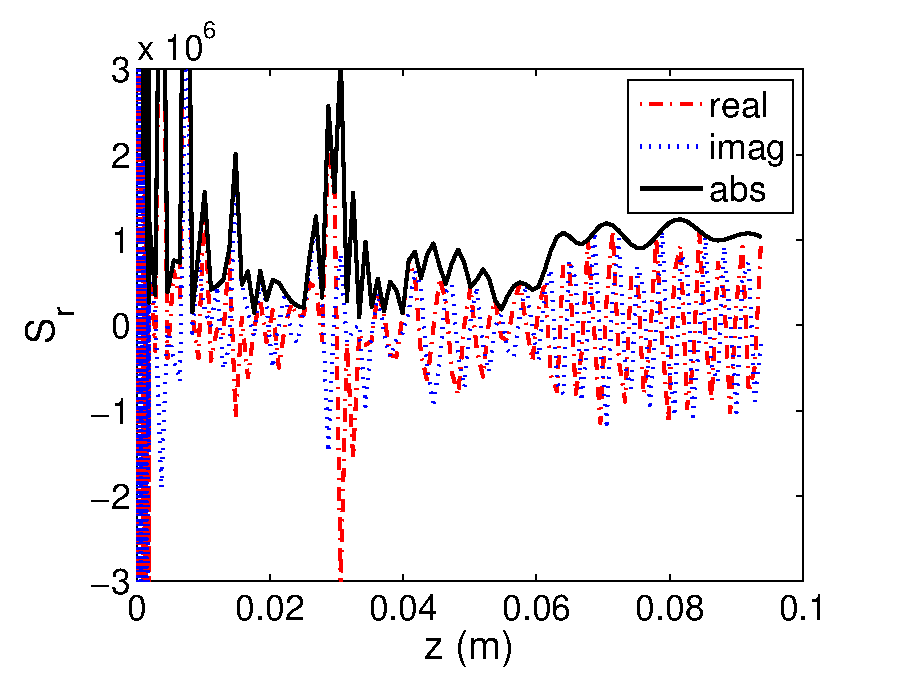
\includegraphics[scale=.42]{../media/Figs/Sr_1}}
\end{minipage}%
\begin{minipage}{.48\linewidth}
\centering
\subfloat[$ \mathcal{S}_\phi(z) $]{\label{Sphiz_1}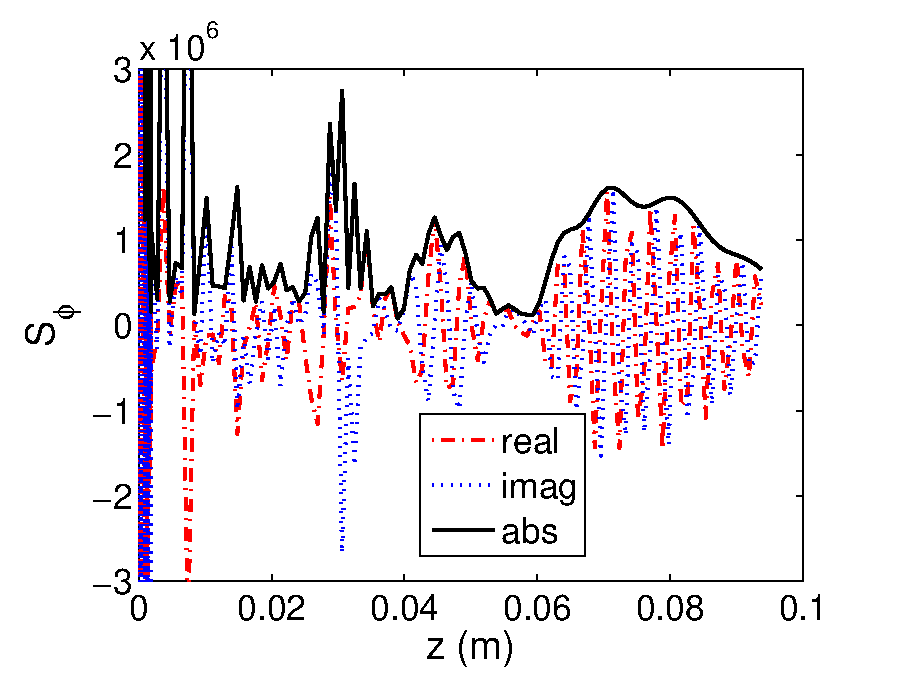
\includegraphics[scale=.42]{../media/Figs/Sphi_1}}
\end{minipage}
\caption{$ \mathcal{A}(z) $, $ \mathcal{C}^{(\omega,p=+,f=+)}(z) $ and $ \mathcal{S}^{(\omega,p=+,f=+)}(z) $. The values of these coefficients are in an arbitrary unit. Resolution is improved (see text).}
\label{ACSz_1}
\end{figure}


\chapter[Finding the magic wavelength for the birefringence protocol]{Finding the magic wavelength for the birefringence QND measurement and spin squeezing protocol for clock-state atoms trapped around a nanofiber}\label{chap:magicwavelength}
In this appendix, we provide some details on finding the magic frequency so that the photon fluctuation noise can be canceled while a QND-measurement-useful Hamiltonian can be retained. We first prove that in the case of one-frequency probe, the scalar polarizability of atoms doesn't allow a magic wavelength for our purpose; then we show that if the scalar polarizability has to be used (for example, to avoid photon scatterings among atoms), a two-color scheme may be feasible; finally, we provide some details on calculating the magic wavelength with one-color probe considering the tensor polarizability effect. We will only take the example of nanofiber, but the theory can be generalized to other nanophotonic waveguides.

Based on Chapter~\ref{chap:birefringence}, in the case that a nanofiber dispersively coupled to an atomic ensemble, the Hamiltonian per time $ \tau $ measurement can be given as below using the Stokes operators, $\hat{S}_q $, and collective spin operators, $ \hat{J}_q $, with $ q=0,1,2,3 $:
\begin{align}
H_{\rm eff} 
=\frac{\hbar}{\tau} \Big\{ & \left[ \big( \chi_{H,\uparrow} + \chi_{H,\downarrow}\big) + \big(\chi_{V,\uparrow} + \chi_{V,\downarrow}\big) \right] \hat{J}_0 \hat{S}_0 \nonumber \\
+ & \left[ \big( \chi_{H, \uparrow} + \chi_{H,\downarrow}\big) - \big( \chi_{V,\uparrow} + \chi_{V,\downarrow} \big)\right]  \hat{J}_0 \hat{S}_1 \nonumber \\
+ & \left[ \big( \chi_{H,\uparrow} - \chi_{H,\downarrow}\big) + \big(\chi_{V,\uparrow} - \chi_{V,\downarrow} \big) \right] \hat{J}_3 \hat{S}_0 \nonumber \\
+ & \left[ \big( \chi_{H,\uparrow} - \chi_{H,\downarrow}\big) - \big(\chi_{V,\uparrow} - \chi_{V,\downarrow} \big) \right]  \hat{J}_3 \hat{S}_1\Big\}.\label{eq:JScoupling}
\end{align}
If we want to estimate the state of the collective 
spins, we need to estimate the number of atoms sitting in the $ \ket{\uparrow} $ and $ \ket{\downarrow} 
$ states employing a dispersive QND measurement technique which has been well developed for the 
free-space atomic ensembles. For our system, the forth term of the Hamiltonian in 
Equ.~\eqref{eq:JScoupling} empowers us the possibility of measuring the atomic states without 
destroying them with an $ \hat{S}_3=\frac{1}{2i}(\hat{a}_H^\dagger\hat{a}_V - 
\hat{a}_V^\dagger\hat{a}_H) $ homodyne measurement. Yet, the third term of the Hamiltonian becomes 
a source of noise term that brings in photon number fluctuation noise into the measurement result. We want to find a magic wavelength of the probe light which allows us to totally remove the third term. For simplicity, we call the third line of the Hamiltonian as $ \hat{H}^3_{\rm eff} $ and its coefficient before the $ \hat{J}_3\hat{S}_0 $ or the corresponding coupling strength as $ \chi_3 $; similarly, we label with the number $ 4 $ for the fourth term of the Hamiltonian and its strength of coupling. We also denote the coupling strength in the fourth term of the Hamiltonian as $ \chi_{\rm eff} $ for the purpose of designing the measurement protocol.


\section{Magic wavelength does not exist with merely scalar polarizability using a simple strategy}
First, we look at the case that the atomic polarizability tensor is reduced to a scalar, which maintain the polarization state of the light in the process of interaction. There are many ways to physically realize such an effect for atoms. 
Here, we assume the detuning of the optical field is much larger than the natural linewidth of the 
coupled atoms so that we can ignore the tensor contribution of the atomic polarizability. We have also 
restricted the atomic ground state within the $ 6S_{1/2} $ $ F=3 $ ($ \ket{\downarrow} $) and $ F=4 $ ($ 
\ket{\uparrow} $) clock state space\index{state!clock state} which rules out the vector contribution of 
the atomic polarizability. Therefore, the atomic polarizability only has a scalar polarizability effect for this problem. 

From the definition of the coupling strength of various $ \chi $'s (Equs.~\eqref{chiHUp} through~\eqref{eq:AeffV}), one can show that, for $ D_1 $ line, 
\begin{align}
\chi_H \equiv \chi_{H,\uparrow} - \chi_{H,\downarrow} &= \frac{1}{3}\sum_{f'} \left(\frac{\sigma_0}{A_{\rm eff}^H} \right) \left(\frac{\Gamma}{4\Delta_{4f'}} - \frac{\Gamma}{4\Delta_{3f'}} \right) \nonumber\\
&= \frac{\Gamma_H}{3} \left(\frac{1}{\Delta_{43}}+\frac{1}{\Delta_{44}} - \frac{1}{\Delta_{33}}-\frac{1}{\Delta_{34}} \right) = \frac{\Gamma_H}{3}\Delta_-,\label{eq:chiH}\\
\chi_V \equiv \chi_{V,\uparrow} - \chi_{V,\downarrow} &= \frac{1}{3}\sum_{f'} \left(\frac{\sigma_0}{A_{\rm eff}^V} \right) \left(\frac{\Gamma}{4\Delta_{4f'}} - \frac{\Gamma}{4\Delta_{3f'}} \right) \nonumber\\
&= \frac{\Gamma_V}{3} \left(\frac{1}{\Delta_{43}}+\frac{1}{\Delta_{44}} - \frac{1}{\Delta_{33}}-\frac{1}{\Delta_{34}} \right)=\frac{\Gamma_V}{3}\Delta_-,\label{eq:chiV}
\end{align}
where $ \Delta_{ff'} $ is the detuning relative to the $ f\leftrightarrow f' $ transition gap, and $ \Delta_- = \left(\frac{1}{\Delta_{43}}+\frac{1}{\Delta_{44}} - \frac{1}{\Delta_{33}}-\frac{1}{\Delta_{34}} \right) $ is a common factor existing in both $ \chi_H $ and $ \chi_V $ quantities. $ \Gamma_H $ ($ \Gamma_V $) is the decay rate coupled to the forward propagating $ H $ ($ V $) mode of the nanofiber. 

To find the \emph{magic wavelength}\index{magic wavelength}, we need to make the coupling strength factor of the third term of the Hamiltonian in Equ.~\eqref{eq:JScoupling} equal to zero. That is to say,
\begin{align}
\chi_H+\chi_V=\frac{1}{3}\left(\Gamma_H + \Gamma_V \right)\Delta_- = 0.
\end{align}
We can see that $ \frac{1}{3}\left(\Gamma_H + \Gamma_V \right) $ is always positive and does not 
depending on wavelength. Therefore, we have to let $ \Delta_-=0 $ to find the "\textit{magic 
wavelength}"\index{magic wavelength}. From the definition of $ \chi_H $ and $ \chi_V $ 
(Equs.~\eqref{eq:chiH} and~\eqref{eq:chiV}) and the Hamiltonian (Equ.~\eqref{eq:JScoupling}), we can 
find that $ \chi_H=\chi_V=0 $ and the forth term of the Hamiltonian, which is what we want to keep, also 
becomes zero. Hence, via identifying a magic wavelength and to remove the photon flux noise in the 
measurement is invalid for our initial design. Maybe we can say, the \emph{magic wavelength}\index{magic wavelength} does not 
exist for one-color probe configuration and by only considering scalar polarizability effects. 

This analytical conclusion has been numerically verified. 

\section{Calculating coupling strengths with a scalar polarizability}
Now, let us suppose we target to generating a spin squeezed state (SSS) based on the forth term of the Hamiltonian through an $ \hat{S}_3 $ homodyne QND measurement. The effective Hamiltonian becomes
\begin{align}
	H_{\rm eff} = \frac{\hbar}{\tau} \chi_{\rm eff} \hat{J}_3 \hat{S}_1
\end{align}
where $\chi_{\rm eff} = \chi_{H} - \chi_{V}=\frac{\Gamma_H-\Gamma_V}{3}\Delta_-$. As has been proved, the squeezing parameter $ \xi =\frac{\chi_{\rm eff}^2 }{4}N_LN_A $. Therefore, to calculate the squeezing parameter, we need to calculate the decay rates coupled into the $ H $ and $ V $ modes. 

Since we can treat the atomic polarizability as a scalar for our dispersive case, we have 
\begin{align}
\Gamma_H &= 2\pi \sum_g \frac{|\mathbf{u}_H(\br')\cdot \mathbf{d}_{eg}|^2}{\hbar}\left(\frac{\omega_0}{v_g} \right) \\
&\propto \sum_g \tr \left\{(\mathbf{d}_{eg}^*\mathbf{d}_{eg})\cdot \mathrm{Im} [\GFT_H^*(\br',\br')] \right\}  = \sum_f \tr \left[ \alpha_f \eye\cdot \mathrm{Im} [\mathbf{G}_H^*(\br',\br')]  \right],
\end{align}
where the atomic polarizability for the ground state $ f $ is defined as $ \alpha_f=\alpha_0(\Delta_{ff'})C_{j'f}^{(0)} $ is a scalar constant for the clock state. Using the emission surface technique introduced in Sec.~\ref{sec:geometryofemission}, the equivalent dipole momentum is pointed along $ [1,1,1]/\sqrt{3} $ direction on the principle emission coordinate system induced by the fiber $ H $-mode field. Since the $ H $ mode only has $ r\!_\perp $ and $ z $ components for an atom on the $ H $ axis, the field only couples to the corresponding $ \mathbf{e}_x $ and $ \mathbf{e}_z $ two dipole orientations with a normalization factor $ 1/3 $ for the $ D_1 $ line transitions. Similar conclusion applies to the $ \Gamma_V $ calculation yet with a $ y $ coupling. One can also consider this problem in the perspective of quantum jumps. Since all quantum transitions ($ \pi$ and $\sigma_\pm $) have the same possibility ($C_{j'ff'}^{(0)}=C_{j'f}^{(0)}=1/3 $), the decay rate is only determined by the non-zero field components with corresponding quantum transition probability. The final result does not depend on how we define the quantization axis while the details of calculation might be. 



With the knowledge of the equivalent dipole orientations, we can easily calculate the corresponding decay rates goes into the forwarding $ H $ and $ V $ modes respectively using the dipole approximation of the atom. Plots below (Figs.~\ref{fig:HVdecayrates} and~\ref{fig:squeezingparaTerms}) illustrate the decay rates and the normalized squeezing parameter $ \xi/N_LN_A $ as functions of frequency and atom positions relative to the fiber axis. $ N_L $ is the photon number counted through the photon detector during time $ \tau $ of measurement. Note that we have assumed that the decay rate is a constant within the small detuning around the D1 line transition frequency, which should be valid. Also, in Fig.~\ref{fig:squeezingparaTerms}, we made up a toy model that we assume both the third and fourth lines of the Hamiltonian alone can generate some spin squeezing with respect to $ \hat{J}_3 $ by some "technical" measurement strategies in time $ \tau $. We plot out the squeezing parameters associated with those two Hamiltonian terms in (a) and (b) of Fig.~\ref{fig:squeezingparaTerms}. If both (a) and (b) have similar values at the same frequency and atom position points, it means the coupling effect to both Hamiltonians overlap and the useful spin squeezing with the realistic Hamiltonian (in presence of both Hamiltonian terms) will be weak. If there are mismatches on the data points, in contrast, it means one can design some protocol to obtain a strong spin squeezing effect. Based on the plots, one can hardly design a good spin squeezing protocol based on the properties of the Hamiltonian. 

\begin{figure}[!tbp]
\begin{minipage}{.91\linewidth}
\centering
{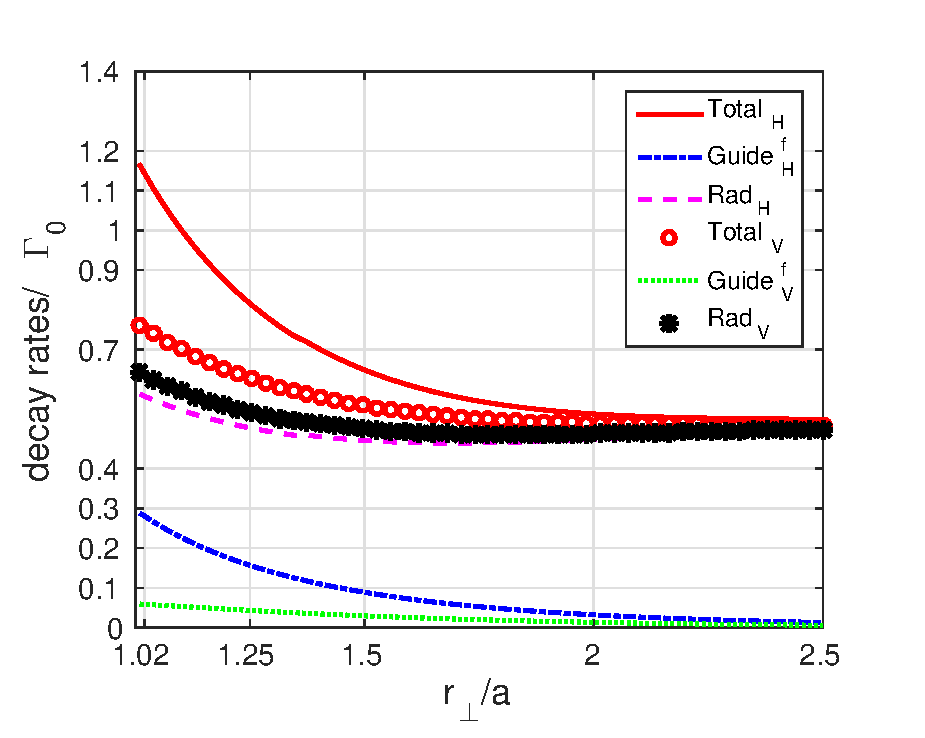
\includegraphics[scale=0.75]{../media/Figs/HVdecayrates}}
\end{minipage}
\caption[Decay rates coupled to the $ H $ and $ V $ nanofiber modes with a scalar polarizability of atoms.]{Decay rates coupled to the $ H $ and $ V $ nanofiber modes. For the guided mode contributions, only the forward propagating mode contributions are plotted out. The total decay rates for the two mode contributions have both backward and forward propagating components counted.}\label{fig:HVdecayrates}
\end{figure}

\begin{figure}[!tbp]
\begin{minipage}{.91\linewidth}
\centering
\subfloat[]{\label{squeezingparaTerm3}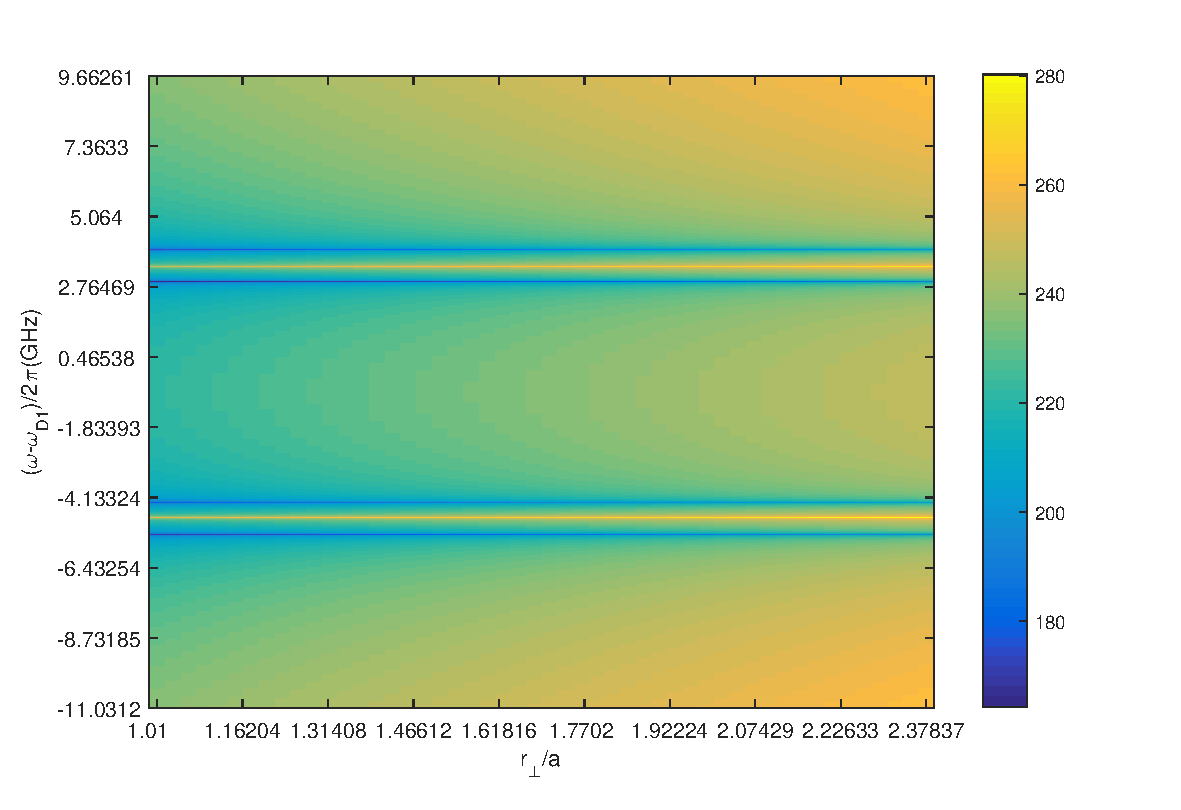
\includegraphics[scale=0.55]{../media/Figs/squeezingparaTerm3}}
\end{minipage}
\par\medskip
\begin{minipage}{.91\linewidth}
\centering
\subfloat[]{\label{squeezingparaTerm4}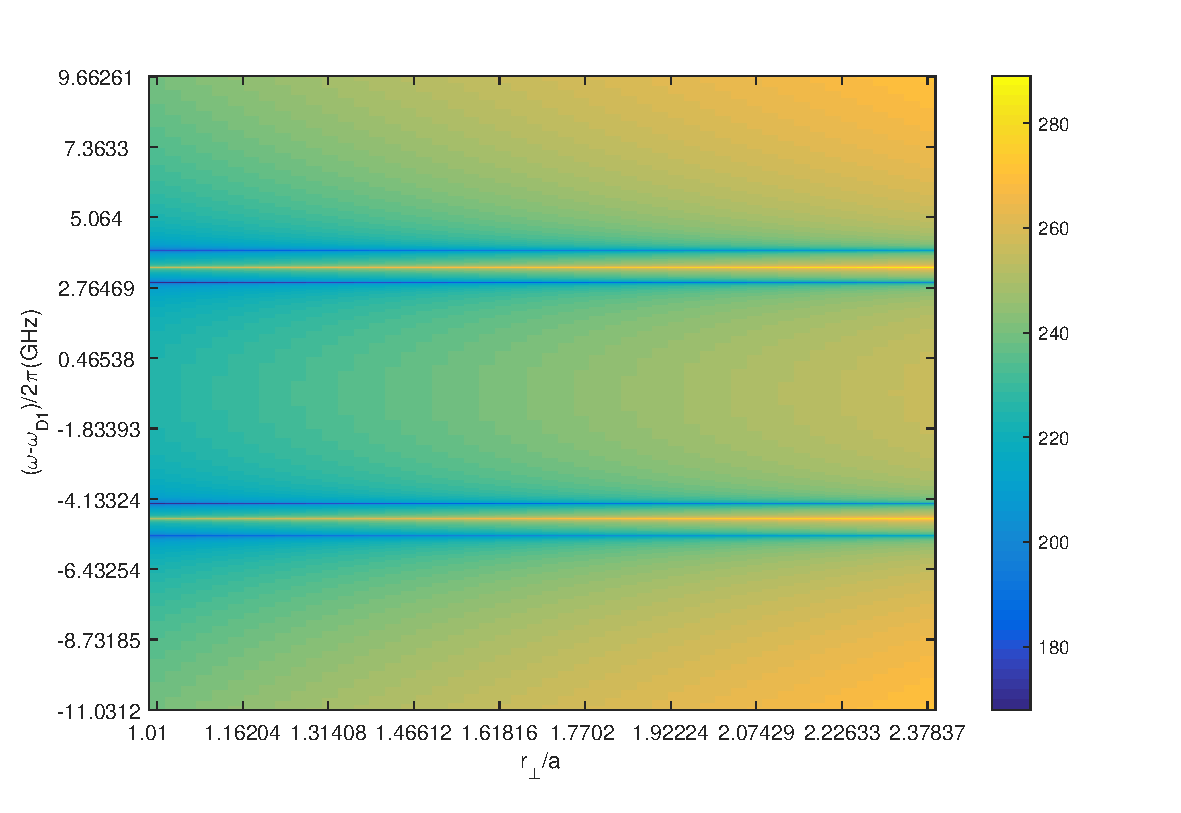
\includegraphics[scale=0.55]{../media/Figs/squeezingparaTerm4}}
\end{minipage}
\caption[Squeezing parameters as a function of frequency and the atoms' radial position using a scalar polarizability in a toy model.]{Squeezing parameters associated with the third (a) and forth (b) terms of the Hamiltonian as a function of frequency and the atoms' radial position (see text). The colormap shows the value of $ -10\log_{10}(\xi/N_LN_A) $, where $ \xi $ is the squeezing parameter and $ N_L $ is the photon number counted at the photon detector in time period $ \tau $. The calculation assumes the signal is solely generated by $ \hat{H}^3_{\rm eff} $ and $ \hat{H}^4_{\rm eff} $, respectively, which is just a toy model. We use this simulation to show the possibility of designing a good spin squeezing protocol by finding a proper frequency and some atom positions. }
\label{fig:squeezingparaTerms}
\end{figure}

\begin{figure}
\begin{minipage}{.91\linewidth}
\centering
{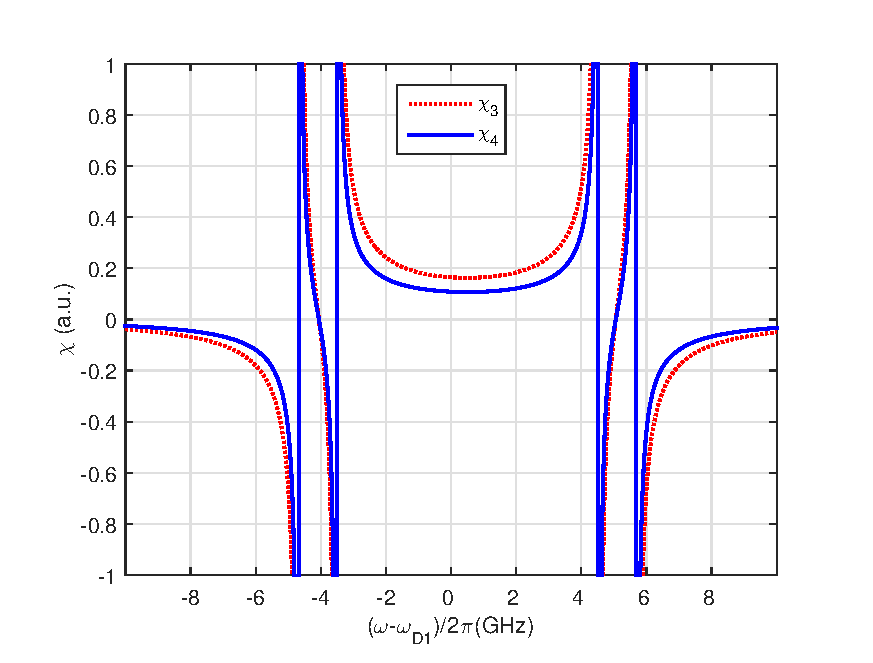
\includegraphics[scale=0.75]{../media/Figs/chi34}}
\end{minipage}
\caption[Coupling strengths as a function of detuning.]{The coupling strengths for the third ($ \chi_3 $) and forth ($ \chi_4 $) terms of the Hamiltonian expressed in Eq.~\eqref{eq:JScoupling} for the D1 line transitions associated with the clock states.} \label{fig:chi34}
\end{figure}

As shown in Fig.~\ref{fig:chi34} regarding the coupling strengths of the third and forth terms of the one-color probe Hamiltonian, the two peaks on the negative frequency side and those on the positive frequency side correspond to the approximate frequencies one can use to detect the $ \ket{\uparrow} $ and $ \ket{\downarrow} $ atom numbers. The two Hamiltonian terms seem very close to each other due to the small $ \Gamma_V $. How much the photon fluctuation affects the final result is unclear, but the noise is on the same order as the signal (projection noise).



\section{Estimate psuedo-spin state and atom number in a high resolution}
Now we come to the question "is there any way to remove the photon fluctuation from the homodyne measurement?" One way that might work is to use two-color light signals to commit the measurement. The basic idea follows. 

If we use two-color probes for each measurement configuration, it might be possible to find non-trivial magic wavelengths to cancel the third term of the Hamiltonian. The key is that, for two distinguishable colors, the decay rates coupled to the corresponding guided modes are distinguishable as well, which may result in magic wavelengths that does not totally remove the coupling strengths at the same time. For instance, if we choose the two probes around D1 and D2 transition frequencies at $ \omega_1 $ and $ \omega_2 $, the two sets of $ \Gamma_{H/V}(\omega_1) $ and $ \Gamma_{H/V}(\omega_2) $ will be different. Quantitatively, the third term of the effective Hamiltonian can now be given by
\begin{align}
\!\!\!\!\!\!\!\!\!\!\hat{H}_{\rm eff}^3(\omega_1,\omega_2) &= \frac{\hbar}{\tau} \left[\chi_H(\omega_1)+\chi_H(\omega_2) + \chi_V(\omega_1)+\chi_V(\omega_2) \right] \hat{J}_3\hat{S}_0\\
&= \frac{\hbar}{3\tau} \left[  \left( \Gamma_H(\omega_1)\!+\!\Gamma_V(\omega_1) \right)\Delta_-^1(\omega_1) \!+\! 2\left( \Gamma_H(\omega_2)\!+\!\Gamma_V(\omega_2) \right)\Delta_-^2(\omega_2) \right] ,
\end{align}
where $ \Delta_-^{1/2} $ are the detuning terms due to the two colors of the probes. Similarly, the forth term of the Hamiltonian can now be given by
\begin{align}
\!\!\!\!\!\!\!\!\!\!\hat{H}_{\rm eff}^4(\omega_1,\omega_2) &= \frac{\hbar}{\tau} \left[\chi_H(\omega_1)+\chi_H(\omega_2) - \chi_V(\omega_1)-\chi_V(\omega_2) \right] \hat{J}_3\hat{S}_0\\
&= \frac{\hbar}{3\tau} \left[  \left( \Gamma_H(\omega_1)\!-\!\Gamma_V(\omega_1) \right)\Delta_-^1(\omega_1) \!+\! 2\left( \Gamma_H(\omega_2)\!-\!\Gamma_V(\omega_2) \right)\Delta_-^2(\omega_2) \right] .
\end{align}
Now that, the magic wavelengths canceling the third term of the Hamiltonian may not result in a zero coupling strength for the forth term of the Hamiltonian due to the inseparability of decay rates and detuning factors. A two-color scheme has been tested in experiments by the QUANTOP group in Denmark for QND measurement~\cite{Beguin2014}, but it's more about using the differential phase shifts between the two probes to magnify the signal-to-noise ratio than using an precise magic wavelength to cancel the noise sources. 


\section{Magic wavelength exists by including tensor polarizability effect}
Finally, if we include the tensor polarizability effect into the Hamiltonian, and use the $ x $-axis as the 
quantization axis, the Hamiltonian can still be given in the form of Eq.~\ref{eq:JScoupling} yet with a 
tensor-response definition of the coupling strengths:
\begin{align}
\chi_{H,\uparrow/\downarrow} & \equiv \chi_{H,f} =- \frac{2\pi \omega_0}{v_g} \bra{f,0} 
	\mathbf{u}^*_H(r^\prime\!_\perp, \phi') \cdot \tensor{\alpha} \cdot 
	\mathbf{u}_{H}(r^\prime\!_\perp, 
	\phi') \ket{f,0} \\
	& =- \frac{2\pi \omega_0}{v_g} \sum_{f'} \sum_q \alpha_0\left( f,f'  \right) |\mathbf{e}_q \cdot 
	\mathbf{u}_H^*(r^\prime\!_\perp,\phi')|^2 |o^{j'f'}_{jf} |^2 
	|C^{f 0;1q}_{f' q}|^2\\
	& \approx  \frac{1}{2} \left( \sigma_0 n_g  \right) \sum_{f'} \sum_q\left( 
		\frac{\Gamma}{2 
		\left(\Delta_{f,f'}+i\Gamma/2\right) }  \right)\nonumber\\
		&\quad\quad\quad\quad\quad\quad\quad\quad\quad \times |\mathbf{e}_q \cdot 
		\mathbf{u}_H^*(r^\prime\!_\perp,\phi')|^2 |o^{j'f'}_{jf} |^2 
		|C^{f 0;1q}_{f' q}|^2,\\
\chi_{V,\uparrow/\downarrow} & \equiv \chi_{V,f} =- \frac{2\pi \omega_0}{v_g} \bra{f,0} 
	\mathbf{u}^*_V(r^\prime\!_\perp, \phi') \cdot \tensor{\alpha} \cdot 
	\mathbf{u}_{V}(r^\prime\!_\perp, 
	\phi') \ket{f,0} \\
	& =- \frac{2\pi \omega_0}{v_g} \sum_{f'} \sum_q \alpha_0\left( f,f'  \right) |\mathbf{e}_q \cdot 
	\mathbf{u}_V^*(r^\prime\!_\perp,\phi')|^2 |o^{j'f'}_{jf} |^2 
	|C^{f 0;1q}_{f' q}|^2\\
	& \approx  \frac{1}{2} \left( \sigma_0 n_g  \right) \sum_{f'} \sum_q\left( 
		\frac{\Gamma}{2 
		\left(\Delta_{f,f'}+i\Gamma/2\right) }  \right)\nonumber\\
		&\quad\quad\quad\quad\quad\quad\quad\quad\quad \times |\mathbf{e}_q \cdot 
		\mathbf{u}_V^*(r^\prime\!_\perp,\phi')|^2 |o^{j'f'}_{jf} |^2 
		|C^{f 0;1q}_{f' q}|^2,
\end{align}
where we have approximated $ \lambda_{j'}\approx \lambda = \frac{2\pi c}{\omega_0} $.  

The magic wavelengths/frequencies using the one-probe configuration can be found close to the $ 
f=3\rightarrow f'=3 $ and $ f=4\rightarrow f'=4 $ two transitions.
The spin squeezing parameters solely due to $ \hat{H}^3_{\rm eff} $ and $ \hat{H}^4_{\rm eff} $ can be calculated for our toy model as has been discussed earlier.
Plots for the coupling strengths and magic frequencies can be found in 
Figs.~\ref{fig:MagicwavelengSqueezingpara},~\ref{fig:squeezingparaTerms_total} 
and~\ref{fig:chi34_total}.

\begin{figure}[!tbp]
\begin{minipage}{.91\linewidth}
\centering
\subfloat[]{\label{MagicwavelengSqueezingpara1}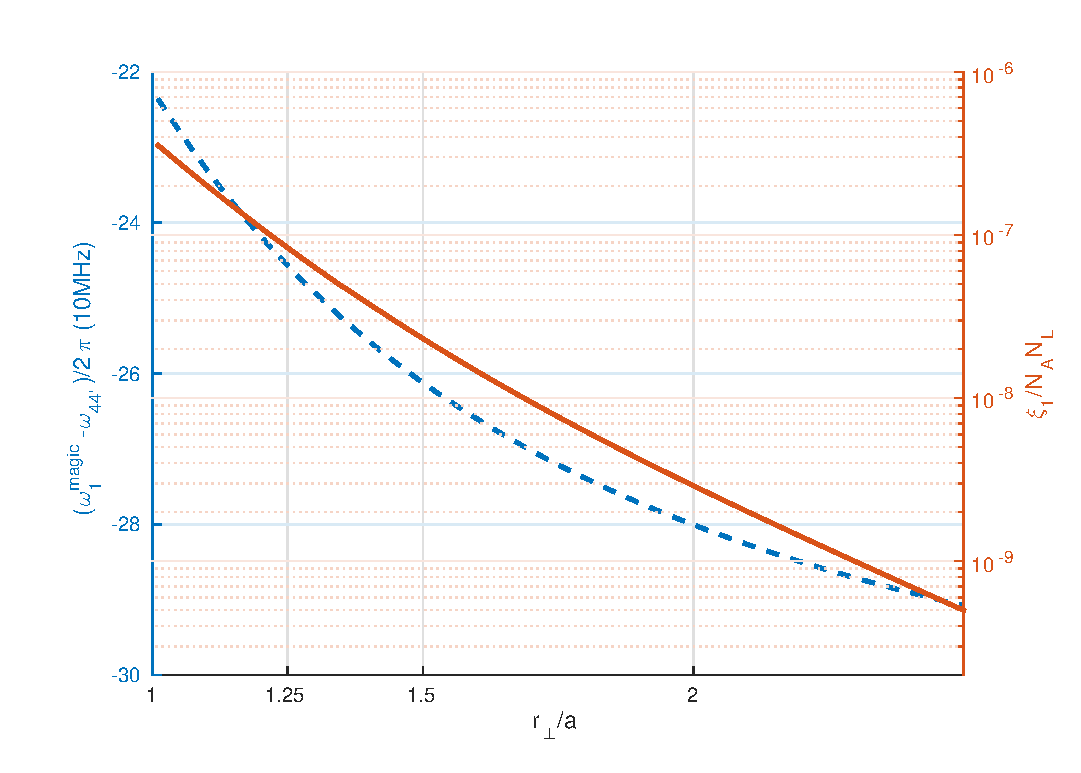
\includegraphics[scale=0.65]{../media/Figs/MagicwavelengSqueezingpara1}}
\end{minipage}
\par\medskip
\begin{minipage}{.91\linewidth}
\centering
\subfloat[]{\label{MagicwavelengSqueezingpara2}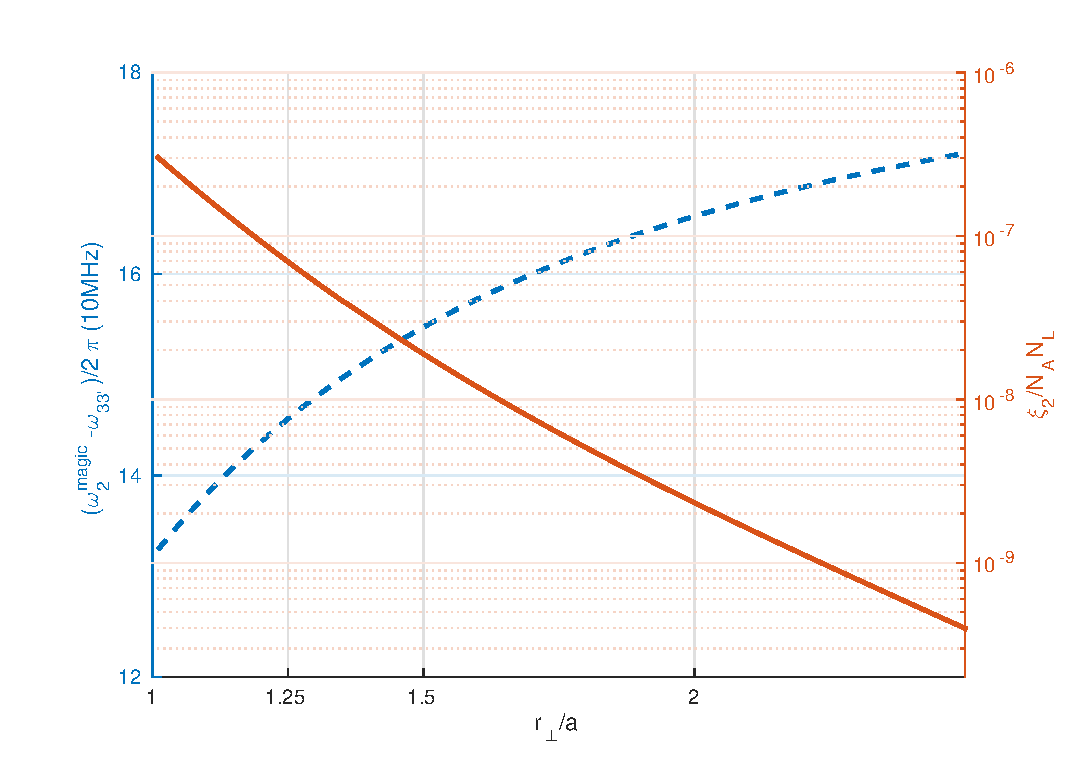
\includegraphics[scale=0.65]{../media/Figs/MagicwavelengSqueezingpara2}}
\end{minipage}
\caption[Magic frequencies and spin squeezing including the tensor interactions.]{The magic frequencies (left axis and dashed lines) and corresponding squeezing parameters 
(right axis and solid lines) close to the $ 
f=3\rightarrow f'=3 $ (b) and $ f=4\rightarrow f'=4 $ (a) transition lines. The squeezing parameters are 
normalized for per photon per atom squeezing. }\label{fig:MagicwavelengSqueezingpara}
\end{figure}

\begin{figure}[!tbp]
\begin{minipage}{.91\linewidth}
\centering
\subfloat[]{\label{squeezingparaTerm3_total}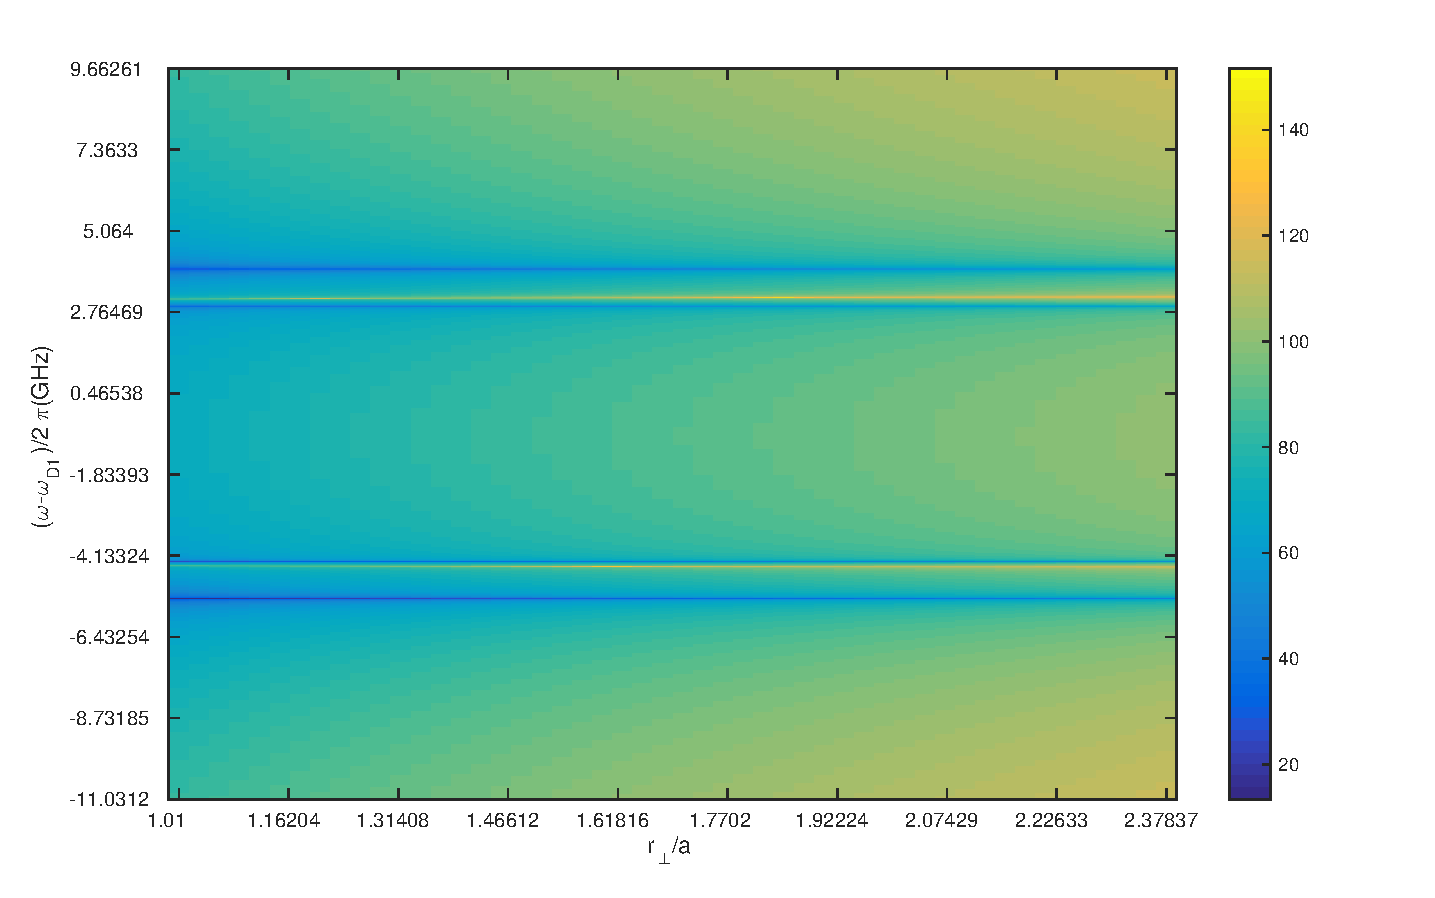
\includegraphics[scale=0.55]{../media/Figs/squeezingparaTerm3_total}}
\end{minipage}
\par\medskip
\begin{minipage}{.91\linewidth}
\centering
\subfloat[]{\label{squeezingparaTerm4_total}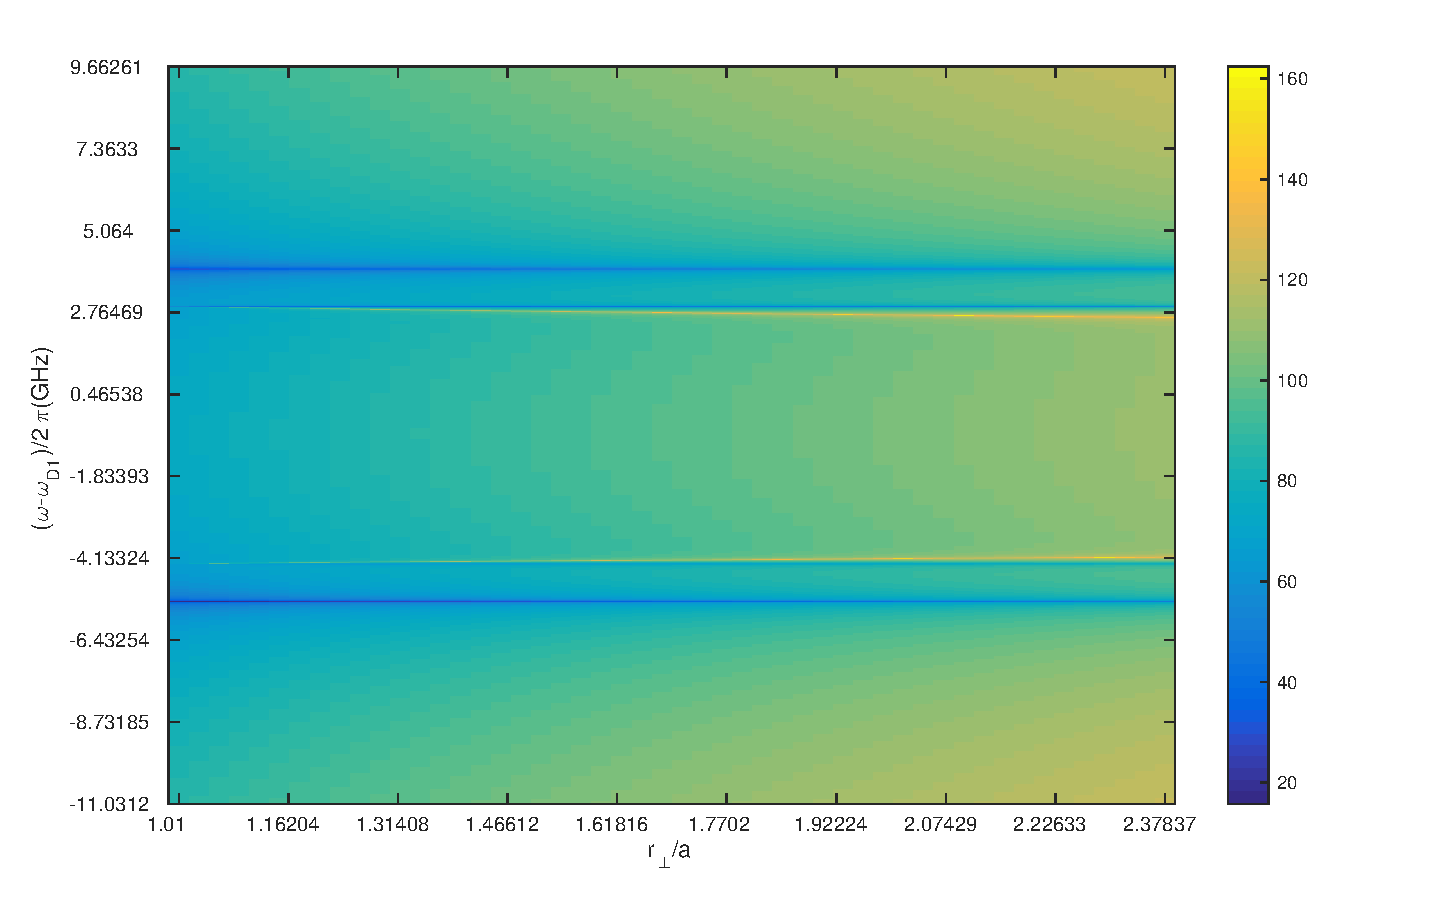
\includegraphics[scale=0.55]{../media/Figs/squeezingparaTerm4_total}}
\end{minipage}
\caption[Squeezing parameters as a function of detuning and atom position with a full atomic polarizability.]{Similar to Fig.~\ref{fig:squeezingparaTerms}, squeezing parameters associated with the third (a) and forth (b) terms of the Hamiltonian in a toy model. The 
colormap shows the value of $ -10\log_{10}(\xi/N_LN_A) $.  All atomic polarizability components are included. We see there are some pattern-mismatch areas to design a good spin squeezing protocol to cancel the noise sources while still retain a strong useful coupling Hamiltonian.}
\label{fig:squeezingparaTerms_total}
\end{figure}

\begin{figure}[!tbp]
\begin{minipage}{.91\linewidth}
\centering
{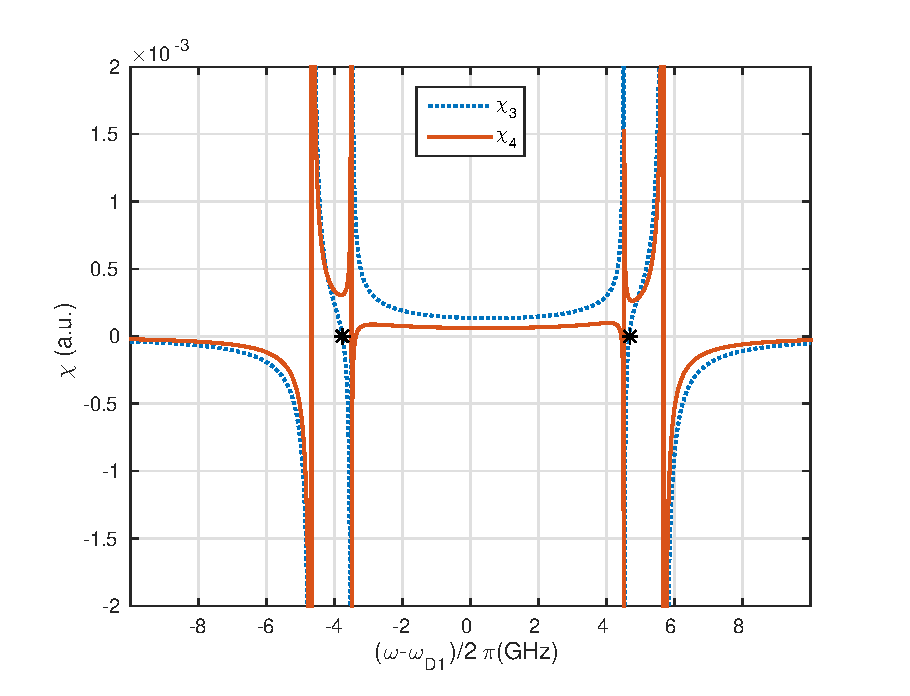
\includegraphics[scale=0.75]{../media/Figs/chi34_total}}
\end{minipage}
\caption[The coupling strengths in the birefringence-interaction Hamiltonian 
calculated for the D1 line transitions associated with the clock states to find the magic frequencies.]{The coupling strengths, $ \chi_3 $ and $ \chi_4 $, in the Hamiltonian 
expressed in Eq.~\eqref{eq:JScoupling} calculated for the D1 line transitions associated with the clock states.
All atomic polarizability components are included. The stars indicate where the magic frequencies are existed. The value of $ \chi_4 $ is considerable at the two magic frequencies.}  
\label{fig:chi34_total}
\end{figure}


%\bibliographystyle{amsplain}
\bibliographystyle{unsrt}
% \nocite{*}
\ifwindows
	\bibliography{F:/References/Archive/Archive}
\else
	\bibliography{/media/F/References/Archive/Archive}
\fi

\printindex

\end{document}          
